% **********************************************************
% sicp
%
% Structure and Interpretation of Computer Programs, 2e
% Unofficial Texinfo Format
%
% This file is licensed under a Creative Commons
% Attribution-ShareAlike 4.0 International License
% (http://creativecommons.org/licenses/by-sa/4.0/).
%
% For more information about this file, see the text under
% "\label{UTF}" below.
%
% Various versions of sicp.texi and preformatted sicp.info
% can be found at the following Web pages:
%
%   http://www.neilvandyke.org/sicp-texi/
%   http://sicpebook.wordpress.com/
%
% **********************************************************

% HISTORY:
%
% * Version 1 (April, 2001) by Lytha Ayth.
%
% * Version 2 (April 20, 2001) by Lytha Ayth.
%
% * Version 2.nwv1 (March 11, 2002) by Neil W. Van Dyke.
%   Cosmetic change to heading in Info format, and comment changes.
%
% * Version 2.neilvandyke1 (February 10, 2003) by Neil W. Van Dyke
%   Correction to Exercise 1.39 formula, spotted by Steve VanDevender.
%   Added URL of Abelson and Sussman video lectures.
%
% * Version 2.neilvandyke2 (unreleased)
%
% * Version 2.neilvandyke3 (April 20, 2006) by Neil W. Van Dyke
%   Pedro Kr\"oger patch to add missing Lisp example.
%
% * Version 2.neilvandyke4 (January 10, 2007) by Neil W. Van Dyke
%   Brad Walker patch to add \code{@dircategory} and \code{@direntry}.
%
% * Version 2.andresraba1 (May 23, 2011) by Andres Raba.
%   Mathematics typeset in TeX, figures redrawn in vector graphics,
%   typeface changed, cross-references improved, hyperlinks added,
%   known errors and typos corrected.
%
% * Version 2.andresraba2 (November 21, 2011) by Andres Raba.
%   Minor change to the appearance of diagrams. Adjusted page layout.
%   Fixed some typos. License changed from CC BY-NC to CC BY-SA.
%
% * Version 2.andresraba3 (November 22, 2012) by Andres Raba.
%   Improved layout and pagination. Included list of figures.
%   Added punctuation to displayed math. Updated citation links.
%
% * (Version 2.andresraba4 is the pocket version, described in
%   sicp-pocket.texi.)
%
% * Version 2.andresraba5 (September 20, 2013) by Andres Raba.
%   Texinfo source is converted to LaTeX. Pages are redesigned.
%
% * (Versions 2.andresraba5.{1..3} with minor fixes and additions.)
%
% * Version 2.andresraba5.4 (February 3, 2015) by Andres Raba.
%   Added noncommercial clause to the license. Fixed broken links
%   and added more fulltext links to References. Brian Wignall
%   decapitalized function names at the beginning of sentences.
%
% * Version 2.andresraba5.5 (September 15, 2015) by Andres Raba.
%   Updated license to CC BY-SA 4.0. Redesigned title page.
%   Tinted chapter and section numbers. Fixed broken links.
%
% * Version 2.andresraba5.6 (February 2, 2016) by Andres Raba.
%   Improved microtypography in code listings. Removed manual
%   word breaks. Fixed broken links.

\newcommand{\latestVersion}%
  {community.202606.2}
\newcommand{\latestVersionLink}%
  {https://github.com/junnunkarim/book__sicp_source__latex}

%%%%%%%%%%%%%%%%%%%%%%%%%%%%%%%%%%%%%%%%%%%%%%%%%%%%%%%%%%%%%%%%%%%%%%%%%%%%%%%

\providecommand{\bookClass}{book}

% paperType modes
% ---------------
% 0 -> a5
% 1 -> a4
% 2 -> ustrade
\providecommand{\paperType}{0}

%%%%%%%%%%%%%%%%%%%%%%%%%%%%%%%%%%%%%%%%%%%%%%%%%%%%%%%%%%%%%%%%%%%%%%%%%%%%%%%

% buildChapter modes
% ------------------
% 0 -> all chapters
% 1 -> chapter 1
% 2 -> chapter 2
% 3 -> chapter 3
% 4 -> chapter 4
% 5 -> chapter 5
\providecommand{\buildChapter}{0}

\ifcase\buildChapter % 0
  \newcommand{\buildExtraContents}{1} % true
  \newcommand{\showChapterInfo}{0} % false
\or % 1
  \newcommand{\buildExtraContents}{1} % true
  \newcommand{\showChapterInfo}{1} % true
\else %
  \newcommand{\buildExtraContents}{0} % false
  \newcommand{\showChapterInfo}{1} % true
\fi
 
\providecommand{\buildUnofficialContents}{0} % default is false

\ifcase\paperType % 0 -> a5
  % documentclass
\PassOptionsToClass{%
  a5paper,
  11pt,
}{\bookClass}

\PassOptionsToPackage{
  a5paper,
  headheight=13pt,
  inner=14mm,
  outer=16mm,
  top=20mm,
  bottom=16mm,
}{geometry}

\or % 1 -> a4
  % documentclass
\PassOptionsToClass{%
  a4paper,
  12pt,
}{\bookClass}

\PassOptionsToPackage{
  a4paper,
  headheight=15pt,
  inner=25mm,
  outer=20mm,
  top=25mm,
  bottom=20mm,
}{geometry}

\or % 2 -> ustrade
  % documentclass
\PassOptionsToClass{%
  11pt,
}{\bookClass}

\PassOptionsToPackage{
  paperwidth=6in,
  paperheight=9in,
  headheight=15pt,
  inner=22.225mm,
  outer=19.05mm,
  top=19.05mm,
  bottom=19.05mm,
}{geometry}

\else % default
  % documentclass
\PassOptionsToClass{%
  a5paper,
  11pt,
}{\bookClass}

\PassOptionsToPackage{
  a5paper,
  headheight=13pt,
  inner=14mm,
  outer=16mm,
  top=20mm,
  bottom=16mm,
}{geometry}

\fi


\documentclass[twoside]{\bookClass}

% set font to new computer modern
\usepackage{newcomputermodern}

% configure page margins and dimensions
\usepackage{geometry}

% provide multi-language support
\usepackage{polyglossia}

% enable breakable hyphens within code blocks
\usepackage[shortcuts]{extdash}

% manage image inclusion and manipulation
\usepackage{graphicx}

% provide extensive color support
\usepackage[dvipsnames, x11names]{xcolor}

% provide advanced mathematical typesetting
\usepackage{amsmath}

% offer extended verbatim environments
\usepackage{fancyvrb}

% enable concurrent index generation
\usepackage{imakeidx}

% configure index layout and formatting
\usepackage{idxlayout}

% customize page headers and footers
\usepackage{fancyhdr}

% insert pages from external pdf files
\usepackage[final]{pdfpages}

% change appearance of section titles
\usepackage{titlesec}

% add syntax highlighted code listings
\usepackage{listings}

% provide simple verbatim and comment environments
\usepackage{verbatim}

% customize list and enumeration environments
\usepackage[shortlabels]{enumitem}

% generate drop capitals
\usepackage{lettrine}

% customize table of contents and lists
\usepackage{tocloft}

% adjust paragraph spacing and indentation
\usepackage[indent]{parskip}

% enable multi-column page layouts
\usepackage{multicol}

% prevent awkward page breaks
\usepackage{needspace}

% customize figure and table captions
\usepackage{caption}

% manage counter formatting and dependencies
\usepackage{chngcntr}

% make cross references and urls clickable
\usepackage{hyperref}

% --- colors ---
% --------------
%
\definecolor{DeepGray}{HTML}{464646}
\definecolor{MediumGray}{HTML}{686868}
\definecolor{LightGray}{HTML}{8B8B8B}

\definecolor{LinkRed}{HTML}{80171F}

% code colors
\definecolor{SchemeLight}{HTML}{686868}
\definecolor{SchemeSteel}{HTML}{888888}
\definecolor{SchemeDark}{HTML}{262626}
\definecolor{SchemeBlue}{HTML}{4172A3}
\definecolor{SchemeGreen}{HTML}{487818}
\definecolor{SchemeBrown}{HTML}{A07040}
\definecolor{SchemeRed}{HTML}{AD4D3A}
\definecolor{SchemeViolet}{HTML}{7040A0}
%
% --------------

% used in index
\def\customDotFill{%
  \leavevmode
  \nobreak
  \cleaders \hbox to .44em{\hss.\hss}\hskip 1em plus1fill
  \nobreak
\kern 0pt}

% e.g. MIT etc.
\newcommand{\acronym}[1]{#1}
\newcommand{\uppersc}[1]{{\fontspec[Letters=UppercaseSmallCaps]{Libertinus
Serif}#1}}
\newcommand{\newterm}[1]{\index{#1}\emph{#1}}
\newcommand{\var}[1]{\textsl{#1}}
\newcommand{\code}[1]{\texttt{#1}}
\newcommand{\link}[1]{\hyperref[#1]{#1}}
\newcommand{\heading}[1]{{\sffamily\bfseries #1}}
\newcommand{\dark}{\color{SchemeDark}}

\newcommand{\mono}[1]{%
  \ifmmode%
    \text{\ttfamily\scriptsize #1}%
  \else%
    {\ttfamily\scriptsize #1}%
  \fi%
}
\newcommand{\monoit}[1]{%
  \ifmmode%
    \text{\ttfamily\itshape\scriptsize #1}%
  \else%
    {\ttfamily\itshape\scriptsize #1}%
  \fi%
}

\newenvironment{example}
  {\verbatim\small}
  {\endverbatim}

\newenvironment{smallexample}
  {\verbatim\footnotesize}
  {\endverbatim}

% package: listings
\lstnewenvironment{scheme}[1][]{%
  \lstset{%
    basicstyle=\ttfamily\small\color{SchemeLight},%
    #1%
  }%
}{}

\lstnewenvironment{smallscheme}[1][]{%
  \lstset{%
    basicstyle=\ttfamily\footnotesize\color{SchemeLight},
    #1%
  }%
}{}

\newenvironment{exercises}{%
  \small%
  \Needspace{6\baselineskip}%
  \vspace{2ex}%
  \begin{flushright}%
    \hfill%
    \textbf{\textsf{EXERCISES}}%
    \vspace{-1ex}%
    \newline%
    \rule{0.5\textwidth}{0.2pt}%
  \end{flushright}%
  % no page break after first horizontal rule
  \vspace{1ex}%
  % every paragraph should not have indent
  \setlength{\parindent}{0pt}%
}{%
  % no page break before last horizontal rule
  % \par\nobreak%
  % \noindent%
  % \makebox[\textwidth][c]{\rule{0.5\textwidth}{0.2pt}}%
  \newpage%
}

% --- figure ---
% --------------
%
\NewDocumentEnvironment{imageFigure}{m}{
  \begin{figure}[htbp]%
    \begin{center}%
}{
    \end{center}%
    \caption{#1}%
    \phantomsection%
    \label{Figure \thefigure}%
  \end{figure}
}

\NewDocumentEnvironment{codeFigure}{m}{
  \begin{flushleft}
    \vspace{2ex}
    \needspace{3\baselineskip}
    \captionof{figure}{\( \downarrow \) #1}%
    \phantomsection%
    \label{Figure \thefigure}
    \nopagebreak
}{
  \end{flushleft}
}

\NewDocumentCommand{\fancyQuoteMark}{O{0,0} m}{%
  \begin{picture}(0,0)(0,0)
    \put(#1){\makebox(0,0){\scalebox{3}{\textcolor{LightGray}{#2}}}}
  \end{picture}%
}
%
% --------------

% --- quotes ---
% --------------
%
% #1 -> author name, #2 -> work name, #3 -> extra
\NewDocumentEnvironment{fancyQuote}{O{} O{} O{}}{%
  \def\fqAuthor{#1}%
  \def\fqWork{#2}%
  \def\fqExtra{#3}%

  \vspace{1ex}
  \noindent
  \begin{list}{}{%
    \setlength{\leftmargin}{0.1\textwidth}%
    \setlength{\rightmargin}{0.1\textwidth}%
  }%
  \item[]%
  \fancyQuoteMark[-15,-5]{``}%
  \color{DeepGray}%
  % \sffamily%
  \footnotesize%
  \begingroup%
    \itshape%
}{%
  \endgroup\par
  \makebox[0pt][l]{%
    \hspace{0.8\textwidth}%
    \fancyQuoteMark[15,15]{''}%
  }%
  \ifx\fqAuthor%
    \empty%
  \else%
    \hfill\rule{0.65\linewidth}{0.2pt}\par
    \hfill
    \begin{minipage}[t]{0.65\linewidth}%
      \scriptsize 
      --- \textsc{\fqAuthor}%
      \tiny 
      % check if fqWork is empty or not
      \ifx\fqWork%
        \empty%
      \else%
        \newline\emph{\fqWork}%
      \fi%
      % check if fqExtra is empty or not
      \ifx\fqExtra%
        \empty%
      \else%
        ,\ (\fqExtra)%
      \fi%
    \end{minipage}%
  \fi
  \par
  \vspace{1ex}
  \end{list}
}

% #1 -> quoted content
% #2 -> author name
% #3 -> work name
% #4 -> extra
\newcommand{\chapterQuote}[4]{
  \vspace{-15pt}%
  \vspace{-1ex}%
  \begin{fancyQuote}[#2][#3][#4]%
    #1%
  \end{fancyQuote}%
  \vspace{-1ex}%
  \vspace{20pt}%
}

% 1st quote
% ---------
% #1 -> quoted content
% #2 -> author name
% #3 -> work name
% #4 -> extra
%
% 2nd quote
% ---------
% #5 -> quoted content
% #6 -> author name
% #7 -> work name
% #8 -> extra
\NewDocumentCommand{\chapterDoubleQuote}{m m m m m m m m}{
  \vspace{-15pt}%
  \vspace{-1ex}%
  \begin{fancyQuote}[#2][#3][#4]
    #1%
  \end{fancyQuote}%

  \begin{fancyQuote}[#6][#7][#8]
    #5%
  \end{fancyQuote}%
  \vspace{-1ex}%
  \vspace{20pt}%
}

% #1 -> quoted content
% #2 -> author name
% #3 -> work name
% #4 -> extra
\newcommand{\elegantQuote}[4]{
  \begin{fancyQuote}[#2][#3][#4]%
    #1%
  \end{fancyQuote}%
}
%
% --------------

% measure header font height using sample string
\newlength{\headerHeight}
\settoheight{\headerHeight}{ABCgjpqy}


\geometry{
  a5paper,
  %
  headheight=3\headerHeight,
  inner=14mm,
  outer=16mm,
  top=16mm,
  bottom=18mm,
  % left=19mm,
  % right=19mm,
  %
  % hcentering,
  % showframe,
}

\let\currentChapter\leftmark
\let\currentSection\rightmark
% if currentSection is empty, use currentChapter
\makeatletter
\newcommand{\currentSectionOrChapter}{%
  % expand "rightmark" and store expanded result in "x"
  \begingroup\protected@edef\x{\rightmark}%
  \ifx\x\@empty
  \endgroup\leftmark
  \else
  \endgroup\rightmark
  \fi
}
\makeatother

\newcommand{\headerStyle}{\itshape\small}

\newcommand{\headerPage}{\headerStyle\thepage}
\newcommand{\headerChapterName}{\headerStyle\currentChapter}
\newcommand{\headerSectionName}{\headerStyle\currentSectionOrChapter}

\pagestyle{fancy}

\fancyhf{} % clear all header/footer styles

\renewcommand{\headrulewidth}{0.0pt}
\renewcommand{\chaptermark}[1]{%
  \markboth{\ifnum\value{chapter}>0 \chaptername\ \thechapter.\ \fi #1}{}%
}
\renewcommand{\sectionmark}[1]{%
  \markright{\ifnum\value{section}>0 \thesection.\ \fi #1}{}%
}

% even pages
\fancyhead[LE]{\headerPage}
\fancyhead[RE]{\headerChapterName}
% odd pages
\fancyhead[RO]{\headerStyle \thepage}
\fancyhead[LO]{\headerSectionName}

% for chapter pages
\fancypagestyle{plain}{
  \fancyhf{} % clear all header and footer fields
  \renewcommand{\headrulewidth}{0pt} % remove header line
  \renewcommand{\footrulewidth}{0pt}  % remove footer line
}

% no header/footer in empty pages
\makeatletter
\renewcommand*{\cleardoublepage}{%
  \clearpage
  \if@twoside
    \ifodd\c@page
    \else
      \hbox{}
      \thispagestyle{empty}
      \newpage
      \if@twocolumn
        \hbox{}
        \newpage
      \fi
    \fi
  \fi
}
\makeatother


% multi-language
\setdefaultlanguage[variant=american]{english}
\setotherlanguages{greek}

% from package: hyperref
% customize link colors
\hypersetup{
  pdfauthor={Harold Abelson, Gerald Jay Sussman, Julie Sussman},
  pdftitle={Structure and Interpretation of Computer Programs, 2nd ed.},
  pdfsubject={computer science, programming, abstraction},
  colorlinks=true,
  linkcolor=LinkRed,
  urlcolor=LinkRed,
}

% lettrine - oversized initial letter
% package: lettrine
\renewcommand{\LettrineFontHook}{\color{MediumGray}}
\LettrineRealHeighttrue
% indentation of paragraphs around lettrine
\setlength{\DefaultFindent}{1pt}
\setlength{\DefaultNindent}{0em}

% vertical spacing between paragraphs
\setlength{\parskip}{0.2\baselineskip plus 0.1ex minus 0.1ex}
% \setlength{\parindent}{2em}

% make space after all punctuation identical to the space between words in the
% middle of a sentence.
\frenchspacing

% depth level up to which section headings are automatically numbered.
\setcounter{secnumdepth}{3} % 3 -> upto subsubsection
% depth level up to which toc content is displayed
\setcounter{tocdepth}{3} % 3 -> upto subsubsection

% --- title formats ---
% ---------------------
%
% package: titlesec
%
% label - chapter number
% title - chapter title
%
% \titleformat{⟨command⟩}
%   [⟨shape⟩]
%   {⟨format⟩} % format applied to the whole title (label and text)
%   {⟨label⟩}
%   {⟨sep⟩} % vertical separation between label and title body (when shape is "display")
%   {⟨before-code⟩} % before title body
%   [⟨after-code⟩]
%
% chapters with numbers
\newcommand{\chapterNumberFont}{%
  \fontsize{8em}{0em}%
  \selectfont%
}

\titleformat{\chapter}
  [display]
  {\filleft\sffamily\bfseries}
  {%
    \color{DeepGray}%
    \mdseries%
    \chapterNumberFont%
    \oldstylenums{\thechapter}%
  }
  {1ex} 
  {\color{DeepGray}\large\MakeUppercase}
  [\color{DeepGray}\titlerule]

% chapters without numbers
\titleformat{name=\chapter, numberless}
  [display]
  {\filright\sffamily\bfseries}
  {}
  {1ex}
  {\color{DeepGray}\large\MakeUppercase}
  [\color{DeepGray}\titlerule]

\titleformat{\section}
  {\filright\large\sffamily\bfseries}
  {\color{MediumGray}\thesection}
  {1ex}
  {\MakeUppercase}

\titleformat{\subsection}
  {\filright\large\sffamily\bfseries}
  {\color{MediumGray}\thesubsection}
  {1ex}
  {}

\titleformat{\subsubsection}
  {\filright\normalsize\sffamily\bfseries}
  {\color{LightGray}\thesubsubsection}
  {1ex}
  {}
%
% ---------------------

% --- table of contents ---
% -------------------------
%
\renewcommand{\cfttoctitlefont}{%
  \sffamily\Huge\bfseries%
}

% toc, section indentation
\setlength{\cftsecindent}{0em}
% toc, sub-section indentation
\setlength{\cftsubsecindent}{1em}
% toc, sub-sub-section indentation
\setlength{\cftsubsubsecindent}{2em}

% toc, gap before chapter title
\setlength{\cftbeforechapskip}{0.5ex}
% toc, gap before section title
\setlength{\cftbeforesecskip}{1ex}

% toc, section font style
\renewcommand{\cftsecfont}{\small}
% toc, sub-section font style
\renewcommand{\cftsubsecfont}{\small}
% toc, sub-sub-section font style
\renewcommand{\cftsubsubsecfont}{\small}
%
% -------------------------

% --- figure ---
% --------------
%
% figure counting: <chapter_count>.<figure_count>
% e.g. 1.1, 2.12 etc.
\counterwithin{figure}{chapter}
% label format -> Figure 1.1, Figure 2.12 etc.
\labelformat{figure}{Figure~#1}

% "list of figures", title style
\renewcommand{\cftloftitlefont}{\sffamily\Large\bfseries}
% "list of figures", gap before title
\setlength{\cftbeforeloftitleskip}{-2\baselineskip} 

% caption style
\captionsetup{
  font=footnotesize,
  labelfont=bf,
  labelformat=simple,
  labelsep=newline,
  justification=raggedright,
  singlelinecheck=false
}

\NewDocumentEnvironment{imageFigure}{m}{
  \begin{figure}[htbp]%
    \begin{center}%
}{
    \end{center}%
    \caption{#1}%
    \phantomsection%
    \label{Figure \thefigure}%
  \end{figure}
}

\NewDocumentEnvironment{codeFigure}{m}{
  \begin{flushleft}
    \vspace{2ex}
    \needspace{3\baselineskip}
    \captionof{figure}{\( \downarrow \) #1}%
    \phantomsection%
    \label{Figure \thefigure}
    \nopagebreak
}{
  \end{flushleft}
}

% scheme syntax highlight
% package: listings
\lstset{
  columns=fixed,
  extendedchars=true,
  breaklines=true,
  breakatwhitespace=false,
  breakautoindent=true,
  numbers=left,
  numberstyle=\tiny,
  upquote=true,
  showstringspaces=false,
  sensitive=false,
  mathescape=true,
  escapechar=~,
  alsodigit={>,<,/,-,=,!,?,*},
  alsoletter=',
  morestring=[b]",
  morecomment=[l];,
  %
  % Keyword list taken form functional.py in Pygments package:
  morekeywords={%
    lambda, define, if, else, cond, and, or, case,%
    let, let*, letrec, begin, do, delay, set!, =>, quote,%
    quasiquote, unquote, unquote-splicing, define-syntax, let-syntax,%
    letrec-syntax, syntax-rules%
  },
  % If keywords are quoted, they must not be highlighted:
  emph={%
    'lambda, 'define, 'if, 'else, 'cond, 'and, 'or, 'case,%
    'let, 'let*, 'letrec, 'begin, 'do, 'delay, 'set!, '=>, 'quote,%
    'quasiquote, 'unquote, 'unquote-splicing, 'define-syntax, 'let-syntax,%
    'letrec-syntax, 'syntax-rules%
  },
  emphstyle=\color{SchemeDark},
  % Paint error red:
  emph={[2]error},emphstyle=[2]\color{SchemeRed},%
  % Builtins taken from functional.py:
  emph={%
    [3]*, +, -, /, <, <=, =, >, >=, abs, acos, angle,
    append, apply, asin, assoc, assq, assv, atan,
    boolean?, caaaar, caaadr, caaar, caadar, caaddr, caadr,
    caar, cadaar, cadadr, cadar, caddar, cadddr, caddr,
    cadr, call-with-current-continuation, call-with-input-file,
    call-with-output-file, call-with-values, call/cc, car,
    cdaaar, cdaadr, cdaar, cdadar, cdaddr, cdadr, cdar,
    cddaar, cddadr, cddar, cdddar, cddddr, cdddr, cddr,
    cdr, ceiling, char->integer, char-alphabetic?, char-ci<=?,
    char-ci<?, char-ci=?, char-ci>=?, char-ci>?, char-downcase,
    char-lower-case?, char-numeric?, char-ready?, char-upcase,
    char-upper-case?, char-whitespace?, char<=?, char<?, char=?,
    char>=?, char>?, char?, close-input-port, close-output-port,
    complex?, cons, cos, current-input-port, current-output-port,
    denominator, display, dynamic-wind, eof-object?, eq?,
    equal?, eqv?, eval, even?, exact->inexact, exact?, exp,
    expt, floor, for-each, force, gcd, imag-part,
    inexact->exact, inexact?, input-port?, integer->char,
    integer?, interaction-environment, lcm, length, list,
    list->string, list->vector, list-ref, list-tail, list?,
    load, log, magnitude, make-polar, make-rectangular,
    make-string, make-vector, map, max, member, memq, memv,
    min, modulo, negative?, newline, not, null-environment,
    null?, number->string, number?, numerator, odd?,
    open-input-file, open-output-file, output-port?, pair?,
    peek-char, port?, positive?, procedure?, quotient,
    rational?, rationalize, read, read-char, real-part, real?,
    remainder, reverse, round, scheme-report-environment,
    set-car!, set-cdr!, sin, sqrt, string, string->list,
    string->number, string->symbol, string-append, string-ci<=?,
    string-ci<?, string-ci=?, string-ci>=?, string-ci>?,
    string-copy, string-fill!, string-length, string-ref,
    string-set!, string<=?, string<?, string=?, string>=?,
    string>?, string?, substring, symbol->string, symbol?,
    tan, transcript-off, transcript-on, truncate, values,
    vector, vector->list, vector-fill!, vector-length,
    vector-ref, vector-set!, vector?, with-input-from-file,
    with-output-to-file, write, write-char, zero?%
  },
  emphstyle=[3]\color{SchemeViolet},
  %
  basicstyle=\color{SchemeLight}\ttfamily,
  keywordstyle=\color{SchemeBlue}\bfseries,
  identifierstyle=\color{SchemeDark},
  stringstyle=\color{SchemeGreen},
  commentstyle=\color{SchemeLight}\itshape,
}


% index style
\idxlayout{%
  totoc, % add to toc
  font=footnotesize,
  justific=raggedright,
}

% generate index
\makeindex[options={-s preamble/indexstyle.ist}]


\begin{document}

\VerbatimFootnotes

\frontmatter
\begin{titlepage}
\newgeometry{margin=20mm}
\vspace*{\fill}
\begin{center}
  
  \textbf{%
    {\huge%
      Structure and Interpretation\\
      \textit{of} Computer Programs%
    }%
  }%
  
  \vspace{4mm}
  
  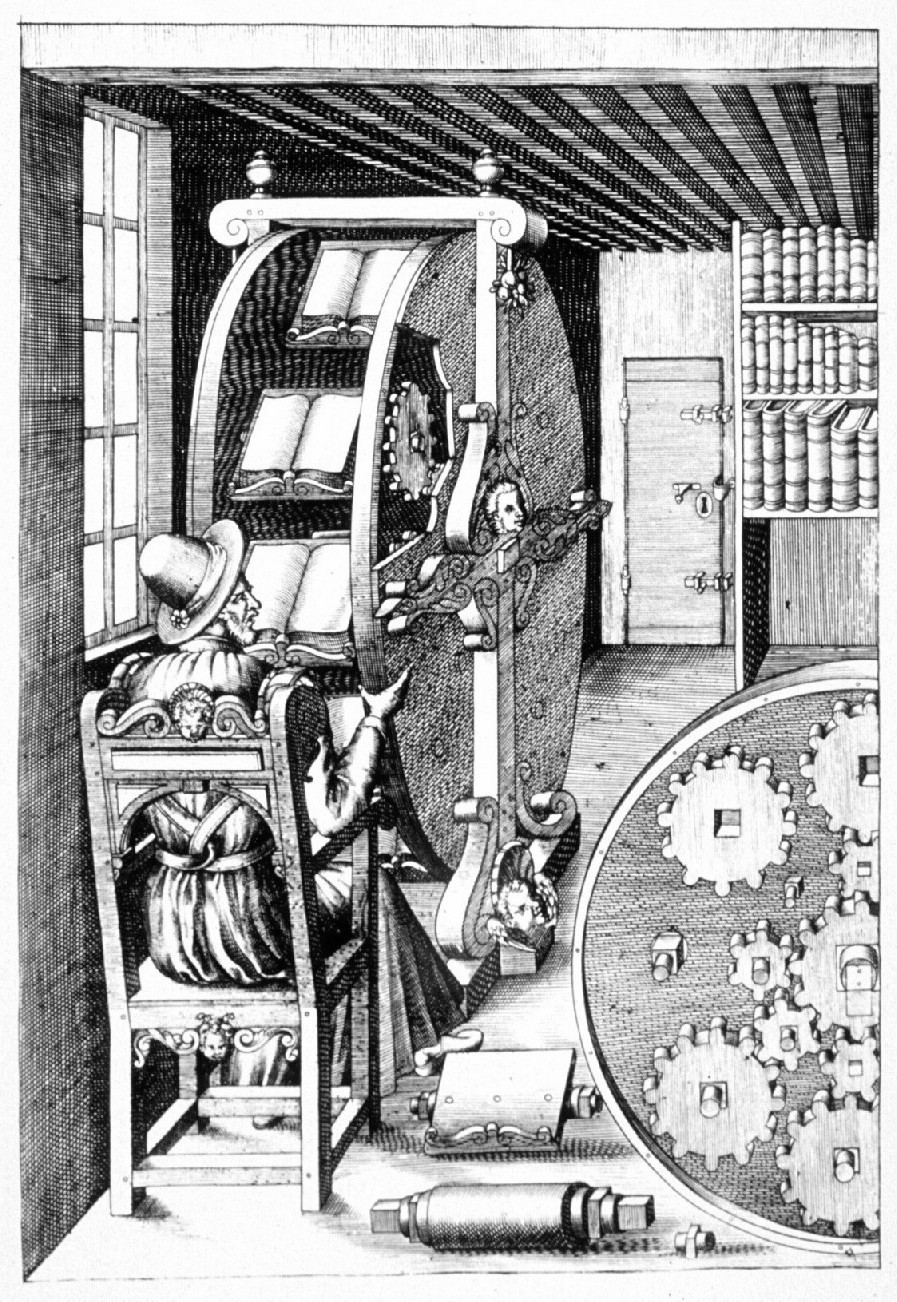
\includegraphics[width=0.45\textwidth]{assets/bookwheel.jpg}

  \vspace{2mm}
  
  {\Large\sffamily\textcolor{LinkRed}{second edition}}\\
  {\small\sffamily version 202606 (community)\par}

  \vspace{1em}

  \Large
  Harold Abelson and\\
  Gerald Jay Sussman\\
  with Julie Sussman\\
  \vspace{0.5em}
  \large
  foreword by Alan J. Perlis
  
\end{center}
\vspace*{\fill}
\restoregeometry
\end{titlepage}

\input{frontmatter/copyright}

\tableofcontents

\label{Top}

\chapter*{Unofficial Texinfo Format}
\markboth{Unofficial Texinfo Format}{}
\addcontentsline{toc}{chapter}{Unofficial Texinfo Format}
\label{UTF}

This is the second edition \acronym{SICP} book, from Unofficial Texinfo
Format.

You are probably reading it in an Info hypertext browser, such as the Info
mode of Emacs.  You might alternatively be reading it {\TeX}-formatted on your
screen or printer, though that would be silly.  And, if printed, expensive.

The freely-distributed official \acronym{HTML}-and-\acronym{GIF} format was
first converted personally to Unofficial Texinfo Format (\acronym{UTF})
version 1 by Lytha Ayth during a long Emacs lovefest weekend in April, 2001.

The \acronym{UTF} is easier to search than the \acronym{HTML} format.  It is
also much more accessible to people running on modest computers, such as
donated '386-based PCs.  A 386 can, in theory, run Linux, Emacs, and a Scheme
interpreter simultaneously, but most 386s probably can't also run both Netscape
and the necessary X Window System without prematurely introducing budding young
underfunded hackers to the concept of \newterm{thrashing}.  \acronym{UTF} can also fit
uncompressed on a 1.44\acronym{MB} floppy diskette, which may come in handy for
installing \acronym{UTF} on PCs that do not have Internet or \acronym{LAN} access.

The Texinfo conversion has been a straight transliteration, to the extent
possible.  Like the {\TeX}-to-\acronym{HTML} conversion, this was not without
some introduction of breakage.  In the case of Unofficial Texinfo Format,
figures have suffered an amateurish resurrection of the lost art of
\acronym{ASCII}.  Also, it's quite possible that some errors of ambiguity
were introduced during the conversion of some of the copious superscripts (`\^{}')
and subscripts (`\_').  Divining \emph{which} has been left as an exercise to
the reader. But at least we don't put our brave astronauts at risk by encoding
the \emph{greater-than-or-equal} symbol as \code{<u>\&gt;</u>}.

If you modify \texttt{sicp.texi} to correct errors or improve the
\acronym{ASCII} art, then update the \code{@set utfversion 2.andresraba5.6}
line to reflect your delta.  For example, if you started with Lytha's version
\code{1}, and your name is Bob, then you could name your successive versions
\code{1.bob1}, \code{1.bob2}, \( \dots \) \code{1.bob\textit{n}}.  Also update
\code{utfversiondate}.  If you want to distribute your version on the Web, then
embedding the string ``sicp.texi'' somewhere in the file or Web page will make
it easier for people to find with Web search engines.

It is believed that the Unofficial Texinfo Format is in keeping with the
spirit of the graciously freely-distributed \acronym{HTML} version.  But you
never know when someone's armada of lawyers might need something to do, and get
their shorts all in a knot over some benign little thing, so think twice before
you use your full name or distribute Info, \acronym{DVI}, PostScript, or
\acronym{PDF} formats that might embed your account or machine name.

\vspace{0.5em}
\noindent
\textit{Peath, Lytha Ayth}

\vspace{1.0em}
\noindent
\textbf{Addendum:} See also the \acronym{SICP} video lectures by Abelson and Sussman:\\
at \href{http://groups.csail.mit.edu/mac/classes/6.001/abelson-sussman-lectures/}{\acronym{MIT CSAIL}} or
\href{http://ocw.mit.edu/courses/electrical-engineering-and-computer-science/6-001-structure-and-interpretation-of-computer-programs-spring-2005/video-lectures/}{\acronym{MIT OCW}}.

\vspace{0.5em}
\noindent
\textbf{Second Addendum:} Above is the original introduction to the \acronym{UTF}
from 2001. Ten years later, \acronym{UTF} has been transformed: mathematical
symbols and formulas are properly typeset, and figures drawn in
vector graphics. The original text formulas and \acronym{ASCII} art figures
are still there in the Texinfo source, but will display only when compiled
to Info output. At the dawn of e-book readers and tablets, reading a
\acronym{PDF} on screen is officially not silly anymore. Enjoy!

\enlargethispage{\baselineskip}

\vspace{0.5em}
\noindent
\textit{A.R, May, 2011}

\input{frontmatter/dedication}
\input{frontmatter/foreword}
\input{frontmatter/preface_2nd_edition}
\input{frontmatter/preface_1st_edition}
\input{frontmatter/acknowledgments}


\mainmatter
\ifnum \buildChapter=0
  \include{chapters/chapter_1}
  \include{chapters/chapter_2}
  \chapter{Modularity, Objects, and State}
\label{Chapter 3}

\chapterDoubleQuote{%
    Mεταβάλλον ὰναπαύεται\\
    (Even while it changes, it stands still.)
  }%
  {Heraclitus}%
  {}{}%
  {%
    Plus \c{c}a change, plus c'est la m\^{e}me chose.
  }%
  {Alphonse Karr}%
  {}{}%

% \vspace{1.0em}

\noindent
\lettrine{T}{he preceding chapters} introduced the basic elements from which programs are
made.  We saw how primitive procedures and primitive data are combined to
construct compound entities, and we learned that abstraction is vital in
helping us to cope with the complexity of large systems.  But these tools are
not sufficient for designing programs.  Effective program synthesis also
requires organizational principles that can guide us in formulating the overall
design of a program.  In particular, we need strategies to help us structure
large systems so that they will be \newterm{modular}, that is, so that they can
be divided ``naturally'' into coherent parts that can be separately developed
and maintained.

One powerful design strategy, which is particularly appropriate to the
construction of programs for modeling physical systems, is to base the
structure of our programs on the structure of the system being modeled.  For
each object in the system, we construct a corresponding computational object.
For each system action, we define a symbolic operation in our computational
model.  Our hope in using this strategy is that extending the model to
accommodate new objects or new actions will require no strategic changes to the
program, only the addition of the new symbolic analogs of those objects or
actions.  If we have been successful in our system organization, then to add a
new feature or debug an old one we will have to work on only a localized part
of the system.

To a large extent, then, the way we organize a large program is dictated by our
perception of the system to be modeled.  In this chapter we will investigate
two prominent organizational strategies arising from two rather different
``world views'' of the structure of systems.  The first organizational strategy
concentrates on \newterm{objects}, viewing a large system as a collection of
distinct objects whose behaviors may change over time.  An alternative
organizational strategy concentrates on the \newterm{streams} of information
that flow in the system, much as an electrical engineer views a
signal-processing system.

Both the object-based approach and the stream-processing approach raise
significant linguistic issues in programming.  With objects, we must be
concerned with how a computational object can change and yet maintain its
identity.  This will force us to abandon our old substitution model of
computation (\link{Section 1.1.5}) in favor of a more mechanistic but less
theoretically tractable \newterm{environment model} of computation.  The
difficulties of dealing with objects, change, and identity are a fundamental
consequence of the need to grapple with time in our computational models.
These difficulties become even greater when we allow the possibility of
concurrent execution of programs.  The stream approach can be most fully
exploited when we decouple simulated time in our model from the order of the
events that take place in the computer during evaluation.  We will accomplish
this using a technique known as \newterm{delayed evaluation}.



\section{Assignment and Local State}
\label{Section 3.1}

We ordinarily view the world as populated by independent objects, each of which
has a state that changes over time.  An object is said to ``have state'' if its
behavior is influenced by its history.  A bank account, for example, has state
in that the answer to the question ``Can I withdraw \$100?''  depends upon the
history of deposit and withdrawal transactions.  We can characterize an
object's state by one or more \newterm{state variables}, which among them
maintain enough information about history to determine the object's current
behavior.  In a simple banking system, we could characterize the state of an
account by a current balance rather than by remembering the entire history of
account transactions.

In a system composed of many objects, the objects are rarely completely
independent.  Each may influence the states of others through interactions,
which serve to couple the state variables of one object to those of other
objects.  Indeed, the view that a system is composed of separate objects is
most useful when the state variables of the system can be grouped into closely
coupled subsystems that are only loosely coupled to other subsystems.

This view of a system can be a powerful framework for organizing computational
models of the system.  For such a model to be modular, it should be decomposed
into computational objects that model the actual objects in the system.  Each
computational object must have its own \newterm{local state variables}
describing the actual object's state.  Since the states of objects in the
system being modeled change over time, the state variables of the corresponding
computational objects must also change.  If we choose to model the flow of time
in the system by the elapsed time in the computer, then we must have a way to
construct computational objects whose behaviors change as our programs run.  In
particular, if we wish to model state variables by ordinary symbolic names in
the programming language, then the language must provide an \newterm{assignment
operator} to enable us to change the value associated with a name.



\subsection{Local State Variables}
\label{Section 3.1.1}

To illustrate what we mean by having a computational object with time-varying
state, let us model the situation of withdrawing money from a bank account.  We
will do this using a procedure \code{withdraw}, which takes as argument an
\code{amount} to be withdrawn.  If there is enough money in the account to
accommodate the withdrawal, then \code{withdraw} should return the balance
remaining after the withdrawal.  Otherwise, \code{withdraw} should return the
message \emph{Insufficient funds}. For example, if we begin with \$100 in the
account, we should obtain the following sequence of responses using
\code{withdraw}:

\begin{codeBlock}
(withdraw 25)
~\textit{75}~
(withdraw 25)
~\textit{50}~
(withdraw 60)
~\textit{"Insufficient funds"}~
(withdraw 15)
~\textit{35}~
\end{codeBlock}

\noindent
Observe that the expression \code{(withdraw 25)}, evaluated twice, yields
different values.  This is a new kind of behavior for a procedure.  Until now,
all our procedures could be viewed as specifications for computing mathematical
functions.  A call to a procedure computed the value of the function applied to
the given arguments, and two calls to the same procedure with the same
arguments always produced the same result.\footnote{Actually, this is not quite
true.  One exception was the random-number generator in \link{Section 1.2.6}.
Another exception involved the operation/type tables we introduced in
\link{Section 2.4.3}, where the values of two calls to \code{get} with the same
arguments depended on intervening calls to \code{put}.  On the other hand,
until we introduce assignment, we have no way to create such procedures
ourselves.}

To implement \code{withdraw}, we can use a variable \code{balance} to indicate
the balance of money in the account and define \code{withdraw} as a procedure
that accesses \code{balance}.  The \code{withdraw} procedure checks to see if
\code{balance} is at least as large as the requested \code{amount}.  If so,
\code{withdraw} decrements \code{balance} by \code{amount} and returns the new
value of \code{balance}.  Otherwise, \code{withdraw} returns the
\emph{Insufficient funds} message.  Here are the definitions of \code{balance}
and \code{withdraw}:

\begin{codeBlock}
(define balance 100)
(define (withdraw amount)
  (if (>= balance amount)
      (begin (set! balance (- balance amount))
             balance)
      "Insufficient funds"))
\end{codeBlock}

\noindent
Decrementing \code{balance} is accomplished by the expression

\begin{codeBlock}
(set! balance (- balance amount))
\end{codeBlock}

\noindent
This uses the \code{set!} special form, whose syntax is

\begin{codeBlock}
(set! ~\(\langle \)~~\var{name}~~\(\rangle \)~ ~\(\langle \)~~\var{new-value}~~\(\rangle \)~)
\end{codeBlock}

\noindent
Here \( \langle \)\var{name}\( \kern0.04em\rangle \) is a symbol and \( \langle \)\var{new-value}\( \kern0.04em\rangle \) is any expression.
\code{set!} changes \( \langle \)\var{name}\( \kern0.04em\rangle \) so that its value is the result obtained by
evaluating \( \langle \)\var{new-value}\( \kern0.04em\rangle \).  In the case at hand, we are changing
\code{balance} so that its new value will be the result of subtracting
\code{amount} from the previous value of \code{balance}.\footnote{The value of
a \code{set!} expression is implementation-dependent.  \code{set!} should be
used only for its effect, not for its value.

The name \code{set!} reflects a naming convention used in Scheme: Operations
that change the values of variables (or that change data structures, as we will
see in \link{Section 3.3}) are given names that end with an exclamation point.
This is similar to the convention of designating predicates by names that end
with a question mark.}

\code{withdraw} also uses the \code{begin} special form to cause two
expressions to be evaluated in the case where the \code{if} test is true: first
decrementing \code{balance} and then returning the value of \code{balance}.  In
general, evaluating the expression

\begin{codeBlock}
(begin ~\(\langle \)~~\var{exp}~~\(_{\mono{1}}\rangle \)~ ~\(\langle \)~~\var{exp}~~\(_{\mono{2}}\rangle \)~ ~\( \dots \)~ ~\(\langle \)~~\var{exp}~~\(_{\monoItalic{k}}\rangle \)~)
\end{codeBlock}

\noindent
causes the expressions \( \langle\kern0.06em \)\var{exp}\( _1\rangle \) through \( \langle\kern0.06em \)\var{exp}\( _k\rangle \) to be evaluated
in sequence and the value of the final expression \( \langle\kern0.06em \)\var{exp}\( _k\rangle \) to be
returned as the value of the entire \code{begin} form.\footnote{We have already
used \code{begin} implicitly in our programs, because in Scheme the body of a
procedure can be a sequence of expressions.  Also, the \( \langle \)\var{consequent}\( \kern0.06em\rangle \) part
of each clause in a \code{cond} expression can be a sequence of expressions
rather than a single expression.}

Although \code{withdraw} works as desired, the variable \code{balance} presents
a problem.  As specified above, \code{balance} is a name defined in the global
environment and is freely accessible to be examined or modified by any
procedure.  It would be much better if we could somehow make \code{balance}
internal to \code{withdraw}, so that \code{withdraw} would be the only
procedure that could access \code{balance} directly and any other procedure
could access \code{balance} only indirectly (through calls to \code{withdraw}).
This would more accurately model the notion that \code{balance} is a local
state variable used by \code{withdraw} to keep track of the state of the
account.

We can make \code{balance} internal to \code{withdraw} by rewriting the
definition as follows:

\begin{codeBlock}
(define new-withdraw
  (let ((balance 100))
    (lambda (amount)
      (if (>= balance amount)
          (begin (set! balance (- balance amount))
                 balance)
          "Insufficient funds"))))
\end{codeBlock}

\noindent
What we have done here is use \code{let} to establish an environment with a
local variable \code{balance}, bound to the initial value 100.  Within this
local environment, we use \code{lambda} to create a procedure that takes
\code{amount} as an argument and behaves like our previous \code{withdraw}
procedure.  This procedure---returned as the result of evaluating the
\code{let} expression---is \code{new\-/withdraw}, which behaves in precisely the
same way as \code{withdraw} but whose variable \code{balance} is not accessible
by any other procedure.\footnote{In programming-language jargon, the variable
\code{balance} is said to be \newterm{encapsulated} within the
\code{new\-/withdraw} procedure.  Encapsulation reflects the general
system-design principle known as the \newterm{hiding principle}: One can make a
system more modular and robust by protecting parts of the system from each
other; that is, by providing information access only to those parts of the
system that have a ``need to know.''}

Combining \code{set!} with local variables is the general programming technique
we will use for constructing computational objects with local state.
Unfortunately, using this technique raises a serious problem: When we first
introduced procedures, we also introduced the substitution model of evaluation
(\link{Section 1.1.5}) to provide an interpretation of what procedure
application means.  We said that applying a procedure should be interpreted as
evaluating the body of the procedure with the formal parameters replaced by
their values.  The trouble is that, as soon as we introduce assignment into our
language, substitution is no longer an adequate model of procedure application.
(We will see why this is so in \link{Section 3.1.3}.)  As a consequence, we
technically have at this point no way to understand why the \code{new\-/withdraw}
procedure behaves as claimed above.  In order to really understand a procedure
such as \code{new\-/withdraw}, we will need to develop a new model of procedure
application.  In \link{Section 3.2} we will introduce such a model, together
with an explanation of \code{set!} and local variables.  First, however, we
examine some variations on the theme established by \code{new\-/withdraw}.

The following procedure, \code{make\-/withdraw}, creates ``withdrawal
processors.''  The formal parameter \code{balance} in \code{make\-/withdraw}
specifies the initial amount of money in the account.\footnote{In contrast with
\code{new\-/withdraw} above, we do not have to use \code{let} to make
\code{balance} a local variable, since formal parameters are already local.
This will be clearer after the discussion of the environment model of
evaluation in \link{Section 3.2}.  (See also \link{Exercise 3.10}.)}

\begin{codeBlock}
(define (make-withdraw balance)
  (lambda (amount)
    (if (>= balance amount)
        (begin (set! balance (- balance amount))
               balance)
        "Insufficient funds")))
\end{codeBlock}

\noindent
\code{make\-/withdraw} can be used as follows to create two objects \code{W1} and
\code{W2}:

\begin{codeBlock}
(define W1 (make-withdraw 100))
(define W2 (make-withdraw 100))

(W1 50)
~\textit{50}~
(W2 70)
~\textit{30}~
(W2 40)
~\textit{"Insufficient funds"}~
(W1 40)
~\textit{10}~
\end{codeBlock}

\noindent
Observe that \code{W1} and \code{W2} are completely independent objects, each
with its own local state variable \code{balance}.  Withdrawals from one do not
affect the other.

We can also create objects that handle deposits as well as withdrawals, and
thus we can represent simple bank accounts.  Here is a procedure that returns a
``bank-account object'' with a specified initial balance:

\begin{codeBlock}
(define (make-account balance)
  (define (withdraw amount)
    (if (>= balance amount)
        (begin (set! balance (- balance amount))
               balance)
        "Insufficient funds"))
  (define (deposit amount)
    (set! balance (+ balance amount))
    balance)
  (define (dispatch m)
    (cond ((eq? m 'withdraw) withdraw)
          ((eq? m 'deposit) deposit)
          (else (error "Unknown request: MAKE-ACCOUNT"
                       m))))
  dispatch)
\end{codeBlock}

\noindent
Each call to \code{make\-/account} sets up an environment with a local state
variable \code{balance}.  Within this environment, \code{make\-/account} defines
procedures \code{deposit} and \code{withdraw} that access \code{balance} and an
additional procedure \code{dispatch} that takes a ``message'' as input and
returns one of the two local procedures.  The \code{dispatch} procedure itself
is returned as the value that represents the bank-account object.  This is
precisely the \newterm{message-passing} style of programming that we saw in
\link{Section 2.4.3}, although here we are using it in conjunction with the
ability to modify local variables.

\code{make\-/account} can be used as follows:

\begin{codeBlock}
(define acc (make-account 100))
((acc 'withdraw) 50)
~\textit{50}~
((acc 'withdraw) 60)
~\textit{"Insufficient funds"}~
((acc 'deposit) 40)
~\textit{90}~
((acc 'withdraw) 60)
~\textit{30}~
\end{codeBlock}

\noindent
Each call to \code{acc} returns the locally defined \code{deposit} or
\code{withdraw} procedure, which is then applied to the specified
\code{amount}.  As was the case with \code{make\-/withdraw}, another call to
\code{make\-/account}

\begin{codeBlock}
(define acc2 (make-account 100))
\end{codeBlock}

\noindent
will produce a completely separate account object, which maintains its own
local \code{balance}.

\begin{exerciseGroup}
\phantomsection\label{Exercise 3.1}
\exerciseHeading{Exercise 3.1:} An \newterm{accumulator} is a
procedure that is called repeatedly with a single numeric argument and
accumulates its arguments into a sum.  Each time it is called, it returns the
currently accumulated sum.  Write a procedure \code{make\-/accumulator} that
generates accumulators, each maintaining an independent sum.  The input to
\code{make\-/accumulator} should specify the initial value of the sum; for
example

\begin{codeBlock}
(define A (make-accumulator 5))
(A 10)
~\textit{15}~
(A 10)
~\textit{25}~
\end{codeBlock}

\phantomsection\label{Exercise 3.2}
\exerciseHeading{Exercise 3.2:} In software-testing applications,
it is useful to be able to count the number of times a given procedure is
called during the course of a computation.  Write a procedure
\code{make\-/monitored} that takes as input a procedure, \code{f}, that itself
takes one input.  The result returned by \code{make\-/monitored} is a third
procedure, say \code{mf}, that keeps track of the number of times it has been
called by maintaining an internal counter.  If the input to \code{mf} is the
special symbol \code{how\-/many\-/calls?}, then \code{mf} returns the value of the
counter.  If the input is the special symbol \code{reset\-/count}, then \code{mf}
resets the counter to zero.  For any other input, \code{mf} returns the result
of calling \code{f} on that input and increments the counter.  For instance, we
could make a monitored version of the \code{sqrt} procedure:

\begin{codeBlock}
(define s (make-monitored sqrt))
(s 100)
~\textit{10}~
(s 'how-many-calls?)
~\textit{1}~
\end{codeBlock}

\phantomsection\label{Exercise 3.3}
\exerciseHeading{Exercise 3.3:} Modify the \code{make\-/account}
procedure so that it creates password-protected accounts.  That is,
\code{make\-/account} should take a symbol as an additional argument, as in

\begin{codeBlock}
(define acc (make-account 100 'secret-password))
\end{codeBlock}

The resulting account object should process a request only if it is accompanied
by the password with which the account was created, and should otherwise return
a complaint:

\begin{codeBlock}
((acc 'secret-password 'withdraw) 40)
~\textit{60}~
((acc 'some-other-password 'deposit) 50)
~\textit{"Incorrect password"}~
\end{codeBlock}

\phantomsection\label{Exercise 3.4}
\exerciseHeading{Exercise 3.4:} Modify the \code{make\-/account}
procedure of \link{Exercise 3.3} by adding another local state variable so that,
if an account is accessed more than seven consecutive times with an incorrect
password, it invokes the procedure \code{call\-/the\-/cops}.
\end{exerciseGroup}

\subsection{The Benefits of Introducing Assignment}
\label{Section 3.1.2}

As we shall see, introducing assignment into our programming language leads us
into a thicket of difficult conceptual issues.  Nevertheless, viewing systems
as collections of objects with local state is a powerful technique for
maintaining a modular design.  As a simple example, consider the design of a
procedure \code{rand} that, whenever it is called, returns an integer chosen at
random.

It is not at all clear what is meant by ``chosen at random.''  What we
presumably want is for successive calls to \code{rand} to produce a sequence of
numbers that has statistical properties of uniform distribution.  We will not
discuss methods for generating suitable sequences here.  Rather, let us assume
that we have a procedure \code{rand\-/update} that has the property that if we
start with a given number \( x_1 \) and form

\begin{codeBlock}
~\(x_2 \)~ = (rand-update ~\(x_1 \)~)
~\(x_3 \)~ = (rand-update ~\(x_2 \)~)
\end{codeBlock}

\noindent
then the sequence of values \( x_1 \), \( x_2 \), \( x_3 \), \( \dots \) will have the
desired statistical properties.\footnote{One common way to implement
\code{rand\-/update} is to use the rule that \( x \) is updated to \( ax + b \)
modulo \( m \), where \( a \), \( b \), and \( m \) are appropriately chosen
integers.  Chapter 3 of \link{Knuth 1981} includes an extensive discussion of
techniques for generating sequences of random numbers and establishing their
statistical properties.  Notice that the \code{rand\-/update} procedure computes
a mathematical function: Given the same input twice, it produces the same
output.  Therefore, the number sequence produced by \code{rand\-/update}
certainly is not ``random,'' if by ``random'' we insist that each number in the
sequence is unrelated to the preceding number.  The relation between ``real
randomness'' and so-called \newterm{pseudo-random} sequences, which are
produced by well-determined computations and yet have suitable statistical
properties, is a complex question involving difficult issues in mathematics and
philosophy.  Kolmogorov, Solomonoff, and Chaitin have made great progress in
clarifying these issues; a discussion can be found in \link{Chaitin 1975}.}

We can implement \code{rand} as a procedure with a local state variable
\code{x} that is initialized to some fixed value \code{random\-/init}.  Each call
to \code{rand} computes \code{rand\-/update} of the current value of \code{x},
returns this as the random number, and also stores this as the new value of
\code{x}.

\begin{codeBlock}
(define rand (let ((x random-init))
               (lambda ()
                 (set! x (rand-update x))
                 x)))
\end{codeBlock}

\noindent
Of course, we could generate the same sequence of random numbers without using
assignment by simply calling \code{rand\-/update} directly.  However, this would
mean that any part of our program that used random numbers would have to
explicitly remember the current value of \code{x} to be passed as an argument
to \code{rand\-/update}.  To realize what an annoyance this would be, consider
using random numbers to implement a technique called \newterm{Monte Carlo
simulation}.

The Monte Carlo method consists of choosing sample experiments at random from a
large set and then making deductions on the basis of the probabilities
estimated from tabulating the results of those experiments.  For example, we
can approximate \( \pi \) using the fact that \( 6/\pi^2 \) is the probability
that two integers chosen at random will have no factors in common; that is,
that their greatest common divisor will be 1.\footnote{This theorem is due to
E. Ces\`aro.  See section 4.5.2 of \link{Knuth 1981} for a discussion and a proof.} To
obtain the approximation to \( \pi \), we perform a large number of experiments.
In each experiment we choose two integers at random and perform a test to see
if their \acronym{GCD} is 1.  The fraction of times that the test is passed
gives us our estimate of \( 6/\pi^2 \), and from this we obtain our
approximation to \( \pi \).

The heart of our program is a procedure \code{monte\-/carlo}, which takes as
arguments the number of times to try an experiment, together with the
experiment, represented as a no-argument procedure that will return either true
or false each time it is run.  \code{monte\-/carlo} runs the experiment for the
designated number of trials and returns a number telling the fraction of the
trials in which the experiment was found to be true.

\begin{codeBlock}
(define (estimate-pi trials)
  (sqrt (/ 6 (monte-carlo trials cesaro-test))))
(define (cesaro-test)
   (= (gcd (rand) (rand)) 1))

(define (monte-carlo trials experiment)
  (define (iter trials-remaining trials-passed)
    (cond ((= trials-remaining 0)
           (/ trials-passed trials))
          ((experiment)
           (iter (- trials-remaining 1)
                 (+ trials-passed 1)))
          (else
           (iter (- trials-remaining 1)
                 trials-passed))))
  (iter trials 0))
\end{codeBlock}

\noindent
Now let us try the same computation using \code{rand\-/update} directly rather
than \code{rand}, the way we would be forced to proceed if we did not use
assignment to model local state:

\begin{codeBlock}
(define (estimate-pi trials)
  (sqrt (/ 6 (random-gcd-test trials random-init))))
(define (random-gcd-test trials initial-x)
  (define (iter trials-remaining trials-passed x)
    (let ((x1 (rand-update x)))
      (let ((x2 (rand-update x1)))
        (cond ((= trials-remaining 0)
               (/ trials-passed trials))
              ((= (gcd x1 x2) 1)
               (iter (- trials-remaining 1)
                     (+ trials-passed 1)
                     x2))
              (else
               (iter (- trials-remaining 1)
                     trials-passed
                     x2))))))
  (iter trials 0 initial-x))
\end{codeBlock}

\noindent
While the program is still simple, it betrays some painful breaches of
modularity.  In our first version of the program, using \code{rand}, we can
express the Monte Carlo method directly as a general \code{monte\-/carlo}
procedure that takes as an argument an arbitrary \code{experiment} procedure.
In our second version of the program, with no local state for the random-number
generator, \code{random\-/gcd\-/test} must explicitly manipulate the random numbers
\code{x1} and \code{x2} and recycle \code{x2} through the iterative loop as the
new input to \code{rand\-/update}.  This explicit handling of the random numbers
intertwines the structure of accumulating test results with the fact that our
particular experiment uses two random numbers, whereas other Monte Carlo
experiments might use one random number or three.  Even the top-level procedure
\code{estimate\-/pi} has to be concerned with supplying an initial random number.
The fact that the random-number generator's insides are leaking out into other
parts of the program makes it difficult for us to isolate the Monte Carlo idea
so that it can be applied to other tasks.  In the first version of the program,
assignment encapsulates the state of the random-number generator within the
\code{rand} procedure, so that the details of random-number generation remain
independent of the rest of the program.

The general phenomenon illustrated by the Monte Carlo example is this: From the
point of view of one part of a complex process, the other parts appear to
change with time.  They have hidden time-varying local state.  If we wish to
write computer programs whose structure reflects this decomposition, we make
computational objects (such as bank accounts and random-number generators)
whose behavior changes with time.  We model state with local state variables,
and we model the changes of state with assignments to those variables.

It is tempting to conclude this discussion by saying that, by introducing
assignment and the technique of hiding state in local variables, we are able to
structure systems in a more modular fashion than if all state had to be
manipulated explicitly, by passing additional parameters.  Unfortunately, as we
shall see, the story is not so simple.

\begin{exerciseGroup}
\phantomsection\label{Exercise 3.5}
\exerciseHeading{Exercise 3.5:} \newterm{Monte Carlo integration}
is a method of estimating definite integrals by means of Monte Carlo
simulation.  Consider computing the area of a region of space described by a
predicate \( P(x, y) \) that is true for points \( (x, y) \) in the
region and false for points not in the region.  For example, the region
contained within a circle of radius 3 centered at (5, 7) is described by the
predicate that tests whether \( (x - 5)^2 + (y - 7)^2 \le 3^2 \).  To estimate
the area of the region described by such a predicate, begin by choosing a
rectangle that contains the region.  For example, a rectangle with diagonally
opposite corners at (2, 4) and (8, 10) contains the circle above.  The desired
integral is the area of that portion of the rectangle that lies in the region.
We can estimate the integral by picking, at random, points \( (x, y) \) that
lie in the rectangle, and testing \( P(x, y) \) for each point to
determine whether the point lies in the region.  If we try this with many
points, then the fraction of points that fall in the region should give an
estimate of the proportion of the rectangle that lies in the region.  Hence,
multiplying this fraction by the area of the entire rectangle should produce an
estimate of the integral.

Implement Monte Carlo integration as a procedure \code{estimate\-/integral} that
takes as arguments a predicate \code{P}, upper and lower bounds \code{x1},
\code{x2}, \code{y1}, and \code{y2} for the rectangle, and the number of trials
to perform in order to produce the estimate.  Your procedure should use the
same \code{monte\-/carlo} procedure that was used above to estimate \( \pi \).
Use your \code{estimate\-/integral} to produce an estimate of \( \pi \) by
measuring the area of a unit circle.

You will find it useful to have a procedure that returns a number chosen at
random from a given range.  The following \code{random\-/in\-/range} procedure
implements this in terms of the \code{random} procedure used in
\link{Section 1.2.6}, which returns a nonnegative number less than its
input.\footnote{\acronym{MIT} Scheme provides such a procedure.  If
\code{random} is given an exact integer (as in \link{Section 1.2.6}) it returns
an exact integer, but if it is given a decimal value (as in this exercise) it
returns a decimal value.}

\begin{codeBlock}
(define (random-in-range low high)
  (let ((range (- high low)))
    (+ low (random range))))
\end{codeBlock}

\phantomsection\label{Exercise 3.6}
\exerciseHeading{Exercise 3.6:} It is useful to be able to reset a
random-number generator to produce a sequence starting from a given value.
Design a new \code{rand} procedure that is called with an argument that is
either the symbol \code{generate} or the symbol \code{reset} and behaves as
follows: \code{(rand 'generate)} produces a new random number; \code{((rand
'reset)}\( \;\langle \)\var{new-value}\( \kern0.11em\rangle \)\code{)} resets the internal state variable to the
designated \( \langle \)\var{new-value}\( \kern0.08em\rangle \).  Thus, by resetting the state, one can generate
repeatable sequences.  These are very handy to have when testing and debugging
programs that use random numbers.
\end{exerciseGroup}

\subsection{The Costs of Introducing Assignment}
\label{Section 3.1.3}

As we have seen, the \code{set!} operation enables us to model objects that
have local state.  However, this advantage comes at a price.  Our programming
language can no longer be interpreted in terms of the substitution model of
procedure application that we introduced in \link{Section 1.1.5}.  Moreover, no
simple model with ``nice'' mathematical properties can be an adequate framework
for dealing with objects and assignment in programming languages.

So long as we do not use assignments, two evaluations of the same procedure
with the same arguments will produce the same result, so that procedures can be
viewed as computing mathematical functions.  Programming without any use of
assignments, as we did throughout the first two chapters of this book, is
accordingly known as \newterm{functional programming}.

To understand how assignment complicates matters, consider a simplified version
of the \code{make\-/withdraw} procedure of \link{Section 3.1.1} that does not
bother to check for an insufficient amount:

\begin{codeBlock}
(define (make-simplified-withdraw balance)
  (lambda (amount)
    (set! balance (- balance amount))
    balance))
(define W (make-simplified-withdraw 25))
(W 20)
~\textit{5}~
(W 10)
~\textit{-5}~
\end{codeBlock}

\noindent
Compare this procedure with the following \code{make\-/decrementer} procedure,
which does not use \code{set!}:

\begin{codeBlock}
(define (make-decrementer balance)
  (lambda (amount)
    (- balance amount)))
\end{codeBlock}

\noindent
\code{make\-/decrementer} returns a procedure that subtracts its input from a
designated amount \code{balance}, but there is no accumulated effect over
successive calls, as with \code{make\-/simplified\-/withdraw}:

\begin{codeBlock}
(define D (make-decrementer 25))
(D 20)
~\textit{5}~
(D 10)
~\textit{15}~
\end{codeBlock}

\noindent
We can use the substitution model to explain how \code{make\-/decrementer} works.
For instance, let us analyze the evaluation of the expression

\begin{codeBlock}
((make-decrementer 25) 20)
\end{codeBlock}

\noindent
We first simplify the operator of the combination by substituting 25 for
\code{balance} in the body of \code{make\-/decrementer}.  This reduces the
expression to

\begin{codeBlock}
((lambda (amount) (- 25 amount)) 20)
\end{codeBlock}

\noindent
Now we apply the operator by substituting 20 for \code{amount} in the body of
the \code{lambda} expression:

\begin{codeBlock}
(- 25 20)
\end{codeBlock}

\noindent
The final answer is 5.

Observe, however, what happens if we attempt a similar substitution analysis
with \code{make\-/simplified\-/withdraw}:

\begin{codeBlock}
((make-simplified-withdraw 25) 20)
\end{codeBlock}

\noindent
We first simplify the operator by substituting 25 for \code{balance} in the
body of \code{make\-/simplified\-/withdraw}.  This reduces the expression
to\footnote{We don't substitute for the occurrence of \code{balance} in the
\code{set!} expression because the \( \langle \)\var{name}\( \kern0.08em\rangle \) in a \code{set!} is not
evaluated.  If we did substitute for it, we would get \code{(set! 25 (- 25
amount))}, which makes no sense.}

\begin{codeBlock}
((lambda (amount) (set! balance (- 25 amount)) 25) 20)
\end{codeBlock}

\noindent
Now we apply the operator by substituting 20 for \code{amount} in the body of
the \code{lambda} expression:

\begin{codeBlock}
(set! balance (- 25 20)) 25
\end{codeBlock}

\noindent
If we adhered to the substitution model, we would have to say that the meaning
of the procedure application is to first set \code{balance} to 5 and then
return 25 as the value of the expression.  This gets the wrong answer.  In
order to get the correct answer, we would have to somehow distinguish the first
occurrence of \code{balance} (before the effect of the \code{set!})  from the
second occurrence of \code{balance} (after the effect of the \code{set!}), and
the substitution model cannot do this.

The trouble here is that substitution is based ultimately on the notion that
the symbols in our language are essentially names for values.  But as soon as
we introduce \code{set!} and the idea that the value of a variable can change,
a variable can no longer be simply a name.  Now a variable somehow refers to a
place where a value can be stored, and the value stored at this place can
change.  In \link{Section 3.2} we will see how environments play this role of
``place'' in our computational model.

\subsubsection*{Sameness and change}

The issue surfacing here is more profound than the mere breakdown of a
particular model of computation.  As soon as we introduce change into our
computational models, many notions that were previously straightforward become
problematical.  Consider the concept of two things being ``the same.''

Suppose we call \code{make\-/decrementer} twice with the same argument to create
two procedures:

\begin{codeBlock}
(define D1 (make-decrementer 25))
(define D2 (make-decrementer 25))
\end{codeBlock}

\noindent
Are \code{D1} and \code{D2} the same?  An acceptable answer is yes, because
\code{D1} and \code{D2} have the same computational behavior---each is a
procedure that subtracts its input from 25.  In fact, \code{D1} could be
substituted for \code{D2} in any computation without changing the result.

Contrast this with making two calls to \code{make\-/simplified\-/withdraw}:

\begin{codeBlock}
(define W1 (make-simplified-withdraw 25))
(define W2 (make-simplified-withdraw 25))
\end{codeBlock}

\noindent
Are \code{W1} and \code{W2} the same?  Surely not, because calls to \code{W1}
and \code{W2} have distinct effects, as shown by the following sequence of
interactions:

\begin{codeBlock}
(W1 20)
~\textit{5}~
(W1 20)
~\textit{-15}~
(W2 20)
~\textit{5}~
\end{codeBlock}

\noindent
Even though \code{W1} and \code{W2} are ``equal'' in the sense that they are
both created by evaluating the same expression, \code{(make\-/simplified\-/withdraw
25)}, it is not true that \code{W1} could be substituted for \code{W2} in any
expression without changing the result of evaluating the expression.

A language that supports the concept that ``equals can be substituted for
equals'' in an expression without changing the value of the expression is said
to be \newterm{referentially transparent}.  Referential transparency is
violated when we include \code{set!} in our computer language.  This makes it
tricky to determine when we can simplify expressions by substituting equivalent
expressions.  Consequently, reasoning about programs that use assignment
becomes drastically more difficult.

Once we forgo referential transparency, the notion of what it means for
computational objects to be ``the same'' becomes difficult to capture in a
formal way.  Indeed, the meaning of ``same'' in the real world that our
programs model is hardly clear in itself.  In general, we can determine that
two apparently identical objects are indeed ``the same one'' only by modifying
one object and then observing whether the other object has changed in the same
way.  But how can we tell if an object has ``changed'' other than by observing
the ``same'' object twice and seeing whether some property of the object
differs from one observation to the next?  Thus, we cannot determine ``change''
without some \emph{a priori} notion of ``sameness,'' and we cannot determine
sameness without observing the effects of change.

As an example of how this issue arises in programming, consider the situation
where Peter and Paul have a bank account with \$100 in it.  There is a
substantial difference between modeling this as

\begin{codeBlock}
(define peter-acc (make-account 100))
(define paul-acc (make-account 100))
\end{codeBlock}

\noindent
and modeling it as

\begin{codeBlock}
(define peter-acc (make-account 100))
(define paul-acc peter-acc)
\end{codeBlock}

\noindent
In the first situation, the two bank accounts are distinct.  Transactions made
by Peter will not affect Paul's account, and vice versa.  In the second
situation, however, we have defined \code{paul\-/acc} to be \emph{the same thing}
as \code{peter\-/acc}.  In effect, Peter and Paul now have a joint bank account,
and if Peter makes a withdrawal from \code{peter\-/acc} Paul will observe less
money in \code{paul\-/acc}.  These two similar but distinct situations can cause
confusion in building computational models.  With the shared account, in
particular, it can be especially confusing that there is one object (the bank
account) that has two different names (\code{peter\-/acc} and \code{paul\-/acc});
if we are searching for all the places in our program where \code{paul\-/acc} can
be changed, we must remember to look also at things that change
\code{peter\-/acc}.\footnote{The phenomenon of a single computational object
being accessed by more than one name is known as \newterm{aliasing}.  The joint
bank account situation illustrates a very simple example of an alias.  In
\link{Section 3.3} we will see much more complex examples, such as ``distinct''
compound data structures that share parts.  Bugs can occur in our programs if
we forget that a change to an object may also, as a ``side effect,'' change a
``different'' object because the two ``different'' objects are actually a
single object appearing under different aliases.  These so-called
\newterm{side-effect bugs} are so difficult to locate and to analyze that some
people have proposed that programming languages be designed in such a way as to
not allow side effects or aliasing (\link{Lampson et al. 1981};
\link{Morris et al. 1980}).}

With reference to the above remarks on ``sameness'' and ``change,'' observe
that if Peter and Paul could only examine their bank balances, and could not
perform operations that changed the balance, then the issue of whether the two
accounts are distinct would be moot.  In general, so long as we never modify
data objects, we can regard a compound data object to be precisely the totality
of its pieces.  For example, a rational number is determined by giving its
numerator and its denominator.  But this view is no longer valid in the
presence of change, where a compound data object has an ``identity'' that is
something different from the pieces of which it is composed.  A bank account is
still ``the same'' bank account even if we change the balance by making a
withdrawal; conversely, we could have two different bank accounts with the same
state information.  This complication is a consequence, not of our programming
language, but of our perception of a bank account as an object.  We do not, for
example, ordinarily regard a rational number as a changeable object with
identity, such that we could change the numerator and still have ``the same''
rational number.

\subsubsection*{Pitfalls of imperative programming}

In contrast to functional programming, programming that makes extensive use of
assignment is known as \newterm{imperative programming}.  In addition to
raising complications about computational models, programs written in
imperative style are susceptible to bugs that cannot occur in functional
programs.  For example, recall the iterative factorial program from
\link{Section 1.2.1}:

\begin{codeBlock}
(define (factorial n)
  (define (iter product counter)
    (if (> counter n)
        product
        (iter (* counter product) (+ counter 1))))
  (iter 1 1))
\end{codeBlock}

\noindent
Instead of passing arguments in the internal iterative loop, we could adopt a
more imperative style by using explicit assignment to update the values of the
variables \code{product} and \code{counter}:

\begin{codeBlock}
(define (factorial n)
  (let ((product 1)
        (counter 1))
    (define (iter)
      (if (> counter n)
          product
          (begin (set! product (* counter product))
                 (set! counter (+ counter 1))
                 (iter))))
    (iter)))
\end{codeBlock}

\noindent
This does not change the results produced by the program, but it does introduce
a subtle trap.  How do we decide the order of the assignments?  As it happens,
the program is correct as written.  But writing the assignments in the opposite
order

\begin{codeBlock}
(set! counter (+ counter 1))
(set! product (* counter product))
\end{codeBlock}

\noindent
would have produced a different, incorrect result.  In general, programming
with assignment forces us to carefully consider the relative orders of the
assignments to make sure that each statement is using the correct version of
the variables that have been changed.  This issue simply does not arise in
functional programs.\footnote{In view of this, it is ironic that introductory
programming is most often taught in a highly imperative style.  This may be a
vestige of a belief, common throughout the 1960s and 1970s, that programs that
call procedures must inherently be less efficient than programs that perform
assignments.  (\link{Steele 1977} debunks this argument.)  Alternatively it may
reflect a view that step-by-step assignment is easier for beginners to
visualize than procedure call.  Whatever the reason, it often saddles beginning
programmers with ``should I set this variable before or after that one''
concerns that can complicate programming and obscure the important ideas.}

The complexity of imperative programs becomes even worse if we consider
applications in which several processes execute concurrently.  We will return
to this in \link{Section 3.4}.  First, however, we will address the issue of
providing a computational model for expressions that involve assignment, and
explore the uses of objects with local state in designing simulations.

\begin{exerciseGroup}
\phantomsection\label{Exercise 3.7}
\exerciseHeading{Exercise 3.7:} Consider the bank account objects
created by \code{make\-/account}, with the password modification described in
\link{Exercise 3.3}.  Suppose that our banking system requires the ability to
make joint accounts.  Define a procedure \code{make\-/joint} that accomplishes
this.  \code{make\-/joint} should take three arguments.  The first is a
password-protected account.  The second argument must match the password with
which the account was defined in order for the \code{make\-/joint} operation to
proceed.  The third argument is a new password.  \code{make\-/joint} is to create
an additional access to the original account using the new password.  For
example, if \code{peter\-/acc} is a bank account with password
\code{open\-/sesame}, then

\begin{codeBlock}
(define paul-acc
  (make-joint peter-acc 'open-sesame 'rosebud))
\end{codeBlock}

\noindent
will allow one to make transactions on \code{peter\-/acc} using the name
\code{paul\-/acc} and the password \code{rosebud}.  You may wish to modify your
solution to \link{Exercise 3.3} to accommodate this new feature.

\phantomsection\label{Exercise 3.8}
\exerciseHeading{Exercise 3.8:} When we defined the evaluation
model in \link{Section 1.1.3}, we said that the first step in evaluating an
expression is to evaluate its subexpressions.  But we never specified the order
in which the subexpressions should be evaluated (e.g., left to right or right
to left).  When we introduce assignment, the order in which the arguments to a
procedure are evaluated can make a difference to the result.  Define a simple
procedure \code{f} such that evaluating

\begin{codeBlock}
(+ (f 0) (f 1))
\end{codeBlock}

will return 0 if
the arguments to \code{+} are evaluated from left to right but will return 1 if
the arguments are evaluated from right to left.
\end{exerciseGroup}

\section{The Environment Model of Evaluation}
\label{Section 3.2}

When we introduced compound procedures in \link{Chapter 1}, we used the
substitution model of evaluation (\link{Section 1.1.5}) to define what is meant
by applying a procedure to arguments:

\begin{itemize}
\item
To apply a compound procedure to arguments, evaluate the body of the procedure
with each formal parameter replaced by the corresponding argument.
\end{itemize}

\noindent
Once we admit assignment into our programming language, such a definition is no
longer adequate.  In particular, \link{Section 3.1.3} argued that, in the
presence of assignment, a variable can no longer be considered to be merely a
name for a value.  Rather, a variable must somehow designate a ``place'' in
which values can be stored.  In our new model of evaluation, these places will
be maintained in structures called \newterm{environments}.

An environment is a sequence of \newterm{frames}.  Each frame is a table
(possibly empty) of \newterm{bindings}, which associate variable names with
their corresponding values.  (A single frame may contain at most one binding
for any variable.)  Each frame also has a pointer to its \newterm{enclosing
environment}, unless, for the purposes of discussion, the frame is considered
to be \newterm{global}.  The \newterm{value of a variable} with respect to an
environment is the value given by the binding of the variable in the first
frame in the environment that contains a binding for that variable.  If no
frame in the sequence specifies a binding for the variable, then the variable
is said to be \newterm{unbound} in the environment.

\link{Figure 3.1} shows a simple environment structure consisting of three
frames, labeled I, II, and III.  In the diagram, A, B, C, and D are pointers to
environments.  C and D point to the same environment.  The variables \code{z}
and \code{x} are bound in frame II, while \code{y} and \code{x} are bound in
frame I.  The value of \code{x} in environment D is 3.  The value of \code{x}
with respect to environment B is also 3.  This is determined as follows: We
examine the first frame in the sequence (frame III) and do not find a binding
for \code{x}, so we proceed to the enclosing environment D and find the binding
in frame I.  On the other hand, the value of \code{x} in environment A is 7,
because the first frame in the sequence (frame II) contains a binding of
\code{x} to 7.  With respect to environment A, the binding of \code{x} to 7 in
frame II is said to \newterm{shadow} the binding of \code{x} to 3 in frame I.

% figure 3.1
\begin{imageFigure}{A simple environment structure.}
  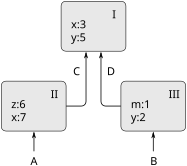
\includegraphics[width=48mm]{assets/figures/chapter_3/figure_3.1.pdf}
\end{imageFigure}

The environment is crucial to the evaluation process, because it determines the
context in which an expression should be evaluated.  Indeed, one could say that
expressions in a programming language do not, in themselves, have any meaning.
Rather, an expression acquires a meaning only with respect to some environment
in which it is evaluated.  Even the interpretation of an expression as
straightforward as \code{(+ 1 1)} depends on an understanding that one is
operating in a context in which \code{+} is the symbol for addition.  Thus, in
our model of evaluation we will always speak of evaluating an expression with
respect to some environment.  To describe interactions with the interpreter, we
will suppose that there is a global environment, consisting of a single frame
(with no enclosing environment) that includes values for the symbols associated
with the primitive procedures.  For example, the idea that \code{+} is the
symbol for addition is captured by saying that the symbol \code{+} is bound in
the global environment to the primitive addition procedure.



\subsection{The Rules for Evaluation}
\label{Section 3.2.1}

The overall specification of how the interpreter evaluates a combination
remains the same as when we first introduced it in \link{Section 1.1.3}:

\begin{itemize}
\item
To evaluate a combination:

\begin{enumerate}
\item
Evaluate the subexpressions of the combination.\footnote{Assignment introduces a
subtlety into step 1 of the evaluation rule.  As shown in \link{Exercise 3.8},
the presence of assignment allows us to write expressions that will produce
different values depending on the order in which the subexpressions in a
combination are evaluated.  Thus, to be precise, we should specify an
evaluation order in step 1 (e.g., left to right or right to left).  However,
this order should always be considered to be an implementation detail, and one
should never write programs that depend on some particular order.  For
instance, a sophisticated compiler might optimize a program by varying the
order in which subexpressions are evaluated.}

\item
Apply the value of the operator subexpression to the values of the operand
subexpressions.

\end{enumerate}
\end{itemize}

\noindent
The environment model of evaluation replaces the substitution model in
specifying what it means to apply a compound procedure to arguments.

In the environment model of evaluation, a procedure is always a pair consisting
of some code and a pointer to an environment.  Procedures are created in one
way only: by evaluating a λ-expression.  This produces a procedure
whose code is obtained from the text of the λ-expression and whose
environment is the environment in which the λ-expression was
evaluated to produce the procedure.  For example, consider the procedure
definition

\begin{codeBlock}
(define (square x)
  (* x x))
\end{codeBlock}

\noindent
evaluated in the global environment.  The procedure definition syntax is just
syntactic sugar for an underlying implicit λ-expression.  It would
have been equivalent to have used

\begin{codeBlock}
(define square
  (lambda (x) (* x x)))
\end{codeBlock}

\noindent
which evaluates \code{(lambda (x) (* x x))} and binds \code{square} to the
resulting value, all in the global environment.

\link{Figure 3.2} shows the result of evaluating this \code{define} expression.
The procedure object is a pair whose code specifies that the procedure has one
formal parameter, namely \code{x}, and a procedure body \code{(* x x)}.  The
environment part of the procedure is a pointer to the global environment, since
that is the environment in which the λ-expression was evaluated to
produce the procedure. A new binding, which associates the procedure object
with the symbol \code{square}, has been added to the global frame.  In general,
\code{define} creates definitions by adding bindings to frames.

% figure 3.2
\begin{imageFigure}
  {%
    Environment structure produced by evaluating \\
    \code{(define (square x) (* x x))} in the global environment.
  }%
  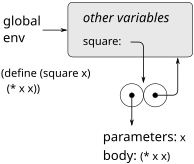
\includegraphics[width=49mm]{assets/figures/chapter_3/figure_3.2b.pdf}
\end{imageFigure}

Now that we have seen how procedures are created, we can describe how
procedures are applied.  The environment model specifies: To apply a procedure
to arguments, create a new environment containing a frame that binds the
parameters to the values of the arguments.  The enclosing environment of this
frame is the environment specified by the procedure.  Now, within this new
environment, evaluate the procedure body.

To show how this rule is followed, \link{Figure 3.3} illustrates the environment
structure created by evaluating the expression \code{(square 5)} in the global
environment, where \code{square} is the procedure generated in \link{Figure 3.2}.
Applying the procedure results in the creation of a new environment,
labeled E1 in the figure, that begins with a frame in which \code{x}, the
formal parameter for the procedure, is bound to the argument 5.  The pointer
leading upward from this frame shows that the frame's enclosing environment is
the global environment.  The global environment is chosen here, because this is
the environment that is indicated as part of the \code{square} procedure
object.  Within E1, we evaluate the body of the procedure, \code{(* x x)}.
Since the value of \code{x} in E1 is 5, the result is \code{(* 5 5)}, or 25.

% figure 3.3
\begin{imageFigure}
  {%
    Environment created by evaluating \code{(square 5)} in the global
    environment.
  }%
  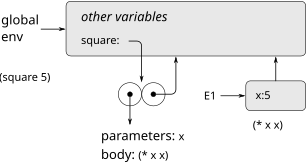
\includegraphics[width=78mm]{assets/figures/chapter_3/figure_3.3b.pdf}
\end{imageFigure}

The environment model of procedure application can be summarized by two rules:

\begin{itemize}
\item
A procedure object is applied to a set of arguments by constructing a frame,
binding the formal parameters of the procedure to the arguments of the call,
and then evaluating the body of the procedure in the context of the new
environment constructed.  The new frame has as its enclosing environment the
environment part of the procedure object being applied.

\item
A procedure is created by evaluating a λ-expression relative to a
given environment.  The resulting procedure object is a pair consisting of the
text of the λ-expression and a pointer to the environment in which
the procedure was created.
\end{itemize}

\noindent
We also specify that defining a symbol using \code{define} creates a binding in
the current environment frame and assigns to the symbol the indicated
value.\footnote{If there is already a binding for the variable in the current
frame, then the binding is changed.  This is convenient because it allows
redefinition of symbols; however, it also means that \code{define} can be used
to change values, and this brings up the issues of assignment without
explicitly using \code{set!}.  Because of this, some people prefer
redefinitions of existing symbols to signal errors or warnings.} Finally, we
specify the behavior of \code{set!}, the operation that forced us to introduce
the environment model in the first place.  Evaluating the expression
\code{(set!}\( \;\langle \)\var{variable}\( \kern0.08em\rangle \)\( \;\langle \)\var{value}\( \kern0.08em\rangle \)\code{)} in some environment locates the
binding of the variable in the environment and changes that binding to indicate
the new value.  That is, one finds the first frame in the environment that
contains a binding for the variable and modifies that frame.  If the variable
is unbound in the environment, then \code{set!} signals an error.

These evaluation rules, though considerably more complex than the substitution
model, are still reasonably straightforward.  Moreover, the evaluation model,
though abstract, provides a correct description of how the interpreter
evaluates expressions.  In \link{Chapter 4} we shall see how this model can
serve as a blueprint for implementing a working interpreter.  The following
sections elaborate the details of the model by analyzing some illustrative
programs.

\subsection{Applying Simple Procedures}
\label{Section 3.2.2}

When we introduced the substitution model in \link{Section 1.1.5} we showed how
the combination \code{(f 5)} evaluates to 136, given the following procedure
definitions:

\begin{codeBlock}
(define (square x)
  (* x x))
(define (sum-of-squares x y)
  (+ (square x) (square y)))
(define (f a)
  (sum-of-squares (+ a 1) (* a 2)))
\end{codeBlock}

\noindent
We can analyze the same example using the environment model.  \link{Figure 3.4}
shows the three procedure objects created by evaluating the definitions of
\code{f}, \code{square}, and \code{sum\-/of\-/squares} in the global environment.
Each procedure object consists of some code, together with a pointer to the
global environment.

% figure 3.4
\begin{imageFigure}{Procedure objects in the global frame.}
  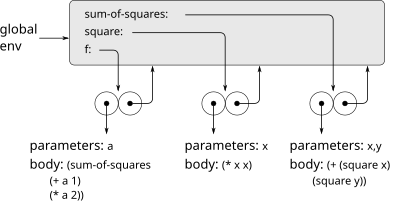
\includegraphics[width=106mm]{assets/figures/chapter_3/figure_3.4a.pdf}
\end{imageFigure}

In \link{Figure 3.5} we see the environment structure created by evaluating the
expression \code{(f 5)}.  The call to \code{f} creates a new environment E1
beginning with a frame in which \code{a}, the formal parameter of \code{f}, is
bound to the argument 5.  In E1, we evaluate the body of \code{f}:

\begin{codeBlock}
(sum-of-squares (+ a 1) (* a 2))
\end{codeBlock}

\noindent
To evaluate this combination, we first evaluate the subexpressions.  The first
subexpression, \code{sum\-/of\-/squares}, has a value that is a procedure object.
(Notice how this value is found: We first look in the first frame of E1, which
contains no binding for \code{sum\-/of\-/squares}.  Then we proceed to the
enclosing environment, i.e. the global environment, and find the binding shown
in \link{Figure 3.4}.)  The other two subexpressions are evaluated by applying
the primitive operations \code{+} and \code{*} to evaluate the two combinations
\code{(+ a 1)} and \code{(* a 2)} to obtain 6 and 10, respectively.

Now we apply the procedure object \code{sum\-/of\-/squares} to the arguments 6 and
10.  This results in a new environment E2 in which the formal parameters
\code{x} and \code{y} are bound to the arguments.  Within E2 we evaluate the
combination \code{(+ (square x) (square y))}.  This leads us to evaluate
\code{(square x)}, where \code{square} is found in the global frame and
\code{x} is 6.  Once again, we set up a new environment, E3, in which \code{x}
is bound to 6, and within this we evaluate the body of \code{square}, which is
\code{(* x x)}.  Also as part of applying \code{sum\-/of\-/squares}, we must
evaluate the subexpression \code{(square y)}, where \code{y} is 10.  This
second call to \code{square} creates another environment, E4, in which
\code{x}, the formal parameter of \code{square}, is bound to 10.  And within E4
we must evaluate \code{(* x x)}.

% figure 3.5
\begin{imageFigure}
  {%
    Environments created by evaluating \code{(f 5)} using the procedures in
    \link{Figure 3.4}.
  }%
  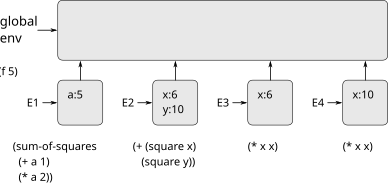
\includegraphics[width=100mm]{assets/figures/chapter_3/figure_3.5a.pdf}
\end{imageFigure}

The important point to observe is that each call to \code{square} creates a new
environment containing a binding for \code{x}.  We can see here how the
different frames serve to keep separate the different local variables all named
\code{x}.  Notice that each frame created by \code{square} points to the global
environment, since this is the environment indicated by the \code{square}
procedure object.

After the subexpressions are evaluated, the results are returned.  The values
generated by the two calls to \code{square} are added by \code{sum\-/of\-/squares},
and this result is returned by \code{f}.  Since our focus here is on the
environment structures, we will not dwell on how these returned values are
passed from call to call; however, this is also an important aspect of the
evaluation process, and we will return to it in detail in \link{Chapter 5}.

\begin{exerciseGroup}
\phantomsection\label{Exercise 3.9}
\exerciseHeading{Exercise 3.9:} In \link{Section 1.2.1} we used the
substitution model to analyze two procedures for computing factorials, a
recursive version

\begin{codeBlock}
(define (factorial n)
  (if (= n 1) 1 (* n (factorial (- n 1)))))
\end{codeBlock}

\noindent
and an iterative version

\begin{codeBlock}
(define (factorial n) (fact-iter 1 1 n))
(define (fact-iter product counter max-count)
  (if (> counter max-count)
      product
      (fact-iter (* counter product)
                 (+ counter 1)
                 max-count)))
\end{codeBlock}

Show the environment structures created by evaluating \\ \code{(factorial 6)}
using each version of the \code{factorial} procedure.\footnote{The environment
model will not clarify our claim in \link{Section 1.2.1} that the interpreter
can execute a procedure such as \code{fact\-/iter} in a constant amount of space
using tail recursion.  We will discuss tail recursion when we deal with the
control structure of the interpreter in \link{Section 5.4}.}
\end{exerciseGroup}

\subsection{Frames as the Repository of Local State}
\label{Section 3.2.3}

We can turn to the environment model to see how procedures and assignment can
be used to represent objects with local state.  As an example, consider the
``withdrawal processor'' from \link{Section 3.1.1} created by calling the
procedure

\begin{codeBlock}
(define (make-withdraw balance)
  (lambda (amount)
    (if (>= balance amount)
        (begin (set! balance (- balance amount))
               balance)
        "Insufficient funds")))
\end{codeBlock}

\noindent
Let us describe the evaluation of

\begin{codeBlock}
(define W1 (make-withdraw 100))
\end{codeBlock}

\noindent
followed by

\begin{codeBlock}
(W1 50)
~\textit{50}~
\end{codeBlock}

\noindent
\link{Figure 3.6} shows the result of defining the \code{make\-/withdraw}
procedure in the global environment.  This produces a procedure object that
contains a pointer to the global environment.  So far, this is no different
from the examples we have already seen, except that the body of the procedure
is itself a λ-expression.

% figure 3.6
\begin{imageFigure}
  {Result of defining \code{make\-/withdraw} in the global environment.}
  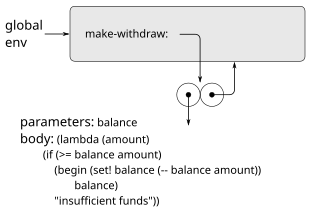
\includegraphics[width=91mm]{assets/figures/chapter_3/figure_3.6b.pdf}
\end{imageFigure}

% figure 3.7
\begin{imageFigure}
  {Result of evaluating \code{(define W1 (make\-/withdraw 100))}.}
  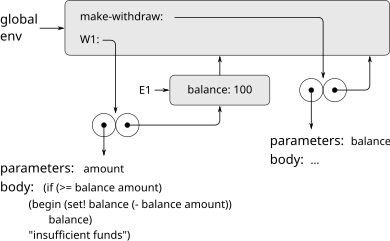
\includegraphics[width=100mm]{assets/figures/chapter_3/figure_3.7a.pdf}
\end{imageFigure}

The interesting part of the computation happens when we apply the procedure
\code{make\-/withdraw} to an argument:

\begin{codeBlock}
(define W1 (make-withdraw 100))
\end{codeBlock}

\noindent
We begin, as usual, by setting up an environment E1 in which the formal
parameter \code{balance} is bound to the argument 100.  Within this
environment, we evaluate the body of \code{make\-/withdraw}, namely the
λ-expression.  This constructs a new procedure object, whose code
is as specified by the \code{lambda} and whose environment is E1, the
environment in which the \code{lambda} was evaluated to produce the procedure.
The resulting procedure object is the value returned by the call to
\code{make\-/withdraw}.  This is bound to \code{W1} in the global environment,
since the \code{define} itself is being evaluated in the global environment.
\link{Figure 3.7} shows the resulting environment structure.

% figure 3.8
\begin{imageFigure}
  {Environments created by applying the procedure object \code{W1}.}
  \includegraphics[width=99mm]{assets/figures/chapter_3/figure_3.8c.pdf}
\end{imageFigure}

Now we can analyze what happens when \code{W1} is applied to an argument:

\begin{codeBlock}
(W1 50)
~\textit{50}~
\end{codeBlock}

We begin by constructing a frame in which \code{amount}, the formal parameter
of \code{W1}, is bound to the argument 50.  The crucial point to observe is
that this frame has as its enclosing environment not the global environment,
but rather the environment E1, because this is the environment that is
specified by the \code{W1} procedure object.  Within this new environment, we
evaluate the body of the procedure:

\begin{codeBlock}
(if (>= balance amount)
    (begin (set! balance (- balance amount))
           balance)
    "Insufficient funds")
\end{codeBlock}

\noindent
The resulting environment structure is shown in \link{Figure 3.8}.  The
expression being evaluated references both \code{amount} and \code{balance}.
\code{amount} will be found in the first frame in the environment, while
\code{balance} will be found by following the enclosing-environment pointer to
E1.

% figure 3.9
\begin{imageFigure}{Environments after the call to \code{W1}.}
  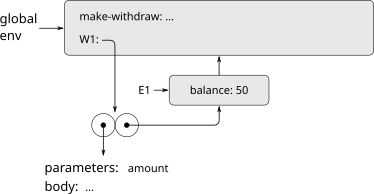
\includegraphics[width=96mm]{assets/figures/chapter_3/figure_3.9a.pdf}
\end{imageFigure}

When the \code{set!} is executed, the binding of \code{balance} in E1 is
changed.  At the completion of the call to \code{W1}, \code{balance} is 50, and
the frame that contains \code{balance} is still pointed to by the procedure
object \code{W1}.  The frame that binds \code{amount} (in which we executed the
code that changed \code{balance}) is no longer relevant, since the procedure
call that constructed it has terminated, and there are no pointers to that
frame from other parts of the environment.  The next time \code{W1} is called,
this will build a new frame that binds \code{amount} and whose enclosing
environment is E1.  We see that E1 serves as the ``place'' that holds the local
state variable for the procedure object \code{W1}.  \link{Figure 3.9} shows the
situation after the call to \code{W1}.

Observe what happens when we create a second ``withdraw'' object by making
another call to \code{make\-/withdraw}:

\begin{codeBlock}
(define W2 (make-withdraw 100))
\end{codeBlock}

% figure 3.10
\begin{imageFigure}
  {Using \code{(define W2 (make\-/withdraw 100))} to create a second object.}
  \includegraphics[width=108mm]{assets/figures/chapter_3/figure_3.10a.pdf}
\end{imageFigure}

This produces the environment structure of \link{Figure 3.10}, which shows that
\code{W2} is a procedure object, that is, a pair with some code and an
environment.  The environment E2 for \code{W2} was created by the call to
\code{make\-/withdraw}.  It contains a frame with its own local binding for
\code{balance}.  On the other hand, \code{W1} and \code{W2} have the same code:
the code specified by the λ-expression in the body of
\code{make\-/withdraw}.\footnote{Whether \code{W1} and \code{W2} share the same
physical code stored in the computer, or whether they each keep a copy of the
code, is a detail of the implementation.  For the interpreter we implement in
\link{Chapter 4}, the code is in fact shared.} We see here why \code{W1} and
\code{W2} behave as independent objects.  Calls to \code{W1} reference the
state variable \code{balance} stored in E1, whereas calls to \code{W2}
reference the \code{balance} stored in E2. Thus, changes to the local state of
one object do not affect the other object.

\begin{exerciseGroup}
\phantomsection\label{Exercise 3.10}
\exerciseHeading{Exercise 3.10:} In the \code{make\-/withdraw}
procedure, the local variable \code{balance} is created as a parameter of
\code{make\-/withdraw}.  We could also create the local state variable
explicitly, using \code{let}, as follows:

\begin{codeBlock}
(define (make-withdraw initial-amount)
  (let ((balance initial-amount))
    (lambda (amount)
      (if (>= balance amount)
          (begin (set! balance (- balance amount))
                 balance)
          "Insufficient funds"))))
\end{codeBlock}

Recall from \link{Section 1.3.2} that \code{let} is simply syntactic sugar for a
procedure call:

\begin{codeBlock}
(let ((~\(\langle \)~~\var{var}~~\(\rangle \)~ ~\(\langle \)~~\var{exp}~~\(\rangle \)~)) ~\(\langle \)~~\var{body}~~\(\rangle \)~)
\end{codeBlock}

\noindent
is interpreted as an alternate syntax for

\begin{codeBlock}
((lambda (~\(\langle \)~~\var{var}~~\(\rangle \)~) ~\(\langle \)~~\var{body}~~\(\rangle \)~) ~\(\langle \)~~\var{exp}~~\(\rangle \)~)
\end{codeBlock}

Use the environment model to analyze this alternate version of
\code{make\-/withdraw}, drawing figures like the ones above to illustrate the
interactions

\begin{codeBlock}
(define W1 (make-withdraw 100))
(W1 50)
(define W2 (make-withdraw 100))
\end{codeBlock}

Show that the two versions of \code{make\-/withdraw} create objects with the same
behavior.  How do the environment structures differ for the two versions?
\end{exerciseGroup}

\subsection{Internal Definitions}
\label{Section 3.2.4}

\link{Section 1.1.8} introduced the idea that procedures can have internal
definitions, thus leading to a block structure as in the following procedure to
compute square roots:

\begin{codeBlock}
(define (sqrt x)
  (define (good-enough? guess)
    (< (abs (- (square guess) x)) 0.001))
  (define (improve guess)
    (average guess (/ x guess)))
  (define (sqrt-iter guess)
    (if (good-enough? guess)
        guess
        (sqrt-iter (improve guess))))
  (sqrt-iter 1.0))
\end{codeBlock}

\noindent
Now we can use the environment model to see why these internal definitions
behave as desired.  \link{Figure 3.11} shows the point in the evaluation of the
expression \code{(sqrt 2)} where the internal procedure \code{good\-/enough?} has
been called for the first time with \code{guess} equal to 1.

Observe the structure of the environment.  \code{sqrt} is a symbol in the
global environment that is bound to a procedure object whose associated
environment is the global environment.  When \code{sqrt} was called, a new
environment E1 was formed, subordinate to the global environment, in which the
parameter \code{x} is bound to 2.  The body of \code{sqrt} was then evaluated
in E1.  Since the first expression in the body of \code{sqrt} is

\begin{codeBlock}
(define (good-enough? guess)
  (< (abs (- (square guess) x)) 0.001))
\end{codeBlock}

\noindent
evaluating this expression defined the procedure \code{good\-/enough?}  in the
environment E1.  To be more precise, the symbol \code{good\-/enough?} was added
to the first frame of E1, bound to a procedure object whose associated
environment is E1.  Similarly, \code{improve} and \code{sqrt\-/iter} were defined
as procedures in E1.  For conciseness, \link{Figure 3.11} shows only the
procedure object for \code{good\-/enough?}.

% figure 3.11
\begin{imageFigure}{\code{sqrt} procedure with internal definitions.}
  \includegraphics[width=107mm]{assets/figures/chapter_3/figure_3.11a.pdf}
\end{imageFigure}

After the local procedures were defined, the expression \code{(sqrt\-/iter 1.0)}
was evaluated, still in environment E1.  So the procedure object bound to
\code{sqrt\-/iter} in E1 was called with 1 as an argument.  This created an
environment E2 in which \code{guess}, the parameter of \code{sqrt\-/iter}, is
bound to 1.  \code{sqrt\-/iter} in turn called \code{good\-/enough?} with the value
of \code{guess} (from E2) as the argument for \code{good\-/enough?}.  This set up
another environment, E3, in which \code{guess} (the parameter of
\code{good\-/enough?}) is bound to 1.  Although \code{sqrt\-/iter} and
\code{good\-/enough?} both have a parameter named \code{guess}, these are two
distinct local variables located in different frames.  Also, E2 and E3 both
have E1 as their enclosing environment, because the \code{sqrt\-/iter} and
\code{good\-/enough?} procedures both have E1 as their environment part.  One
consequence of this is that the symbol \code{x} that appears in the body of
\code{good\-/enough?} will reference the binding of \code{x} that appears in E1,
namely the value of \code{x} with which the original \code{sqrt} procedure was
called.

The environment model thus explains the two key properties that make local
procedure definitions a useful technique for modularizing programs:

\begin{itemize}
\item
The names of the local procedures do not interfere with names external to the
enclosing procedure, because the local procedure names will be bound in the
frame that the procedure creates when it is run, rather than being bound in the
global environment.

\item
The local procedures can access the arguments of the enclosing procedure,
simply by using parameter names as free variables.  This is because the body of
the local procedure is evaluated in an environment that is subordinate to the
evaluation environment for the enclosing procedure.
\end{itemize}

\begin{exerciseGroup}
\phantomsection\label{Exercise 3.11}
\exerciseHeading{Exercise 3.11:} In \link{Section 3.2.3} we saw how
the environment model described the behavior of procedures with local state.
Now we have seen how internal definitions work.  A typical message-passing
procedure contains both of these aspects.  Consider the bank account procedure
of \link{Section 3.1.1}:

\begin{codeBlock}
(define (make-account balance)
  (define (withdraw amount)
    (if (>= balance amount)
        (begin (set! balance (- balance amount))
               balance)
        "Insufficient funds"))
  (define (deposit amount)
    (set! balance (+ balance amount))
    balance)
  (define (dispatch m)
    (cond ((eq? m 'withdraw) withdraw)
          ((eq? m 'deposit) deposit)
          (else
           (error "Unknown request: MAKE-ACCOUNT"
                  m))))
  dispatch)
\end{codeBlock}

Show the environment structure generated by the sequence of interactions

\begin{codeBlock}
(define acc (make-account 50))
((acc 'deposit) 40)
~\textit{90}~
((acc 'withdraw) 60)
~\textit{30}~
\end{codeBlock}

Where is the local state for \code{acc} kept?  Suppose we define another
account

\begin{codeBlock}
(define acc2 (make-account 100))
\end{codeBlock}

How are the local states for the two accounts kept distinct?  Which parts of
the environment structure are shared between \code{acc} and \code{acc2}?
\end{exerciseGroup}

\section{Modeling with Mutable Data}
\label{Section 3.3}

Chapter 2 dealt with compound data as a means for constructing computational
objects that have several parts, in order to model real-world objects that have
several aspects.  In that chapter we introduced the discipline of data
abstraction, according to which data structures are specified in terms of
constructors, which create data objects, and selectors, which access the parts
of compound data objects.  But we now know that there is another aspect of data
that \link{Chapter 2} did not address.  The desire to model systems composed of
objects that have changing state leads us to the need to modify compound data
objects, as well as to construct and select from them.  In order to model
compound objects with changing state, we will design data abstractions to
include, in addition to selectors and constructors, operations called
\newterm{mutators}, which modify data objects.  For instance, modeling a
banking system requires us to change account balances.  Thus, a data structure
for representing bank accounts might admit an operation

\begin{codeBlock}
(set-balance! ~\(\langle \)~~\var{account}~~\(\rangle \)~ ~\(\langle \)~~\var{new-value}~~\(\rangle \)~)
\end{codeBlock}

\noindent
that changes the balance of the designated account to the designated new value.
Data objects for which mutators are defined are known as \newterm{mutable data
objects}.

\link{Chapter 2} introduced pairs as a general-purpose ``glue'' for synthesizing
compound data.  We begin this section by defining basic mutators for pairs, so
that pairs can serve as building blocks for constructing mutable data objects.
These mutators greatly enhance the representational power of pairs, enabling us
to build data structures other than the sequences and trees that we worked with
in \link{Section 2.2}.  We also present some examples of simulations in which
complex systems are modeled as collections of objects with local state.



\subsection{Mutable List Structure}
\label{Section 3.3.1}

The basic operations on pairs---\code{cons}, \code{car}, and \code{cdr}---can
be used to construct list structure and to select parts from list structure,
but they are incapable of modifying list structure.  The same is true of the
list operations we have used so far, such as \code{append} and \code{list},
since these can be defined in terms of \code{cons}, \code{car}, and \code{cdr}.
To modify list structures we need new operations.

The primitive mutators for pairs are \code{set\-/car!} and
\code{set\-/cdr!}. \code{set\-/car!} takes two arguments, the first of which must
be a pair.  It modifies this pair, replacing the \code{car} pointer by a
pointer to the second argument of \code{set\-/car!}.\footnote{\code{set\-/car!} and
\code{set\-/cdr!} return implementation-dependent values.  Like \code{set!}, they
should be used only for their effect.}

As an example, suppose that \code{x} is bound to the list \code{((a b) c d)}
and \code{y} to the list \code{(e f)} as illustrated in \link{Figure 3.12}.
Evaluating the expression \code{ (set\-/car!  x y)} modifies the pair to which
\code{x} is bound, replacing its \code{car} by the value of \code{y}.  The
result of the operation is shown in \link{Figure 3.13}.  The structure \code{x}
has been modified and would now be printed as \code{((e f) c d)}.  The pairs
representing the list \code{(a b)}, identified by the pointer that was
replaced, are now detached from the original structure.\footnote{We see from
this that mutation operations on lists can create ``garbage'' that is not part
of any accessible structure.  We will see in \link{Section 5.3.2} that Lisp
memory-management systems include a \newterm{garbage collector}, which
identifies and recycles the memory space used by unneeded pairs.}

Compare \link{Figure 3.13} with \link{Figure 3.14}, which illustrates the result
of executing \code{(define z (cons y (cdr x)))} with \code{x} and \code{y}
bound to the original lists of \link{Figure 3.12}.  The variable \code{z} is now
bound to a new pair created by the \code{cons} operation; the list to which
\code{x} is bound is unchanged.

% figure 3.12
\begin{imageFigure}
  {Lists \code{x}: \code{((a b) c d)} and \code{y}: \code{(e f)}.}
  \includegraphics[width=72mm]{assets/figures/chapter_3/figure_3.12b.pdf}
\end{imageFigure}

% figure 3.13
\begin{imageFigure}
  {Effect of \code{(set\-/car! x y)} on the lists in \link{Figure 3.12}.}
  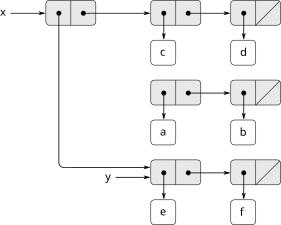
\includegraphics[width=72mm]{assets/figures/chapter_3/figure_3.13b.pdf}
\end{imageFigure}

% figure 3.14
\begin{imageFigure}
  {%
    Effect of \code{(define z (cons y (cdr x)))} on the lists in
    \link{Figure 3.12}.
  }%
  \includegraphics[width=72mm]{assets/figures/chapter_3/figure_3.14b.pdf}
\end{imageFigure}

% figure 3.15
\begin{imageFigure}
  {Effect of \code{(set\-/cdr! x y)} on the lists in \link{Figure 3.12}.}
  \includegraphics[width=72mm]{assets/figures/chapter_3/figure_3.15b.pdf}
\end{imageFigure}

The \code{set\-/cdr!} operation is similar to \code{set\-/car!}.  The only
difference is that the \code{cdr} pointer of the pair, rather than the
\code{car} pointer, is replaced.  The effect of executing \code{(set\-/cdr! x y)}
on the lists of \link{Figure 3.12} is shown in \link{Figure 3.15}.  Here the
\code{cdr} pointer of \code{x} has been replaced by the pointer to \code{(e
f)}.  Also, the list \code{(c d)}, which used to be the \code{cdr} of \code{x},
is now detached from the structure.

\begin{codeBlock}
(define (cons x y)
  (let ((new (get-new-pair)))
    (set-car! new x)
    (set-cdr! new y)
    new))
\end{codeBlock}

\code{cons} builds new list structure by creating new pairs, while
\code{set\-/car!} and \code{set\-/cdr!} modify existing pairs.  Indeed, we could
implement \code{cons} in terms of the two mutators, together with a procedure
\code{get\-/new\-/pair}, which returns a new pair that is not part of any existing
list structure.  We obtain the new pair, set its \code{car} and \code{cdr}
pointers to the designated objects, and return the new pair as the result of
the \code{cons}.\footnote{\code{get\-/new\-/pair} is one of the operations that
must be implemented as part of the memory management required by a Lisp
implementation.  We will discuss this in \link{Section 5.3.1}.}

\begin{exerciseGroup}
\phantomsection\label{Exercise 3.12}
\exerciseHeading{Exercise 3.12:} The following procedure for
appending lists was introduced in \link{Section 2.2.1}:

\begin{codeBlock}
(define (append x y)
  (if (null? x)
      y
      (cons (car x) (append (cdr x) y))))
\end{codeBlock}

\code{append} forms a new list by successively \code{cons}ing the elements of
\code{x} onto \code{y}.  The procedure \code{append!} is similar to
\code{append}, but it is a mutator rather than a constructor.  It appends the
lists by splicing them together, modifying the final pair of \code{x} so that
its \code{cdr} is now \code{y}.  (It is an error to call \code{append!} with an
empty \code{x}.)

\begin{codeBlock}
(define (append! x y)
  (set-cdr! (last-pair x) y)
  x)
\end{codeBlock}

Here \code{last\-/pair} is a procedure that returns the last pair in its
argument:

\begin{codeBlock}
(define (last-pair x)
  (if (null? (cdr x)) x (last-pair (cdr x))))
\end{codeBlock}

Consider the interaction

\begin{codeBlock}
(define x (list 'a 'b))
(define y (list 'c 'd))
(define z (append x y))
z
~\textit{(a b c d)}~
(cdr x)
~\(\langle \)~~\var{response}~~\(\rangle \)~
(define w (append! x y))
w
~\textit{(a b c d)}~
(cdr x)
~\(\langle \)~~\var{response}~~\(\rangle \)~
\end{codeBlock}

What are the missing \( \langle \)\var{response}\( \rangle \)s?
Draw box-and-pointer \\ diagrams to explain your answer.

\phantomsection\label{Exercise 3.13}
\exerciseHeading{Exercise 3.13:} Consider the following
\code{make\-/cycle} procedure, which uses the \code{last\-/pair} procedure defined
in \link{Exercise 3.12}:

\begin{codeBlock}
(define (make-cycle x)
  (set-cdr! (last-pair x) x)
  x)
\end{codeBlock}

Draw a box-and-pointer diagram that shows the structure \code{z} created by

\begin{codeBlock}
(define z (make-cycle (list 'a 'b 'c)))
\end{codeBlock}

What happens if we try to compute \code{(last\-/pair z)}?

\phantomsection\label{Exercise 3.14}
\exerciseHeading{Exercise 3.14:} The following procedure is quite
useful, although obscure:

\begin{codeBlock}
(define (mystery x)
  (define (loop x y)
    (if (null? x)
        y
        (let ((temp (cdr x)))
          (set-cdr! x y)
          (loop temp x))))
  (loop x '()))
\end{codeBlock}

\code{loop} uses the ``temporary'' variable \code{temp} to hold the old value
of the \code{cdr} of \code{x}, since the \code{set\-/cdr!}  on the next line
destroys the \code{cdr}.  Explain what \code{mystery} does in general.  Suppose
\code{v} is defined by \code{(define v (list 'a 'b 'c 'd))}. Draw the
box-and-pointer diagram that represents the list to which \code{v} is bound.
Suppose that we now evaluate \code{(define w (mystery v))}. Draw
box-and-pointer diagrams that show the structures \code{v} and \code{w} after
evaluating this expression.  What would be printed as the values of \code{v}
and \code{w}?
\end{exerciseGroup}

\subsubsection*{Sharing and identity}

We mentioned in \link{Section 3.1.3} the theoretical issues of ``sameness'' and
``change'' raised by the introduction of assignment.  These issues arise in
practice when individual pairs are \newterm{shared} among different data
objects.  For example, consider the structure formed by

\begin{codeBlock}
(define x (list 'a 'b))
(define z1 (cons x x))
\end{codeBlock}

\noindent
As shown in \link{Figure 3.16}, \code{z1} is a pair whose \code{car} and
\code{cdr} both point to the same pair \code{x}.  This sharing of \code{x} by
the \code{car} and \code{cdr} of \code{z1} is a consequence of the
straightforward way in which \code{cons} is implemented.  In general, using
\code{cons} to construct lists will result in an interlinked structure of pairs
in which many individual pairs are shared by many different structures.

In contrast to \link{Figure 3.16}, \link{Figure 3.17} shows the structure created
by

\begin{codeBlock}
(define z2 (cons (list 'a 'b) (list 'a 'b)))
\end{codeBlock}

\noindent
In this structure, the pairs in the two \code{(a b)} lists are distinct,
although the actual symbols are shared.\footnote{The two pairs are distinct
because each call to \code{cons} returns a new pair.  The symbols are shared;
in Scheme there is a unique symbol with any given name.  Since Scheme provides
no way to mutate a symbol, this sharing is undetectable.  Note also that the
sharing is what enables us to compare symbols using \code{eq?}, which simply
checks equality of pointers.}

% figure 3.16
\begin{imageFigure}
  {The list \code{z1} formed by \code{(cons x x)}.}
  \includegraphics[width=46mm]{assets/figures/chapter_3/figure_3.16b.pdf}
\end{imageFigure}

% figure 3.17
\begin{imageFigure}
  {The list \code{z2} formed by \code{(cons (list 'a 'b) (list 'a 'b))}.}
  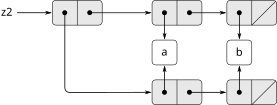
\includegraphics[width=71mm]{assets/figures/chapter_3/figure_3.17b.pdf}
\end{imageFigure}

When thought of as a list, \code{z1} and \code{z2} both represent ``the same''
list, \code{((a b) a b)}.  In general, sharing is completely undetectable if we
operate on lists using only \code{cons}, \code{car}, and \code{cdr}.  However,
if we allow mutators on list structure, sharing becomes significant.  As an
example of the difference that sharing can make, consider the following
procedure, which modifies the \code{car} of the structure to which it is
applied:

\begin{codeBlock}
(define (set-to-wow! x) (set-car! (car x) 'wow) x)
\end{codeBlock}

\noindent
Even though \code{z1} and \code{z2} are ``the same'' structure, applying
\code{set\-/to\-/wow!} to them yields different results.  With \code{z1}, altering
the \code{car} also changes the \code{cdr}, because in \code{z1} the \code{car}
and the \code{cdr} are the same pair.  With \code{z2}, the \code{car} and
\code{cdr} are distinct, so \code{set\-/to\-/wow!} modifies only the \code{car}:

\begin{codeBlock}
z1
~\textit{((a b) a b)}~
(set-to-wow! z1)
~\textit{((wow b) wow b)}~
z2
~\textit{((a b) a b)}~
(set-to-wow! z2)
~\textit{((wow b) a b)}~
\end{codeBlock}

\noindent
One way to detect sharing in list structures is to use the predicate
\code{eq?}, which we introduced in \link{Section 2.3.1} as a way to test whether
two symbols are equal.  More generally, \code{(eq?  x y)} tests whether
\code{x} and \code{y} are the same object (that is, whether \code{x} and
\code{y} are equal as pointers).  Thus, with \code{z1} and \code{z2} as defined
in \link{Figure 3.16} and \link{Figure 3.17}, \code{(eq?  (car z1) (cdr
z1))} is true and \code{(eq? (car z2) (cdr z2))} is false.

As will be seen in the following sections, we can exploit sharing to greatly
extend the repertoire of data structures that can be represented by pairs.  On
the other hand, sharing can also be dangerous, since modifications made to
structures will also affect other structures that happen to share the modified
parts.  The mutation operations \code{set\-/car!} and \code{set\-/cdr!} should be
used with care; unless we have a good understanding of how our data objects are
shared, mutation can have unanticipated results.\footnote{The subtleties of
dealing with sharing of mutable data objects reflect the underlying issues of
``sameness'' and ``change'' that were raised in \link{Section 3.1.3}.  We
mentioned there that admitting change to our language requires that a compound
object must have an ``identity'' that is something different from the pieces
from which it is composed.  In Lisp, we consider this ``identity'' to be the
quality that is tested by \code{eq?}, i.e., by equality of pointers.  Since in
most Lisp implementations a pointer is essentially a memory address, we are
``solving the problem'' of defining the identity of objects by stipulating that
a data object ``itself\( \kern0.1em \)'' is the information stored in some particular set of
memory locations in the computer.  This suffices for simple Lisp programs, but
is hardly a general way to resolve the issue of ``sameness'' in computational
models.}

\begin{exerciseGroup}
\phantomsection\label{Exercise 3.15}
\exerciseHeading{Exercise 3.15:} Draw box-and-pointer diagrams to
explain the effect of \code{set\-/to\-/wow!} on the structures \code{z1} and
\code{z2} above.

\phantomsection\label{Exercise 3.16}
\exerciseHeading{Exercise 3.16:} Ben Bitdiddle decides to write a
procedure to count the number of pairs in any list structure.  ``It's easy,''
he reasons.  ``The number of pairs in any structure is the number in the
\code{car} plus the number in the \code{cdr} plus one more to count the current
pair.''  So Ben writes the following procedure:

\begin{codeBlock}
(define (count-pairs x)
  (if (not (pair? x))
      0
      (+ (count-pairs (car x))
         (count-pairs (cdr x))
         1)))
\end{codeBlock}

Show that this procedure is not correct.  In particular, draw box-and-pointer
diagrams representing list structures made up of exactly three pairs for which
Ben's procedure would return 3; return 4; return 7; never return at all.

\phantomsection\label{Exercise 3.17}
\exerciseHeading{Exercise 3.17:} Devise a correct version of the
\code{count\-/pairs} procedure of \link{Exercise 3.16} that returns the number of
distinct pairs in any structure.  (Hint: Traverse the structure, maintaining an
auxiliary data structure that is used to keep track of which pairs have already
been counted.)

\phantomsection\label{Exercise 3.18}
\exerciseHeading{Exercise 3.18:} Write a procedure that examines a
list and determines whether it contains a cycle, that is, whether a program
that tried to find the end of the list by taking successive \code{cdr}s would
go into an infinite loop.  \link{Exercise 3.13} constructed such lists.

\phantomsection\label{Exercise 3.19}
\exerciseHeading{Exercise 3.19:} Redo \link{Exercise 3.18} using an
algorithm that takes only a constant amount of space.  (This requires a very
clever idea.)
\end{exerciseGroup}

\subsubsection*{Mutation is just assignment}

When we introduced compound data, we observed in \link{Section 2.1.3} that pairs
can be represented purely in terms of procedures:

\begin{codeBlock}
(define (cons x y)
  (define (dispatch m)
    (cond ((eq? m 'car) x)
          ((eq? m 'cdr) y)
          (else (error "Undefined operation: CONS" m))))
  dispatch)
(define (car z) (z 'car))
(define (cdr z) (z 'cdr))
\end{codeBlock}

\noindent
The same observation is true for mutable data.  We can implement mutable data
objects as procedures using assignment and local state.  For instance, we can
extend the above pair implementation to handle \code{set\-/car!} and
\code{set\-/cdr!} in a manner analogous to the way we implemented bank accounts
using \code{make\-/account} in \link{Section 3.1.1}:

\begin{codeBlock}
(define (cons x y)
  (define (set-x! v) (set! x v))
  (define (set-y! v) (set! y v))
  (define (dispatch m)
    (cond ((eq? m 'car) x)
          ((eq? m 'cdr) y)
          ((eq? m 'set-car!) set-x!)
          ((eq? m 'set-cdr!) set-y!)
          (else
           (error "Undefined operation: CONS" m))))
  dispatch)
(define (car z) (z 'car))
(define (cdr z) (z 'cdr))
(define (set-car! z new-value)
  ((z 'set-car!) new-value) z)
(define (set-cdr! z new-value)
  ((z 'set-cdr!) new-value) z)
\end{codeBlock}

\noindent
Assignment is all that is needed, theoretically, to account for the behavior of
mutable data.  As soon as we admit \code{set!} to our language, we raise all
the issues, not only of assignment, but of mutable data in general.\footnote{On
the other hand, from the viewpoint of implementation, assignment requires us to
modify the environment, which is itself a mutable data structure.  Thus,
assignment and mutation are equipotent: Each can be implemented in terms of the
other.}

\begin{exerciseGroup}
\phantomsection\label{Exercise 3.20}
\exerciseHeading{Exercise 3.20:} Draw environment diagrams to
illustrate the evaluation of the sequence of expressions

\begin{codeBlock}
(define x (cons 1 2))
(define z (cons x x))
(set-car! (cdr z) 17)
(car x)
~\textit{17}~
\end{codeBlock}

\noindent
using the procedural implementation of pairs given above.  (Compare
\link{Exercise 3.11}.)
\end{exerciseGroup}

\subsection{Representing Queues}
\label{Section 3.3.2}

The mutators \code{set\-/car!} and \code{set\-/cdr!} enable us to use pairs to
construct data structures that cannot be built with \code{cons}, \code{car},
and \code{cdr} alone.  This section shows how to use pairs to represent a data
structure called a queue.  \link{Section 3.3.3} will show how to represent data
structures called tables.

A \newterm{queue} is a sequence in which items are inserted at one end (called
the \newterm{rear} of the queue) and deleted from the other end (the
\newterm{front}).  \link{Figure 3.18} shows an initially empty queue in which
the items \code{a} and \code{b} are inserted.  Then \code{a} is removed,
\code{c} and \code{d} are inserted, and \code{b} is removed.  Because items are
always removed in the order in which they are inserted, a queue is sometimes
called a \newterm{FIFO} (first in, first out) buffer.

% figure 3.18
\begin{imageFigure}
  {Queue operations.}
  \includegraphics[width=70mm]{assets/figures/chapter_3/figure_3.18a.pdf}
\end{imageFigure}

In terms of data abstraction, we can regard a queue as defined by the following
set of operations:

\begin{itemize}
\item
a constructor: \code{(make\-/queue)} returns an empty queue (a queue containing
no items).

\item
two selectors:

\code{(empty\-/queue? \( \langle \)\var{queue}\( \rangle \))}
tests if the queue is empty.

\code{(front\-/queue \( \langle \)\var{queue}\( \rangle \))}
returns the object at the front of the queue, signaling an error if the queue
is empty; it does not modify the queue.

\item
two mutators:

\code{(insert\-/queue! \( \langle \)\var{queue}\( \rangle \) \( \langle \)\var{item}\( \rangle \))}
inserts the item at the rear of the queue and returns the modified queue as its
value.

\code{(delete\-/queue! \( \langle \)\var{queue}\( \rangle \))}
removes the item at the front of the queue and returns the modified queue as
its value, signaling an error if the queue is empty before the deletion.
\end{itemize}

\noindent
Because a queue is a sequence of items, we could certainly represent it as an
ordinary list; the front of the queue would be the \code{car} of the list,
inserting an item in the queue would amount to appending a new element at the
end of the list, and deleting an item from the queue would just be taking the
\code{cdr} of the list.  However, this representation is inefficient, because
in order to insert an item we must scan the list until we reach the end.  Since
the only method we have for scanning a list is by successive \code{cdr}
operations, this scanning requires \( \Theta(n) \) steps for a list of \( n \)
items.  A simple modification to the list representation overcomes this
disadvantage by allowing the queue operations to be implemented so that they
require \( \Theta \)(1) steps; that is, so that the number of steps needed is
independent of the length of the queue.

The difficulty with the list representation arises from the need to scan to
find the end of the list.  The reason we need to scan is that, although the
standard way of representing a list as a chain of pairs readily provides us
with a pointer to the beginning of the list, it gives us no easily accessible
pointer to the end.  The modification that avoids the drawback is to represent
the queue as a list, together with an additional pointer that indicates the
final pair in the list.  That way, when we go to insert an item, we can consult
the rear pointer and so avoid scanning the list.

A queue is represented, then, as a pair of pointers, \code{front\-/ptr} and
\code{rear\-/ptr}, which indicate, respectively, the first and last pairs in an
ordinary list.  Since we would like the queue to be an identifiable object, we
can use \code{cons} to combine the two pointers.  Thus, the queue itself will
be the \code{cons} of the two pointers.  \link{Figure 3.19} illustrates this
representation.

% figure 3.19
\begin{imageFigure}
  {Implementation of a queue as a list with front and rear pointers.}
  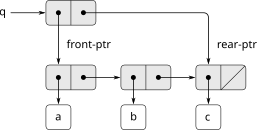
\includegraphics[width=69mm]{assets/figures/chapter_3/figure_3.19b.pdf}
\end{imageFigure}

To define the queue operations we use the following procedures, which enable us
to select and to modify the front and rear pointers of a queue:

\begin{codeBlock}
(define (front-ptr queue) (car queue))
(define (rear-ptr  queue) (cdr queue))
(define (set-front-ptr! queue item)
  (set-car! queue item))
(define (set-rear-ptr!  queue item)
  (set-cdr! queue item))
\end{codeBlock}

\noindent
Now we can implement the actual queue operations.  We will consider a queue to
be empty if its front pointer is the empty list:

\begin{codeBlock}
(define (empty-queue? queue)
  (null? (front-ptr queue)))
\end{codeBlock}

\noindent
The \code{make\-/queue} constructor returns, as an initially empty queue, a pair
whose \code{car} and \code{cdr} are both the empty list:

\begin{codeBlock}
(define (make-queue) (cons '() '()))
\end{codeBlock}

\noindent
To select the item at the front of the queue, we return the \code{car} of the
pair indicated by the front pointer:

\begin{codeBlock}
(define (front-queue queue)
  (if (empty-queue? queue)
      (error "FRONT called with an empty queue" queue)
      (car (front-ptr queue))))
\end{codeBlock}

% figure 3.20
\begin{imageFigure}
  {%
    Result of using \code{(insert\-/queue! q 'd)} on the queue of
    \link{Figure 3.19}.
  }%
  \includegraphics[width=88mm]{assets/figures/chapter_3/figure_3.20b.pdf}
\end{imageFigure}

\noindent
To insert an item in a queue, we follow the method whose result is indicated in
\link{Figure 3.20}.  We first create a new pair whose \code{car} is the item to
be inserted and whose \code{cdr} is the empty list.  If the queue was initially
empty, we set the front and rear pointers of the queue to this new pair.
Otherwise, we modify the final pair in the queue to point to the new pair, and
also set the rear pointer to the new pair.

\begin{codeBlock}
(define (insert-queue! queue item)
  (let ((new-pair (cons item '())))
    (cond ((empty-queue? queue)
           (set-front-ptr! queue new-pair)
           (set-rear-ptr! queue new-pair)
           queue)
          (else
           (set-cdr! (rear-ptr queue) new-pair)
           (set-rear-ptr! queue new-pair)
           queue))))
\end{codeBlock}

% figure 3.21
\begin{imageFigure}
  {%
    Result of using \code{(delete\-/queue!  q)} on the queue of
    \link{Figure 3.20}.
  }%
  \includegraphics[width=88mm]{assets/figures/chapter_3/figure_3.21b.pdf}
\end{imageFigure}

\noindent
To delete the item at the front of the queue, we merely modify the front
pointer so that it now points at the second item in the queue, which can be
found by following the \code{cdr} pointer of the first item (see
\link{Figure 3.21}):\footnote{If the first item is the final item in the queue, the front
pointer will be the empty list after the deletion, which will mark the queue as
empty; we needn't worry about updating the rear pointer, which will still point
to the deleted item, because \code{empty\-/queue?} looks only at the front
pointer.}

\begin{codeBlock}
(define (delete-queue! queue)
  (cond ((empty-queue? queue)
         (error
           "DELETE! called with an empty queue"
           queue))
        (else
          (set-front-ptr! queue
                          (cdr (front-ptr queue)))
          queue)))
\end{codeBlock}

\begin{exerciseGroup}
\phantomsection\label{Exercise 3.21}
\exerciseHeading{Exercise 3.21:} Ben Bitdiddle decides to test the
queue implementation described above.  He types in the procedures to the Lisp
interpreter and proceeds to try them out:

\begin{codeBlock}
(define q1 (make-queue))
(insert-queue! q1 'a)
~\textit{((a) a)}~
(insert-queue! q1 'b)
~\textit{((a b) b)}~
(delete-queue! q1)
~\textit{((b) b)}~
(delete-queue! q1)
~\textit{(() b)}~
\end{codeBlock}

``It's all wrong!'' he complains.  ``The interpreter's response shows that the
last item is inserted into the queue twice.  And when I delete both items, the
second \code{b} is still there, so the queue isn't empty, even though it's
supposed to be.''  Eva Lu Ator suggests that Ben has misunderstood what is
happening.  ``It's not that the items are going into the queue twice,'' she
explains.  ``It's just that the standard Lisp printer doesn't know how to make
sense of the queue representation.  If you want to see the queue printed
correctly, you'll have to define your own print procedure for queues.'' Explain
what Eva Lu is talking about.  In particular, show why Ben's examples produce
the printed results that they do.  Define a procedure \code{print\-/queue} that
takes a queue as input and prints the sequence of items in the queue.

\phantomsection\label{Exercise 3.22}
\exerciseHeading{Exercise 3.22:} Instead of representing a queue
as a pair of pointers, we can build a queue as a procedure with local state.
The local state will consist of pointers to the beginning and the end of an
ordinary list.  Thus, the \code{make\-/queue} procedure will have the form

\begin{codeBlock}
(define (make-queue)
  (let ((front-ptr ~\( \dots \)~ )
        (rear-ptr ~\( \dots \)~ ))
    ~\(\langle \)~~\var{definitions of internal procedures}~~\(\rangle \)~
    (define (dispatch m) ~\( \dots \)~)
    dispatch))
\end{codeBlock}

Complete the definition of \code{make\-/queue} and provide implementations of the
queue operations using this representation.

\phantomsection\label{Exercise 3.23}
\exerciseHeading{Exercise 3.23:} A \newterm{deque} (``double-ended
queue'') is a sequence in which items can be inserted and deleted at either the
front or the rear.  Operations on deques are the constructor \code{make\-/deque},
the predicate \code{empty\-/deque?}, selectors \code{front\-/deque} and
\code{rear\-/deque}, mutators \code{front\-/insert\-/deque!},
\code{rear\-/insert\-/deque!}, \code{front\-/delete\-/deque!}, and
\code{rear\-/delete\-/deque!}.  Show how to represent deques using pairs, and give
implementations of the operations.\footnote{Be careful not to make the
interpreter try to print a structure that contains cycles.  (See \link{Exercise 3.13}.)}
All operations should be accomplished in \( \Theta \)(1) steps.
\end{exerciseGroup}

\subsection{Representing Tables}
\label{Section 3.3.3}

When we studied various ways of representing sets in \link{Chapter 2}, we
mentioned in \link{Section 2.3.3} the task of maintaining a table of records
indexed by identifying keys.  In the implementation of data-directed
programming in \link{Section 2.4.3}, we made extensive use of two-dimensional
tables, in which information is stored and retrieved using two keys.  Here we
see how to build tables as mutable list structures.

% figure 3.22
\begin{imageFigure}
  {A table represented as a headed list.}
  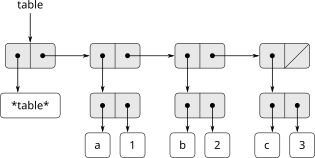
\includegraphics[width=81mm]{assets/figures/chapter_3/figure_3.22c.pdf}
\end{imageFigure}

We first consider a one-dimensional table, in which each value is stored under
a single key.  We implement the table as a list of records, each of which is
implemented as a pair consisting of a key and the associated value. The records
are glued together to form a list by pairs whose \code{car}s point to
successive records.  These gluing pairs are called the \newterm{backbone} of
the table.  In order to have a place that we can change when we add a new
record to the table, we build the table as a \newterm{headed list}.  A headed
list has a special backbone pair at the beginning, which holds a dummy
``record''---in this case the arbitrarily chosen symbol \code{*table*}.
\link{Figure 3.22} shows the box-and-pointer diagram for the table

\begin{codeBlock}
a:  1
b:  2
c:  3
\end{codeBlock}

\noindent
To extract information from a table we use the \code{lookup} procedure, which
takes a key as argument and returns the associated value (or false if there is
no value stored under that key).  \code{lookup} is defined in terms of the
\code{assoc} operation, which expects a key and a list of records as arguments.
Note that \code{assoc} never sees the dummy record.  \code{assoc} returns the
record that has the given key as its \code{car}.\footnote{Because \code{assoc}
uses \code{equal?}, it can recognize keys that are symbols, numbers, or list
structure.}  \code{lookup} then checks to see that the resulting record
returned by \code{assoc} is not false, and returns the value (the \code{cdr})
of the record.

\begin{codeBlock}
(define (lookup key table)
  (let ((record (assoc key (cdr table))))
    (if record
        (cdr record)
        false)))
(define (assoc key records)
  (cond ((null? records) false)
        ((equal? key (caar records)) (car records))
        (else (assoc key (cdr records)))))
\end{codeBlock}

\noindent
To insert a value in a table under a specified key, we first use \code{assoc}
to see if there is already a record in the table with this key.  If not, we
form a new record by \code{cons}ing the key with the value, and insert this at
the head of the table's list of records, after the dummy record.  If there
already is a record with this key, we set the \code{cdr} of this record to the
designated new value.  The header of the table provides us with a fixed
location to modify in order to insert the new record.\footnote{Thus, the first
backbone pair is the object that represents the table ``itself\( \kern0.1em \)''; that is, a
pointer to the table is a pointer to this pair.  This same backbone pair always
starts the table.  If we did not arrange things in this way, \code{insert!}
would have to return a new value for the start of the table when it added a new
record.}

\begin{codeBlock}
(define (insert! key value table)
  (let ((record (assoc key (cdr table))))
    (if record
        (set-cdr! record value)
        (set-cdr! table
                  (cons (cons key value)
                        (cdr table)))))
  'ok)
\end{codeBlock}

\noindent
To construct a new table, we simply create a list containing the symbol
\code{*table*}:

\begin{codeBlock}
(define (make-table)
  (list '*table*))
\end{codeBlock}

\subsubsection*{Two-dimensional tables}

\noindent
In a two-dimensional table, each value is indexed by two keys.  We can
construct such a table as a one-dimensional table in which each key identifies
a subtable.  \link{Figure 3.23} shows the box-and-pointer diagram for the table

\begin{example}
math:    +:  43        letters:    a:  97
         -:  45                    b:  98
         *:  42
\end{example}

\noindent
which has two subtables.  (The subtables don't need a special header symbol,
since the key that identifies the subtable serves this purpose.)

When we look up an item, we use the first key to identify the correct subtable.
Then we use the second key to identify the record within the subtable.

\begin{codeBlock}
(define (lookup key-1 key-2 table)
  (let ((subtable
         (assoc key-1 (cdr table))))
    (if subtable
        (let ((record
               (assoc key-2 (cdr subtable))))
          (if record
              (cdr record)
              false))
        false)))
\end{codeBlock}

% figure 3.23
\begin{imageFigure}
  {A two-dimensional table.}
  \includegraphics[width=103mm]{assets/figures/chapter_3/figure_3.23a.pdf}
\end{imageFigure}

To insert a new item under a pair of keys, we use \code{assoc} to see if there
is a subtable stored under the first key.  If not, we build a new subtable
containing the single record (\code{key\-/2}, \code{value}) and insert it into
the table under the first key.  If a subtable already exists for the first key,
we insert the new record into this subtable, using the insertion method for
one-dimensional tables described above:

\begin{codeBlock}
(define (insert! key-1 key-2 value table)
  (let ((subtable (assoc key-1 (cdr table))))
    (if subtable
        (let ((record (assoc key-2 (cdr subtable))))
          (if record
              (set-cdr! record value)
              (set-cdr! subtable
                        (cons (cons key-2 value)
                              (cdr subtable)))))
        (set-cdr! table
                  (cons (list key-1
                              (cons key-2 value))
                        (cdr table)))))
  'ok)
\end{codeBlock}

\subsubsection*{Creating local tables}

The \code{lookup} and \code{insert!} operations defined above take the table as
an argument.  This enables us to use programs that access more than one table.
Another way to deal with multiple tables is to have separate \code{lookup} and
\code{insert!} procedures for each table.  We can do this by representing a
table procedurally, as an object that maintains an internal table as part of
its local state.  When sent an appropriate message, this ``table object''
supplies the procedure with which to operate on the internal table.  Here is a
generator for two-dimensional tables represented in this fashion:

\begin{codeBlock}
(define (make-table)
  (let ((local-table (list '*table*)))
    (define (lookup key-1 key-2)
      (let ((subtable
              (assoc key-1 (cdr local-table))))
        (if subtable
            (let ((record
                    (assoc key-2 (cdr subtable))))
              (if record (cdr record) false))
            false)))
    (define (insert! key-1 key-2 value)
      (let ((subtable
              (assoc key-1 (cdr local-table))))
        (if subtable
            (let ((record
                    (assoc key-2 (cdr subtable))))
              (if record
                  (set-cdr! record value)
                  (set-cdr! subtable
                            (cons (cons key-2 value)
                                  (cdr subtable)))))
            (set-cdr! local-table
                      (cons (list key-1
                                  (cons key-2 value))
                            (cdr local-table)))))
      'ok)
    (define (dispatch m)
      (cond ((eq? m 'lookup-proc) lookup)
            ((eq? m 'insert-proc!) insert!)
            (else
              (error "Unknown operation: TABLE"
                     m))))
    dispatch))
\end{codeBlock}

\noindent
Using \code{make\-/table}, we could implement the \code{get} and \code{put}
operations used in \link{Section 2.4.3} for data-directed programming, as
follows:

\begin{codeBlock}
(define operation-table (make-table))
(define get (operation-table 'lookup-proc))
(define put (operation-table 'insert-proc!))
\end{codeBlock}

\noindent
\code{get} takes as arguments two keys, and \code{put} takes as arguments two
keys and a value.  Both operations access the same local table, which is
encapsulated within the object created by the call to \code{make\-/table}.

\begin{exerciseGroup}
\phantomsection\label{Exercise 3.24}
\exerciseHeading{Exercise 3.24:} In the table implementations
above, the keys are tested for equality using \code{equal?} (called by
\code{assoc}).  This is not always the appropriate test.  For instance, we
might have a table with numeric keys in which we don't need an exact match to
the number we're looking up, but only a number within some tolerance of it.
Design a table constructor \code{make\-/table} that takes as an argument a
\code{same\-/key?} procedure that will be used to test ``equality'' of keys.
\code{make\-/table} should return a \code{dispatch} procedure that can be used to
access appropriate \code{lookup} and \code{insert!} procedures for a local
table.

\phantomsection\label{Exercise 3.25}
\exerciseHeading{Exercise 3.25:} Generalizing one- and
two-dimensional tables, show how to implement a table in which values are
stored under an arbitrary number of keys and different values may be stored
under different numbers of keys.  The \code{lookup} and \code{insert!}
procedures should take as input a list of keys used to access the table.

\phantomsection\label{Exercise 3.26}
\exerciseHeading{Exercise 3.26:} To search a table as implemented
above, one needs to scan through the list of records.  This is basically the
unordered list representation of \link{Section 2.3.3}.  For large tables, it may
be more efficient to structure the table in a different manner.  Describe a
table implementation where the (key, value) records are organized using a
binary tree, assuming that keys can be ordered in some way (e.g., numerically
or alphabetically).  (Compare \link{Exercise 2.66} of \link{Chapter 2}.)

\phantomsection\label{Exercise 3.27}
\exerciseHeading{Exercise 3.27:} \newterm{Memoization} (also
called \newterm{tabulation}) is a technique that enables a procedure to record,
in a local table, values that have previously been computed.  This technique
can make a vast difference in the performance of a program.  A memoized
procedure maintains a table in which values of previous calls are stored using
as keys the arguments that produced the values.  When the memoized procedure is
asked to compute a value, it first checks the table to see if the value is
already there and, if so, just returns that value.  Otherwise, it computes the
new value in the ordinary way and stores this in the table.  As an example of
memoization, recall from \link{Section 1.2.2} the exponential process for
computing Fibonacci numbers:

\begin{codeBlock}
(define (fib n)
  (cond ((= n 0) 0)
        ((= n 1) 1)
        (else (+ (fib (- n 1)) (fib (- n 2))))))
\end{codeBlock}

The memoized version of the same procedure is

\begin{codeBlock}
(define memo-fib
  (memoize
   (lambda (n)
     (cond ((= n 0) 0)
           ((= n 1) 1)
           (else (+ (memo-fib (- n 1))
                    (memo-fib (- n 2))))))))
\end{codeBlock}

\noindent
where the memoizer is defined as

\begin{codeBlock}
(define (memoize f)
  (let ((table (make-table)))
    (lambda (x)
      (let ((previously-computed-result
             (lookup x table)))
        (or previously-computed-result
            (let ((result (f x)))
              (insert! x result table)
              result))))))
\end{codeBlock}

Draw an environment diagram to analyze the computation of \code{(memo\-/fib 3)}.
Explain why \code{memo\-/fib} computes the \( n^{\mathrm{th}} \) Fibonacci number in a number
of steps proportional to \( n \).  Would the scheme still work if we had simply
defined \code{memo\-/fib} to be \code{(memoize fib)}?
\end{exerciseGroup}

\subsection{A Simulator for Digital Circuits}
\label{Section 3.3.4}

Designing complex digital systems, such as computers, is an important
engineering activity.  Digital systems are constructed by interconnecting
simple elements.  Although the behavior of these individual elements is simple,
networks of them can have very complex behavior.  Computer simulation of
proposed circuit designs is an important tool used by digital systems
engineers.  In this section we design a system for performing digital logic
simulations.  This system typifies a kind of program called an
\newterm{event-driven simulation}, in which actions (``events'') trigger
further events that happen at a later time, which in turn trigger more events,
and so on.

Our computational model of a circuit will be composed of objects that
correspond to the elementary components from which the circuit is constructed.
There are \newterm{wires}, which carry \newterm{digital signals}.  A digital
signal may at any moment have only one of two possible values, 0 and 1.  There
are also various types of digital \newterm{function boxes}, which connect wires
carrying input signals to other output wires.  Such boxes produce output
signals computed from their input signals.  The output signal is delayed by a
time that depends on the type of the function box.  For example, an
\newterm{inverter} is a primitive function box that inverts its input.  If the
input signal to an inverter changes to 0, then one inverter-delay later the
inverter will change its output signal to 1.  If the input signal to an
inverter changes to 1, then one inverter-delay later the inverter will change
its output signal to 0.  We draw an inverter symbolically as in \link{Figure 3.24}.
An \newterm{and-gate}, also shown in \link{Figure 3.24}, is a primitive
function box with two inputs and one output.  It drives its output signal to a
value that is the \newterm{logical and} of the inputs.  That is, if both of its
input signals become 1, then one and-gate-delay time later the and-gate will
force its output signal to be 1; otherwise the output will be 0.  An
\newterm{or-gate} is a similar two-input primitive function box that drives its
output signal to a value that is the \newterm{logical or} of the inputs.  That
is, the output will become 1 if at least one of the input signals is 1;
otherwise the output will become 0.

% figure 3.24
\begin{imageFigure}
  {Primitive functions in the digital logic simulator.}
  
\includegraphics[width=74mm]{assets/figures/chapter_3/figure_3.24b.pdf}
\end{imageFigure}

We can connect primitive functions together to construct more complex
functions.  To accomplish this we wire the outputs of some function boxes to
the inputs of other function boxes.  For example, the \newterm{half-adder}
circuit shown in \link{Figure 3.25} consists of an or-gate, two and-gates, and
an inverter.  It takes two input signals, A and B, and has two output signals,
S and C.  S will become 1 whenever precisely one of A and B is 1, and C will
become 1 whenever A and B are both 1.  We can see from the figure that, because
of the delays involved, the outputs may be generated at different times.  Many
of the difficulties in the design of digital circuits arise from this fact.

% figure 3.25
\begin{imageFigure}
  {A half-adder circuit.}
  \includegraphics[width=72mm]{assets/figures/chapter_3/figure_3.25c.pdf}
\end{imageFigure}

We will now build a program for modeling the digital logic circuits we wish to
study.  The program will construct computational objects modeling the wires,
which will ``hold'' the signals.  Function boxes will be modeled by procedures
that enforce the correct relationships among the signals.

One basic element of our simulation will be a procedure \code{make\-/wire}, which
constructs wires.  For example, we can construct six wires as follows:

\begin{codeBlock}
(define a (make-wire))
(define b (make-wire))
(define c (make-wire))
(define d (make-wire))
(define e (make-wire))
(define s (make-wire))
\end{codeBlock}

\noindent
We attach a function box to a set of wires by calling a procedure that
constructs that kind of box.  The arguments to the constructor procedure are
the wires to be attached to the box.  For example, given that we can construct
and-gates, or-gates, and inverters, we can wire together the half-adder shown
in \link{Figure 3.25}:

\begin{codeBlock}
(or-gate a b d)
~\textit{ok}~
(and-gate a b c)
~\textit{ok}~
(inverter c e)
~\textit{ok}~
(and-gate d e s)
~\textit{ok}~
\end{codeBlock}

\noindent
Better yet, we can explicitly name this operation by defining a procedure
\code{half\-/adder} that constructs this circuit, given the four external wires
to be attached to the half-adder:

\begin{codeBlock}
(define (half-adder a b s c)
  (let ((d (make-wire)) (e (make-wire)))
    (or-gate a b d)
    (and-gate a b c)
    (inverter c e)
    (and-gate d e s)
    'ok))
\end{codeBlock}

\noindent
The advantage of making this definition is that we can use \code{half\-/adder}
itself as a building block in creating more complex circuits.  \link{Figure 3.26},
for example, shows a \newterm{full-adder} composed of two half-adders
and an or-gate.\footnote{A full-adder is a basic circuit element used in adding
two binary numbers.  Here A and B are the bits at corresponding positions in
the two numbers to be added, and \( \rm C_{in} \) is the carry bit from the
addition one place to the right.  The circuit generates SUM, which is the sum
bit in the corresponding position, and \( \rm C_{out} \), which is the carry
bit to be propagated to the left.} We can construct a full-adder as follows:

\begin{codeBlock}
(define (full-adder a b c-in sum c-out)
  (let ((s (make-wire)) (c1 (make-wire))
                        (c2 (make-wire)))
    (half-adder b c-in s c1)
    (half-adder a s sum c2)
    (or-gate c1 c2 c-out)
    'ok))
\end{codeBlock}

% figure 3.26
\begin{imageFigure}
  {A full-adder circuit.}
  \includegraphics[width=74mm]{assets/figures/chapter_3/figure_3.26a.pdf}
\end{imageFigure}

\noindent
Having defined \code{full\-/adder} as a procedure, we can now use it as a
building block for creating still more complex circuits.  (For example, see
\link{Exercise 3.30}.)

In essence, our simulator provides us with the tools to construct a language of
circuits.  If we adopt the general perspective on languages with which we
approached the study of Lisp in \link{Section 1.1}, we can say that the
primitive function boxes form the primitive elements of the language, that
wiring boxes together provides a means of combination, and that specifying
wiring patterns as procedures serves as a means of abstraction.

\subsubsection*{Primitive function boxes}

The primitive function boxes implement the ``forces'' by which a change in the
signal on one wire influences the signals on other wires.  To build function
boxes, we use the following operations on wires:

\begin{itemize}
\item \texttt{(get-signal} $\langle\texttt{\textsl{wire}}\rangle$\texttt{)}

\noindent
returns the current value of the signal on the wire.

\item \code{(set-signal!} $\langle\texttt{\textsl{wire}}\rangle$ $\langle\texttt{\textsl{new value}}\rangle$\texttt{)}

\noindent
changes the value of the signal on the wire to the new value.

\item \code{(add-action!} $\langle\texttt{\textsl{wire}}\rangle$ $\langle\texttt{\textsl{procedure of no arguments}}\rangle$\texttt{)}

\noindent
asserts that the designated procedure should be run whenever the signal on the
wire changes value.  Such procedures are the vehicles by which changes in the
signal value on the wire are communicated to other wires.
\end{itemize}

\noindent
In addition, we will make use of a procedure \code{after\-/delay} that takes a
time delay and a procedure to be run and executes the given procedure after the
given delay.

Using these procedures, we can define the primitive digital logic functions.
To connect an input to an output through an inverter, we use \code{add\-/action!}
to associate with the input wire a procedure that will be run whenever the
signal on the input wire changes value.  The procedure computes the
\code{logical\-/not} of the input signal, and then, after one
\code{inverter\-/delay}, sets the output signal to be this new value:

\begin{codeBlock}
(define (inverter input output)
  (define (invert-input)
    (let ((new-value (logical-not (get-signal input))))
      (after-delay
       inverter-delay
       (lambda () (set-signal! output new-value)))))
  (add-action! input invert-input) 'ok)
(define (logical-not s)
  (cond ((= s 0) 1)
        ((= s 1) 0)
        (else (error "Invalid signal" s))))
\end{codeBlock}

\noindent
An and-gate is a little more complex.  The action procedure must be run if
either of the inputs to the gate changes.  It computes the \code{logical\-/and}
(using a procedure analogous to \code{logical\-/not}) of the values of the
signals on the input wires and sets up a change to the new value to occur on
the output wire after one \code{and\-/gate\-/delay}.

\begin{codeBlock}
(define (and-gate a1 a2 output)
  (define (and-action-procedure)
    (let
      ((new-value (logical-and
                      (get-signal a1)
                      (get-signal a2))))
      (after-delay
       and-gate-delay
       (lambda () (set-signal! output new-value)))))
  (add-action! a1 and-action-procedure)
  (add-action! a2 and-action-procedure)
  'ok)
\end{codeBlock}

\begin{exerciseGroup}
\phantomsection\label{Exercise 3.28}
\exerciseHeading{Exercise 3.28:} Define an or-gate as a primitive
function box.  Your \code{or\-/gate} constructor should be similar to
\code{and\-/gate}.

\phantomsection\label{Exercise 3.29}
\exerciseHeading{Exercise 3.29:} Another way to construct an
or-gate is as a compound digital logic device, built from and-gates and
inverters.  Define a procedure \code{or\-/gate} that accomplishes this.  What is
the delay time of the or-gate in terms of \code{and\-/gate\-/delay} and
\code{inverter\-/delay}?

\phantomsection\label{Exercise 3.30}
\exerciseHeading{Exercise 3.30:} \link{Figure 3.27} shows a
\newterm{ripple-carry adder} formed by stringing together \( n \) full-adders.
This is the simplest form of parallel adder for adding two \( n \)-bit binary
numbers.  The inputs \( A_1 \), \( A_2 \), \( A_3 \), \( \dots \), \( A_n \) and
\( B_1 \), \( B_2 \), \( B_3 \),
\( \dots \), \( B_n \) are the two binary numbers to be added (each \( A_k \) and
\( B_k \) is a 0 or a 1).  The circuit generates \( S_1 \), \( S_2 \),
\( S_3 \), \( \dots \), \( S_n \),
the \( n \) bits of the sum, and \( C \), the carry from the addition.  Write a
procedure \code{ripple\-/carry\-/adder} that generates this circuit.  The procedure
should take as arguments three lists of \( n \) wires each---the \( A_k \), the
\( B_k \), and the \( S_k \)---and also another wire \( C \).  The major drawback of the
ripple-carry adder is the need to wait for the carry signals to propagate.
What is the delay needed to obtain the complete output from an \( n \)-bit
ripple-carry adder, expressed in terms of the delays for and-gates, or-gates,
and inverters?

% figure 3.27
\begin{imageFigure}
  {A ripple-carry adder for \( n \)-bit numbers.}
  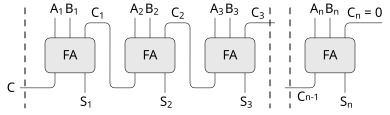
\includegraphics[width=96mm]{assets/figures/chapter_3/figure_3.27a.pdf}
\end{imageFigure}

\end{exerciseGroup}

\subsubsection*{Representing wires}

A wire in our simulation will be a computational object with two local state
variables: a \code{signal\-/value} (initially taken to be 0) and a collection of
\code{action\-/procedures} to be run when the signal changes value.  We implement
the wire, using message-passing style, as a collection of local procedures
together with a \code{dispatch} procedure that selects the appropriate local
operation, just as we did with the simple bank-account object in
\link{Section 3.1.1}:

\begin{codeBlock}
(define (make-wire)
  (let ((signal-value 0) (action-procedures '()))
    (define (set-my-signal! new-value)
      (if (not (= signal-value new-value))
          (begin (set! signal-value new-value)
            (call-each action-procedures))
          'done))
    (define (accept-action-procedure! proc)
      (set! action-procedures
            (cons proc action-procedures))
      (proc))
    (define (dispatch m)
      (cond ((eq? m 'get-signal) signal-value)
            ((eq? m 'set-signal!) set-my-signal!)
            ((eq? m 'add-action!)
             accept-action-procedure!)
            (else
              (error "Unknown operation: WIRE"
                     m))))
    dispatch))
\end{codeBlock}

\noindent
The local procedure \code{set\-/my\-/signal!} tests whether the new signal value
changes the signal on the wire.  If so, it runs each of the action procedures,
using the following procedure \code{call\-/each}, which calls each of the items
in a list of no-argument procedures:

\begin{codeBlock}
(define (call-each procedures)
  (if (null? procedures)
      'done
      (begin ((car procedures))
             (call-each (cdr procedures)))))
\end{codeBlock}

\noindent
The local procedure \code{accept\-/action\-/procedure!} adds the given procedure to
the list of procedures to be run, and then runs the new procedure once.  (See
\link{Exercise 3.31}.)

With the local \code{dispatch} procedure set up as specified, we can provide
the following procedures to access the local operations on
wires:\footnote{\label{Footnote 27} These procedures are simply
syntactic sugar that allow us to use ordinary procedural syntax to access the
local procedures of objects.  It is striking that we can interchange the role
of ``procedures'' and ``data'' in such a simple way.  For example, if we write
\code{(wire 'get\-/signal)} we think of \code{wire} as a procedure that is called
with the message \code{get\-/signal} as input.  Alternatively, writing
\code{(get\-/signal wire)} encourages us to think of \code{wire} as a data object
that is the input to a procedure \code{get\-/signal}.  The truth of the matter is
that, in a language in which we can deal with procedures as objects, there is
no fundamental difference between ``procedures'' and ``data,'' and we can
choose our syntactic sugar to allow us to program in whatever style we choose.}

\begin{codeBlock}
(define (get-signal wire) (wire 'get-signal))
(define (set-signal! wire new-value)
  ((wire 'set-signal!) new-value))
(define (add-action! wire action-procedure)
  ((wire 'add-action!) action-procedure))
\end{codeBlock}

\noindent
Wires, which have time-varying signals and may be incrementally attached to
devices, are typical of mutable objects.  We have modeled them as procedures
with local state variables that are modified by assignment.  When a new wire is
created, a new set of state variables is allocated (by the \code{let}
expression in \code{make\-/wire}) and a new \code{dispatch} procedure is
constructed and returned, capturing the environment with the new state
variables.

The wires are shared among the various devices that have been connected to
them.  Thus, a change made by an interaction with one device will affect all
the other devices attached to the wire.  The wire communicates the change to
its neighbors by calling the action procedures provided to it when the
connections were established.

\subsubsection*{The agenda}

The only thing needed to complete the simulator is \code{after\-/delay}.  The
idea here is that we maintain a data structure, called an \newterm{agenda},
that contains a schedule of things to do.  The following operations are defined
for agendas:

\begin{itemize}
\item
\code{(make-agenda)} returns a new empty agenda.

\item
\code{(empty-agenda?} $\langle\texttt{\textsl{agenda}}\rangle$\texttt{)} is true if the specified agenda is
empty.
\item
\code{(first-agenda-item} $\langle\texttt{\textsl{agenda}}\rangle$\texttt{)} returns the first item on the
agenda.
\item
\code{(remove-first-agenda-item!} $\langle\texttt{\textsl{agenda}}\rangle$\texttt{)} modifies the agenda by
removing the first item.
\item
\code{(add-to-agenda!} $\langle\texttt{\textsl{time}}\rangle$ $\langle\texttt{\textsl{action}}\rangle$ $\langle\texttt{\textsl{agenda}}\rangle$\texttt{)} modifies the agenda by adding the given action procedure to be run at the specified time.
\item
\code{(current-time} $\langle\texttt{\textsl{agenda}}\rangle$\texttt{)} returns the current simulation time.
\end{itemize}

\noindent
The particular agenda that we use is denoted by \code{the\-/agenda}.  The
procedure \code{after\-/delay} adds new elements to \code{the\-/agenda}:

\begin{codeBlock}
(define (after-delay delay action)
  (add-to-agenda! (+ delay (current-time the-agenda))
                  action
                  the-agenda))
\end{codeBlock}

\noindent
The simulation is driven by the procedure \code{propagate}, which operates on
\code{the\-/agenda}, executing each procedure on the agenda in sequence.  In
general, as the simulation runs, new items will be added to the agenda, and
\code{propagate} will continue the simulation as long as there are items on the
agenda:

\begin{codeBlock}
(define (propagate)
  (if (empty-agenda? the-agenda)
      'done
      (let ((first-item
              (first-agenda-item the-agenda)))
        (first-item)
        (remove-first-agenda-item! the-agenda)
        (propagate))))
\end{codeBlock}

\subsubsection*{A sample simulation}

The following procedure, which places a ``probe'' on a wire, shows the
simulator in action.  The probe tells the wire that, whenever its signal
changes value, it should print the new signal value, together with the current
time and a name that identifies the wire:

\begin{codeBlock}
(define (probe name wire)
  (add-action! wire
               (lambda ()
                 (newline)
                 (display name) (display " ")
                 (display (current-time the-agenda))
                 (display "  New-value = ")
                 (display (get-signal wire)))))
\end{codeBlock}

\noindent
We begin by initializing the agenda and specifying delays for the primitive
function boxes:

\begin{codeBlock}
(define the-agenda (make-agenda))
(define inverter-delay 2)
(define and-gate-delay 3)
(define or-gate-delay 5)
\end{codeBlock}

\noindent
Now we define four wires, placing probes on two of them:

\begin{codeBlock}
(define input-1 (make-wire))
(define input-2 (make-wire))
(define sum (make-wire))
(define carry (make-wire))

(probe 'sum sum)
~\textit{sum 0  New-value = 0}~

(probe 'carry carry)
~\textit{carry 0  New-value = 0}~
\end{codeBlock}

\noindent
Next we connect the wires in a half-adder circuit (as in \link{Figure 3.25}),
set the signal on \code{input\-/1} to 1, and run the simulation:

\begin{codeBlock}
(half-adder input-1 input-2 sum carry)
~\textit{ok}~
\end{codeBlock}

\begin{codeBlock}
(set-signal! input-1 1)
~\textit{done}~
\end{codeBlock}

\begin{codeBlock}
(propagate)
~\textit{sum 8  New-value = 1}~
~\textit{done}~
\end{codeBlock}

\noindent
The \code{sum} signal changes to 1 at time 8.  We are now eight time units from
the beginning of the simulation.  At this point, we can set the signal on
\code{input\-/2} to 1 and allow the values to propagate:

\begin{codeBlock}
(set-signal! input-2 1)
~\textit{done}~
\end{codeBlock}

\begin{codeBlock}
(propagate)
~\textit{carry 11  New-value = 1}~
~\textit{sum 16  New-value = 0}~
~\textit{done}~
\end{codeBlock}

\noindent
The \code{carry} changes to 1 at time 11 and the \code{sum} changes to 0 at
time 16.

\begin{exerciseGroup}
\phantomsection\label{Exercise 3.31}
\exerciseHeading{Exercise 3.31:} The internal procedure
\code{accept\-/action\-/procedure!} defined in \code{make\-/wire} specifies that when
a new action procedure is added to a wire, the procedure is immediately run.
Explain why this initialization is necessary.  In particular, trace through the
half-adder example in the paragraphs above and say how the system's response
would differ if we had defined \code{accept\-/action\-/procedure!} as

\begin{codeBlock}
(define (accept-action-procedure! proc)
  (set! action-procedures
        (cons proc action-procedures)))
\end{codeBlock}
\end{exerciseGroup}

\subsubsection*{Implementing the agenda}

Finally, we give details of the agenda data structure, which holds the
procedures that are scheduled for future execution.

The agenda is made up of \newterm{time segments}.  Each time segment is a pair
consisting of a number (the time) and a queue (see \link{Exercise 3.32}) that
holds the procedures that are scheduled to be run during that time segment.

\begin{codeBlock}
(define (make-time-segment time queue)
  (cons time queue))
(define (segment-time s) (car s))
(define (segment-queue s) (cdr s))
\end{codeBlock}

\noindent
We will operate on the time-segment queues using the queue operations described
in \link{Section 3.3.2}.

The agenda itself is a one-dimensional table of time segments.  It differs from
the tables described in \link{Section 3.3.3} in that the segments will be sorted
in order of increasing time.  In addition, we store the \newterm{current time}
(i.e., the time of the last action that was processed) at the head of the
agenda.  A newly constructed agenda has no time segments and has a current time
of 0:\footnote{The agenda is a headed list, like the tables in
\link{Section 3.3.3}, but since the list is headed by the time, we do not need an
additional dummy header (such as the \code{*table*} symbol used with tables).}

\begin{codeBlock}
(define (make-agenda) (list 0))
(define (current-time agenda) (car agenda))
(define (set-current-time! agenda time)
  (set-car! agenda time))
(define (segments agenda) (cdr agenda))
(define (set-segments! agenda segments)
  (set-cdr! agenda segments))
(define (first-segment agenda) (car (segments agenda)))
(define (rest-segments agenda) (cdr (segments agenda)))
\end{codeBlock}

\noindent
An agenda is empty if it has no time segments:

\begin{codeBlock}
(define (empty-agenda? agenda)
  (null? (segments agenda)))
\end{codeBlock}

\noindent
To add an action to an agenda, we first check if the agenda is empty.  If so,
we create a time segment for the action and install this in the agenda.
Otherwise, we scan the agenda, examining the time of each segment.  If we find
a segment for our appointed time, we add the action to the associated queue.
If we reach a time later than the one to which we are appointed, we insert a
new time segment into the agenda just before it.  If we reach the end of the
agenda, we must create a new time segment at the end.

\begin{codeBlock}
(define (add-to-agenda! time action agenda)
  (define (belongs-before? segments)
    (or (null? segments)
        (< time (segment-time (car segments)))))
  (define (make-new-time-segment time action)
    (let ((q (make-queue)))
      (insert-queue! q action)
      (make-time-segment time q)))
  (define (add-to-segments! segments)
    (if (= (segment-time (car segments)) time)
        (insert-queue! (segment-queue (car segments))
                       action)
        (let ((rest (cdr segments)))
          (if (belongs-before? rest)
              (set-cdr!
                segments
                (cons (make-new-time-segment time
                                             action)
                      (cdr segments)))
              (add-to-segments! rest)))))
  (let ((segments (segments agenda)))
    (if (belongs-before? segments)
        (set-segments!
          agenda
          (cons (make-new-time-segment time action)
                segments))
        (add-to-segments! segments))))
\end{codeBlock}

\noindent
The procedure that removes the first item from the agenda deletes the item at
the front of the queue in the first time segment.  If this deletion makes the
time segment empty, we remove it from the list of segments:\footnote{Observe
that the \code{if} expression in this procedure has no \( \langle \)\var{alternative}\( \kern0.08em\rangle \)
expression.  Such a ``one-armed \code{if} statement'' is used to decide whether
to do something, rather than to select between two expressions.  An \code{if}
expression returns an unspecified value if the predicate is false and there is
no \( \langle \)\var{alternative}\( \kern0.08em\rangle \).}

\begin{codeBlock}
(define (remove-first-agenda-item! agenda)
  (let ((q (segment-queue (first-segment agenda))))
    (delete-queue! q)
    (if (empty-queue? q)
        (set-segments! agenda (rest-segments agenda)))))
\end{codeBlock}

\noindent
The first agenda item is found at the head of the queue in the first time
segment.  Whenever we extract an item, we also update the current
time:\footnote{In this way, the current time will always be the time of the
action most recently processed.  Storing this time at the head of the agenda
ensures that it will still be available even if the associated time segment has
been deleted.}

\begin{codeBlock}
(define (first-agenda-item agenda)
  (if (empty-agenda? agenda)
      (error "Agenda is empty: FIRST-AGENDA-ITEM")
      (let ((first-seg (first-segment agenda)))
        (set-current-time! agenda
                           (segment-time first-seg))
        (front-queue (segment-queue first-seg)))))
\end{codeBlock}

\begin{exerciseGroup}
\phantomsection\label{Exercise 3.32}
\exerciseHeading{Exercise 3.32:} The procedures to be run during
each time segment of the agenda are kept in a queue.  Thus, the procedures for
each segment are called in the order in which they were added to the agenda
(first in, first out).  Explain why this order must be used.  In particular,
trace the behavior of an and-gate whose inputs change from 0, 1 to 1, 0 in the
same segment and say how the behavior would differ if we stored a segment's
procedures in an ordinary list, adding and removing procedures only at the
front (last in, first out).
\end{exerciseGroup}


\subsection{Propagation of Constraints}
\label{Section 3.3.5}

Computer programs are traditionally organized as one-directional computations,
which perform operations on prespecified arguments to produce desired outputs.
On the other hand, we often model systems in terms of relations among
quantities.  For example, a mathematical model of a mechanical structure might
include the information that the deflection \( d \) of a metal rod is related to
the force \( F \) on the rod, the length \( L \) of the rod, the cross-sectional
area \( A \), and the elastic modulus \( E \) via the equation

$$ dAE = FL. $$

Such an equation is not one-directional.  Given any four of the quantities, we
can use it to compute the fifth.  Yet translating the equation into a
traditional computer language would force us to choose one of the quantities to
be computed in terms of the other four.  Thus, a procedure for computing the
area \( A \) could not be used to compute the deflection \( d \), even though the
computations of \( A \) and \( d \) arise from the same
equation.\footnote{Constraint propagation first appeared in the incredibly
forward-looking \acronym{SKETCHPAD} system of Ivan \link{Sutherland (1963)}.  A
beautiful constraint-propagation system based on the Smalltalk language was
developed by Alan \link{Borning (1977)} at Xerox Palo Alto Research Center.  Sussman,
Stallman, and Steele applied constraint propagation to electrical circuit
analysis (\link{Sussman and Stallman 1975}; \link{Sussman and Steele 1980}). TK!Solver
(\link{Konopasek and Jayaraman 1984}) is an extensive modeling environment based on
constraints.}

In this section, we sketch the design of a language that enables us to work in
terms of relations themselves.  The primitive elements of the language are
\newterm{primitive constraints}, which state that certain relations hold
between quantities.  For example, \code{(adder a b c)} specifies that the
quantities \( a \), \( b \), and \( c \) must be related by the equation
\( a + b = c \), \code{(multiplier x y z)} expresses the constraint
\( xy = z \), and \code{(constant 3.14 x)} says that the value of \( x \) must be 3.14.

Our language provides a means of combining primitive constraints in order to
express more complex relations.  We combine constraints by constructing
\newterm{constraint networks}, in which constraints are joined by
\newterm{connectors}.  A connector is an object that ``holds'' a value that may
participate in one or more constraints.  For example, we know that the
relationship between Fahrenheit and Celsius temperatures is

$$ 9C = 5(F - 32). $$

Such a constraint can be thought of as a network consisting of primitive adder,
multiplier, and constant constraints (\link{Figure 3.28}).  In the figure, we
see on the left a multiplier box with three terminals, labeled \( {m1} \), \( {m2} \),
and \( p \).  These connect the multiplier to the rest of the network as follows:
The \( {m1} \) terminal is linked to a connector \( C \), which will hold the Celsius
temperature.  The \( {m2} \) terminal is linked to a connector \( w \), which is also
linked to a constant box that holds 9.  The \( p \) terminal, which the
multiplier box constrains to be the product of \( {m1} \) and \( {m2} \), is linked to
the \( p \) terminal of another multiplier box, whose \( {m2} \) is connected to a
constant 5 and whose \( {m1} \) is connected to one of the terms in a sum.

% figure 3.28
\begin{imageFigure}
  {The relation \( 9C = 5(F - 32) \) expressed as a constraint network.}
  \includegraphics[width=87mm]{assets/figures/chapter_3/figure_3.28.pdf}
\end{imageFigure}

Computation by such a network proceeds as follows: When a connector is given a
value (by the user or by a constraint box to which it is linked), it awakens
all of its associated constraints (except for the constraint that just awakened
it) to inform them that it has a value.  Each awakened constraint box then
polls its connectors to see if there is enough information to determine a value
for a connector.  If so, the box sets that connector, which then awakens all of
its associated constraints, and so on.  For instance, in conversion between
Celsius and Fahrenheit, \( w \), \( x \), and \( y \) are immediately set by the
constant boxes to 9, 5, and 32, respectively.  The connectors awaken the
multipliers and the adder, which determine that there is not enough information
to proceed.  If the user (or some other part of the network) sets \( C \) to a
value (say 25), the leftmost multiplier will be awakened, and it will set \( u \)
to \( 25 \cdot 9 = 225 \).  Then \( u \) awakens the second multiplier, which sets \( v \) to
45, and \( v \) awakens the adder, which sets \( F \) to 77.

\subsubsection*{Using the constraint system}

To use the constraint system to carry out the temperature computation outlined
above, we first create two connectors, \code{C} and \code{F}, by calling the
constructor \code{make\-/connector}, and link \code{C} and \code{F} in an
appropriate network:

\begin{codeBlock}
(define C (make-connector))
(define F (make-connector))
(celsius-fahrenheit-converter C F)
~\textit{ok}~
\end{codeBlock}

\noindent
The procedure that creates the network is defined as follows:

\begin{codeBlock}
(define (celsius-fahrenheit-converter c f)
  (let ((u (make-connector))
        (v (make-connector))
        (w (make-connector))
        (x (make-connector))
        (y (make-connector)))
    (multiplier c w u)
    (multiplier v x u)
    (adder v y f)
    (constant 9 w)
    (constant 5 x)
    (constant 32 y)
    'ok))
\end{codeBlock}

\noindent
This procedure creates the internal connectors \code{u}, \code{v}, \code{w},
\code{x}, and \code{y}, and links them as shown in \link{Figure 3.28} using the
primitive constraint constructors \code{adder}, \code{multiplier}, and
\code{constant}.  Just as with the digital-circuit simulator of
\link{Section 3.3.4}, expressing these combinations of primitive elements in terms of
procedures automatically provides our language with a means of abstraction for
compound objects.

To watch the network in action, we can place probes on the connectors \code{C}
and \code{F}, using a \code{probe} procedure similar to the one we used to
monitor wires in \link{Section 3.3.4}.  Placing a probe on a connector will
cause a message to be printed whenever the connector is given a value:

\begin{codeBlock}
(probe "Celsius temp" C)
(probe "Fahrenheit temp" F)
\end{codeBlock}

\noindent
Next we set the value of \code{C} to 25.  (The third argument to
\code{set\-/value!} tells \code{C} that this directive comes from the
\code{user}.)

\begin{codeBlock}
(set-value! C 25 'user)
~\textit{Probe: Celsius temp = 25}~
~\textit{Probe: Fahrenheit temp = 77}~
~\textit{done}~
\end{codeBlock}

\noindent
The probe on \code{C} awakens and reports the value.  \code{C} also propagates
its value through the network as described above.  This sets \code{F} to 77,
which is reported by the probe on \code{F}.

Now we can try to set \code{F} to a new value, say 212:

\begin{codeBlock}
(set-value! F 212 'user)
~\textit{Error! Contradiction (77 212)}~
\end{codeBlock}

\noindent
The connector complains that it has sensed a contradiction: Its value is 77,
and someone is trying to set it to 212.  If we really want to reuse the network
with new values, we can tell \code{C} to forget its old value:

\begin{codeBlock}
(forget-value! C 'user)
~\textit{Probe: Celsius temp = ?}~
~\textit{Probe: Fahrenheit temp = ?}~
~\textit{done}~
\end{codeBlock}

\noindent
\code{C} finds that the \code{user}, who set its value originally, is now
retracting that value, so \code{C} agrees to lose its value, as shown by the
probe, and informs the rest of the network of this fact.  This information
eventually propagates to \code{F}, which now finds that it has no reason for
continuing to believe that its own value is 77.  Thus, \code{F} also gives up
its value, as shown by the probe.

Now that \code{F} has no value, we are free to set it to 212:

\begin{codeBlock}
(set-value! F 212 'user)
~\textit{Probe: Fahrenheit temp = 212}~
~\textit{Probe: Celsius temp = 100}~
~\textit{done}~
\end{codeBlock}

\noindent
This new value, when propagated through the network, forces \code{C} to have a
value of 100, and this is registered by the probe on \code{C}.  Notice that the
very same network is being used to compute \code{C} given \code{F} and to
compute \code{F} given \code{C}.  This nondirectionality of computation is the
distinguishing feature of constraint-based systems.

\subsubsection*{Implementing the constraint system}

The constraint system is implemented via procedural objects with local state,
in a manner very similar to the digital-circuit simulator of
\link{Section 3.3.4}.  Although the primitive objects of the constraint system are
somewhat more complex, the overall system is simpler, since there is no concern
about agendas and logic delays.

The basic operations on connectors are the following:

\begin{itemize}
\item
\code{(has\-/value? \( \langle \)\var{connector}\( \rangle \))} tells whether the connector has a value.

\item
\code{(get\-/value \( \langle \)\var{connector}\( \rangle \))} returns the connector's current value.

\item
\code{(set\-/value! \( \langle \)\var{connector}\( \rangle \) \( \langle \)\var{new\-/value}\( \rangle \) \( \langle \)\var{informant}\( \rangle \))}
indicates that the informant is requesting the connector to set its value to
the new value.

\item
\code{(forget\-/value! \( \langle \)\var{connector}\( \rangle \) \( \langle \)\var{retractor}\( \rangle \))} tells the connector
that the retractor is requesting it to forget its value.

\item
\code{(connect \( \langle \)\var{connector}\( \rangle \) \( \langle \)\var{new\-/constraint}\( \rangle \))} tells the connector
to participate in the new constraint.
\end{itemize}

\noindent
The connectors communicate with the constraints by means of the procedures
\code{inform\-/about\-/value}, which tells the given constraint that the connector
has a value, and \code{inform\-/about\-/no\-/value}, which tells the constraint that
the connector has lost its value.

\code{adder} constructs an adder constraint among summand connectors \code{a1}
and \code{a2} and a \code{sum} connector.  An adder is implemented as a
procedure with local state (the procedure \code{me} below):

\begin{codeBlock}
(define (adder a1 a2 sum)
  (define (process-new-value)
    (cond ((and (has-value? a1)
                (has-value? a2))
           (set-value! sum
                       (+ (get-value a1)
                          (get-value a2))
                       me))
          ((and (has-value? a1)
                (has-value? sum))
           (set-value! a2
                       (- (get-value sum)
                          (get-value a1))
                       me))
          ((and (has-value? a2)
                (has-value? sum))
           (set-value! a1
                       (- (get-value sum)
                          (get-value a2))
                       me))))
  (define (process-forget-value)
    (forget-value! sum me)
    (forget-value! a1 me)
    (forget-value! a2 me)
    (process-new-value))
  (define (me request)
    (cond ((eq? request 'I-have-a-value)
           (process-new-value))
          ((eq? request 'I-lost-my-value)
           (process-forget-value))
          (else
            (error "Unknown request: ADDER"
                   request))))
  (connect a1 me)
  (connect a2 me)
  (connect sum me)
  me)
\end{codeBlock}

\noindent
\code{adder} connects the new adder to the designated connectors and returns it
as its value.  The procedure \code{me}, which represents the adder, acts as a
dispatch to the local procedures.  The following ``syntax interfaces'' (see
\link{Footnote 27} in \link{Section 3.3.4}) are used in conjunction with
the dispatch:

\begin{codeBlock}
(define (inform-about-value constraint)
  (constraint 'I-have-a-value))
(define (inform-about-no-value constraint)
  (constraint 'I-lost-my-value))
\end{codeBlock}

\noindent
The adder's local procedure \code{process\-/new\-/value} is called when the adder
is informed that one of its connectors has a value. The adder first checks to
see if both \code{a1} and \code{a2} have values. If so, it tells \code{sum} to
set its value to the sum of the two addends.  The \code{informant} argument to
\code{set\-/value!} is \code{me}, which is the adder object itself.  If \code{a1}
and \code{a2} do not both have values, then the adder checks to see if perhaps
\code{a1} and \code{sum} have values.  If so, it sets \code{a2} to the
difference of these two.  Finally, if \code{a2} and \code{sum} have values,
this gives the adder enough information to set \code{a1}.  If the adder is told
that one of its connectors has lost a value, it requests that all of its
connectors now lose their values.  (Only those values that were set by this
adder are actually lost.)  Then it runs \code{process\-/new\-/value}.  The reason
for this last step is that one or more connectors may still have a value (that
is, a connector may have had a value that was not originally set by the adder),
and these values may need to be propagated back through the adder.

A multiplier is very similar to an adder. It will set its \code{product} to 0
if either of the factors is 0, even if the other factor is not known.

\begin{codeBlock}
(define (multiplier m1 m2 product)
  (define (process-new-value)
    (cond ((or (and (has-value? m1)
                    (= (get-value m1) 0))
               (and (has-value? m2)
                    (= (get-value m2) 0)))
           (set-value! product 0 me))
          ((and (has-value? m1)
                (has-value? m2))
           (set-value! product
                       (* (get-value m1)
                          (get-value m2))
                       me))
          ((and (has-value? product)
                (has-value? m1))
           (set-value! m2
                       (/ (get-value product)
                          (get-value m1))
                       me))
          ((and (has-value? product)
                (has-value? m2))
           (set-value! m1
                       (/ (get-value product)
                          (get-value m2))
                       me))))
  (define (process-forget-value)
    (forget-value! product me)
    (forget-value! m1 me)
    (forget-value! m2 me)
    (process-new-value))
  (define (me request)
    (cond ((eq? request 'I-have-a-value)
           (process-new-value))
          ((eq? request 'I-lost-my-value)
           (process-forget-value))
          (else
            (error "Unknown request: MULTIPLIER"
                   request))))
  (connect m1 me)
  (connect m2 me)
  (connect product me)
  me)
\end{codeBlock}

\noindent
A \code{constant} constructor simply sets the value of the designated
connector.  Any \code{I\-/have\-/a\-/value} or \code{I\-/lost\-/my\-/value} message sent to
the constant box will produce an error.

\begin{codeBlock}
(define (constant value connector)
  (define (me request)
    (error "Unknown request: CONSTANT" request))
  (connect connector me)
  (set-value! connector value me)
  me)
\end{codeBlock}

\noindent
Finally, a probe prints a message about the setting or unsetting of
the designated connector:

\begin{codeBlock}
(define (probe name connector)
  (define (print-probe value)
    (newline)
    (display "Probe: ")
    (display name)
    (display " = ")
    (display value))
  (define (process-new-value)
    (print-probe (get-value connector)))
  (define (process-forget-value) (print-probe "?"))
  (define (me request)
    (cond ((eq? request 'I-have-a-value)
           (process-new-value))
          ((eq? request 'I-lost-my-value)
           (process-forget-value))
          (else
            (error "Unknown request: PROBE"
                   request))))
  (connect connector me)
  me)
\end{codeBlock}

\subsubsection*{Representing connectors}

A connector is represented as a procedural object with local state variables
\code{value}, the current value of the connector; \code{informant}, the object
that set the connector's value; and \code{constraints}, a list of the
constraints in which the connector participates.

\begin{codeBlock}
(define (make-connector)
  (let ((value false)
        (informant false)
        (constraints '()))
    (define (set-my-value newval setter)
      (cond ((not (has-value? me))
             (set! value newval)
             (set! informant setter)
             (for-each-except setter
                              inform-about-value
                              constraints))
            ((not (= value newval))
             (error
               "Contradiction"
               (list value newval)))
            (else 'ignored)))
    (define (forget-my-value retractor)
      (if (eq? retractor informant)
          (begin (set! informant false)
            (for-each-except retractor
                             inform-about-no-value
                             constraints))
          'ignored))
    (define (connect new-constraint)
      (if (not (memq new-constraint constraints))
          (set! constraints
                (cons new-constraint constraints)))
      (if (has-value? me)
          (inform-about-value new-constraint))
      'done)
    (define (me request)
      (cond ((eq? request 'has-value?)
             (if informant true false))
            ((eq? request 'value) value)
            ((eq? request 'set-value!) set-my-value)
            ((eq? request 'forget) forget-my-value)
            ((eq? request 'connect) connect)
            (else
              (error "Unknown operation: CONNECTOR"
                     request))))
    me))
\end{codeBlock}

\noindent
The connector's local procedure \code{set\-/my\-/value} is called when there is a
request to set the connector's value.  If the connector does not currently have
a value, it will set its value and remember as \code{informant} the constraint
that requested the value to be set.\footnote{The \code{setter} might not be a
constraint.  In our temperature example, we used \code{user} as the
\code{setter}.}  Then the connector will notify all of its participating
constraints except the constraint that requested the value to be set.  This is
accomplished using the following iterator, which applies a designated procedure
to all items in a list except a given one:

\begin{codeBlock}
(define (for-each-except exception
                         procedure
                         list)
  (define (loop items)
    (cond ((null? items) 'done)
          ((eq? (car items) exception)
           (loop (cdr items)))
          (else (procedure (car items))
                (loop (cdr items)))))
  (loop list))
\end{codeBlock}

\noindent
If a connector is asked to forget its value, it runs the local procedure
\code{forget\-/my\-/value}, which first checks to make sure that the request is
coming from the same object that set the value originally.  If so, the
connector informs its associated constraints about the loss of the value.

The local procedure \code{connect} adds the designated new constraint to the
list of constraints if it is not already in that list.  Then, if the connector
has a value, it informs the new constraint of this fact.

The connector's procedure \code{me} serves as a dispatch to the other internal
procedures and also represents the connector as an object.  The following
procedures provide a syntax interface for the dispatch:

\begin{codeBlock}
(define (has-value? connector)
  (connector 'has-value?))
(define (get-value connector)
  (connector 'value))
(define (set-value! connector new-value informant)
  ((connector 'set-value!) new-value informant))
(define (forget-value! connector retractor)
  ((connector 'forget) retractor))
(define (connect connector new-constraint)
  ((connector 'connect) new-constraint))
\end{codeBlock}

\begin{exerciseGroup}
\phantomsection\label{Exercise 3.33}
\exerciseHeading{Exercise 3.33:} Using primitive multiplier,
adder, and constant constraints, define a procedure \code{averager} that takes
three connectors \code{a}, \code{b}, and \code{c} as inputs and establishes the
constraint that the value of \code{c} is the average of the values of \code{a}
and \code{b}.

\phantomsection\label{Exercise 3.34}
\exerciseHeading{Exercise 3.34:} Louis Reasoner wants to build a
squarer, a constraint device with two terminals such that the value of
connector \code{b} on the second terminal will always be the square of the
value \code{a} on the first terminal.  He proposes the following simple device
made from a multiplier:

\begin{codeBlock}
(define (squarer a b)
  (multiplier a a b))
\end{codeBlock}

There is a serious flaw in this idea.  Explain.

\phantomsection\label{Exercise 3.35}
\exerciseHeading{Exercise 3.35:} Ben Bitdiddle tells Louis that
one way to avoid the trouble in \link{Exercise 3.34} is to define a squarer as a
new primitive constraint.  Fill in the missing portions in Ben's outline for a
procedure to implement such a constraint:

\begin{codeBlock}
(define (squarer a b)
  (define (process-new-value)
    (if (has-value? b)
        (if (< (get-value b) 0)
            (error "square less than 0: SQUARER"
                   (get-value b))
            ~\(\langle \)~~\var{alternative1}~~\(\rangle \)~)
        ~\(\langle \)~~\var{alternative2}~~\(\rangle \)~))
  (define (process-forget-value) ~\(\langle \)~~\var{body1}~~\(\rangle \)~)
  (define (me request) ~\(\langle \)~~\var{body2}~~\(\rangle \)~)
  ~\(\langle \)~~\var{rest of definition}~~\(\rangle \)~
  me)
\end{codeBlock}

\phantomsection\label{Exercise 3.36}
\exerciseHeading{Exercise 3.36:} Suppose we evaluate the following
sequence of expressions in the global environment:

\begin{codeBlock}
(define a (make-connector))
(define b (make-connector))
(set-value! a 10 'user)
\end{codeBlock}

At some time during evaluation of the \code{set\-/value!}, the following
expression from the connector's local procedure is evaluated:

\begin{codeBlock}
(for-each-except
  setter inform-about-value constraints)
\end{codeBlock}

Draw an environment diagram showing the environment in which the above
expression is evaluated.

\phantomsection\label{Exercise 3.37}
\exerciseHeading{Exercise 3.37:} The
\code{celsius\-/fahrenheit\-/converter} procedure is cumbersome when compared with
a more expression-oriented style of definition, such as

\begin{codeBlock}
(define (celsius-fahrenheit-converter x)
  (c+ (c* (c/ (cv 9) (cv 5))
          x)
      (cv 32)))
(define C (make-connector))
(define F (celsius-fahrenheit-converter C))
\end{codeBlock}

Here \code{c+}, \code{c*}, etc. are the ``constraint'' versions of the
arithmetic operations.  For example, \code{c+} takes two connectors as
arguments and returns a connector that is related to these by an adder
constraint:

\begin{codeBlock}
(define (c+ x y)
  (let ((z (make-connector)))
    (adder x y z)
    z))
\end{codeBlock}

Define analogous procedures \code{c-}, \code{c*}, \code{c/}, and \code{cv}
(constant value) that enable us to define compound constraints as in the
converter example above.\footnote{%
The expression-oriented format is convenient
because it avoids the need to name the intermediate expressions in a
computation.  Our original formulation of the constraint language is cumbersome
in the same way that many languages are cumbersome when dealing with operations
on compound data.  For example, if we wanted to compute the product
\( (a + b) \cdot (c + d) \), where the variables represent vectors, we could work
in ``imperative style,'' using procedures that set the values of designated
vector arguments but do not themselves return vectors as values:

\begin{compactCodeBlock}
(v-sum a b temp1)
(v-sum c d temp2)
(v-prod temp1 temp2 answer)
\end{compactCodeBlock}

Alternatively, we could deal with expressions, using procedures that return
vectors as values, and thus avoid explicitly mentioning \code{temp1} and
\code{temp2}:

\begin{compactCodeBlock}
(define answer (v-prod (v-sum a b) (v-sum c d)))
\end{compactCodeBlock}

\noindent
Since Lisp allows us to return compound objects as values of procedures, we can
transform our imperative-style constraint language into an expression-oriented
style as shown in this exercise.  In languages that are impoverished in
handling compound objects, such as Algol, Basic, and Pascal (unless one
explicitly uses Pascal pointer variables), one is usually stuck with the
imperative style when manipulating compound objects.  Given the advantage of
the expression-oriented format, one might ask if there is any reason to have
implemented the system in imperative style, as we did in this section.  One
reason is that the non-expression-oriented constraint language provides a
handle on constraint objects (e.g., the value of the \code{adder} procedure) as
well as on connector objects.  This is useful if we wish to extend the system
with new operations that communicate with constraints directly rather than only
indirectly via operations on connectors.  Although it is easy to implement the
expression-oriented style in terms of the imperative implementation, it is very
difficult to do the converse.}
\end{exerciseGroup}

\section{Concurrency: Time Is of the Essence}
\label{Section 3.4}

We've seen the power of computational objects with local state as tools for
modeling.  Yet, as \link{Section 3.1.3} warned, this power extracts a price: the
loss of referential transparency, giving rise to a thicket of questions about
sameness and change, and the need to abandon the substitution model of
evaluation in favor of the more intricate environment model.

The central issue lurking beneath the complexity of state, sameness, and change
is that by introducing assignment we are forced to admit \newterm{time} into
our computational models.  Before we introduced assignment, all our programs
were timeless, in the sense that any expression that has a value always has the
same value.  In contrast, recall the example of modeling withdrawals from a
bank account and returning the resulting balance, introduced at the beginning
of \link{Section 3.1.1}:

\begin{codeBlock}
(withdraw 25)
~\textit{75}~
(withdraw 25)
~\textit{50}~
\end{codeBlock}

\noindent
Here successive evaluations of the same expression yield different values.
This behavior arises from the fact that the execution of assignment statements
(in this case, assignments to the variable \code{balance}) delineates
\newterm{moments in time} when values change.  The result of evaluating an
expression depends not only on the expression itself, but also on whether the
evaluation occurs before or after these moments.  Building models in terms of
computational objects with local state forces us to confront time as an
essential concept in programming.

We can go further in structuring computational models to match our perception
of the physical world.  Objects in the world do not change one at a time in
sequence.  Rather we perceive them as acting \newterm{concurrently}---all at
once.  So it is often natural to model systems as collections of computational
processes that execute concurrently.  Just as we can make our programs modular
by organizing models in terms of objects with separate local state, it is often
appropriate to divide computational models into parts that evolve separately
and concurrently.  Even if the programs are to be executed on a sequential
computer, the practice of writing programs as if they were to be executed
concurrently forces the programmer to avoid inessential timing constraints and
thus makes programs more modular.

In addition to making programs more modular, concurrent computation can provide
a speed advantage over sequential computation.  Sequential computers execute
only one operation at a time, so the amount of time it takes to perform a task
is proportional to the total number of operations performed.\footnote{Most real
processors actually execute a few operations at a time, following a strategy
called \newterm{pipelining}.  Although this technique greatly improves the
effective utilization of the hardware, it is used only to speed up the
execution of a sequential instruction stream, while retaining the behavior of
the sequential program.}  However, if it is possible to decompose a problem
into pieces that are relatively independent and need to communicate only
rarely, it may be possible to allocate pieces to separate computing processors,
producing a speed advantage proportional to the number of processors available.

Unfortunately, the complexities introduced by assignment become even more
problematic in the presence of concurrency.  The fact of concurrent execution,
either because the world operates in parallel or because our computers do,
entails additional complexity in our understanding of time.



\subsection{The Nature of Time in Concurrent Systems}
\label{Section 3.4.1}

On the surface, time seems straightforward.  It is an ordering imposed on
events.\footnote{To quote some graffiti seen on a Cambridge building wall:
``Time is a device that was invented to keep everything from happening at
once.''}  For any events \( A \) and \( B \), either \( A \) occurs before \( B \),
\( A \) and \( B \) are simultaneous, or \( A \) occurs after \( B \).  For instance,
returning to the bank account example, suppose that Peter withdraws \$10 and
Paul withdraws \$25 from a joint account that initially contains \$100, leaving
\$65 in the account.  Depending on the order of the two withdrawals, the
sequence of balances in the account is either \( \,\$100 \to \$90 \to \$65\, \) or \( \,\$100 \to \$75
\to \$65\, \).  In a computer implementation of the banking system, this changing
sequence of balances could be modeled by successive assignments to a variable
\code{balance}.

In complex situations, however, such a view can be problematic.  Suppose that
Peter and Paul, and other people besides, are accessing the same bank account
through a network of banking machines distributed all over the world.  The
actual sequence of balances in the account will depend critically on the
detailed timing of the accesses and the details of the communication among the
machines.

This indeterminacy in the order of events can pose serious problems in the
design of concurrent systems.  For instance, suppose that the withdrawals made
by Peter and Paul are implemented as two separate processes sharing a common
variable \code{balance}, each process specified by the procedure given in
\link{Section 3.1.1}:

\begin{codeBlock}
(define (withdraw amount)
  (if (>= balance amount)
      (begin
        (set! balance (- balance amount))
        balance)
      "Insufficient funds"))
\end{codeBlock}

\noindent
If the two processes operate independently, then Peter might test the
balance and attempt to withdraw a legitimate amount.  However, Paul
might withdraw some funds in between the time that Peter checks the
balance and the time Peter completes the withdrawal, thus invalidating
Peter's test.

Things can be worse still.  Consider the expression

\begin{codeBlock}
(set! balance (- balance amount))
\end{codeBlock}

\noindent
executed as part of each withdrawal process.  This consists of three steps: (1)
accessing the value of the \code{balance} variable; (2) computing the new
balance; (3) setting \code{balance} to this new value.  If Peter and Paul's
withdrawals execute this statement concurrently, then the two withdrawals might
interleave the order in which they access \code{balance} and set it to the new
value.

% figure 3.29
\begin{imageFigure}
  {%
    Timing diagram showing how interleaving the order of events in two banking
    withdrawals can lead to an incorrect final balance.
  }%
  \includegraphics[width=109mm]{assets/figures/chapter_3/figure_3.29b.pdf}
\end{imageFigure}

The timing diagram in \link{Figure 3.29} depicts an order of events where
\code{balance} starts at 100, Peter withdraws 10, Paul withdraws 25, and yet
the final value of \code{balance} is 75.  As shown in the diagram, the reason
for this anomaly is that Paul's assignment of 75 to \code{balance} is made
under the assumption that the value of \code{balance} to be decremented is 100.
That assumption, however, became invalid when Peter changed \code{balance} to
90.  This is a catastrophic failure for the banking system, because the total
amount of money in the system is not conserved.  Before the transactions, the
total amount of money was \$100.  Afterwards, Peter has \$10, Paul has \$25, and
the bank has \$75.\footnote{An even worse failure for this system could occur if
the two \code{set!} operations attempt to change the balance simultaneously, in
which case the actual data appearing in memory might end up being a random
combination of the information being written by the two processes.  Most
computers have interlocks on the primitive memory-write operations, which
protect against such simultaneous access.  Even this seemingly simple kind of
protection, however, raises implementation challenges in the design of
multiprocessing computers, where elaborate \newterm{cache-coherence} protocols
are required to ensure that the various processors will maintain a consistent
view of memory contents, despite the fact that data may be replicated
(``cached'') among the different processors to increase the speed of memory
access.}

The general phenomenon illustrated here is that several processes may share a
common state variable.  What makes this complicated is that more than one
process may be trying to manipulate the shared state at the same time.  For the
bank account example, during each transaction, each customer should be able to
act as if the other customers did not exist.  When a customer changes the
balance in a way that depends on the balance, he must be able to assume that,
just before the moment of change, the balance is still what he thought it was.

\subsubsection*{Correct behavior of concurrent programs}

The above example typifies the subtle bugs that can creep into concurrent
programs.  The root of this complexity lies in the assignments to variables
that are shared among the different processes.  We already know that we must be
careful in writing programs that use \code{set!}, because the results of a
computation depend on the order in which the assignments occur.\footnote{The
factorial program in \link{Section 3.1.3} illustrates this for a single
sequential process.}  With concurrent processes we must be especially careful
about assignments, because we may not be able to control the order of the
assignments made by the different processes.  If several such changes might be
made concurrently (as with two depositors accessing a joint account) we need
some way to ensure that our system behaves correctly.  For example, in the case
of withdrawals from a joint bank account, we must ensure that money is
conserved.  To make concurrent programs behave correctly, we may have to place
some restrictions on concurrent execution.

One possible restriction on concurrency would stipulate that no two operations
that change any shared state variables can occur at the same time.  This is an
extremely stringent requirement.  For distributed banking, it would require the
system designer to ensure that only one transaction could proceed at a time.
This would be both inefficient and overly conservative.  \link{Figure 3.30}
shows Peter and Paul sharing a bank account, where Paul has a private account
as well.  The diagram illustrates two withdrawals from the shared account (one
by Peter and one by Paul) and a deposit to Paul's private account.\footnote{The
columns show the contents of Peter's wallet, the joint account (in Bank1),
Paul's wallet, and Paul's private account (in Bank2), before and after each
withdrawal (W) and deposit (D).  Peter withdraws \$10 from Bank1; Paul deposits
\$5 in Bank2, then withdraws \$25 from Bank1.}  The two withdrawals from the
shared account must not be concurrent (since both access and update the same
account), and Paul's deposit and withdrawal must not be concurrent (since both
access and update the amount in Paul's wallet).  But there should be no problem
permitting Paul's deposit to his private account to proceed concurrently with
Peter's withdrawal from the shared account.

% figure 3.30
\begin{imageFigure}
  {%
    Concurrent deposits and withdrawals from a joint \mbox{account} in Bank1
    and a private account in Bank2.
  }%
  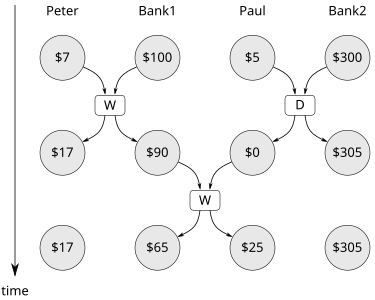
\includegraphics[width=94mm]{assets/figures/chapter_3/figure_3.30b.pdf}
\end{imageFigure}

A less stringent restriction on concurrency would ensure that a concurrent
system produces the same result as if the processes had run sequentially in
some order.  There are two important aspects to this requirement.  First, it
does not require the processes to actually run sequentially, but only to
produce results that are the same \emph{as if} they had run sequentially.  For
the example in \link{Figure 3.30}, the designer of the bank account system can
safely allow Paul's deposit and Peter's withdrawal to happen concurrently,
because the net result will be the same as if the two operations had happened
sequentially.  Second, there may be more than one possible ``correct'' result
produced by a concurrent program, because we require only that the result be
the same as for \emph{some} sequential order.  For example, suppose that Peter
and Paul's joint account starts out with \$100, and Peter deposits \$40 while
Paul concurrently withdraws half the money in the account.  Then sequential
execution could result in the account balance being either \$70 or \$90 (see
\link{Exercise 3.38}).\footnote{\label{Footnote 39} A more formal
way to express this idea is to say that concurrent programs are inherently
\newterm{nondeterministic}. That is, they are described not by single-valued
functions, but by functions whose results are sets of possible values.  In
\link{Section 4.3} we will study a language for expressing nondeterministic
computations.}

There are still weaker requirements for correct execution of concurrent
programs.  A program for simulating diffusion (say, the flow of heat in an
object) might consist of a large number of processes, each one representing a
small volume of space, that update their values concurrently.  Each process
repeatedly changes its value to the average of its own value and its neighbors'
values.  This algorithm converges to the right answer independent of the order
in which the operations are done; there is no need for any restrictions on
concurrent use of the shared values.

\begin{exerciseGroup}
\phantomsection\label{Exercise 3.38}
\exerciseHeading{Exercise 3.38:} Suppose that Peter, Paul, and
Mary share a joint bank account that initially contains \$100.  Concurrently,
Peter deposits \$10, Paul withdraws \$20, and Mary withdraws half the money in
the account, by executing the following commands:

\begin{codeBlock}
Peter: (set! balance (+ balance 10))
Paul:  (set! balance (- balance 20))
Mary:  (set! balance (- balance (/ balance 2)))
\end{codeBlock}

\begin{enumerate}[a.]

\item
List all the different possible values for \code{balance} after these three
transactions have been completed, assuming that the banking system forces the
three processes to run sequentially in some order.

\item
What are some other values that could be produced if the system allows the
processes to be interleaved?  Draw timing diagrams like the one in \link{Figure 3.29}
to explain how these values can occur.

\end{enumerate}
\end{exerciseGroup}

\subsection{Mechanisms for Controlling Concurrency}
\label{Section 3.4.2}

We've seen that the difficulty in dealing with concurrent processes is rooted
in the need to consider the interleaving of the order of events in the
different processes.  For example, suppose we have two processes, one with
three ordered events \( (a, b, c) \) and one with three ordered events
\( (x, y, z) \).  If the two processes run concurrently, with no
constraints on how their execution is interleaved, then there are 20 different
possible orderings for the events that are consistent with the individual
orderings for the two processes:

\begin{example}
(a,b,c,x,y,z)  (a,x,b,y,c,z)  (x,a,b,c,y,z)  (x,a,y,z,b,c)
(a,b,x,c,y,z)  (a,x,b,y,z,c)  (x,a,b,y,c,z)  (x,y,a,b,c,z)
(a,b,x,y,c,z)  (a,x,y,b,c,z)  (x,a,b,y,z,c)  (x,y,a,b,z,c)
(a,b,x,y,z,c)  (a,x,y,b,z,c)  (x,a,y,b,c,z)  (x,y,a,z,b,c)
(a,x,b,c,y,z)  (a,x,y,z,b,c)  (x,a,y,b,z,c)  (x,y,z,a,b,c)
\end{example}

\noindent
As programmers designing this system, we would have to consider the effects of
each of these 20 orderings and check that each behavior is acceptable.  Such an
approach rapidly becomes unwieldy as the numbers of processes and events
increase.

A more practical approach to the design of concurrent systems is to devise
general mechanisms that allow us to constrain the interleaving of concurrent
processes so that we can be sure that the program behavior is correct.  Many
mechanisms have been developed for this purpose.  In this section, we describe
one of them, the \newterm{serializer}.

\subsubsection*{Serializing access to shared state}

Serialization implements the following idea: Processes will execute
concurrently, but there will be certain collections of procedures that cannot
be executed concurrently.  More precisely, serialization creates distinguished
sets of procedures such that only one execution of a procedure in each
serialized set is permitted to happen at a time.  If some procedure in the set
is being executed, then a process that attempts to execute any procedure in the
set will be forced to wait until the first execution has finished.

We can use serialization to control access to shared variables.  For example,
if we want to update a shared variable based on the previous value of that
variable, we put the access to the previous value of the variable and the
assignment of the new value to the variable in the same procedure.  We then
ensure that no other procedure that assigns to the variable can run
concurrently with this procedure by serializing all of these procedures with
the same serializer.  This guarantees that the value of the variable cannot be
changed between an access and the corresponding assignment.

\subsubsection*{Serializers in Scheme}

To make the above mechanism more concrete, suppose that we have extended Scheme
to include a procedure called \code{parallel\-/execute}:

\begin{codeBlock}
(parallel-execute ~\(\langle \)~~\var{p}~~\(_{\mono{1}}\rangle \)~ ~\(\langle \)~~\var{p}~~\(_{\mono{2}}\rangle \)~ ~\( \dots \)~ ~\(\langle \)~~\var{p}~~\(_{\monoItalic{k}}\rangle \)~)
\end{codeBlock}

\noindent
Each \( \langle p \rangle \) must be a procedure of no arguments.  \code{parallel\-/execute}
creates a separate process for each \( \langle p \rangle \), which applies \( \langle p \rangle \) (to no
arguments).  These processes all run
concurrently.\footnote{\code{parallel\-/execute} is not part of standard Scheme,
but it can be implemented in \acronym{MIT} Scheme.  In our implementation, the
new concurrent processes also run concurrently with the original Scheme
process.  Also, in our implementation, the value returned by
\code{parallel\-/execute} is a special control object that can be used to halt
the newly created processes.}

As an example of how this is used, consider

\begin{codeBlock}
(define x 10)
(parallel-execute
 (lambda () (set! x (* x x)))
 (lambda () (set! x (+ x 1))))
\end{codeBlock}

\noindent
This creates two concurrent processes---\( P_1 \), which sets \code{x} to
\code{x} times \code{x}, and \( P_2 \), which increments \code{x}.  After
execution is complete, \code{x} will be left with one of five possible values,
depending on the interleaving of the events of \( P_1 \) and \( P_2 \):

\begin{codeBlock}
101: ~\textrm{\( P_1 \) sets \code{x} to 100 and then \( P_2 \) increments \code{x} to 101.}~
121: ~\textrm{\( P_2 \) increments \code{x} to 11 and then \( P_1 \) sets \code{x} to \code{x} \code{*} \code{x}.}~
110: ~\textrm{\( P_2 \) changes \code{x} from 10 to 11 between the two times that}~
     ~\textrm{\( P_1 \) accesses the value of \code{x} during the evaluation of \code{(* x x)}.}~
 11: ~\textrm{\( P_2 \) accesses \code{x}, then \( P_1 \) sets \code{x} to 100, then \( P_2 \) sets \code{x}.}~
100: ~\textrm{\( P_1 \) accesses \code{x} (twice), then \( P_2 \) sets \code{x} to 11, then \( P_1 \) sets \code{x}.}~
\end{codeBlock}

\noindent
We can constrain the concurrency by using serialized procedures, which are
created by \newterm{serializers}. Serializers are constructed by
\code{make\-/serializer}, whose implementation is given below.  A serializer
takes a procedure as argument and returns a serialized procedure that behaves
like the original procedure.  All calls to a given serializer return serialized
procedures in the same set.

Thus, in contrast to the example above, executing

\begin{codeBlock}
(define x 10)
(define s (make-serializer))
(parallel-execute
 (s (lambda () (set! x (* x x))))
 (s (lambda () (set! x (+ x 1)))))
\end{codeBlock}

\noindent
can produce only two possible values for \code{x}, 101 or 121.  The other
possibilities are eliminated, because the execution of \( P_1 \) and \( P_2 \)
cannot be interleaved.

Here is a version of the \code{make\-/account} procedure from
\link{Section 3.1.1}, where the deposits and withdrawals have been serialized:

\begin{codeBlock}
(define (make-account balance)
  (define (withdraw amount)
    (if (>= balance amount)
        (begin (set! balance (- balance amount))
          balance)
        "Insufficient funds"))
  (define (deposit amount)
    (set! balance (+ balance amount))
    balance)
  (let ((protected (make-serializer)))
    (define (dispatch m)
      (cond ((eq? m 'withdraw) (protected withdraw))
            ((eq? m 'deposit) (protected deposit))
            ((eq? m 'balance) balance)
            (else
              (error "Unknown request: MAKE-ACCOUNT"
                     m))))
    dispatch))
\end{codeBlock}

\noindent
With this implementation, two processes cannot be withdrawing from or
depositing into a single account concurrently.  This eliminates the source of
the error illustrated in \link{Figure 3.29}, where Peter changes the account
balance between the times when Paul accesses the balance to compute the new
value and when Paul actually performs the assignment.  On the other hand, each
account has its own serializer, so that deposits and withdrawals for different
accounts can proceed concurrently.

\begin{exerciseGroup}
\phantomsection\label{Exercise 3.39}
\exerciseHeading{Exercise 3.39:} Which of the five possibilities
in the parallel execution shown above remain if we instead serialize execution
as follows:

\begin{codeBlock}
(define x 10)
(define s (make-serializer))
(parallel-execute
 (lambda () (set! x ((s (lambda () (* x x))))))
 (s (lambda () (set! x (+ x 1)))))
\end{codeBlock}

\phantomsection\label{Exercise 3.40}
\exerciseHeading{Exercise 3.40:} Give all possible values of
\code{x} that can result from executing

\begin{codeBlock}
(define x 10)
(parallel-execute (lambda () (set! x (* x x)))
                  (lambda () (set! x (* x x x))))
\end{codeBlock}

Which of these possibilities remain if we instead use serialized procedures:

\begin{codeBlock}
(define x 10)
(define s (make-serializer))
(parallel-execute (s (lambda () (set! x (* x x))))
                  (s (lambda () (set! x (* x x x)))))
\end{codeBlock}

\phantomsection\label{Exercise 3.41}
\exerciseHeading{Exercise 3.41:} Ben Bitdiddle worries that it
would be better to implement the bank account as follows (where the commented
line has been changed):

\begin{codeBlock}
(define (make-account balance)
  (define (withdraw amount)
    (if (>= balance amount)
        (begin (set! balance
                     (- balance amount))
               balance)
        "Insufficient funds"))
  (define (deposit amount)
    (set! balance (+ balance amount))
    balance)
  (let ((protected (make-serializer)))
    (define (dispatch m)
      (cond ((eq? m 'withdraw) (protected withdraw))
            ((eq? m 'deposit) (protected deposit))
            ((eq? m 'balance)
             ((protected
               (lambda () balance)))) ~\textrm{; serialized}~
            (else
             (error "Unknown request: MAKE-ACCOUNT"
                    m))))
    dispatch))
\end{codeBlock}

\noindent
because allowing unserialized access to the bank balance can result in
anomalous behavior.  Do you agree?  Is there any scenario that demonstrates
Ben's concern?

\phantomsection\label{Exercise 3.42}
\exerciseHeading{Exercise 3.42:} Ben Bitdiddle suggests that it's
a waste of time to create a new serialized procedure in response to every
\code{withdraw} and \code{deposit} message.  He says that \code{make\-/account}
could be changed so that the calls to \code{protected} are done outside the
\code{dispatch} procedure.  That is, an account would return the same
serialized procedure (which was created at the same time as the account) each
time it is asked for a withdrawal procedure.

\begin{codeBlock}
(define (make-account balance)
  (define (withdraw amount)
    (if (>= balance amount)
        (begin (set! balance (- balance amount))
               balance)
        "Insufficient funds"))
  (define (deposit amount)
    (set! balance (+ balance amount))
    balance)
  (let ((protected (make-serializer)))
    (let ((protected-withdraw (protected withdraw))
          (protected-deposit (protected deposit)))
      (define (dispatch m)
        (cond ((eq? m 'withdraw) protected-withdraw)
              ((eq? m 'deposit) protected-deposit)
              ((eq? m 'balance) balance)
              (else
               (error "Unknown request: MAKE-ACCOUNT"
                      m))))
      dispatch)))
\end{codeBlock}

Is this a safe change to make?  In particular, is there any difference in what
concurrency is allowed by these two versions of \code{make\-/account}?
\end{exerciseGroup}

\subsubsection*{Complexity of using multiple shared resources}

Serializers provide a powerful abstraction that helps isolate the complexities
of concurrent programs so that they can be dealt with carefully and (hopefully)
correctly.  However, while using serializers is relatively straightforward when
there is only a single shared resource (such as a single bank account),
concurrent programming can be treacherously difficult when there are multiple
shared resources.

To illustrate one of the difficulties that can arise, suppose we wish to swap
the balances in two bank accounts.  We access each account to find the balance,
compute the difference between the balances, withdraw this difference from one
account, and deposit it in the other account.  We could implement this as
follows:\footnote{We have simplified \code{exchange} by exploiting the fact
that our \code{deposit} message accepts negative amounts.  (This is a serious
bug in our banking system!)}

\begin{codeBlock}
(define (exchange account1 account2)
  (let ((difference (- (account1 'balance)
                       (account2 'balance))))
    ((account1 'withdraw) difference)
    ((account2 'deposit) difference)))
\end{codeBlock}

\noindent
This procedure works well when only a single process is trying to do the
exchange.  Suppose, however, that Peter and Paul both have access to accounts
\( {a1} \), \( {a2} \), and \( {a3} \), and that Peter exchanges \( {a1} \)
and \( {a2} \) while Paul concurrently exchanges \( {a1} \) and \( {a3} \).  Even
with account deposits and withdrawals serialized for individual accounts (as in
the \code{make\-/account} procedure shown above in this section), \code{exchange}
can still produce incorrect results.  For example, Peter might compute the difference
in the balances for \( {a1} \) and \( {a2} \), but then Paul might change the balance
in \( {a1} \) before Peter is able to complete the exchange.\footnote{If the account
balances start out as \$10, \$20, and \$30, then after any number of concurrent
exchanges, the balances should still be \$10, \$20, and \$30 in some order.
Serializing the deposits to individual accounts is not sufficient to guarantee
this.  See \link{Exercise 3.43}.}  For correct behavior, we must arrange for the
\code{exchange} procedure to lock out any other concurrent accesses to the
accounts during the entire time of the exchange.

One way we can accomplish this is by using both accounts' serializers to
serialize the entire \code{exchange} procedure.  To do this, we will arrange
for access to an account's serializer.  Note that we are deliberately breaking
the modularity of the bank-account object by exposing the serializer.  The
following version of \code{make\-/account} is identical to the original version
given in \link{Section 3.1.1}, except that a serializer is provided to protect
the balance variable, and the serializer is exported via message passing:

\begin{codeBlock}
(define (make-account-and-serializer balance)
  (define (withdraw amount)
    (if (>= balance amount)
        (begin (set! balance (- balance amount))
          balance)
        "Insufficient funds"))
  (define (deposit amount)
    (set! balance (+ balance amount))
    balance)
  (let ((balance-serializer (make-serializer)))
    (define (dispatch m)
      (cond ((eq? m 'withdraw) withdraw)
            ((eq? m 'deposit) deposit)
            ((eq? m 'balance) balance)
            ((eq? m 'serializer) balance-serializer)
            (else
              (error "Unknown request: MAKE-ACCOUNT"
                     m))))
    dispatch))
\end{codeBlock}

\noindent
We can use this to do serialized deposits and withdrawals.  However, unlike our
earlier serialized account, it is now the responsibility of each user of
bank-account objects to explicitly manage the serialization, for example as
follows:\footnote{\link{Exercise 3.45} investigates why deposits and withdrawals
are no longer automatically serialized by the account.}

\begin{codeBlock}
(define (deposit account amount)
  (let ((s (account 'serializer))
        (d (account 'deposit)))
    ((s d) amount)))
\end{codeBlock}

\noindent
Exporting the serializer in this way gives us enough flexibility to implement a
serialized exchange program.  We simply serialize the original \code{exchange}
procedure with the serializers for both accounts:

\begin{codeBlock}
(define (serialized-exchange account1 account2)
  (let ((serializer1 (account1 'serializer))
        (serializer2 (account2 'serializer)))
    ((serializer1 (serializer2 exchange))
     account1
     account2)))
\end{codeBlock}

\begin{exerciseGroup}
\phantomsection\label{Exercise 3.43}
\exerciseHeading{Exercise 3.43:} Suppose that the balances in
three accounts start out as \$10, \$20, and \$30, and that multiple processes run,
exchanging the balances in the accounts.  Argue that if the processes are run
sequentially, after any number of concurrent exchanges, the account balances
should be \$10, \$20, and \$30 in some order.  Draw a timing diagram like the one
in \link{Figure 3.29} to show how this condition can be violated if the
exchanges are implemented using the first version of the account-exchange
program in this section.  On the other hand, argue that even with this
\code{exchange} program, the sum of the balances in the accounts will be
preserved.  Draw a timing diagram to show how even this condition would be
violated if we did not serialize the transactions on individual accounts.

\phantomsection\label{Exercise 3.44}
\exerciseHeading{Exercise 3.44:} Consider the problem of
transferring an amount from one account to another.  Ben Bitdiddle claims that
this can be accomplished with the following procedure, even if there are
multiple people concurrently transferring money among multiple accounts, using
any account mechanism that serializes deposit and withdrawal transactions, for
example, the version of \code{make\-/account} in the text above.

\begin{codeBlock}
(define (transfer from-account to-account amount)
  ((from-account 'withdraw) amount)
  ((to-account 'deposit) amount))
\end{codeBlock}

Louis Reasoner claims that there is a problem here, and that we need to use a
more sophisticated method, such as the one required for dealing with the
exchange problem.  Is Louis right?  If not, what is the essential difference
between the transfer problem and the exchange problem?  (You should assume that
the balance in \code{from\-/account} is at least \code{amount}.)

\phantomsection\label{Exercise 3.45}
\exerciseHeading{Exercise 3.45:} Louis Reasoner thinks our
bank-account system is unnecessarily complex and error-prone now that deposits
and withdrawals aren't automatically serialized.  He suggests that
\code{make\-/account\-/and\-/serializer} should have exported the serializer (for use
by such procedures as \code{serialized\-/exchange}) in addition to (rather than
instead of) using it to serialize accounts and deposits as \code{make\-/account}
did.  He proposes to redefine accounts as follows:

\begin{compactCodeBlock}
(define (make-account-and-serializer balance)
  (define (withdraw amount)
    (if (>= balance amount)
        (begin (set! balance (- balance amount)) balance)
        "Insufficient funds"))
  (define (deposit amount)
    (set! balance (+ balance amount)) balance)
  (let ((balance-serializer (make-serializer)))
    (define (dispatch m)
      (cond ((eq? m 'withdraw) (balance-serializer withdraw))
            ((eq? m 'deposit) (balance-serializer deposit))
            ((eq? m 'balance) balance)
            ((eq? m 'serializer) balance-serializer)
            (else (error "Unknown request: MAKE-ACCOUNT" m))))
    dispatch))
\end{compactCodeBlock}

Then deposits are handled as with the original \code{make\-/account}:

\begin{codeBlock}
(define (deposit account amount)
  ((account 'deposit) amount))
\end{codeBlock}

Explain what is wrong with Louis's reasoning.  In particular, consider what
happens when \code{serialized\-/exchange} is called.
\end{exerciseGroup}

\subsubsection*{Implementing serializers}

We implement serializers in terms of a more primitive synchronization mechanism
called a \newterm{mutex}.  A mutex is an object that supports two
operations---the mutex can be \newterm{acquired}, and the mutex can be
\newterm{released}.  Once a mutex has been acquired, no other acquire
operations on that mutex may proceed until the mutex is released.\footnote{The
term ``mutex'' is an abbreviation for \newterm{mutual exclusion}.  The general
problem of arranging a mechanism that permits concurrent processes to safely
share resources is called the mutual exclusion problem.  Our mutex is a simple
variant of the \newterm{semaphore} mechanism (see \link{Exercise 3.47}), which
was introduced in the ``THE'' Multiprogramming System developed at the
Technological University of Eindhoven and named for the university's initials
in Dutch (\link{Dijkstra 1968a}).  The acquire and release operations were originally
called P and V, from the Dutch words \emph{passeren} (to pass) and
\emph{vrijgeven} (to release), in reference to the semaphores used on railroad
systems.  Dijkstra's classic exposition (\link{Dijkstra 1968b}) was one of the first to clearly
present the issues of concurrency control, and showed how to use semaphores to
handle a variety of concurrency problems.} In our implementation, each
serializer has an associated mutex.  Given a procedure \code{p}, the serializer
returns a procedure that acquires the mutex, runs \code{p}, and then releases
the mutex.  This ensures that only one of the procedures produced by the
serializer can be running at once, which is precisely the serialization
property that we need to guarantee.

\begin{codeBlock}
(define (make-serializer)
  (let ((mutex (make-mutex)))
    (lambda (p)
      (define (serialized-p . args)
        (mutex 'acquire)
        (let ((val (apply p args)))
          (mutex 'release)
          val))
      serialized-p)))
\end{codeBlock}

\noindent
The mutex is a mutable object (here we'll use a one-element list, which we'll
refer to as a \newterm{cell}) that can hold the value true or false.  When the
value is false, the mutex is available to be acquired.  When the value is true,
the mutex is unavailable, and any process that attempts to acquire the mutex
must wait.

Our mutex constructor \code{make\-/mutex} begins by initializing the cell
contents to false.  To acquire the mutex, we test the cell.  If the mutex is
available, we set the cell contents to true and proceed.  Otherwise, we wait in
a loop, attempting to acquire over and over again, until we find that the mutex
is available.\footnote{In most time-shared operating systems, processes that
are blocked by a mutex do not waste time ``busy-waiting'' as above.  Instead,
the system schedules another process to run while the first is waiting, and the
blocked process is awakened when the mutex becomes available.}  To release the
mutex, we set the cell contents to false.

\begin{codeBlock}
(define (make-mutex)
  (let ((cell (list false)))
    (define (the-mutex m)
      (cond ((eq? m 'acquire)
             (if (test-and-set! cell)
                 (the-mutex 'acquire))) ~\textrm{; retry}~
            ((eq? m 'release) (clear! cell))))
    the-mutex))
(define (clear! cell) (set-car! cell false))
\end{codeBlock}

\noindent
\code{test\-/and\-/set!} tests the cell and returns the result of the test.  In
addition, if the test was false, \code{test\-/and\-/set!} sets the cell contents to
true before returning false.  We can express this behavior as the following
procedure:

\begin{codeBlock}
(define (test-and-set! cell)
  (if (car cell) true (begin (set-car! cell true) false)))
\end{codeBlock}

\noindent
However, this implementation of \code{test\-/and\-/set!} does not suffice as it
stands.  There is a crucial subtlety here, which is the essential place where
concurrency control enters the system: The \code{test\-/and\-/set!} operation must
be performed \newterm{atomically}.  That is, we must guarantee that, once a
process has tested the cell and found it to be false, the cell contents will
actually be set to true before any other process can test the cell.  If we do
not make this guarantee, then the mutex can fail in a way similar to the
bank-account failure in \link{Figure 3.29}.  (See \link{Exercise 3.46}.)

The actual implementation of \code{test\-/and\-/set!} depends on the details of how
our system runs concurrent processes.  For example, we might be executing
concurrent processes on a sequential processor using a time-slicing mechanism
that cycles through the processes, permitting each process to run for a short
time before interrupting it and moving on to the next process.  In that case,
\code{test\-/and\-/set!}  can work by disabling time slicing during the testing and
setting.\footnote{In \acronym{MIT} Scheme for a single processor, which uses a
time-slicing model, \code{test\-/and\-/set!} can be implemented as follows:

\begin{compactCodeBlock}
(define (test-and-set! cell)
  (without-interrupts
   (lambda ()
     (if (car cell)
         true
         (begin (set-car! cell true)
                false)))))
\end{compactCodeBlock}

\noindent
\code{without\-/interrupts} disables time-slicing interrupts while its procedure
argument is being executed.}  Alternatively, multiprocessing computers provide
instructions that support atomic operations directly in
hardware.\footnote{There are many variants of such instructions---including
test-and-set, test-and-clear, swap, compare-and-exchange, load-reserve, and
store-conditional---whose design must be carefully matched to the machine's
processor-memory interface.  One issue that arises here is to determine what
happens if two processes attempt to acquire the same resource at exactly the
same time by using such an instruction.  This requires some mechanism for
making a decision about which process gets control.  Such a mechanism is called
an \newterm{arbiter}.  Arbiters usually boil down to some sort of hardware
device.  Unfortunately, it is possible to prove that one cannot physically
construct a fair arbiter that works 100\% of the time unless one allows the
arbiter an arbitrarily long time to make its decision.  The fundamental
phenomenon here was originally observed by the fourteenth-century French
philosopher Jean Buridan in his commentary on Aristotle's \textit{De caelo}.
Buridan argued that a perfectly rational dog placed between two equally
attractive sources of food will starve to death, because it is incapable of
deciding which to go to first.}

\begin{exerciseGroup}
\phantomsection\label{Exercise 3.46}
\exerciseHeading{Exercise 3.46:} Suppose that we implement
\code{test\-/and\-/set!}  using an ordinary procedure as shown in the text, without
attempting to make the operation atomic.  Draw a timing diagram like the one in
\link{Figure 3.29} to demonstrate how the mutex implementation can fail by
allowing two processes to acquire the mutex at the same time.

\phantomsection\label{Exercise 3.47}
\exerciseHeading{Exercise 3.47:} A semaphore (of size \( n \)) is a
generalization of a mutex.  Like a mutex, a semaphore supports acquire and
release operations, but it is more general in that up to \( n \) processes can
acquire it concurrently.  Additional processes that attempt to acquire the
semaphore must wait for release operations.  Give implementations of semaphores

\begin{enumerate}[a.]

\item
in terms of mutexes

\item
in terms of atomic \code{test\-/and\-/set!} operations.

\end{enumerate}
\end{exerciseGroup}

\subsubsection*{Deadlock}

Now that we have seen how to implement serializers, we can see that account
exchanging still has a problem, even with the \code{serialized\-/exchange}
procedure above.  Imagine that Peter attempts to exchange \( a1 \) with \( a2 \)
while Paul concurrently attempts to exchange \( a2 \) with \( a1 \).  Suppose that
Peter's process reaches the point where it has entered a serialized procedure
protecting \( a1 \) and, just after that, Paul's process enters a serialized
procedure protecting \( a2 \).  Now Peter cannot proceed (to enter a serialized
procedure protecting \( a2 \)) until Paul exits the serialized procedure
protecting \( a2 \).  Similarly, Paul cannot proceed until Peter exits the
serialized procedure protecting \( a1 \).  Each process is stalled forever,
waiting for the other.  This situation is called a \newterm{deadlock}.
Deadlock is always a danger in systems that provide concurrent access to
multiple shared resources.

One way to avoid the deadlock in this situation is to give each account a
unique identification number and rewrite \code{serialized\-/exchange} so that a
process will always attempt to enter a procedure protecting the lowest-numbered
account first.  Although this method works well for the exchange problem, there
are other situations that require more sophisticated deadlock-avoidance
techniques, or where deadlock cannot be avoided at all.  (See \link{Exercise 3.48}
and \link{Exercise 3.49}.)\footnote{The general technique for avoiding
deadlock by numbering the shared resources and acquiring them in order is due
to \link{Havender (1968)}.  Situations where deadlock cannot be avoided require
\newterm{deadlock-recovery} methods, which entail having processes ``back out''
of the deadlocked state and try again.  Deadlock-recovery mechanisms are widely
used in database management systems, a topic that is treated in detail in
\link{Gray and Reuter 1993}.}

\begin{exerciseGroup}
\phantomsection\label{Exercise 3.48}
\exerciseHeading{Exercise 3.48:} Explain in detail why the
deadlock-avoidance method described above, (i.e., the accounts are numbered,
and each process attempts to acquire the smaller-numbered account first) avoids
deadlock in the exchange problem.  Re\-write \code{serialized\-/exchange} to
incorporate this idea.  (You will also need to modify \code{make\-/account} so
that each account is created with a number, which can be accessed by sending an
appropriate message.)

\phantomsection\label{Exercise 3.49}
\exerciseHeading{Exercise 3.49:} Give a scenario where the
deadlock-avoid\-ance mechanism described above does not work.  (Hint: In the
exchange problem, each process knows in advance which accounts it will need to
get access to.  Consider a situation where a process must get access to some
shared resources before it can know which additional shared resources it will
require.)
\end{exerciseGroup}

\subsubsection*{Concurrency, time, and communication}

We've seen how programming concurrent systems requires controlling the ordering
of events when different processes access shared state, and we've seen how to
achieve this control through judicious use of serializers.  But the problems of
concurrency lie deeper than this, because, from a fundamental point of view,
it's not always clear what is meant by ``shared state.''

Mechanisms such as \code{test\-/and\-/set!} require processes to examine a global
shared flag at arbitrary times.  This is problematic and inefficient to
implement in modern high-speed processors, where due to optimization techniques
such as pipelining and cached memory, the contents of memory may not be in a
consistent state at every instant.  In contemporary multiprocessing systems,
therefore, the serializer paradigm is being supplanted by new approaches to
concurrency control.\footnote{One such alternative to serialization is called
\newterm{barrier synchronization}.  The programmer permits concurrent processes
to execute as they please, but establishes certain synchronization points
(``barriers'') through which no process can proceed until all the processes
have reached the barrier.  Modern processors provide machine instructions that
permit programmers to establish synchronization points at places where
consistency is required.  The PowerPC, for example, includes for
this purpose two instructions called \acronym{SYNC} and \acronym{EIEIO}
(Enforced In-order Execution of Input/Output).}

The problematic aspects of shared state also arise in large, distributed
systems.  For instance, imagine a distributed banking system where individual
branch banks maintain local values for bank balances and periodically compare
these with values maintained by other branches.  In such a system the value of
``the account balance'' would be undetermined, except right after
synchronization.  If Peter deposits money in an account he holds jointly with
Paul, when should we say that the account balance has changed---when the
balance in the local branch changes, or not until after the synchronization?
And if Paul accesses the account from a different branch, what are the
reasonable constraints to place on the banking system such that the behavior is
``correct''?  The only thing that might matter for correctness is the behavior
observed by Peter and Paul individually and the ``state'' of the account
immediately after synchronization.  Questions about the ``real'' account
balance or the order of events between synchronizations may be irrelevant or
meaningless.\footnote{This may seem like a strange point of view, but there are
systems that work this way.  International charges to credit-card accounts, for
example, are normally cleared on a per-country basis, and the charges made in
different countries are periodically reconciled.  Thus the account balance may
be different in different countries.}

The basic phenomenon here is that synchronizing different processes,
establishing shared state, or imposing an order on events requires
communication among the processes.  In essence, any notion of time in
concurrency control must be intimately tied to communication.\footnote{For
distributed systems, this perspective was pursued by \link{Lamport (1978)}, who showed
how to use communication to establish ``global clocks'' that can be used to
establish orderings on events in distributed systems.}  It is intriguing that a
similar connection between time and communication also arises in the Theory of
Relativity, where the speed of light (the fastest signal that can be used to
synchronize events) is a fundamental constant relating time and space.  The
complexities we encounter in dealing with time and state in our computational
models may in fact mirror a fundamental complexity of the physical universe.

\section{Streams}
\label{Section 3.5}

We've gained a good understanding of assignment as a tool in modeling, as well
as an appreciation of the complex problems that assignment raises. It is time
to ask whether we could have gone about things in a different way, so as to
avoid some of these problems.  In this section, we explore an alternative
approach to modeling state, based on data structures called \newterm{streams}.
As we shall see, streams can mitigate some of the complexity of modeling state.

Let's step back and review where this complexity comes from.  In an attempt to
model real-world phenomena, we made some apparently reasonable decisions: We
modeled real-world objects with local state by computational objects with local
variables.  We identified time variation in the real world with time variation
in the computer.  We implemented the time variation of the states of the model
objects in the computer with assignments to the local variables of the model
objects.

Is there another approach?  Can we avoid identifying time in the computer with
time in the modeled world?  Must we make the model change with time in order to
model phenomena in a changing world?  Think about the issue in terms of
mathematical functions.  We can describe the time-varying behavior of a
quantity \( x \) as a function of time \( x(t) \).  If we concentrate on \( x \)
instant by instant, we think of it as a changing quantity.  Yet if we
concentrate on the entire time history of values, we do not emphasize
change---the function itself does not change.\footnote{Physicists sometimes
adopt this view by introducing the ``world lines'' of particles as a device for
reasoning about motion.  We've also already mentioned (\link{Section 2.2.3})
that this is the natural way to think about signal-processing systems.  We will
explore applications of streams to signal processing in \link{Section 3.5.3}.}

If time is measured in discrete steps, then we can model a time function as a
(possibly infinite) sequence.  In this section, we will see how to model change
in terms of sequences that represent the time histories of the systems being
modeled.  To accomplish this, we introduce new data structures called
\newterm{streams}.  From an abstract point of view, a stream is simply a
sequence.  However, we will find that the straightforward implementation of
streams as lists (as in \link{Section 2.2.1}) doesn't fully reveal the power of
stream processing.  As an alternative, we introduce the technique of
\newterm{delayed evaluation}, which enables us to represent very large (even
infinite) sequences as streams.

Stream processing lets us model systems that have state without ever using
assignment or mutable data.  This has important implications, both theoretical
and practical, because we can build models that avoid the drawbacks inherent in
introducing assignment.  On the other hand, the stream framework raises
difficulties of its own, and the question of which modeling technique leads to
more modular and more easily maintained systems remains open.



\subsection{Streams Are Delayed Lists}
\label{Section 3.5.1}

As we saw in \link{Section 2.2.3}, sequences can serve as standard interfaces
for combining program modules.  We formulated powerful abstractions for
manipulating sequences, such as \code{map}, \code{filter}, and
\code{accumulate}, that capture a wide variety of operations in a manner that
is both succinct and elegant.

Unfortunately, if we represent sequences as lists, this elegance is bought at
the price of severe inefficiency with respect to both the time and space
required by our computations.  When we represent manipulations on sequences as
transformations of lists, our programs must construct and copy data structures
(which may be huge) at every step of a process.

To see why this is true, let us compare two programs for computing the sum of
all the prime numbers in an interval.  The first program is written in standard
iterative style:\footnote{Assume that we have a predicate \code{prime?} (e.g.,
as in \link{Section 1.2.6}) that tests for primality.}

\begin{codeBlock}
(define (sum-primes a b)
  (define (iter count accum)
    (cond ((> count b) accum)
          ((prime? count)
             (iter (+ count 1) (+ count accum)))
          (else (iter (+ count 1) accum))))
  (iter a 0))
\end{codeBlock}

\noindent
The second program performs the same computation using the sequence operations
of \link{Section 2.2.3}:

\begin{codeBlock}
(define (sum-primes a b)
  (accumulate +
              0
              (filter prime?
                      (enumerate-interval a b))))
\end{codeBlock}

\noindent
In carrying out the computation, the first program needs to store only the sum
being accumulated.  In contrast, the filter in the second program cannot do any
testing until \code{enumerate\-/interval} has constructed a complete list of the
numbers in the interval.  The filter generates another list, which in turn is
passed to \code{accumulate} before being collapsed to form a sum.  Such large
intermediate storage is not needed by the first program, which we can think of
as enumerating the interval incrementally, adding each prime to the sum as it
is generated.

The inefficiency in using lists becomes painfully apparent if we use the
sequence paradigm to compute the second prime in the interval from 10,000 to
1,000,000 by evaluating the expression

\begin{codeBlock}
(car (cdr (filter prime?
                  (enumerate-interval 10000 1000000))))
\end{codeBlock}

\noindent
This expression does find the second prime, but the computational overhead is
outrageous.  We construct a list of almost a million integers, filter this list
by testing each element for primality, and then ignore almost all of the
result.  In a more traditional programming style, we would interleave the
enumeration and the filtering, and stop when we reached the second prime.

Streams are a clever idea that allows one to use sequence manipulations without
incurring the costs of manipulating sequences as lists.  With streams we can
achieve the best of both worlds: We can formulate programs elegantly as
sequence manipulations, while attaining the efficiency of incremental
computation.  The basic idea is to arrange to construct a stream only
partially, and to pass the partial construction to the program that consumes
the stream.  If the consumer attempts to access a part of the stream that has
not yet been constructed, the stream will automatically construct just enough
more of itself to produce the required part, thus preserving the illusion that
the entire stream exists.  In other words, although we will write programs as
if we were processing complete sequences, we design our stream implementation
to automatically and transparently interleave the construction of the stream
with its use.

On the surface, streams are just lists with different names for the procedures
that manipulate them.  There is a constructor, \code{cons\-/stream}, and two
selectors, \code{stream\-/car} and \code{stream\-/cdr}, which satisfy the
constraints

\begin{codeBlock}
(stream-car (cons-stream x y)) = x
(stream-cdr (cons-stream x y)) = y
\end{codeBlock}

\noindent
There is a distinguishable object, \code{the\-/empty\-/stream}, which cannot be the
result of any \code{cons\-/stream} operation, and which can be identified with
the predicate \code{stream\-/null?}.\footnote{In the \acronym{MIT}
implementation, \code{the\-/empty\-/stream} is the same as the empty list
\code{'()}, and \code{stream\-/null?} is the same as \code{null?}.}  Thus we can
make and use streams, in just the same way as we can make and use lists, to
represent aggregate data arranged in a sequence.  In particular, we can build
stream analogs of the list operations from \link{Chapter 2}, such as
\code{list\-/ref}, \code{map}, and \code{for\-/each}:\footnote{This should bother
you.  The fact that we are defining such similar procedures for streams and
lists indicates that we are missing some underlying abstraction.
Unfortunately, in order to exploit this abstraction, we will need to exert
finer control over the process of evaluation than we can at present.  We will
discuss this point further at the end of \link{Section 3.5.4}.  In
\link{Section 4.2}, we'll develop a framework that unifies lists and streams.}

\begin{codeBlock}
(define (stream-ref s n)
  (if (= n 0)
      (stream-car s)
      (stream-ref (stream-cdr s) (- n 1))))
(define (stream-map proc s)
  (if (stream-null? s)
      the-empty-stream
      (cons-stream (proc (stream-car s))
                   (stream-map proc (stream-cdr s)))))
(define (stream-for-each proc s)
  (if (stream-null? s)
      'done
      (begin (proc (stream-car s))
             (stream-for-each proc (stream-cdr s)))))
\end{codeBlock}

\noindent
\code{stream\-/for\-/each} is useful for viewing streams:

\begin{codeBlock}
(define (display-stream s)
  (stream-for-each display-line s))
(define (display-line x) (newline) (display x))
\end{codeBlock}

\noindent
To make the stream implementation automatically and transparently interleave
the construction of a stream with its use, we will arrange for the \code{cdr}
of a stream to be evaluated when it is accessed by the \code{stream\-/cdr}
procedure rather than when the stream is constructed by \code{cons\-/stream}.
This implementation choice is reminiscent of our discussion of rational numbers
in \link{Section 2.1.2}, where we saw that we can choose to implement rational
numbers so that the reduction of numerator and denominator to lowest terms is
performed either at construction time or at selection time.  The two
rational-number implementations produce the same data abstraction, but the
choice has an effect on efficiency.  There is a similar relationship between
streams and ordinary lists.  As a data abstraction, streams are the same as
lists.  The difference is the time at which the elements are evaluated.  With
ordinary lists, both the \code{car} and the \code{cdr} are evaluated at
construction time.  With streams, the \code{cdr} is evaluated at selection
time.

Our implementation of streams will be based on a special form called
\code{delay}.  Evaluating \code{(delay \( \langle \)\var{exp}\( \rangle \))} does not evaluate the
expression \( \langle \)\var{exp}\( \kern0.08em\rangle \), but rather returns a so-called \newterm{delayed
object}, which we can think of as a ``promise'' to evaluate \( \langle \)\var{exp}\( \kern0.08em\rangle \) at some
future time.  As a companion to \code{delay}, there is a procedure called
\code{force} that takes a delayed object as argument and performs the
evaluation---in effect, forcing the \code{delay} to fulfill its promise.  We
will see below how \code{delay} and \code{force} can be implemented, but first
let us use these to construct streams.

\code{cons\-/stream} is a special form defined so that

\begin{codeBlock}
(cons-stream ~\(\langle \)~~\var{a}~~\(\rangle \)~ ~\(\langle \)~~\var{b}~~\(\rangle \)~)
\end{codeBlock}

\noindent
is equivalent to

\begin{codeBlock}
(cons ~\(\langle \)~~\var{a}~~\(\rangle \)~ (delay ~\(\langle \)~~\var{b}~~\(\rangle \)~))
\end{codeBlock}

\noindent
What this means is that we will construct streams using pairs.  However, rather
than placing the value of the rest of the stream into the \code{cdr} of the
pair we will put there a promise to compute the rest if it is ever requested.
\code{stream\-/car} and \code{stream\-/cdr} can now be defined as procedures:

\begin{codeBlock}
(define (stream-car stream) (car stream))
(define (stream-cdr stream) (force (cdr stream)))
\end{codeBlock}

\noindent
\code{stream\-/car} selects the \code{car} of the pair; \code{stream\-/cdr} selects
the \code{cdr} of the pair and evaluates the delayed expression found there to
obtain the rest of the stream.\footnote{Although \code{stream\-/car} and
\code{stream\-/cdr} can be defined as procedures, \code{cons\-/stream} must be a
special form.  If \code{cons\-/stream} were a procedure, then, according to our
model of evaluation, evaluating \code{(cons\-/stream \( \langle \)\var{a}\( \rangle \) \( \langle \)\var{b}\( \rangle \))} would
automatically cause \( \langle \)\var{b}\( \kern0.08em\rangle \) to be evaluated, which is precisely what we do
not want to happen.  For the same reason, \code{delay} must be a special form,
though \code{force} can be an ordinary procedure.}

\subsubsection*{The stream implementation in action}

To see how this implementation behaves, let us analyze the ``outrageous'' prime
computation we saw above, reformulated in terms of streams:

\begin{codeBlock}
(stream-car
 (stream-cdr
  (stream-filter prime?
                 (stream-enumerate-interval
                  10000 1000000))))
\end{codeBlock}

\noindent
We will see that it does indeed work efficiently.

We begin by calling \code{stream\-/enumerate\-/interval} with the arguments 10,000
and 1,000,000.  \code{stream\-/enumerate\-/interval} is the stream analog of
\code{enumerate\-/interval} (\link{Section 2.2.3}):

\begin{codeBlock}
(define (stream-enumerate-interval low high)
  (if (> low high)
      the-empty-stream
      (cons-stream
       low
       (stream-enumerate-interval (+ low 1) high))))
\end{codeBlock}

\noindent
and thus the result returned by \code{stream\-/enumerate\-/interval}, formed by the
\code{cons\-/stream}, is\footnote{The numbers shown here do not really appear in
the delayed expression.  What actually appears is the original expression, in
an environment in which the variables are bound to the appropriate numbers.
For example, \code{(+ low 1)} with \code{low} bound to 10,000 actually appears
where \code{10001} is shown.}

\begin{codeBlock}
(cons 10000
      (delay (stream-enumerate-interval 10001 1000000)))
\end{codeBlock}

\noindent
That is, \code{stream\-/enumerate\-/interval} returns a stream represented as a
pair whose \code{car} is 10,000 and whose \code{cdr} is a promise to enumerate
more of the interval if so requested.  This stream is now filtered for primes,
using the stream analog of the \code{filter} procedure (\link{Section 2.2.3}):

\begin{codeBlock}
(define (stream-filter pred stream)
  (cond ((stream-null? stream) the-empty-stream)
        ((pred (stream-car stream))
         (cons-stream (stream-car stream)
                      (stream-filter
                       pred
                       (stream-cdr stream))))
        (else (stream-filter pred (stream-cdr stream)))))
\end{codeBlock}

\noindent
\code{stream\-/filter} tests the \code{stream\-/car} of the stream (the \code{car}
of the pair, which is 10,000).  Since this is not prime, \code{stream\-/filter}
examines the \code{stream\-/cdr} of its input stream.  The call to
\code{stream\-/cdr} forces evaluation of the delayed
\code{stream\-/enumerate\-/interval}, which now returns

\begin{codeBlock}
(cons 10001
      (delay (stream-enumerate-interval 10002 1000000)))
\end{codeBlock}

\noindent
\code{stream\-/filter} now looks at the \code{stream\-/car} of this stream, 10,001,
sees that this is not prime either, forces another \code{stream\-/cdr}, and so
on, until \code{stream\-/enumerate\-/interval} yields the prime 10,007, whereupon
\code{stream\-/filter}, according to its definition, returns

\begin{codeBlock}
(cons-stream (stream-car stream)
             (stream-filter pred (stream-cdr stream)))
\end{codeBlock}

\noindent
which in this case is

\begin{codeBlock}
(cons 10007
      (delay (stream-filter
              prime?
              (cons 10008
                    (delay (stream-enumerate-interval
                            10009
                            1000000))))))
\end{codeBlock}

\noindent
This result is now passed to \code{stream\-/cdr} in our original expression.
This forces the delayed \code{stream\-/filter}, which in turn keeps forcing the
delayed \code{stream\-/enumerate\-/interval} until it finds the next prime, which
is 10,009.  Finally, the result passed to \code{stream\-/car} in our original
expression is

\begin{codeBlock}
(cons 10009
      (delay (stream-filter
              prime?
              (cons 10010
                    (delay (stream-enumerate-interval
                            10011
                            1000000))))))
\end{codeBlock}

\noindent
\code{stream\-/car} returns 10,009, and the computation is complete.  Only as
many integers were tested for primality as were necessary to find the second
prime, and the interval was enumerated only as far as was necessary to feed the
prime filter.

In general, we can think of delayed evaluation as ``demand-driven''
programming, whereby each stage in the stream process is activated only enough
to satisfy the next stage.  What we have done is to decouple the actual order
of events in the computation from the apparent structure of our procedures.  We
write procedures as if the streams existed ``all at once'' when, in reality,
the computation is performed incrementally, as in traditional programming
styles.

\subsubsection*{Implementing \code{delay} and \code{force}}

Although \code{delay} and \code{force} may seem like mysterious operations,
their implementation is really quite straightforward.  \code{delay} must
package an expression so that it can be evaluated later on demand, and we can
accomplish this simply by treating the expression as the body of a procedure.
\code{delay} can be a special form such that

\begin{codeBlock}
(delay ~\(\langle \)~~\var{exp}~~\(\rangle \)~)
\end{codeBlock}

\noindent
is syntactic sugar for

\begin{codeBlock}
(lambda () ~\(\langle \)~~\var{exp}~~\(\rangle \)~)
\end{codeBlock}

\noindent
\code{force} simply calls the procedure (of no arguments) produced by
\code{delay}, so we can implement \code{force} as a procedure:

\begin{codeBlock}
(define (force delayed-object) (delayed-object))
\end{codeBlock}

\noindent
This implementation suffices for \code{delay} and \code{force} to work as
advertised, but there is an important optimization that we can include.  In
many applications, we end up forcing the same delayed object many times.  This
can lead to serious inefficiency in recursive programs involving streams.  (See
\link{Exercise 3.57}.)  The solution is to build delayed objects so that the
first time they are forced, they store the value that is computed.  Subsequent
forcings will simply return the stored value without repeating the computation.
In other words, we implement \code{delay} as a special-purpose memoized
procedure similar to the one described in \link{Exercise 3.27}.  One way to
accomplish this is to use the following procedure, which takes as argument a
procedure (of no arguments) and returns a memoized version of the procedure.
The first time the memoized procedure is run, it saves the computed result.  On
subsequent evaluations, it simply returns the result.

\begin{codeBlock}
(define (memo-proc proc)
  (let ((already-run? false) (result false))
    (lambda ()
      (if (not already-run?)
          (begin (set! result (proc))
                 (set! already-run? true)
                 result)
          result))))
\end{codeBlock}

\noindent
\code{delay} is then defined so that \code{(delay \( \langle \)\var{exp}\( \rangle \))} is equivalent
to

\begin{codeBlock}
(memo-proc (lambda () ~\(\langle \)~~\var{exp}~~\(\rangle \)~))
\end{codeBlock}

\noindent
and \code{force} is as defined previously.\footnote{There are many possible
implementations of streams other than the one described in this section.
Delayed evaluation, which is the key to making streams practical, was inherent
in Algol 60's \newterm{call-by-name} parameter-passing method.  The use of this
mechanism to implement streams was first described by \link{Landin (1965)}.  Delayed
evaluation for streams was introduced into Lisp by \link{Friedman and Wise (1976)}. In
their implementation, \code{cons} always delays evaluating its arguments, so
that lists automatically behave as streams.  The memoizing optimization is also
known as \newterm{call-by-need}.  The Algol community would refer to our
original delayed objects as \newterm{call-by-name thunks} and to the optimized
versions as \newterm{call-by-need thunks}.}

\begin{exerciseGroup}
\phantomsection\label{Exercise 3.50}
\exerciseHeading{Exercise 3.50:} Complete the following
definition, which generalizes \code{stream\-/map} to allow procedures that take
multiple arguments, analogous to \code{map} in \link{Section 2.2.1},
\link{Footnote 12}.

\begin{codeBlock}
(define (stream-map proc . argstreams)
  (if (~\(\langle \)~??~\(\rangle \)~ (car argstreams))
      the-empty-stream
      (~\(\langle \)~??~\(\rangle \)~
       (apply proc (map ~\(\langle \)~??~\(\rangle \)~ argstreams))
       (apply stream-map
              (cons proc (map ~\(\langle \)~??~\(\rangle \)~ argstreams))))))
\end{codeBlock}

\phantomsection\label{Exercise 3.51}
\exerciseHeading{Exercise 3.51:} In order to take a closer look at
delayed evaluation, we will use the following procedure, which simply returns
its argument after printing it:

\begin{codeBlock}
(define (show x)
  (display-line x)
  x)
\end{codeBlock}

What does the interpreter print in response to evaluating each expression in
the following sequence?\footnote{Exercises such as \link{Exercise 3.51} and
\link{Exercise 3.52} are valuable for testing our understanding of how
\code{delay} works.  On the other hand, intermixing delayed evaluation with
printing---and, even worse, with assignment---is extremely confusing, and
instructors of courses on computer languages have traditionally tormented their
students with examination questions such as the ones in this section.  Needless
to say, writing programs that depend on such subtleties is odious programming
style.  Part of the power of stream processing is that it lets us ignore the
order in which events actually happen in our programs.  Unfortunately, this is
precisely what we cannot afford to do in the presence of assignment, which
forces us to be concerned with time and change.}

\begin{codeBlock}
(define x
  (stream-map show
              (stream-enumerate-interval 0 10)))
(stream-ref x 5)
(stream-ref x 7)
\end{codeBlock}

\phantomsection\label{Exercise 3.52}
\exerciseHeading{Exercise 3.52:} Consider the sequence of
expressions

\begin{codeBlock}
(define sum 0)
(define (accum x) (set! sum (+ x sum)) sum)
(define seq
  (stream-map accum
              (stream-enumerate-interval 1 20)))
(define y (stream-filter even? seq))
(define z
  (stream-filter (lambda (x) (= (remainder x 5) 0))
                 seq))
(stream-ref y 7)
(display-stream z)
\end{codeBlock}

What is the value of \code{sum} after each of the above expressions is
evaluated?  What is the printed response to evaluating the \code{stream\-/ref}
and \code{display\-/stream} expressions?  Would these responses differ if we had
implemented \code{(delay \( \langle \)\var{exp}\( \rangle \))} simply as
\code{(lambda () \( \langle \)\var{exp}\( \rangle \))}
without using the optimization provided by \code{memo\-/proc}?  Explain.
\end{exerciseGroup}

\subsection{Infinite Streams}
\label{Section 3.5.2}

We have seen how to support the illusion of manipulating streams as complete
entities even though, in actuality, we compute only as much of the stream as we
need to access.  We can exploit this technique to represent sequences
efficiently as streams, even if the sequences are very long.  What is more
striking, we can use streams to represent sequences that are infinitely long.
For instance, consider the following definition of the stream of positive
integers:

\begin{codeBlock}
(define (integers-starting-from n)
  (cons-stream n (integers-starting-from (+ n 1))))
(define integers (integers-starting-from 1))
\end{codeBlock}

\noindent
This makes sense because \code{integers} will be a pair whose \code{car} is 1
and whose \code{cdr} is a promise to produce the integers beginning with 2.
This is an infinitely long stream, but in any given time we can examine only a
finite portion of it.  Thus, our programs will never know that the entire
infinite stream is not there.

Using \code{integers} we can define other infinite streams, such as the stream
of integers that are not divisible by 7:

\begin{codeBlock}
(define (divisible? x y) (= (remainder x y) 0))
(define no-sevens
  (stream-filter (lambda (x) (not (divisible? x 7)))
                 integers))
\end{codeBlock}

\noindent
Then we can find integers not divisible by 7 simply by accessing elements of
this stream:

\begin{codeBlock}
(stream-ref no-sevens 100)
~\textit{117}~
\end{codeBlock}

\noindent
In analogy with \code{integers}, we can define the infinite stream of Fibonacci
numbers:

\begin{codeBlock}
(define (fibgen a b) (cons-stream a (fibgen b (+ a b))))
(define fibs (fibgen 0 1))
\end{codeBlock}

\noindent
\code{fibs} is a pair whose \code{car} is 0 and whose \code{cdr} is a promise
to evaluate \code{(fibgen 1 1)}.  When we evaluate this delayed \code{(fibgen 1
1)}, it will produce a pair whose \code{car} is 1 and whose \code{cdr} is a
promise to evaluate \code{(fibgen 1 2)}, and so on.

For a look at a more exciting infinite stream, we can generalize the
\code{no\-/sevens} example to construct the infinite stream of prime numbers,
using a method known as the \newterm{sieve of
Eratosthenes}.\footnote{Eratosthenes, a third-century \acronym{B.C.}
Alexandrian Greek philosopher, is famous for giving the first accurate estimate
of the circumference of the Earth, which he computed by observing shadows cast
at noon on the day of the summer solstice.  Eratosthenes's sieve method,
although ancient, has formed the basis for special-purpose hardware ``sieves''
that, until recently, were the most powerful tools in existence for locating
large primes.  Since the 70s, however, these methods have been superseded by
outgrowths of the probabilistic techniques discussed in \link{Section 1.2.6}.}
We start with the integers beginning with 2, which is the first prime.  To get
the rest of the primes, we start by filtering the multiples of 2 from the rest
of the integers.  This leaves a stream beginning with 3, which is the next
prime.  Now we filter the multiples of 3 from the rest of this stream.  This
leaves a stream beginning with 5, which is the next prime, and so on.  In other
words, we construct the primes by a sieving process, described as follows: To
sieve a stream \code{S}, form a stream whose first element is the first element
of \code{S} and the rest of which is obtained by filtering all multiples of the
first element of \code{S} out of the rest of \code{S} and sieving the
result. This process is readily described in terms of stream operations:

\begin{codeBlock}
(define (sieve stream)
  (cons-stream
   (stream-car stream)
   (sieve (stream-filter
           (lambda (x)
             (not (divisible? x (stream-car stream))))
           (stream-cdr stream)))))
(define primes (sieve (integers-starting-from 2)))
\end{codeBlock}

\noindent
Now to find a particular prime we need only ask for it:

\begin{codeBlock}
(stream-ref primes 50)
~\textit{233}~
\end{codeBlock}

\noindent
It is interesting to contemplate the signal-processing system set up by
\code{sieve}, shown in the ``Henderson diagram'' in
\link{Figure 3.31}.\footnote{We have named these figures after Peter Henderson, who was the
first person to show us diagrams of this sort as a way of thinking about stream
processing.  Each solid line represents a stream of values being transmitted.
The dashed line from the \code{car} to the \code{cons} and the \code{filter}
indicates that this is a single value rather than a stream.}  The input stream
feeds into an ``un\code{cons}er'' that separates the first element of the
stream from the rest of the stream.  The first element is used to construct a
divisibility filter, through which the rest is passed, and the output of the
filter is fed to another sieve box.  Then the original first element is
\code{cons}ed onto the output of the internal sieve to form the output stream.
Thus, not only is the stream infinite, but the signal processor is also
infinite, because the sieve contains a sieve within it.

% figure 3.31
\begin{imageFigure}
  {The prime sieve viewed as a signal-processing system.}
  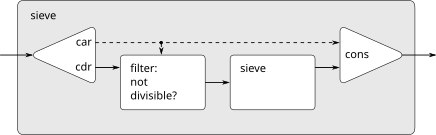
\includegraphics[width=111mm]{assets/figures/chapter_3/figure_3.31.pdf}
\end{imageFigure}

\subsubsection*{Defining streams implicitly}

The \code{integers} and \code{fibs} streams above were defined by specifying
``generating'' procedures that explicitly compute the stream elements one by
one. An alternative way to specify streams is to take advantage of delayed
evaluation to define streams implicitly.  For example, the following expression
defines the stream \code{ones} to be an infinite stream of ones:

\begin{codeBlock}
(define ones (cons-stream 1 ones))
\end{codeBlock}

\noindent
This works much like the definition of a recursive procedure: \code{ones} is a
pair whose \code{car} is 1 and whose \code{cdr} is a promise to evaluate
\code{ones}.  Evaluating the \code{cdr} gives us again a 1 and a promise to
evaluate \code{ones}, and so on.

We can do more interesting things by manipulating streams with operations such
as \code{add\-/streams}, which produces the elementwise sum of two given
streams:\footnote{This uses the generalized version of \code{stream\-/map} from
\link{Exercise 3.50}.}

\begin{codeBlock}
(define (add-streams s1 s2) (stream-map + s1 s2))
\end{codeBlock}

\noindent
Now we can define the integers as follows:

\begin{codeBlock}
(define integers
  (cons-stream 1 (add-streams ones integers)))
\end{codeBlock}

\noindent
This defines \code{integers} to be a stream whose first element is 1 and the
rest of which is the sum of \code{ones} and \code{integers}.  Thus, the second
element of \code{integers} is 1 plus the first element of \code{integers}, or
2; the third element of \code{integers} is 1 plus the second element of
\code{integers}, or 3; and so on.  This definition works because, at any point,
enough of the \code{integers} stream has been generated so that we can feed it
back into the definition to produce the next integer.

We can define the Fibonacci numbers in the same style:

\begin{codeBlock}
(define fibs
  (cons-stream
    0
    (cons-stream 1
                 (add-streams (stream-cdr fibs)
                              fibs))))
\end{codeBlock}

\noindent
This definition says that \code{fibs} is a stream beginning with 0 and 1, such
that the rest of the stream can be generated by adding \code{fibs} to itself
shifted by one place:

\begin{codeBlock}
      1  1  2  3  5  8   13  21  ~\( \dots \)~  =  ~\code{(stream\-/cdr fibs)}~
      0  1  1  2  3  5   8   13  ~\( \dots \)~  =  ~\code{fibs}~
0  1  1  2  3  5  8  13  21  34  ~\( \dots \)~  =  ~\code{fibs}~
\end{codeBlock}

\noindent
\code{scale\-/stream} is another useful procedure in formulating such stream
definitions.  This multiplies each item in a stream by a given constant:

\begin{codeBlock}
(define (scale-stream stream factor)
  (stream-map (lambda (x) (* x factor))
              stream))
\end{codeBlock}

\noindent
For example,

\begin{codeBlock}
(define double (cons-stream 1 (scale-stream double 2)))
\end{codeBlock}

\noindent
produces the stream of powers of 2: 1, 2, 4, 8, 16, 32, \( \dots \).

An alternate definition of the stream of primes can be given by starting with
the integers and filtering them by testing for primality.  We will need the
first prime, 2, to get started:

\begin{codeBlock}
(define primes
  (cons-stream
   2
   (stream-filter prime? (integers-starting-from 3))))
\end{codeBlock}

\noindent
This definition is not so straightforward as it appears, because we will test
whether a number \( n \) is prime by checking whether \( n \) is divisible by a
prime (not by just any integer) less than or equal to \( \sqrt{n} \):

\begin{codeBlock}
(define (prime? n)
  (define (iter ps)
    (cond ((> (square (stream-car ps)) n) true)
          ((divisible? n (stream-car ps)) false)
          (else (iter (stream-cdr ps)))))
  (iter primes))
\end{codeBlock}

\noindent
This is a recursive definition, since \code{primes} is defined in terms of the
\code{prime?} predicate, which itself uses the \code{primes} stream.  The
reason this procedure works is that, at any point, enough of the \code{primes}
stream has been generated to test the primality of the numbers we need to check
next.  That is, for every \( n \) we test for primality, either \( n \) is not
prime (in which case there is a prime already generated that divides it) or
\( n \) is prime (in which case there is a prime already generated---i.e., a
prime less than \( n \)---that is greater than
\( \sqrt{n} \)).\footnote{This last point is very subtle and relies on
the fact that \( p_{n+1} \le p_n^2 \).  (Here, \( p_k \) denotes the
\( k^{\mathrm{th}} \) prime.)  Estimates such as these are very difficult to establish.  The
ancient proof by Euclid that there are an infinite number of primes shows that
\( p_{n+1} \le p_1 p_2 \cdots p_n + 1 \), and no substantially
better result was proved until 1851, when the Russian mathematician
P. L. Chebyshev established that \( p_{n+1} \le 2p_n \) for all \( n \).
This result, originally conjectured in 1845, is known as \newterm{Bertrand's
hypothesis}.  A proof can be found in section 22.3 of \link{Hardy and Wright 1960}.}

\begin{exerciseGroup}
\phantomsection\label{Exercise 3.53}
\exerciseHeading{Exercise 3.53:} Without running the program,
describe the elements of the stream defined by

\begin{codeBlock}
(define s (cons-stream 1 (add-streams s s)))
\end{codeBlock}

\phantomsection\label{Exercise 3.54}
\exerciseHeading{Exercise 3.54:} Define a procedure
\code{mul\-/streams}, analogous to \code{add\-/streams}, that produces the
elementwise product of its two input streams.  Use this together with the
stream of \code{integers} to complete the following definition of the stream
whose \( n^{\mathrm{th}} \) element (counting from 0) is \( n + 1 \) factorial:

\begin{codeBlock}
(define factorials
  (cons-stream 1 (mul-streams ~\(\langle \)~??~\(\rangle \)~ ~\(\langle \)~??~\(\rangle \)~)))
\end{codeBlock}
% \noindent
% \code{(define factorials (cons\-/stream 1 (mul\-/streams}\( \kern0.7ex\langle \)\code{?}\( \rangle \)\( \kern0.7ex\langle \)\code{?}\( \rangle \)\code{)))}

\phantomsection\label{Exercise 3.55}
\exerciseHeading{Exercise 3.55:} Define a procedure
\code{partial\-/sums} that takes as argument a stream \( S \) and returns the
stream whose elements are \( S_0 \), \( S_0 + S_1 \), \( S_0 + S_1 + S_2, \dots \).
For example, \code{(partial\-/sums integers)} should be the
stream 1, 3, 6, 10, 15, \( \dots \).

\phantomsection\label{Exercise 3.56}
\exerciseHeading{Exercise 3.56:} A famous problem, first raised by
R. Hamming, is to enumerate, in ascending order with no repetitions, all
positive integers with no prime factors other than 2, 3, or 5.  One obvious way
to do this is to simply test each integer in turn to see whether it has any
factors other than 2, 3, and 5.  But this is very inefficient, since, as the
integers get larger, fewer and fewer of them fit the requirement.  As an
alternative, let us call the required stream of numbers \code{S} and notice the
following facts about it.

\begin{itemize}
\item
\code{S} begins with 1.

\item
The elements of \code{(scale\-/stream S 2)} are also
elements of \code{S}.

\item
The same is true for \code{(scale\-/stream S 3)}
and \code{(scale\-/stream 5 S)}.

\item
These are all the elements of \code{S}.
\end{itemize}

Now all we have to do is combine elements from these sources.  For this we
define a procedure \code{merge} that combines two ordered streams into one
ordered result stream, eliminating repetitions:

\begin{codeBlock}
(define (merge s1 s2)
  (cond ((stream-null? s1) s2)
        ((stream-null? s2) s1)
        (else
         (let ((s1car (stream-car s1))
               (s2car (stream-car s2)))
           (cond ((< s1car s2car)
                  (cons-stream
                   s1car
                   (merge (stream-cdr s1) s2)))
                 ((> s1car s2car)
                  (cons-stream
                   s2car
                   (merge s1 (stream-cdr s2))))
                 (else
                  (cons-stream
                   s1car
                   (merge (stream-cdr s1)
                          (stream-cdr s2)))))))))
\end{codeBlock}

Then the required stream may be constructed with \code{merge}, as follows:

\begin{codeBlock}
(define S (cons-stream 1 (merge ~\(\langle \)~??~\(\rangle \)~ ~\(\langle \)~??~\(\rangle \)~)))
\end{codeBlock}

Fill in the missing expressions in the places marked \( \langle \)??\( \kern0.08em\rangle \) above.

\phantomsection\label{Exercise 3.57}
\exerciseHeading{Exercise 3.57:} How many additions are performed
when we compute the \( n^{\mathrm{th}} \) Fibonacci number using the definition of
\code{fibs} based on the \code{add\-/streams} procedure?  Show that the number of
additions would be exponentially greater if we had implemented \code{(delay
\( \langle \)\var{exp}\( \rangle \))} simply as \code{(lambda () \( \langle \)\var{exp}\( \rangle \))}, without using the
optimization provided by the \code{memo\-/proc} procedure described in
\link{Section 3.5.1}.\footnote{This exercise shows how call-by-need is closely related
to ordinary memoization as described in \link{Exercise 3.27}.  In that exercise,
we used assignment to explicitly construct a local table.  Our call-by-need
stream optimization effectively constructs such a table automatically, storing
values in the previously forced parts of the stream.}

\phantomsection\label{Exercise 3.58}
\exerciseHeading{Exercise 3.58:} Give an interpretation of the
stream computed by the following procedure:

\begin{codeBlock}
(define (expand num den radix)
  (cons-stream
   (quotient (* num radix) den)
   (expand (remainder (* num radix) den) den radix)))
\end{codeBlock}

(\code{quotient} is a primitive that returns the integer quotient of two
integers.)  What are the successive elements produced by \code{(expand 1 7
10)}?  What is produced by \code{(expand 3 8 10)}?

\phantomsection\label{Exercise 3.59}
\exerciseHeading{Exercise 3.59:} In \link{Section 2.5.3} we saw how
to implement a polynomial arithmetic system representing polynomials as lists
of terms.  In a similar way, we can work with \newterm{power series}, such as

$$
e^x = 1 + x + \displaystyle\frac{x^2}{2} + \displaystyle\frac{x^3}{3 \cdot 2} + \displaystyle\frac{x^4}{4 \cdot 3 \cdot 2} + \dots,
$$


$$
\cos x = 1 - \displaystyle\frac{x^2}{2} + \displaystyle\frac{x^4}{4 \cdot 3 \cdot 2} - \dots,
$$


$$
\sin x = x - \displaystyle\frac{x^3}{3 \cdot 2} + \displaystyle\frac{x^5}{5 \cdot 4 \cdot 3 \cdot 2} - \dots
$$

\noindent
represented as infinite streams.  We will represent the series \( a_0 +
a_1 x + a_2 x^2 + a_3 x^3 + \dots \) as the stream whose
elements are the coefficients \( a_0 \), \( a_1 \), \( a_2 \), \( a_3 \), \( \dots \).

\begin{enumerate}[a.]

\item
The integral of the series \( a_0 + a_1 x + a_2 x^2 + a_3 x^3 + \dots \) is the series

$$ c + a_0 x + \frac{1}{2} a_1 x^2 + \frac{1}{3} a_2 x^3 + \frac{1}{4} a_3 x^4 + \dots, $$

\noindent
where \( c \) is any constant.  Define a procedure \code{integrate\-/series} that
takes as input a stream \( a_0 \), \( a_1 \), \( a_2 \), \( \dots \) representing a power
series and returns the stream \( a_0 \), \( \frac{1}{2}a_1 \), \( \frac{1}{3}a_2 \), \( \dots \) of
coefficients of the non-constant terms of the integral of the series.  (Since
the result has no constant term, it doesn't represent a power series; when we
use \code{integrate\-/series}, we will \code{cons} on the appropriate constant.)

\item
The function \( x \mapsto e^x \) is its own derivative.  This implies that
\( e^x \) and the integral of \( e^x \) are the same series, except for the
constant term, which is \( e^0 = 1 \).  Accordingly, we can generate the series
for \( e^x \) as

\begin{codeBlock}
(define exp-series
  (cons-stream 1 (integrate-series exp-series)))
\end{codeBlock}

Show how to generate the series for sine and cosine, starting from the facts
that the derivative of sine is cosine and the derivative of cosine is the
negative of sine:

\begin{codeBlock}
(define cosine-series (cons-stream 1 ~\(\langle \)~??~\(\rangle \)~))
(define sine-series (cons-stream 0 ~\(\langle \)~??~\(\rangle \)~))
\end{codeBlock}
\end{enumerate}

\phantomsection\label{Exercise 3.60}
\exerciseHeading{Exercise 3.60:} With power series represented as
streams of coefficients as in \link{Exercise 3.59}, adding series is implemented
by \code{add\-/streams}.  Complete the definition of the following procedure for
multiplying series:

\begin{codeBlock}
(define (mul-series s1 s2)
  (cons-stream ~\(\langle \)~??~\(\rangle \)~ (add-streams ~\(\langle \)~??~\(\rangle \)~ ~\(\langle \)~??~\(\rangle \)~)))
\end{codeBlock}

You can test your procedure by verifying that \mbox{\( \sin^2\!x + \cos^2\!x = 1 \)},
using the series from \link{Exercise 3.59}.

\phantomsection\label{Exercise 3.61}
\exerciseHeading{Exercise 3.61:} Let \( S \) be a power series
(\link{Exercise 3.59}) whose constant term is 1.  Suppose we want to find the
power series \( 1 / S \), that is, the series \( X \) such that \( SX = 1 \).
Write \( S = 1 + S_R \) where \( S_R \) is the part of \( S \) after the
constant term.  Then we can solve for \( X \) as follows:

$$
\begin{array}{r@{{}={}}l}
	        S \cdot X 	& 1, \\
	(1 + S_R) \cdot X 	& 1, \\
	  X + S_R \cdot X 	& 1, \\
	            	X 	& 1 - S_R \cdot X.
\end{array}
$$

In other words, \( X \) is the power series whose constant term is 1 and whose
higher-order terms are given by the negative of \( S_R \) times \( X \).  Use
this idea to write a procedure \code{invert\-/unit\-/series} that computes \( 1 / S \)
for a power series \( S \) with constant term 1.  You will need to use
\code{mul\-/series} from \link{Exercise 3.60}.

\phantomsection\label{Exercise 3.62}
\exerciseHeading{Exercise 3.62:} Use the results of \link{Exercise 3.60}
and \link{Exercise 3.61} to define a procedure \code{div\-/series} that
divides two power series.  \code{div\-/series} should work for any two series,
provided that the denominator series begins with a nonzero constant term.  (If
the denominator has a zero constant term, then \code{div\-/series} should signal
an error.)  Show how to use \code{div\-/series} together with the result of
\link{Exercise 3.59} to generate the power series for tangent.
\end{exerciseGroup}

\subsection{Exploiting the Stream Paradigm}
\label{Section 3.5.3}

Streams with delayed evaluation can be a powerful modeling tool, providing many
of the benefits of local state and assignment.  Moreover, they avoid some of
the theoretical tangles that accompany the introduction of assignment into a
programming language.

The stream approach can be illuminating because it allows us to build systems
with different module boundaries than systems organized around assignment to
state variables.  For example, we can think of an entire time series (or
signal) as a focus of interest, rather than the values of the state variables
at individual moments.  This makes it convenient to combine and compare
components of state from different moments.

\subsubsection*{Formulating iterations as stream processes}

In \link{Section 1.2.1}, we introduced iterative processes, which proceed by
updating state variables.  We know now that we can represent state as a
``timeless'' stream of values rather than as a set of variables to be updated.
Let's adopt this perspective in revisiting the square-root procedure from
\link{Section 1.1.7}.  Recall that the idea is to generate a sequence of better
and better guesses for the square root of \( x \) by applying over and over again
the procedure that improves guesses:

\begin{codeBlock}
(define (sqrt-improve guess x)
  (average guess (/ x guess)))
\end{codeBlock}

\noindent
In our original \code{sqrt} procedure, we made these guesses be the successive
values of a state variable. Instead we can generate the infinite stream of
guesses, starting with an initial guess of 1:\footnote{We can't use \code{let}
to bind the local variable \code{guesses}, because the value of \code{guesses}
depends on \code{guesses} itself.  \link{Exercise 3.63} addresses why we want a
local variable here.}

\begin{codeBlock}
(define (sqrt-stream x)
  (define guesses
    (cons-stream
      1.0
      (stream-map (lambda (guess)
                    (sqrt-improve guess x))
                  guesses)))
  guesses)

(display-stream (sqrt-stream 2))
~\textit{1.}~
~\textit{1.5}~
~\textit{1.4166666666666665}~
~\textit{1.4142156862745097}~
~\textit{1.4142135623746899}~
~\( \dots \)~
\end{codeBlock}

\noindent
We can generate more and more terms of the stream to get better and better
guesses.  If we like, we can write a procedure that keeps generating terms
until the answer is good enough.  (See \link{Exercise 3.64}.)

Another iteration that we can treat in the same way is to generate an
approximation to \( \pi \), based upon the alternating series that we saw in
\link{Section 1.3.1}:

$$ \frac{\pi}{4} = 1 - \frac{1}{3} + \frac{1}{5} - frac{1}{7} + \dots. $$

We first generate the stream of summands of the series (the reciprocals of the
odd integers, with alternating signs).  Then we take the stream of sums of more
and more terms (using the \code{partial\-/sums} procedure of
\link{Exercise 3.55}) and scale the result by 4:

\begin{codeBlock}
(define (pi-summands n)
  (cons-stream (/ 1.0 n)
               (stream-map - (pi-summands (+ n 2)))))
(define pi-stream
  (scale-stream (partial-sums (pi-summands 1)) 4))

(display-stream pi-stream)
~\textit{4.}~
~\textit{2.666666666666667}~
~\textit{3.466666666666667}~
~\textit{2.8952380952380956}~
~\textit{3.3396825396825403}~
~\textit{2.9760461760461765}~
~\textit{3.2837384837384844}~
~\textit{3.017071817071818}~
~\( \dots \)~
\end{codeBlock}

\noindent
This gives us a stream of better and better approximations to \( \pi \),
although the approximations converge rather slowly.  Eight terms of the
sequence bound the value of \( \pi \) between 3.284 and 3.017.

So far, our use of the stream of states approach is not much different from
updating state variables.  But streams give us an opportunity to do some
interesting tricks.  For example, we can transform a stream with a
\newterm{sequence accelerator} that converts a sequence of approximations to a
new sequence that converges to the same value as the original, only faster.

One such accelerator, due to the eighteenth-century Swiss mathematician
Leonhard Euler, works well with sequences that are partial sums of alternating
series (series of terms with alternating signs).  In Euler's technique, if
\( S_n \) is the \( n^{\mathrm{th}} \) term of the original sum sequence, then the
accelerated sequence has terms

$$ S_{n+1} - {\frac{(S_{n+1} - S_n)^2}{S_{n-1} - 2S_n + S_{n+1}}}\,. $$

Thus, if the original sequence is represented as a stream of values, the
transformed sequence is given by

\begin{codeBlock}
(define (euler-transform s)
  (let ((s0 (stream-ref s 0))     ~\textrm{; \( S_{n-1} \)}~
        (s1 (stream-ref s 1))     ~\textrm{; \( S_n \)}~
        (s2 (stream-ref s 2)))    ~\textrm{; \( S_{n+1} \)}~
    (cons-stream (- s2 (/ (square (- s2 s1))
                          (+ s0 (* -2 s1) s2)))
                 (euler-transform (stream-cdr s)))))
\end{codeBlock}

\noindent
We can demonstrate Euler acceleration with our sequence of approximations to
\( \pi \):

\begin{codeBlock}
(display-stream (euler-transform pi-stream))
~\textit{3.166666666666667}~
~\textit{3.1333333333333337}~
~\textit{3.1452380952380956}~
~\textit{3.13968253968254}~
~\textit{3.1427128427128435}~
~\textit{3.1408813408813416}~
~\textit{3.142071817071818}~
~\textit{3.1412548236077655}~
~\( \dots \)~
\end{codeBlock}

\noindent
Even better, we can accelerate the accelerated sequence, and recursively
accelerate that, and so on.  Namely, we create a stream of streams (a structure
we'll call a \newterm{tableau}) in which each stream is the transform of the
preceding one:

\begin{codeBlock}
(define (make-tableau transform s)
  (cons-stream s (make-tableau transform (transform s))))
\end{codeBlock}

\noindent
The tableau has the form

\[
\begin{matrix}
s_{00} & s_{01} & s_{02} & s_{03} & s_{04} & \dots \\
       & s_{10} & s_{11} & s_{12} & s_{13} & \dots \\
       &        & s_{20} & s_{21} & s_{22} & \dots \\
       &        &        & \dots  &        & 
\end{matrix}
\]

Finally, we form a sequence by taking the first term in each row of the
tableau:

\begin{codeBlock}
(define (accelerated-sequence transform s)
  (stream-map stream-car (make-tableau transform s)))
\end{codeBlock}

\noindent
We can demonstrate this kind of ``super-acceleration'' of the \( \pi \)
sequence:

\begin{codeBlock}
(display-stream
 (accelerated-sequence euler-transform pi-stream))
~\textit{4.}~
~\textit{3.166666666666667}~
~\textit{3.142105263157895}~
~\textit{3.141599357319005}~
~\textit{3.1415927140337785}~
~\textit{3.1415926539752927}~
~\textit{3.1415926535911765}~
~\textit{3.141592653589778}~
~\( \dots \)~
\end{codeBlock}

\noindent
The result is impressive.  Taking eight terms of the sequence yields the
correct value of \( \pi \) to 14 decimal places.  If we had used only the
original \( \pi \) sequence, we would need to compute on the order of \( 10^{13} \)
terms (i.e., expanding the series far enough so that the individual terms are
less than \( 10^{-13} \)) to get that much accuracy!

We could have implemented these acceleration techniques without using streams.
But the stream formulation is particularly elegant and convenient because the
entire sequence of states is available to us as a data structure that can be
manipulated with a uniform set of operations.

\begin{exerciseGroup}
\phantomsection\label{Exercise 3.63}
\exerciseHeading{Exercise 3.63:} Louis Reasoner asks why the
\code{sqrt\-/stream} procedure was not written in the following more
straightforward way, without the local variable \code{guesses}:

\begin{codeBlock}
(define (sqrt-stream x)
  (cons-stream 1.0 (stream-map
                    (lambda (guess)
                      (sqrt-improve guess x))
                    (sqrt-stream x))))
\end{codeBlock}

Alyssa P. Hacker replies that this version of the procedure is considerably
less efficient because it performs redundant computation.  Explain Alyssa's
answer.  Would the two versions still differ in efficiency if our
implementation of \code{delay} used only \code{(lambda () \( \langle \)\var{exp}\( \rangle \))} without
using the optimization provided by \code{memo\-/proc} (\link{Section 3.5.1})?

\phantomsection\label{Exercise 3.64}
\exerciseHeading{Exercise 3.64:} Write a procedure
\code{stream\-/limit} that takes as arguments a stream and a number (the
tolerance).  It should examine the stream until it finds two successive
elements that differ in absolute value by less than the tolerance, and return
the second of the two elements.  Using this, we could compute square roots up
to a given tolerance by

\begin{codeBlock}
(define (sqrt x tolerance)
  (stream-limit (sqrt-stream x) tolerance))
\end{codeBlock}

\phantomsection\label{Exercise 3.65}
\exerciseHeading{Exercise 3.65:} Use the series

$$ \ln 2 = 1 - \frac{1}{2} + \frac{1}{3} - \frac{1}{4} + \dots $$

\noindent
to compute three sequences of approximations to the natural logarithm of 2, in
the same way we did above for \( \pi \).  How rapidly do these sequences
converge?
\end{exerciseGroup}

\subsubsection*{Infinite streams of pairs}

In \link{Section 2.2.3}, we saw how the sequence paradigm handles traditional
nested loops as processes defined on sequences of pairs.  If we generalize this
technique to infinite streams, then we can write programs that are not easily
represented as loops, because the ``looping'' must range over an infinite set.

For example, suppose we want to generalize the \code{prime\-/sum\-/pairs} procedure
of \link{Section 2.2.3} to produce the stream of pairs of \emph{all} integers
\( (i, j) \) with \( i \le j \) such that \( i + j \) is prime.  If
\code{int\-/pairs} is the sequence of all pairs of integers \( (i, j) \) with
\( i \le j \), then our required stream is simply\footnote{As in
\link{Section 2.2.3}, we represent a pair of integers as a list rather than a Lisp
pair.}

\begin{codeBlock}
(stream-filter
 (lambda (pair) (prime? (+ (car pair) (cadr pair))))
 int-pairs)
\end{codeBlock}

\noindent
Our problem, then, is to produce the stream \code{int\-/pairs}.  More generally,
suppose we have two streams \( S = (S_i) \) and \( T = (T_j) \),
and imagine the infinite rectangular array

\[
\begin{matrix}
(S_0, T_0) & (S_0, T_1) & (S_0, T_2) & \dots \\
(S_1, T_0) & (S_1, T_1) & (S_1, T_2) & \dots \\
(S_2, T_0) & (S_2, T_1) & (S_2, T_2) & \dots \\
\dots      &            &            & 
\end{matrix}
\]

We wish to generate a stream that contains all the pairs in the array that lie
on or above the diagonal, i.e., the pairs

\[
\begin{matrix}
(S_0, T_0) & (S_0, T_1) & (S_0, T_2) & \dots \\
           & (S_1, T_1) & (S_1, T_2) & \dots \\
           &            & (S_2, T_2) & \dots \\
           &            &            & \dots 
\end{matrix}
\]

\noindent
(If we take both \( S \) and \( T \) to be the stream of integers, then this will
be our desired stream \code{int\-/pairs}.)

Call the general stream of pairs \code{(pairs S T)}, and consider it to be
composed of three parts: the pair \( (S_0, T_0) \), the rest of the pairs in
the first row, and the remaining pairs:\footnote{See \link{Exercise 3.68} for
some insight into why we chose this decomposition.}

\[
\begin{array}{c|ccc}
(S_0, T_0) & (S_0, T_1) & (S_0, T_2) & \dots \\
\hline
           & (S_1, T_1) & (S_1, T_2) & \dots \\
           &            & (S_2, T_2) & \dots \\
           &            &            & \dots 
\end{array}
\]

Observe that the third piece in this decomposition (pairs that are not in the
first row) is (recursively) the pairs formed from \code{(stream\-/cdr S)} and
\code{(stream\-/cdr T)}.  Also note that the second piece (the rest of the first
row) is

\begin{codeBlock}
(stream-map (lambda (x) (list (stream-car s) x))
            (stream-cdr t))
\end{codeBlock}

\noindent
Thus we can form our stream of pairs as follows:

\begin{codeBlock}
(define (pairs s t)
  (cons-stream
   (list (stream-car s) (stream-car t))
   (~\(\langle \)~~\var{combine-in-some-way}~~\(\rangle \)~
     (stream-map (lambda (x) (list (stream-car s) x))
                 (stream-cdr t))
     (pairs (stream-cdr s) (stream-cdr t)))))
\end{codeBlock}

\noindent
In order to complete the procedure, we must choose some way to combine the two
inner streams.  One idea is to use the stream analog of the \code{append}
procedure from \link{Section 2.2.1}:

\begin{codeBlock}
(define (stream-append s1 s2)
  (if (stream-null? s1)
      s2
      (cons-stream (stream-car s1)
                   (stream-append (stream-cdr s1)
                                  s2))))
\end{codeBlock}

\noindent
This is unsuitable for infinite streams, however, because it takes all the
elements from the first stream before incorporating the second stream.  In
particular, if we try to generate all pairs of positive integers using

\begin{codeBlock}
(pairs integers integers)
\end{codeBlock}

\noindent
our stream of results will first try to run through all pairs with the first
integer equal to 1, and hence will never produce pairs with any other value of
the first integer.

To handle infinite streams, we need to devise an order of combination that
ensures that every element will eventually be reached if we let our program run
long enough.  An elegant way to accomplish this is with the following
\code{interleave} procedure:\footnote{The precise statement of the required
property on the order of combination is as follows: There should be a function
\( f \) of two arguments such that the pair corresponding to element \( i \) of the
first stream and element \( j \) of the second stream will appear as element
number \( f(i, j) \) of the output stream.  The trick of using
\code{interleave} to accomplish this was shown to us by David Turner, who
employed it in the language KRC (\link{Turner 1981}).}

\begin{codeBlock}
(define (interleave s1 s2)
  (if (stream-null? s1)
      s2
      (cons-stream (stream-car s1)
                   (interleave s2 (stream-cdr s1)))))
\end{codeBlock}

\noindent
Since \code{interleave} takes elements alternately from the two streams, every
element of the second stream will eventually find its way into the interleaved
stream, even if the first stream is infinite.

We can thus generate the required stream of pairs as

\begin{codeBlock}
(define (pairs s t)
  (cons-stream
   (list (stream-car s) (stream-car t))
   (interleave
    (stream-map (lambda (x) (list (stream-car s) x))
                (stream-cdr t))
    (pairs (stream-cdr s) (stream-cdr t)))))
\end{codeBlock}

\begin{exerciseGroup}
\phantomsection\label{Exercise 3.66}
\exerciseHeading{Exercise 3.66:} Examine the stream \code{(pairs
integers integers)}. Can you make any general comments about the order in which
the pairs are placed into the stream? For example, approximately how many pairs precede
the pair (1, 100)?  the pair (99, 100)? the pair (100, 100)? (If you can make
precise mathematical statements here, all the better. But feel free to give
more qualitative answers if you find yourself getting bogged down.)

\phantomsection\label{Exercise 3.67}
\exerciseHeading{Exercise 3.67:} Modify the \code{pairs} procedure
so that \code{(pairs integers integers)} will produce the stream of \emph{all}
pairs of integers \( (i, j) \) (without the condition \( i \le j \)).  Hint:
You will need to mix in an additional stream.

\phantomsection\label{Exercise 3.68}
\exerciseHeading{Exercise 3.68:} Louis Reasoner thinks that
building a stream of pairs from three parts is unnecessarily complicated.
Instead of separating the pair \( (S_0, T_0) \) from the rest of the pairs in
the first row, he proposes to work with the whole first row, as follows:

\begin{codeBlock}
(define (pairs s t)
  (interleave
   (stream-map (lambda (x) (list (stream-car s) x))
               t)
   (pairs (stream-cdr s) (stream-cdr t))))
\end{codeBlock}

Does this work?  Consider what happens if we evaluate \code{(pairs integers
integers)} using Louis's definition of \code{pairs}.

\phantomsection\label{Exercise 3.69}
\exerciseHeading{Exercise 3.69:} Write a procedure \code{triples}
that takes three infinite streams, \( S \), \( T \), and \( U \), and produces the
stream of triples \( (S_i, T_j, U_k) \) such that \( i \le j \le k \).
Use \code{triples} to generate the stream of all Pythagorean
triples of positive integers, i.e., the triples \( (i, j, k) \) such that
\( i \le j \) and \( i^2 + j^2 = k^2 \).

\phantomsection\label{Exercise 3.70}
\exerciseHeading{Exercise 3.70:} It would be nice to be able to
generate streams in which the pairs appear in some useful order, rather than in
the order that results from an \emph{ad hoc} interleaving process.  We can use
a technique similar to the \code{merge} procedure of \link{Exercise 3.56}, if we
define a way to say that one pair of integers is ``less than'' another.  One
way to do this is to define a ``weighting function'' \( W(i, j) \) and
stipulate that \( (i_1, j_1) \) is less than \( (i_2, j_2) \) if
\( W(i_1, j_1) < W(i_2, j_2) \).  Write a procedure
\code{merge\-/weighted} that is like \code{merge}, except that
\code{merge\-/weighted} takes an additional argument \code{weight}, which is a
procedure that computes the weight of a pair, and is used to determine the
order in which elements should appear in the resulting merged
stream.\footnote{We will require that the weighting function be such that the
weight of a pair increases as we move out along a row or down along a column of
the array of pairs.}  Using this, generalize \code{pairs} to a procedure
\code{weighted\-/pairs} that takes two streams, together with a procedure that
computes a weighting function, and generates the stream of pairs, ordered
according to weight.  Use your procedure to generate

\begin{enumerate}[a.]

\item
the stream of all pairs of positive integers \( (i, j) \) with \( i \le j \)
ordered according to the sum \( i + j \),

\item
the stream of all pairs of positive integers \( (i, j) \) with \( i \le j \),
where neither \( i \) nor \( j \) is divisible by 2, 3, or 5, and the pairs are
ordered according to the sum \( 2i + 3\!j + 5i\!j \).

\end{enumerate}

\phantomsection\label{Exercise 3.71}
\exerciseHeading{Exercise 3.71:} Numbers that can be expressed as
the sum of two cubes in more than one way are sometimes called
\newterm{Ramanujan numbers}, in honor of the mathematician Srinivasa
Ramanujan.\footnote{To quote from G. H. Hardy's obituary of Ramanujan (\link{Hardy 1921}):
``It was Mr. Littlewood (I believe) who remarked that `every positive
integer was one of his friends.'  I remember once going to see him when he was
lying ill at Putney.  I had ridden in taxi-cab No. 1729, and remarked that the
number seemed to me a rather dull one, and that I hoped it was not an
unfavorable omen.  `No,' he replied, `it is a very interesting number; it is
the smallest number expressible as the sum of two cubes in two different ways.'
'' The trick of using weighted pairs to generate the Ramanujan numbers was
shown to us by Charles Leiserson.} Ordered streams of pairs provide an elegant
solution to the problem of computing these numbers.  To find a number that can
be written as the sum of two cubes in two different ways, we need only generate
the stream of pairs of integers \( (i, j) \) weighted according to the sum
\( i^3 + j^3 \) (see \link{Exercise 3.70}), then search the stream for two
consecutive pairs with the same weight.  Write a procedure to generate the
Ramanujan numbers.  The first such number is 1,729.  What are the next five?

\phantomsection\label{Exercise 3.72}
\exerciseHeading{Exercise 3.72:} In a similar way to \link{Exercise 3.71}
generate a stream of all numbers that can be written as the sum of two
squares in three different ways (showing how they can be so written).
\end{exerciseGroup}

\subsubsection*{Streams as signals}

We began our discussion of streams by describing them as computational analogs
of the ``signals'' in signal-processing systems.  In fact, we can use streams
to model signal-processing systems in a very direct way, representing the
values of a signal at successive time intervals as consecutive elements of a
stream.  For instance, we can implement an \newterm{integrator} or
\newterm{summer} that, for an input stream \( x = (x_i) \), an initial
value \( C \), and a small increment \( dt \), accumulates the sum

$$ S_i = C + \sum_{j=1}^i x_{\kern-0.07em j} \kern0.1em dt $$

\noindent
and returns the stream of values \( S = (S_i) \).  The following
\code{integral} procedure is reminiscent of the ``implicit style'' definition
of the stream of integers (\link{Section 3.5.2}):

\begin{codeBlock}
(define (integral integrand initial-value dt)
  (define int
    (cons-stream
      initial-value
      (add-streams
        (scale-stream integrand dt)
        int)))
  int)
\end{codeBlock}

\noindent
\link{Figure 3.32} is a picture of a signal-processing system that corresponds
to the \code{integral} procedure.  The input stream is scaled by \( dt \) and
passed through an adder, whose output is passed back through the same adder.
The self-reference in the definition of \code{int} is reflected in the figure
by the feedback loop that connects the output of the adder to one of the
inputs.

% figure 3.32
\begin{imageFigure}
  {The \code{integral} procedure viewed as a signal-processing system.}
  \includegraphics[width=102mm]{assets/figures/chapter_3/figure_3.32.pdf}
\end{imageFigure}

\begin{exerciseGroup}
\phantomsection\label{Exercise 3.73}
\exerciseHeading{Exercise 3.73:} We can model electrical circuits
using streams to represent the values of currents or voltages at a sequence of
times.  For instance, suppose we have an \newterm{RC circuit} consisting of a
resistor of resistance \( R \) and a capacitor of capacitance \( C \) in series.
The voltage response \( v \) of the circuit to an injected current \( i \) is
determined by the formula in \link{Figure 3.33}, whose structure is shown by the
accompanying signal-flow diagram.

% figure 3.33
\begin{imageFigure}
  {An RC circuit and the associated signal-flow diagram.}
  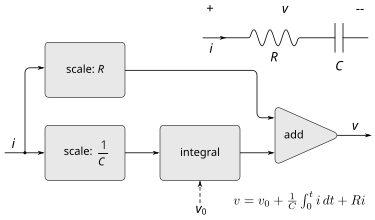
\includegraphics[width=94mm]{assets/figures/chapter_3/figure_3.33.pdf}
\end{imageFigure}

Write a procedure \code{RC} that models this circuit.  \code{RC} should take as
inputs the values of \( R \), \( C \), and \( dt \) and should return a procedure
that takes as inputs a stream representing the current \( i \) and an initial
value for the capacitor voltage \( v_0 \) and produces as output the stream of
voltages \( v \).  For example, you should be able to use \code{RC} to model an
RC circuit with \( R \) = 5 ohms, \( C \) = 1 farad, and a 0.5-second time step by
evaluating \code{(define RC1 (RC 5 1 0.5))}.  This defines \code{RC1} as a
procedure that takes a stream representing the time sequence of currents and an
initial capacitor voltage and produces the output stream of voltages.

\phantomsection\label{Exercise 3.74}
\exerciseHeading{Exercise 3.74:} Alyssa P. Hacker is designing a
system to process signals coming from physical sensors.  One important feature
she wishes to produce is a signal that describes the \newterm{zero crossings}
of the input signal.  That is, the resulting signal should be \( +1 \) whenever the
input signal changes from negative to positive, \( -1 \) whenever the input signal
changes from positive to negative, and 0 otherwise.  (Assume that the sign of a
0 input is positive.)  For example, a typical input signal with its associated
zero-crossing signal would be

\begin{codeBlock}
~\( \dots \)~ 1 2 1.5 1 0.5 -0.1 -2 -3 -2 -0.5 0.2 3 4 ~\( \dots \)~
~\( \dots \)~ 0 0  0  0  0   -1   0  0  0   0   1  0 0 ~\( \dots \)~
\end{codeBlock}

In Alyssa's system, the signal from the sensor is represented as a stream
\code{sense\-/data} and the stream \code{zero\-/crossings} is the corresponding
stream of zero crossings.  Alyssa first writes a procedure
\code{sign\-/change\-/detector} that takes two values as arguments and compares the
signs of the values to produce an appropriate 0, 1, or - 1.  She then
constructs her zero-crossing stream as follows:

\begin{codeBlock}
(define (make-zero-crossings input-stream last-value)
  (cons-stream
   (sign-change-detector
    (stream-car input-stream)
    last-value)
   (make-zero-crossings
    (stream-cdr input-stream)
    (stream-car input-stream))))
(define zero-crossings
  (make-zero-crossings sense-data 0))
\end{codeBlock}

Alyssa's boss, Eva Lu Ator, walks by and suggests that this program is
approximately equivalent to the following one, which uses the generalized
version of \code{stream\-/map} from \link{Exercise 3.50}:

\begin{codeBlock}
(define zero-crossings
  (stream-map sign-change-detector
              sense-data
              ~\(\langle \)~~\var{expression}~~\(\rangle \)~))
\end{codeBlock}

Complete the program by supplying the indicated \( \langle \)\var{expression}\( \rangle \).

\phantomsection\label{Exercise 3.75}
\exerciseHeading{Exercise 3.75:} Unfortunately, Alyssa's
zero-crossing detector in \link{Exercise 3.74} proves to be insufficient,
because the noisy signal from the sensor leads to spurious zero crossings.  Lem
E.  Tweakit, a hardware specialist, suggests that Alyssa smooth the signal to
filter out the noise before extracting the zero crossings.  Alyssa takes his
advice and decides to extract the zero crossings from the signal constructed by
averaging each value of the sense data with the previous value.  She explains
the problem to her assistant, Louis Reasoner, who attempts to implement the
idea, altering Alyssa's program as follows:

\begin{codeBlock}
(define (make-zero-crossings input-stream last-value)
  (let ((avpt (/ (+ (stream-car input-stream)
                    last-value)
                 2)))
    (cons-stream
     (sign-change-detector avpt last-value)
     (make-zero-crossings
      (stream-cdr input-stream) avpt))))
\end{codeBlock}

This does not correctly implement Alyssa's plan.  Find the bug that Louis has
installed and fix it without changing the structure of the program.  (Hint: You
will need to increase the number of arguments to \code{make\-/zero\-/crossings}.)

\phantomsection\label{Exercise 3.76}
\exerciseHeading{Exercise 3.76:} Eva Lu Ator has a criticism of
Louis's approach in \link{Exercise 3.75}.  The program he wrote is not modular,
because it intermixes the operation of smoothing with the zero-crossing
extraction.  For example, the extractor should not have to be changed if Alyssa
finds a better way to condition her input signal.  Help Louis by writing a
procedure \code{smooth} that takes a stream as input and produces a stream in
which each element is the average of two successive input stream elements.
Then use \code{smooth} as a component to implement the zero-crossing detector
in a more modular style.
\end{exerciseGroup}

\subsection{Streams and Delayed Evaluation}
\label{Section 3.5.4}

The \code{integral} procedure at the end of the preceding section shows how we
can use streams to model signal-processing systems that contain feedback loops.
The feedback loop for the adder shown in \link{Figure 3.32} is modeled by the
fact that \code{integral}'s internal stream \code{int} is defined in terms of
itself:

\begin{codeBlock}
(define int
  (cons-stream
   initial-value
   (add-streams (scale-stream integrand dt)
                int)))
\end{codeBlock}

\noindent
The interpreter's ability to deal with such an implicit definition depends on
the \code{delay} that is incorporated into \code{cons\-/stream}.  Without this
\code{delay}, the interpreter could not construct \code{int} before evaluating
both arguments to \code{cons\-/stream}, which would require that \code{int}
already be defined.  In general, \code{delay} is crucial for using streams to
model signal-processing systems that contain loops.  Without \code{delay}, our
models would have to be formulated so that the inputs to any signal-processing
component would be fully evaluated before the output could be produced.  This
would outlaw loops.

% figure 3.34
\begin{imageFigure}
  {An ``analog computer circuit'' that solves the equation \( dy / dt = f(y) \).}
  \includegraphics[width=67mm]{assets/figures/chapter_3/figure_3.34.pdf}
\end{imageFigure}

Unfortunately, stream models of systems with loops may require uses of
\code{delay} beyond the ``hidden'' \code{delay} supplied by \code{cons\-/stream}.
For instance, \link{Figure 3.34} shows a signal-processing system for solving
the differential equation \( dy / dt = f(y) \) where \( f \) is a given
function.  The figure shows a mapping component, which applies \( f \) to its
input signal, linked in a feedback loop to an integrator in a manner very
similar to that of the analog computer circuits that are actually used to solve
such equations.

Assuming we are given an initial value \( y_0 \) for \( y \), we could try to model
this system using the procedure

\begin{codeBlock}
(define (solve f y0 dt)
  (define y (integral dy y0 dt))
  (define dy (stream-map f y))
  y)
\end{codeBlock}

\noindent
This procedure does not work, because in the first line of \code{solve} the
call to \code{integral} requires that the input \code{dy} be defined, which
does not happen until the second line of \code{solve}.

On the other hand, the intent of our definition does make sense, because we
can, in principle, begin to generate the \code{y} stream without knowing
\code{dy}.  Indeed, \code{integral} and many other stream operations have
properties similar to those of \code{cons\-/stream}, in that we can generate part
of the answer given only partial information about the arguments.  For
\code{integral}, the first element of the output stream is the specified
\code{initial\-/value}.  Thus, we can generate the first element of the output
stream without evaluating the integrand \code{dy}.  Once we know the first
element of \code{y}, the \code{stream\-/map} in the second line of \code{solve}
can begin working to generate the first element of \code{dy}, which will
produce the next element of \code{y}, and so on.

To take advantage of this idea, we will redefine \code{integral} to expect the
integrand stream to be a \newterm{delayed argument}.  \code{integral} will
\code{force} the integrand to be evaluated only when it is required to generate
more than the first element of the output stream:

\begin{codeBlock}
(define (integral delayed-integrand initial-value dt)
  (define int
    (cons-stream
     initial-value
     (let ((integrand (force delayed-integrand)))
       (add-streams (scale-stream integrand dt) int))))
  int)
\end{codeBlock}

\noindent
Now we can implement our \code{solve} procedure by delaying the evaluation of
\code{dy} in the definition of \code{y}:\footnote{This procedure is not
guaranteed to work in all Scheme implementations, although for any
implementation there is a simple variation that will work.  The problem has to
do with subtle differences in the ways that Scheme implementations handle
internal definitions.  (See \link{Section 4.1.6}.)}

\begin{codeBlock}
(define (solve f y0 dt)
  (define y (integral (delay dy) y0 dt))
  (define dy (stream-map f y))
  y)
\end{codeBlock}

\noindent
In general, every caller of \code{integral} must now \code{delay} the integrand
argument.  We can demonstrate that the \code{solve} procedure works by
approximating \( e \approx 2.718 \) by computing the value at \( y = 1 \) of the
solution to the differential equation \( dy / dt = y \) with initial
condition \( y(0) = 1 \):

\begin{codeBlock}
(stream-ref (solve (lambda (y) y)
                   1
                   0.001)
            1000)
~\textit{2.716924}~
\end{codeBlock}

\begin{exerciseGroup}
\phantomsection\label{Exercise 3.77}
\exerciseHeading{Exercise 3.77:} The \code{integral} procedure
used above was analogous to the ``implicit'' definition of the infinite stream
of integers in \link{Section 3.5.2}.  Alternatively, we can give a definition of
\code{integral} that is more like \code{integers\-/starting\-/from} (also in
\link{Section 3.5.2}):

\begin{compactCodeBlock}
(define (integral integrand initial-value dt)
  (cons-stream
   initial-value
   (if (stream-null? integrand)
       the-empty-stream
       (integral (stream-cdr integrand)
                 (+ (* dt (stream-car integrand))
                    initial-value)
                 dt))))
\end{compactCodeBlock}

When used in systems with loops, this procedure has the same problem as does
our original version of \code{integral}.  Modify the procedure so that it
expects the \code{integrand} as a delayed argument and hence can be used in the
\code{solve} procedure shown above.

% figure 3.35
\begin{imageFigure}
  {%
    Signal-flow diagram for the solution to a second-order linear differential
    equation.
  }%
  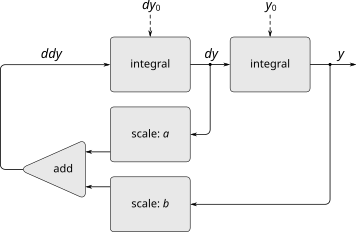
\includegraphics[width=91mm]{assets/figures/chapter_3/figure_3.35a.pdf}
\end{imageFigure}

\phantomsection\label{Exercise 3.78}
\exerciseHeading{Exercise 3.78:} Consider the problem of designing
a signal-processing system to study the homogeneous second-order linear
differential equation

$$ \frac{d^2\!y}{dt^2} - a \frac{dy}{dt} - by = 0. $$

The output stream, modeling \( y \), is generated by a network that contains a
loop. This is because the value of \( d^2\!y / dt^2 \) depends upon the
values of \( y \) and \( dy / dt \) and both of these are determined by
integrating \( d^2\!y / dt^2 \).  The diagram we would like to encode is
shown in \link{Figure 3.35}.  Write a procedure \code{solve\-/2nd} that takes as
arguments the constants \( a \), \( b \), and \( dt \) and the initial values
\( y_0 \) and \( dy_0 \) for \( y \) and \( dy / dt \) and generates the
stream of successive values of \( y \).

\phantomsection\label{Exercise 3.79}
\exerciseHeading{Exercise 3.79:} Generalize the \code{solve\-/2nd}
procedure of \link{Exercise 3.78} so that it can be used to solve general
second-order differential equations \( d^2\!y / dt^2 =
f(dy / dt, y) \).

% figure 3.36
\begin{imageFigure}
  {A series RLC circuit.}
  \includegraphics[width=60mm]{assets/figures/chapter_3/figure_3.36.pdf}
\end{imageFigure}

% figure 3.37
\begin{imageFigure}
  {A signal-flow diagram for the solution to a series RLC circuit.}
  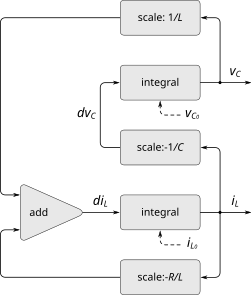
\includegraphics[width=68mm]{assets/figures/chapter_3/figure_3.37a.pdf}
\end{imageFigure}

\phantomsection\label{Exercise 3.80}
\exerciseHeading{Exercise 3.80:} A \newterm{series RLC circuit}
consists of a resistor, a capacitor, and an inductor connected in series, as
shown in \link{Figure 3.36}.  If \( R \), \( L \), and \( C \) are the resistance,
inductance, and capacitance, then the relations between voltage (\( v \)) and
current (\( i \)) for the three components are described by the equations

$$ 	v_R 	= 	i_R R, \qquad\quad
	v_L 	= 	L \frac{di_L}{dt}\,, \qquad\quad
	i_C 	= 	C \frac{dv_C}{dt}\,, $$

and the circuit connections dictate the relations

$$ 	i_R 	= 	i_L = -i_C\,, \qquad\quad
	v_C 	= 	v_L +  v_R\,.  $$

Combining these equations shows that the state of the circuit (summarized by
\( v_C \), the voltage across the capacitor, and \( i_L \), the current in
the inductor) is described by the pair of differential equations

$$  \frac{dv_C}{dt}  =  -\frac{i_L}{C}\,, \qquad\quad
    \frac{di_L}{dt}  =   \frac{1}{L} v_C - \frac{R}{L} i_L\,. $$

The signal-flow diagram representing this system of differential equations is
shown in \link{Figure 3.37}.

Write a procedure \code{RLC} that takes as arguments the parameters \( R \),
\( L \), and \( C \) of the circuit and the time increment \( dt \).  In a manner
similar to that of the \code{RC} procedure of \link{Exercise 3.73}, \code{RLC}
should produce a procedure that takes the initial values of the state
variables, \( v_{C_0} \) and \( i_{L_0} \), and produces a pair (using
\code{cons}) of the streams of states \( v_C \) and \( i_L \).  Using
\code{RLC}, generate the pair of streams that models the behavior of a series
RLC circuit with \( R \) = 1 ohm, \( C \) = 0.2 farad, \( L \) = 1 henry, \( dt \)
= 0.1 second, and initial values \( i_{L_0} \) = 0 amps and \( v_{C_0} \) =
10 volts.
\end{exerciseGroup}

\subsubsection*{Normal-order evaluation}

The examples in this section illustrate how the explicit use of \code{delay}
and \code{force} provides great programming flexibility, but the same examples
also show how this can make our programs more complex.  Our new \code{integral}
procedure, for instance, gives us the power to model systems with loops, but we
must now remember that \code{integral} should be called with a delayed
integrand, and every procedure that uses \code{integral} must be aware of this.
In effect, we have created two classes of procedures: ordinary procedures and
procedures that take delayed arguments.  In general, creating separate classes
of procedures forces us to create separate classes of higher-order procedures
as well.\footnote{This is a small reflection, in Lisp, of the difficulties that
conventional strongly typed languages such as Pascal have in coping with
higher-order procedures.  In such languages, the programmer must specify the
data types of the arguments and the result of each procedure: number, logical
value, sequence, and so on.  Consequently, we could not express an abstraction
such as ``map a given procedure \code{proc} over all the elements in a
sequence'' by a single higher-order procedure such as \code{stream\-/map}.
Rather, we would need a different mapping procedure for each different
combination of argument and result data types that might be specified for a
\code{proc}.  Maintaining a practical notion of ``data type'' in the presence
of higher-order procedures raises many difficult issues.  One way of dealing
with this problem is illustrated by the language ML (\link{Gordon et al. 1979}),
whose ``polymorphic data types'' include templates for
higher-order transformations between data types.  Moreover, data types for most
procedures in ML are never explicitly declared by the programmer.  Instead, ML
includes a \newterm{type-inferencing} mechanism that uses information in the
environment to deduce the data types for newly defined procedures.}

One way to avoid the need for two different classes of procedures is to make
all procedures take delayed arguments.  We could adopt a model of evaluation in
which all arguments to procedures are automatically delayed and arguments are
forced only when they are actually needed (for example, when they are required
by a primitive operation).  This would transform our language to use
normal-order evaluation, which we first described when we introduced the
substitution model for evaluation in \link{Section 1.1.5}.  Converting to
normal-order evaluation provides a uniform and elegant way to simplify the use
of delayed evaluation, and this would be a natural strategy to adopt if we were
concerned only with stream processing.  In \link{Section 4.2}, after we have
studied the evaluator, we will see how to transform our language in just this
way.  Unfortunately, including delays in procedure calls wreaks havoc with our
ability to design programs that depend on the order of events, such as programs
that use assignment, mutate data, or perform input or output.  Even the single
\code{delay} in \code{cons\-/stream} can cause great confusion, as illustrated by
\link{Exercise 3.51} and \link{Exercise 3.52}.  As far as anyone knows,
mutability and delayed evaluation do not mix well in programming languages, and
devising ways to deal with both of these at once is an active area of research.

\subsection{Modularity of Functional Programs and Modularity of Objects}
\label{Section 3.5.5}

As we saw in \link{Section 3.1.2}, one of the major benefits of introducing
assignment is that we can increase the modularity of our systems by
encapsulating, or ``hiding,'' parts of the state of a large system within local
variables.  Stream models can provide an equivalent modularity without the use
of assignment.  As an illustration, we can reimplement the Monte Carlo
estimation of \( \pi \), which we examined in \link{Section 3.1.2}, from a
stream-processing point of view.

The key modularity issue was that we wished to hide the internal state of a
random-number generator from programs that used random numbers.  We began with
a procedure \code{rand\-/update}, whose successive values furnished our supply of
random numbers, and used this to produce a random-number generator:

\begin{codeBlock}
(define rand
  (let ((x random-init))
    (lambda ()
      (set! x (rand-update x))
      x)))
\end{codeBlock}

\noindent
In the stream formulation there is no random-number generator \emph{per se},
just a stream of random numbers produced by successive calls to
\code{rand\-/update}:

\begin{codeBlock}
(define random-numbers
  (cons-stream
   random-init
   (stream-map rand-update random-numbers)))
\end{codeBlock}

\noindent
We use this to construct the stream of outcomes of the Ces\`aro experiment
performed on consecutive pairs in the \code{random\-/numbers} stream:

\begin{codeBlock}
(define cesaro-stream
  (map-successive-pairs
   (lambda (r1 r2) (= (gcd r1 r2) 1))
   random-numbers))
(define (map-successive-pairs f s)
  (cons-stream
   (f (stream-car s) (stream-car (stream-cdr s)))
   (map-successive-pairs f (stream-cdr (stream-cdr s)))))
\end{codeBlock}

\noindent
The \code{cesaro\-/stream} is now fed to a \code{monte\-/carlo} procedure, which
produces a stream of estimates of probabilities.  The results are then
converted into a stream of estimates of \( \pi \).  This version of the program
doesn't need a parameter telling how many trials to perform.  Better estimates
of \( \pi \) (from performing more experiments) are obtained by looking farther
into the \code{pi} stream:

\begin{codeBlock}
(define (monte-carlo experiment-stream passed failed)
  (define (next passed failed)
    (cons-stream
     (/ passed (+ passed failed))
     (monte-carlo
      (stream-cdr experiment-stream) passed failed)))
  (if (stream-car experiment-stream)
      (next (+ passed 1) failed)
      (next passed (+ failed 1))))
(define pi
  (stream-map
   (lambda (p) (sqrt (/ 6 p)))
   (monte-carlo cesaro-stream 0 0)))
\end{codeBlock}

\noindent
There is considerable modularity in this approach, because we still can
formulate a general \code{monte\-/carlo} procedure that can deal with arbitrary
experiments.  Yet there is no assignment or local state.

\begin{exerciseGroup}
\phantomsection\label{Exercise 3.81}
\exerciseHeading{Exercise 3.81:} \link{Exercise 3.6} discussed
generalizing the random-number generator to allow one to reset the
random-number sequence so as to produce repeatable sequences of ``random''
numbers.  Produce a stream formulation of this same generator that operates on
an input stream of requests to \code{generate} a new random number or to
\code{reset} the sequence to a specified value and that produces the desired
stream of random numbers.  Don't use assignment in your solution.

\phantomsection\label{Exercise 3.82}
\exerciseHeading{Exercise 3.82:} Redo \link{Exercise 3.5} on Monte
Carlo integration in terms of streams.  The stream version of
\code{estimate\-/integral} will not have an argument telling how many trials to
perform.  Instead, it will produce a stream of estimates based on successively
more trials.
\end{exerciseGroup}

\subsubsection*{A functional-programming view of time}

Let us now return to the issues of objects and state that were raised at the
beginning of this chapter and examine them in a new light.  We introduced
assignment and mutable objects to provide a mechanism for modular construction
of programs that model systems with state.  We constructed computational
objects with local state variables and used assignment to modify these
variables.  We modeled the temporal behavior of the objects in the world by the
temporal behavior of the corresponding computational objects.

Now we have seen that streams provide an alternative way to model objects with
local state.  We can model a changing quantity, such as the local state of some
object, using a stream that represents the time history of successive states.
In essence, we represent time explicitly, using streams, so that we decouple
time in our simulated world from the sequence of events that take place during
evaluation.  Indeed, because of the presence of \code{delay} there may be
little relation between simulated time in the model and the order of events
during the evaluation.

In order to contrast these two approaches to modeling, let us reconsider the
implementation of a ``withdrawal processor'' that monitors the balance in a
bank account.  In \link{Section 3.1.3} we implemented a simplified version of
such a processor:

\begin{codeBlock}
(define (make-simplified-withdraw balance)
  (lambda (amount)
    (set! balance (- balance amount))
    balance))
\end{codeBlock}

\noindent
Calls to \code{make\-/simplified\-/withdraw} produce computational objects, each
with a local state variable \code{balance} that is decremented by successive
calls to the object.  The object takes an \code{amount} as an argument and
returns the new balance.  We can imagine the user of a bank account typing a
sequence of inputs to such an object and observing the sequence of returned
values shown on a display screen.

Alternatively, we can model a withdrawal processor as a procedure that takes as
input a balance and a stream of amounts to withdraw and produces the stream of
successive balances in the account:

\begin{codeBlock}
(define (stream-withdraw balance amount-stream)
  (cons-stream
   balance
   (stream-withdraw (- balance
                       (stream-car amount-stream))
                    (stream-cdr amount-stream))))
\end{codeBlock}

\noindent
\code{stream\-/withdraw} implements a well-defined mathematical function whose
output is fully determined by its input.  Suppose, however, that the input
\code{amount\-/stream} is the stream of successive values typed by the user and
that the resulting stream of balances is displayed.  Then, from the perspective
of the user who is typing values and watching results, the stream process has
the same behavior as the object created by \code{make\-/simplified\-/withdraw}.
However, with the stream version, there is no assignment, no local state
variable, and consequently none of the theoretical difficulties that we
encountered in \link{Section 3.1.3}.  Yet the system has state!

This is really remarkable.  Even though \code{stream\-/withdraw} implements a
well-defined mathematical function whose behavior does not change, the user's
perception here is one of interacting with a system that has a changing state.
One way to resolve this paradox is to realize that it is the user's temporal
existence that imposes state on the system.  If the user could step back from
the interaction and think in terms of streams of balances rather than
individual transactions, the system would appear stateless.\footnote{Similarly
in physics, when we observe a moving particle, we say that the position (state)
of the particle is changing.  However, from the perspective of the particle's
world line in space-time there is no change involved.}

From the point of view of one part of a complex process, the other parts appear
to change with time.  They have hidden time-varying local state.  If we wish to
write programs that model this kind of natural decomposition in our world (as
we see it from our viewpoint as a part of that world) with structures in our
computer, we make computational objects that are not functional---they must
change with time.  We model state with local state variables, and we model the
changes of state with assignments to those variables.  By doing this we make
the time of execution of a computation model time in the world that we are part
of, and thus we get ``objects'' in our computer.

Modeling with objects is powerful and intuitive, largely because this matches
the perception of interacting with a world of which we are part.  However, as
we've seen repeatedly throughout this chapter, these models raise thorny
problems of constraining the order of events and of synchronizing multiple
processes.  The possibility of avoiding these problems has stimulated the
development of \newterm{functional programming languages}, which do not include
any provision for assignment or mutable data.  In such a language, all
procedures implement well-defined mathematical functions of their arguments,
whose behavior does not change.  The functional approach is extremely
attractive for dealing with concurrent systems.\footnote{John Backus, the
inventor of Fortran, gave high visibility to functional programming when he was
awarded the \acronym{ACM} Turing award in 1978.  His acceptance speech
(\link{Backus 1978}) strongly advocated the functional approach.  A good overview of
functional programming is given in \link{Henderson 1980} and in
\link{Darlington et al. 1982}.}

On the other hand, if we look closely, we can see time-related problems
creeping into functional models as well.  One particularly troublesome area
arises when we wish to design interactive systems, especially ones that model
interactions between independent entities.  For instance, consider once more
the implementation of a banking system that permits joint bank accounts.  In a
conventional system using assignment and objects, we would model the fact that
Peter and Paul share an account by having both Peter and Paul send their
transaction requests to the same bank-account object, as we saw in
\link{Section 3.1.3}.  From the stream point of view, where there are no ``objects''
\emph{per se}, we have already indicated that a bank account can be modeled as
a process that operates on a stream of transaction requests to produce a stream
of responses.  Accordingly, we could model the fact that Peter and Paul have a
joint bank account by merging Peter's stream of transaction requests with
Paul's stream of requests and feeding the result to the bank-account stream
process, as shown in \link{Figure 3.38}.

% figure 3.38
\begin{imageFigure}
  {A joint bank account, modeled by merging two streams of transaction requests.}
  \includegraphics[width=88mm]{assets/figures/chapter_3/figure_3.38.pdf}
\end{imageFigure}

The trouble with this formulation is in the notion of \newterm{merge}.  It will
not do to merge the two streams by simply taking alternately one request from
Peter and one request from Paul. Suppose Paul accesses the account only very
rarely.  We could hardly force Peter to wait for Paul to access the account
before he could issue a second transaction.  However such a merge is
implemented, it must interleave the two transaction streams in some way that is
constrained by ``real time'' as perceived by Peter and Paul, in the sense that,
if Peter and Paul meet, they can agree that certain transactions were processed
before the meeting, and other transactions were processed after the
meeting.\footnote{Observe that, for any two streams, there is in general more
than one acceptable order of interleaving.  Thus, technically, ``merge'' is a
relation rather than a function---the answer is not a deterministic function of
the inputs.  We already mentioned (\link{Footnote 39}) that nondeterminism is
essential when dealing with concurrency.  The merge relation illustrates the
same essential nondeterminism, from the functional perspective.  In
\link{Section 4.3}, we will look at nondeterminism from yet another point of view.} This
is precisely the same constraint that we had to deal with in
\link{Section 3.4.1}, where we found the need to introduce explicit synchronization to
ensure a ``correct'' order of events in concurrent processing of objects with
state.  Thus, in an attempt to support the functional style, the need to merge
inputs from different agents reintroduces the same problems that the functional
style was meant to eliminate.

\ifnum\paperType=0 %
  \newpage
\fi

We began this chapter with the goal of building computational models whose
structure matches our perception of the real world we are trying to model.  We
can model the world as a collection of separate, time-bound, interacting
objects with state, or we can model the world as a single, timeless, stateless
unity.  Each view has powerful advantages, but neither view alone is completely
satisfactory.  A grand unification has yet to emerge.\footnote{The object model
approximates the world by dividing it into separate pieces.  The functional
model does not modularize along object boundaries.  The object model is useful
when the unshared state of the ``objects'' is much larger than the state that
they share.  An example of a place where the object viewpoint fails is quantum
mechanics, where thinking of things as individual particles leads to paradoxes
and confusions.  Unifying the object view with the functional view may have
little to do with programming, but rather with fundamental epistemological
issues.}

  \chapter{Metalinguistic Abstraction}
\label{Chapter 4}

\chapterQuote{%
    \( \dots \) It's in words that the magic is --- Abracadabra, Open Sesame,
    and the rest --- but the magic words in one story aren't magical in the
    next. The real magic is to understand which words work, and when, and for
    what; the trick is to learn the trick.

    \( \dots \) And those words are made from the letters of our alphabet: a
    couple-dozen squiggles we can draw with the pen.  This is the key!  And the
    treasure, too, if we can only get our hands on it!  It's as if --- as if
    the key to the treasure \emph{is} the treasure!
  }
  {John Barth}
  {Chimera}
  {}

\noindent
\lettrine{I}{n our study of program design}, we have seen that expert programmers control
the complexity of their designs with the same general techniques used by
designers of all complex systems.  They combine primitive elements to form
compound objects, they abstract compound objects to form higher-level building
blocks, and they preserve modularity by adopting appropriate large-scale views
of system structure.  In illustrating these techniques, we have used Lisp as a
language for describing processes and for constructing computational data
objects and processes to model complex phenomena in the real world.  However,
as we confront increasingly complex problems, we will find that Lisp, or indeed
any fixed programming language, is not sufficient for our needs.  We must
constantly turn to new languages in order to express our ideas more
effectively.  Establishing new languages is a powerful strategy for controlling
complexity in engineering design; we can often enhance our ability to deal with
a complex problem by adopting a new language that enables us to describe (and
hence to think about) the problem in a different way, using primitives, means
of combination, and means of abstraction that are particularly well suited to
the problem at hand.\footnote{The same idea is pervasive throughout all of
engineering.  For example, electrical engineers use many different languages
for describing circuits.  Two of these are the language of electrical
\newterm{networks} and the language of electrical \newterm{systems}.  The
network language emphasizes the physical modeling of devices in terms of
discrete electrical elements.  The primitive objects of the network language
are primitive electrical components such as resistors, capacitors, inductors,
and transistors, which are characterized in terms of physical variables called
voltage and current.  When describing circuits in the network language, the
engineer is concerned with the physical characteristics of a design.  In
contrast, the primitive objects of the system language are signal-processing
modules such as filters and amplifiers.  Only the functional behavior of the
modules is relevant, and signals are manipulated without concern for their
physical realization as voltages and currents.  The system language is erected
on the network language, in the sense that the elements of signal-processing
systems are constructed from electrical networks.  Here, however, the concerns
are with the large-scale organization of electrical devices to solve a given
application problem; the physical feasibility of the parts is assumed.  This
layered collection of languages is another example of the stratified design
technique illustrated by the picture language of \link{Section 2.2.4}.}

Programming is endowed with a multitude of languages.  There are physical
languages, such as the machine languages for particular computers.  These
languages are concerned with the representation of data and control in terms of
individual bits of storage and primitive machine instructions.  The
machine-language programmer is concerned with using the given hardware to erect
systems and utilities for the efficient implementation of resource-limited
computations.  High-level languages, erected on a machine-language substrate,
hide concerns about the representation of data as collections of bits and the
representation of programs as sequences of primitive instructions.  These
languages have means of combination and abstraction, such as procedure
definition, that are appropriate to the larger-scale organization of systems.

\newterm{Metalinguistic abstraction}---establishing new languages---plays an
important role in all branches of engineering design.  It is particularly
important to computer programming, because in programming not only can we
formulate new languages but we can also implement these languages by
constructing evaluators.  An \newterm{evaluator} (or \newterm{interpreter}) for
a programming language is a procedure that, when applied to an expression of
the language, performs the actions required to evaluate that expression.

It is no exaggeration to regard this as the most fundamental idea in
programming:

\begin{niceQuote}
The evaluator, which determines the meaning of expressions in a programming
language, is just another program.
\end{niceQuote}

\noindent
To appreciate this point is to change our images of ourselves as programmers.
We come to see ourselves as designers of languages, rather than only users of
languages designed by others.

In fact, we can regard almost any program as the evaluator for some language.
For instance, the polynomial manipulation system of \link{Section 2.5.3}
embodies the rules of polynomial arithmetic and implements them in terms of
operations on list-structured data.  If we augment this system with procedures
to read and print polynomial expressions, we have the core of a special-purpose
language for dealing with problems in symbolic mathematics.  The digital-logic
simulator of \link{Section 3.3.4} and the constraint propagator of
\link{Section 3.3.5} are legitimate languages in their own right, each with its own
primitives, means of combination, and means of abstraction.  Seen from this
perspective, the technology for coping with large-scale computer systems merges
with the technology for building new computer languages, and computer science
itself becomes no more (and no less) than the discipline of constructing
appropriate descriptive languages.

We now embark on a tour of the technology by which languages are established in
terms of other languages.  In this chapter we shall use Lisp as a base,
implementing evaluators as Lisp procedures.  Lisp is particularly well suited
to this task, because of its ability to represent and manipulate symbolic
expressions.  We will take the first step in understanding how languages are
implemented by building an evaluator for Lisp itself.  The language implemented
by our evaluator will be a subset of the Scheme dialect of Lisp that we use in
this book.  Although the evaluator described in this chapter is written for a
particular dialect of Lisp, it contains the essential structure of an evaluator
for any expression-oriented language designed for writing programs for a
sequential machine.  (In fact, most language processors contain, deep within
them, a little ``Lisp'' evaluator.)  The evaluator has been simplified for the
purposes of illustration and discussion, and some features have been left out
that would be important to include in a production-quality Lisp system.
Nevertheless, this simple evaluator is adequate to execute most of the programs
in this book.\footnote{The most important features that our evaluator leaves
out are mechanisms for handling errors and supporting debugging.  For a more
extensive discussion of evaluators, see \link{Friedman et al. 1992}, which
gives an exposition of programming languages that proceeds via a sequence of
evaluators written in Scheme.}

An important advantage of making the evaluator accessible as a Lisp program is
that we can implement alternative evaluation rules by describing these as
modifications to the evaluator program.  One place where we can use this power
to good effect is to gain extra control over the ways in which computational
models embody the notion of time, which was so central to the discussion in
\link{Chapter 3}.  There, we mitigated some of the complexities of state and
assignment by using streams to decouple the representation of time in the world
from time in the computer.  Our stream programs, however, were sometimes
cumbersome, because they were constrained by the applicative-order evaluation
of Scheme.  In \link{Section 4.2}, we'll change the underlying language to
provide for a more elegant approach, by modifying the evaluator to provide for
\newterm{normal-order evaluation}.

\link{Section 4.3} implements a more ambitious linguistic change, whereby
expressions have many values, rather than just a single value.  In this
language of \newterm{nondeterministic computing}, it is natural to express
processes that generate all possible values for expressions and then search for
those values that satisfy certain constraints.  In terms of models of
computation and time, this is like having time branch into a set of ``possible
futures'' and then searching for appropriate time lines.  With our
nondeterministic evaluator, keeping track of multiple values and performing
searches are handled automatically by the underlying mechanism of the language.

In \link{Section 4.4} we implement a \newterm{logic-programming} language in
which knowledge is expressed in terms of relations, rather than in terms of
computations with inputs and outputs.  Even though this makes the language
drastically different from Lisp, or indeed from any conventional language, we
will see that the logic-programming evaluator shares the essential structure of
the Lisp evaluator.



\section{The Metacircular Evaluator}
\label{Section 4.1}

Our evaluator for Lisp will be implemented as a Lisp program.  It may seem
circular to think about evaluating Lisp programs using an evaluator that is
itself implemented in Lisp.  However, evaluation is a process, so it is
appropriate to describe the evaluation process using Lisp, which, after all, is
our tool for describing processes.\footnote{Even so, there will remain
important aspects of the evaluation process that are not elucidated by our
evaluator.  The most important of these are the detailed mechanisms by which
procedures call other procedures and return values to their callers.  We will
address these issues in \link{Chapter 5}, where we take a closer look at the
evaluation process by implementing the evaluator as a simple register machine.}
An evaluator that is written in the same language that it evaluates is said to
be \newterm{metacircular}.

The metacircular evaluator is essentially a Scheme formulation of the
environment model of evaluation described in \link{Section 3.2}.  Recall that
the model has two basic parts:

\begin{enumerate}

\item
To evaluate a combination (a compound expression other than a special form),
evaluate the subexpressions and then apply the value of the operator
subexpression to the values of the operand subexpressions.

\item
To apply a compound procedure to a set of arguments, evaluate the body of the
procedure in a new environment.  To construct this environment, extend the
environment part of the procedure object by a frame in which the formal
parameters of the procedure are bound to the arguments to which the procedure
is applied.

\end{enumerate}

\noindent
These two rules describe the essence of the evaluation process, a basic cycle
in which expressions to be evaluated in environments are reduced to procedures
to be applied to arguments, which in turn are reduced to new expressions to be
evaluated in new environments, and so on, until we get down to symbols, whose
values are looked up in the environment, and to primitive procedures, which are
applied directly (see \link{Figure 4.1}).\footnote{If we grant ourselves the
ability to apply primitives, then what remains for us to implement in the
evaluator?  The job of the evaluator is not to specify the primitives of the
language, but rather to provide the connective tissue---the means of
combination and the means of abstraction---that binds a collection of
primitives to form a language. Specifically:

\( \bullet \) The evaluator enables us to deal with nested expressions.  For example,
although simply applying primitives would suffice for evaluating the expression
\code{(+ 1 6)}, it is not adequate for handling \code{(+ 1 (* 2 3))}.  As far
as the primitive procedure \code{+} is concerned, its arguments must be
numbers, and it would choke if we passed it the expression \code{(* 2 3)} as an
argument.  One important role of the evaluator is to choreograph procedure
composition so that \code{(* 2 3)} is reduced to 6 before being passed as an
argument to \code{+}.

\( \bullet \) The evaluator allows us to use variables.  For example, the primitive procedure
for addition has no way to deal with expressions such as \code{(+ x 1)}.  We
need an evaluator to keep track of variables and obtain their values before
invoking the primitive procedures.

\( \bullet \) The evaluator allows us to define compound procedures.  This involves keeping
track of procedure definitions, knowing how to use these definitions in
evaluating expressions, and providing a mechanism that enables procedures to
accept arguments.

\( \bullet \) The evaluator provides the special forms, which must be evaluated differently
from procedure calls.}
This evaluation cycle will be embodied by the interplay between the two
critical procedures in the evaluator, \code{eval} and \code{apply}, which are
described in \link{Section 4.1.1} (see \link{Figure 4.1}).

The implementation of the evaluator will depend upon procedures that define the
\newterm{syntax} of the expressions to be evaluated.  We will use data
abstraction to make the evaluator independent of the representation of the
language.  For example, rather than committing to a choice that an assignment
is to be represented by a list beginning with the symbol \code{set!} we use an
abstract predicate \code{assignment?} to test for an assignment, and we use
abstract selectors \code{assignment\-/variable} and \code{assignment\-/value} to
access the parts of an assignment.  Implementation of expressions will be
described in detail in \link{Section 4.1.2}.  There are also operations,
described in \link{Section 4.1.3}, that specify the representation of procedures
and environments.  For example, \code{make\-/procedure} constructs compound
procedures, \code{lookup\-/variable\-/value} accesses the values of variables, and
\code{apply\-/primitive\-/procedure} applies a primitive procedure to a given list
of arguments.

% figure 4.1
\begin{imageFigure}
  {%
    The \code{eval}-\code{apply} cycle exposes the essence of a computer
    language.
  }%
  
\includegraphics[width=100mm]{assets/figures/chapter_4/figure_4.1.pdf}
\end{imageFigure}

\subsection{The Core of the Evaluator}
\label{Section 4.1.1}

The evaluation process can be described as the interplay between two
procedures: \code{eval} and \code{apply}.

\subsubsection*{Eval}

\code{eval} takes as arguments an expression and an environment.  It classifies
the expression and directs its evaluation.  \code{eval} is structured as a case
analysis of the syntactic type of the expression to be evaluated.  In order to
keep the procedure general, we express the determination of the type of an
expression abstractly, making no commitment to any particular representation
for the various types of expressions.  Each type of expression has a predicate
that tests for it and an abstract means for selecting its parts.  This
\newterm{abstract syntax} makes it easy to see how we can change the syntax of
the language by using the same evaluator, but with a different collection of
syntax procedures.

\bigskip
\noindent
\textbf{Primitive expressions}

\begin{itemize}

\item
For self-evaluating expressions, such as numbers, \code{eval} returns the
expression itself.

\item
\code{eval} must look up variables in the environment to find their values.

\end{itemize}

\noindent
\textbf{Special forms}

\begin{itemize}

\item
For quoted expressions, \code{eval} returns the expression that was quoted.

\item
An assignment to (or a definition of) a variable must recursively call
\code{eval} to compute the new value to be associated with the variable.  The
environment must be modified to change (or create) the binding of the variable.

\item
An \code{if} expression requires special processing of its parts, so as to
evaluate the consequent if the predicate is true, and otherwise to evaluate the
alternative.

\item
A \code{lambda} expression must be transformed into an applicable procedure by
packaging together the parameters and body specified by the \code{lambda}
expression with the environment of the evaluation.

\item
A \code{begin} expression requires evaluating its sequence of expressions in
the order in which they appear.

\item
A case analysis (\code{cond}) is transformed into a nest of \code{if}
expressions and then evaluated.

\end{itemize}

\noindent
\textbf{Combinations}

\begin{itemize}

\item
For a procedure application, \code{eval} must recursively evaluate the operator
part and the operands of the combination.  The resulting procedure and
arguments are passed to \code{apply}, which handles the actual procedure
application.

\end{itemize}

\noindent
Here is the definition of \code{eval}:

\begin{codeBlock}
(define (eval exp env)
  (cond ((self-evaluating? exp) exp)
        ((variable? exp) (lookup-variable-value exp
                                                env))
        ((quoted? exp) (text-of-quotation exp))
        ((assignment? exp) (eval-assignment exp env))
        ((definition? exp) (eval-definition exp env))
        ((if? exp) (eval-if exp env))
        ((lambda? exp)
          (make-procedure (lambda-parameters exp)
                          (lambda-body exp)
                          env))
        ((begin? exp)
         (eval-sequence (begin-actions exp) env))
        ((cond? exp) (eval (cond->if exp) env))
        ((application? exp)
         (apply (eval (operator exp) env)
                (list-of-values (operands exp) env)))
        (else
         (error "Unknown expression type: EVAL" exp))))
\end{codeBlock}

\noindent
For clarity, \code{eval} has been implemented as a case analysis using
\code{cond}.  The disadvantage of this is that our procedure handles only a few
distinguishable types of expressions, and no new ones can be defined without
editing the definition of \code{eval}.  In most Lisp implementations,
dispatching on the type of an expression is done in a data-directed style.
This allows a user to add new types of expressions that \code{eval} can
distinguish, without modifying the definition of \code{eval} itself.  (See
\link{Exercise 4.3}.)

\subsubsection*{Apply}

\code{apply} takes two arguments, a procedure and a list of arguments to which
the procedure should be applied.  \code{apply} classifies procedures into two
kinds: It calls \code{apply\-/primitive\-/procedure} to apply primitives; it
applies compound procedures by sequentially evaluating the expressions that
make up the body of the procedure.  The environment for the evaluation of the
body of a compound procedure is constructed by extending the base environment
carried by the procedure to include a frame that binds the parameters of the
procedure to the arguments to which the procedure is to be applied.  Here is
the definition of \code{apply}:

\begin{codeBlock}
(define (apply procedure arguments)
  (cond ((primitive-procedure? procedure)
         (apply-primitive-procedure procedure
                                    arguments))
        ((compound-procedure? procedure)
         (eval-sequence
           (procedure-body procedure)
           (extend-environment
             (procedure-parameters procedure)
             arguments
             (procedure-environment procedure))))
        (else
         (error
          "Unknown procedure type: APPLY" procedure))))
\end{codeBlock}

\subsubsection*{Procedure arguments}

When \code{eval} processes a procedure application, it uses
\code{list\-/of\-/values} to produce the list of arguments to which the procedure
is to be applied. \code{list\-/of\-/values} takes as an argument the operands of
the combination.  It evaluates each operand and returns a list of the
corresponding values:\footnote{We could have simplified the \code{application?}
clause in \code{eval} by using \code{map} (and stipulating that \code{operands}
returns a list) rather than writing an explicit \code{list\-/of\-/values}
procedure.  We chose not to use \code{map} here to emphasize the fact that the
evaluator can be implemented without any use of higher-order procedures (and
thus could be written in a language that doesn't have higher-order procedures),
even though the language that it supports will include higher-order
procedures.}

\begin{codeBlock}
(define (list-of-values exps env)
  (if (no-operands? exps)
      '()
      (cons (eval (first-operand exps) env)
            (list-of-values (rest-operands exps) env))))
\end{codeBlock}

\subsubsection*{Conditionals}

\code{eval\-/if} evaluates the predicate part of an \code{if} expression in the
given environment.  If the result is true, \code{eval\-/if} evaluates the
consequent, otherwise it evaluates the alternative:

\begin{codeBlock}
(define (eval-if exp env)
  (if (true? (eval (if-predicate exp) env))
      (eval (if-consequent exp) env)
      (eval (if-alternative exp) env)))
\end{codeBlock}

\noindent
The use of \code{true?} in \code{eval\-/if} highlights the issue of the
connection between an implemented language and an implementation language.  The
\code{if\-/predicate} is evaluated in the language being implemented and thus
yields a value in that language.  The interpreter predicate \code{true?}
translates that value into a value that can be tested by the \code{if} in the
implementation language: The metacircular representation of truth might not be
the same as that of the underlying Scheme.\footnote{In this case, the language
being implemented and the implementation language are the same.  Contemplation
of the meaning of \code{true?} here yields expansion of consciousness without
the abuse of substance.}

\subsubsection*{Sequences}

\code{eval\-/sequence} is used by \code{apply} to evaluate the sequence of
expressions in a procedure body and by \code{eval} to evaluate the sequence of
expressions in a \code{begin} expression.  It takes as arguments a sequence of
expressions and an environment, and evaluates the expressions in the order in
which they occur.  The value returned is the value of the final expression.

\begin{codeBlock}
(define (eval-sequence exps env)
  (cond ((last-exp? exps)
         (eval (first-exp exps) env))
        (else
         (eval (first-exp exps) env)
         (eval-sequence (rest-exps exps) env))))
\end{codeBlock}

\subsubsection*{Assignments and definitions}

The following procedure handles assignments to variables.  It calls \code{eval}
to find the value to be assigned and transmits the variable and the resulting
value to \code{set\-/variable\-/value!} to be installed in the designated
environment.

\begin{codeBlock}
(define (eval-assignment exp env)
  (set-variable-value! (assignment-variable exp)
                       (eval (assignment-value exp)
                             env)
                       env)
  'ok)
\end{codeBlock}

\noindent
Definitions of variables are handled in a similar manner.\footnote{This
implementation of \code{define} ignores a subtle issue in the handling of
internal definitions, although it works correctly in most cases.  We will see
what the problem is and how to solve it in \link{Section 4.1.6}.}

\begin{codeBlock}
(define (eval-definition exp env)
  (define-variable! (definition-variable exp)
                    (eval (definition-value exp) env)
                    env)
  'ok)
\end{codeBlock}

\noindent
We have chosen here to return the symbol \code{ok} as the value of an
assignment or a definition.\footnote{As we said when we introduced
\code{define} and \code{set!}, these values are implementation-dependent in
Scheme---that is, the implementor can choose what value to return.}

\begin{exerciseGroup}
\exerciseHeading{\phantomsection\label{Exercise 4.1}Exercise 4.1:} Notice that we cannot tell whether
the metacircular evaluator evaluates operands from left to right or from right
to left.  Its evaluation order is inherited from the underlying Lisp: If the
arguments to \code{cons} in \code{list\-/of\-/values} are evaluated from left to
right, then \code{list\-/of\-/values} will evaluate operands from left to right;
and if the arguments to \code{cons} are evaluated from right to left, then
\code{list\-/of\-/values} will evaluate operands from right to left.

Write a version of \code{list\-/of\-/values} that evaluates operands from left to
right regardless of the order of evaluation in the underlying Lisp.  Also write
a version of \code{list\-/of\-/values} that evaluates operands from right to left.
\end{exerciseGroup}

\subsection{Representing Expressions}
\label{Section 4.1.2}

The evaluator is reminiscent of the symbolic differentiation program discussed
in \link{Section 2.3.2}.  Both programs operate on symbolic expressions.  In
both programs, the result of operating on a compound expression is determined
by operating recursively on the pieces of the expression and combining the
results in a way that depends on the type of the expression.  In both programs
we used data abstraction to decouple the general rules of operation from the
details of how expressions are represented.  In the differentiation program
this meant that the same differentiation procedure could deal with algebraic
expressions in prefix form, in infix form, or in some other form.  For the
evaluator, this means that the syntax of the language being evaluated is
determined solely by the procedures that classify and extract pieces of
expressions.

Here is the specification of the syntax of our language:

\begin{itemize}

\item
The only self-evaluating items are numbers and strings:

\begin{codeBlock}
(define (self-evaluating? exp)
  (cond ((number? exp) true)
        ((string? exp) true)
        (else false)))
\end{codeBlock}

\item
Variables are represented by symbols:

\begin{codeBlock}
(define (variable? exp) (symbol? exp))
\end{codeBlock}

\item
Quotations have the form \code{(quote \( \langle \)\var{text\-/of\-/quotation}\( \rangle \))}:\footnote{As
mentioned in \link{Section 2.3.1}, the evaluator sees a quoted expression as a
list beginning with \code{quote}, even if the expression is typed with the
quotation mark.  For example, the expression \code{'a} would be seen by the
evaluator as \code{(quote a)}.  See \link{Exercise 2.55}.}

\begin{codeBlock}
(define (quoted? exp) (tagged-list? exp 'quote))
(define (text-of-quotation exp) (cadr exp))
\end{codeBlock}

\code{quoted?} is defined in terms of the procedure \code{tagged\-/list?}, which
identifies lists beginning with a designated symbol:

\begin{codeBlock}
(define (tagged-list? exp tag)
  (if (pair? exp)
      (eq? (car exp) tag)
      false))
\end{codeBlock}

\item
Assignments have the form \code{(set! \( \langle \)\var{var}\( \rangle \)
\( \langle \)\var{value}\( \rangle \))}:

\begin{codeBlock}
(define (assignment? exp) (tagged-list? exp 'set!))
(define (assignment-variable exp) (cadr exp))
(define (assignment-value exp) (caddr exp))
\end{codeBlock}

\item
Definitions have the form

\begin{codeBlock}
(define ~\(\langle \)~~\var{var}~~\(\rangle \)~ ~\(\langle \)~~\var{value}~~\(\rangle \)~)
\end{codeBlock}

\noindent
or the form

\begin{codeBlock}
(define (~\(\langle \)~~\var{var}~~\(\rangle \)~ ~\(\langle \)~~\var{parameter}~~\(_{\mono{1}}\rangle \)~ ~\( \dots \)~ ~\(\langle \)~~\var{parameter}~~\(_{\monoItalic{n}}\rangle \)~)
  ~\(\langle \)~~\var{body}~~\(\rangle \)~)
\end{codeBlock}

The latter form (standard procedure definition) is syntactic sugar for

\begin{codeBlock}
(define ~\(\langle \)~~\var{var}~~\(\rangle \)~
  (lambda (~\(\langle \)~~\var{parameter}~~\(_{\mono{1}}\rangle \)~ ~\( \dots \)~ ~\(\langle \)~~\var{parameter}~~\(_{\monoItalic{n}}\rangle \)~)
    ~\(\langle \)~~\var{body}~~\(\rangle \)~))
\end{codeBlock}

The corresponding syntax procedures are the following:

\begin{codeBlock}
(define (definition? exp) (tagged-list? exp
                                        'define))
(define (definition-variable exp)
  (if (symbol? (cadr exp))
      (cadr exp)
      (caadr exp)))
(define (definition-value exp)
  (if (symbol? (cadr exp))
      (caddr exp)
      (make-lambda (cdadr exp)     ~\textrm{; formal parameters}~
                   (cddr exp))))   ~\textrm{; body}~
\end{codeBlock}

\item
\code{lambda} expressions are lists that begin with the symbol \code{lambda}:

\begin{codeBlock}
(define (lambda? exp) (tagged-list? exp 'lambda))
(define (lambda-parameters exp) (cadr exp))
(define (lambda-body exp) (cddr exp))
\end{codeBlock}

We also provide a constructor for \code{lambda} expressions, which is used by
\code{definition\-/value}, above:

\begin{codeBlock}
(define (make-lambda parameters body)
  (cons 'lambda (cons parameters body)))
\end{codeBlock}

\item
Conditionals begin with \code{if} and have a predicate, a consequent, and an
(optional) alternative.  If the expression has no alternative part, we provide
\code{false} as the alternative.\footnote{The value of an \code{if} expression
when the predicate is false and there is no alternative is unspecified in
Scheme; we have chosen here to make it false.  We will support the use of the
variables \code{true} and \code{false} in expressions to be evaluated by
binding them in the global environment.  See \link{Section 4.1.4}.}

\begin{codeBlock}
(define (if? exp) (tagged-list? exp 'if))
(define (if-predicate exp) (cadr exp))
(define (if-consequent exp) (caddr exp))
(define (if-alternative exp)
  (if (not (null? (cdddr exp)))
      (cadddr exp)
      'false))
\end{codeBlock}

We also provide a constructor for \code{if} expressions, to be used by
\code{cond\-/>if} to transform \code{cond} expressions into \code{if}
expressions:

\begin{codeBlock}
(define (make-if predicate consequent alternative)
  (list 'if predicate consequent alternative))
\end{codeBlock}

\item
\code{begin} packages a sequence of expressions into a single expression.  We
include syntax operations on \code{begin} expressions to extract the actual
sequence from the \code{begin} expression, as well as selectors that return the
first expression and the rest of the expressions in the
sequence.\footnote{These selectors for a list of expressions---and the
corresponding ones for a list of operands---are not intended as a data
abstraction.  They are introduced as mnemonic names for the basic list
operations in order to make it easier to understand the explicit-control
evaluator in \link{Section 5.4}.}

\begin{codeBlock}
(define (begin? exp) (tagged-list? exp 'begin))
(define (begin-actions exp) (cdr exp))
(define (last-exp? seq) (null? (cdr seq)))
(define (first-exp seq) (car seq))
(define (rest-exps seq) (cdr seq))
\end{codeBlock}

We also include a constructor \code{sequence\-/>exp} (for use by \code{cond\-/>if})
that transforms a sequence into a single expression, using \code{begin} if
necessary:

\begin{codeBlock}
(define (sequence->exp seq)
  (cond ((null? seq) seq)
        ((last-exp? seq) (first-exp seq))
        (else (make-begin seq))))
(define (make-begin seq) (cons 'begin seq))
\end{codeBlock}

\item
A procedure application is any compound expression that is not one of the above
expression types.  The \code{car} of the expression is the operator, and the
\code{cdr} is the list of operands:

\begin{codeBlock}
(define (application? exp) (pair? exp))
(define (operator exp) (car exp))
(define (operands exp) (cdr exp))
(define (no-operands? ops) (null? ops))
(define (first-operand ops) (car ops))
(define (rest-operands ops) (cdr ops))
\end{codeBlock}

\end{itemize}

\subsubsection*{Derived expressions}

Some special forms in our language can be defined in terms of expressions
involving other special forms, rather than being implemented directly.  One
example is \code{cond}, which can be implemented as a nest of \code{if}
expressions.  For example, we can reduce the problem of evaluating the
expression

\begin{codeBlock}
(cond ((> x 0) x)
      ((= x 0) (display 'zero) 0)
      (else (- x)))
\end{codeBlock}

\noindent
to the problem of evaluating the following expression involving \code{if} and
\code{begin} expressions:

\begin{codeBlock}
(if (> x 0)
    x
    (if (= x 0)
        (begin (display 'zero) 0)
        (- x)))
\end{codeBlock}

\noindent
Implementing the evaluation of \code{cond} in this way simplifies the evaluator
because it reduces the number of special forms for which the evaluation process
must be explicitly specified.

We include syntax procedures that extract the parts of a \code{cond}
expression, and a procedure \code{cond\-/>if} that transforms \code{cond}
expressions into \code{if} expressions.  A case analysis begins with
\code{cond} and has a list of predicate-action clauses.  A clause is an
\code{else} clause if its predicate is the symbol \code{else}.\footnote{The
value of a \code{cond} expression when all the predicates are false and there
is no \code{else} clause is unspecified in Scheme; we have chosen here to make
it false.}

\begin{codeBlock}
(define (cond? exp) (tagged-list? exp 'cond))
(define (cond-clauses exp) (cdr exp))
(define (cond-else-clause? clause)
  (eq? (cond-predicate clause) 'else))
(define (cond-predicate clause) (car clause))
(define (cond-actions clause) (cdr clause))
(define (cond->if exp) (expand-clauses (cond-clauses exp)))
(define (expand-clauses clauses)
  (if (null? clauses)
      'false                        ~\textrm{; no \code{else} clause}~
      (let ((first (car clauses))
            (rest (cdr clauses)))
        (if (cond-else-clause? first)
            (if (null? rest)
                (sequence->exp (cond-actions first))
                (error
                  "ELSE clause isn't last: COND->IF"
                  clauses))
            (make-if (cond-predicate first)
                     (sequence->exp
                       (cond-actions first))
                     (expand-clauses rest))))))
\end{codeBlock}

\noindent
Expressions (such as \code{cond}) that we choose to implement as syntactic
transformations are called \newterm{derived expressions}.  \code{let}
expressions are also derived expressions (see
\link{Exercise 4.6}).\footnote{Practical Lisp systems provide a mechanism that allows a user
to add new derived expressions and specify their implementation as syntactic
transformations without modifying the evaluator.  Such a user-defined
transformation is called a \newterm{macro}.  Although it is easy to add an
elementary mechanism for defining macros, the resulting language has subtle
name-conflict problems.  There has been much research on mechanisms for macro
definition that do not cause these difficulties.  See, for example, \link{Kohlbecker 1986},
\link{Clinger and Rees 1991}, and \link{Hanson 1991}.}

\begin{exerciseGroup}
\exerciseHeading{\phantomsection\label{Exercise 4.2}Exercise 4.2:} Louis Reasoner plans to reorder the
\code{cond} clauses in \code{eval} so that the clause for procedure
applications appears before the clause for assignments.  He argues that this
will make the interpreter more efficient: Since programs usually contain more
applications than assignments, definitions, and so on, his modified \code{eval}
will usually check fewer clauses than the original \code{eval} before
identifying the type of an expression.

\begin{enumerate}[a.]

\item
What is wrong with Louis's plan?  (Hint: What will Louis's evaluator do with
the expression \code{(define x 3)}?)

\item
Louis is upset that his plan didn't work.  He is willing to go to any lengths
to make his evaluator recognize procedure applications before it checks for
most other kinds of expressions.  Help him by changing the syntax of the
evaluated language so that procedure applications start with \code{call}.  For
example, instead of \code{(factorial 3)} we will now have to write \code{(call
factorial 3)} and instead of \code{(+ 1 2)} we will have to write \code{(call +
1 2)}.

\end{enumerate}

\exerciseHeading{\phantomsection\label{Exercise 4.3}Exercise 4.3:} Rewrite \code{eval} so that the
dispatch is done in data-directed style.  Compare this with the data-directed
differentiation procedure of \link{Exercise 2.73}.  (You may use the \code{car}
of a compound expression as the type of the expression, as is appropriate for
the syntax implemented in this section.)

\exerciseHeading{\phantomsection\label{Exercise 4.4}Exercise 4.4:} Recall the definitions of the
special forms \code{and} and \code{or} from \link{Chapter 1}:

\begin{itemize}

\item
\code{and}: The expressions are evaluated from left to right.  If any
expression evaluates to false, false is returned; any remaining expressions are
not evaluated.  If all the expressions evaluate to true values, the value of
the last expression is returned.  If there are no expressions then true is
returned.

\item
\code{or}: The expressions are evaluated from left to right.  If any expression
evaluates to a true value, that value is returned; any remaining expressions
are not evaluated.  If all expressions evaluate to false, or if there are no
expressions, then false is returned.

\end{itemize}

Install \code{and} and \code{or} as new special forms for the evaluator by
defining appropriate syntax procedures and evaluation procedures
\code{eval\-/and} and \code{eval\-/or}.  Alternatively, show how to implement
\code{and} and \code{or} as derived expressions.

\exerciseHeading{\phantomsection\label{Exercise 4.5}Exercise 4.5:} Scheme allows an additional syntax
for \code{cond} clauses, \code{(\( \langle \)\var{test}\( \rangle \) => \( \langle \)\var{recipient}\( \rangle \))}.  If
\( \langle \)\var{test}\( \kern0.08em\rangle \) evaluates to a true value, then \( \langle \)\var{recipient}\( \kern0.08em\rangle \) is evaluated.
Its value must be a procedure of one argument; this procedure is then invoked
on the value of the \( \langle \)\var{test}\( \kern0.08em\rangle \), and the result is returned as the value of
the \code{cond} expression.  For example

\begin{codeBlock}
(cond ((assoc 'b '((a 1) (b 2))) => cadr)
      (else false))
\end{codeBlock}

\noindent
returns 2.  Modify the handling of \code{cond} so that it supports this
extended syntax.

\exerciseHeading{\phantomsection\label{Exercise 4.6}Exercise 4.6:} \code{let} expressions are derived
expressions, because

\begin{codeBlock}
(let ((~\(\langle \)~~\var{var}~~\(_{\mono{1}}\rangle \)~ ~\(\langle \)~~\var{exp}~~\(_{\mono{1}}\rangle \)~) ~\( \dots \)~ (~\(\langle \)~~\var{var}~~\(_{\monoItalic{n}}\rangle \)~ ~\(\langle \)~~\var{exp}~~\(_{\monoItalic{n}}\rangle \)~))
  ~\(\langle \)~~\var{body}~~\(\rangle \)~)
\end{codeBlock}

\noindent
is equivalent to

\begin{codeBlock}
((lambda (~\(\langle \)~~\var{var}~~\(_{\mono{1}}\rangle \)~ ~\( \dots \)~ ~\(\langle \)~~\var{var}~~\(_{\monoItalic{n}}\rangle \)~)
   ~\(\langle \)~~\var{body}~~\(\rangle \)~)
 ~\(\langle \)~~\var{exp}~~\(_{\mono{1}}\rangle \)~
 ~\( \dots \)~
 ~\(\langle \)~~\var{exp}~~\(_{\monoItalic{n}}\rangle \)~)
\end{codeBlock}

Implement a syntactic transformation \code{let\-/>combination} that reduces
evaluating \code{let} expressions to evaluating combinations of the type shown
above, and add the appropriate clause to \code{eval} to handle \code{let}
expressions.

\exerciseHeading{\phantomsection\label{Exercise 4.7}Exercise 4.7:} \code{let*} is similar to
\code{let}, except that the bindings of the \code{let*} variables are performed
sequentially from left to right, and each binding is made in an environment in
which all of the preceding bindings are visible.  For example

\begin{codeBlock}
(let* ((x 3)  (y (+ x 2))  (z (+ x y 5)))
  (* x z))
\end{codeBlock}

\noindent
returns 39.  Explain how a \code{let*} expression can be rewritten as a set of
nested \code{let} expressions, and write a procedure \code{let*\-/>nested\-/lets}
that performs this transformation.  If we have already implemented \code{let}
(\link{Exercise 4.6}) and we want to extend the evaluator to handle \code{let*},
is it sufficient to add a clause to \code{eval} whose action is

\begin{codeBlock}
(eval (let*->nested-lets exp) env)
\end{codeBlock}

\noindent
or must we explicitly expand \code{let*} in terms of non-derived expressions?

\exerciseHeading{\phantomsection\label{Exercise 4.8}Exercise 4.8:} ``Named \code{let}'' is a variant
of \code{let} that has the form

\begin{codeBlock}
(let ~\(\langle \)~~\var{var}~~\(\rangle \)~ ~\(\langle \)~~\var{bindings}~~\(\rangle \)~ ~\(\langle \)~~\var{body}~~\(\rangle \)~)
\end{codeBlock}

The \( \langle \)\var{bindings}\( \kern0.08em\rangle \) and \( \langle \)\var{body}\( \kern0.08em\rangle \) are just as in ordinary \code{let},
except that \( \langle \)\var{var}\( \kern0.08em\rangle \) is bound within \( \langle \)\var{body}\( \kern0.08em\rangle \) to a procedure whose body
is \( \langle \)\var{body}\( \kern0.08em\rangle \) and whose parameters are the variables in the \( \langle \)\var{bindings}\( \kern0.08em\rangle \).
Thus, one can repeatedly execute the \( \langle \)\var{body}\( \kern0.08em\rangle \) by invoking the procedure
named \( \langle \)\var{var}\( \kern0.08em\rangle \).  For example, the iterative Fibonacci procedure
(\link{Section 1.2.2}) can be rewritten using named \code{let} as follows:

\begin{codeBlock}

(define (fib n)
  (let fib-iter ((a 1)
                 (b 0)
                 (count n))
    (if (= count 0)
        b
        (fib-iter (+ a b) a (- count 1)))))
\end{codeBlock}

Modify \code{let\-/>combination} of \link{Exercise 4.6} to also support named
\code{let}.

\exerciseHeading{\phantomsection\label{Exercise 4.9}Exercise 4.9:} Many languages support a variety of
iteration constructs, such as \code{do}, \code{for}, \code{while}, and
\code{until}.  In Scheme, iterative processes can be expressed in terms of
ordinary procedure calls, so special iteration constructs provide no essential
gain in computational power.  On the other hand, such constructs are often
convenient.  Design some iteration constructs, give examples of their use, and
show how to implement them as derived expressions.

\exerciseHeading{\phantomsection\label{Exercise 4.10}Exercise 4.10:} By using data abstraction, we
were able to write an \code{eval} procedure that is independent of the
particular syntax of the language to be evaluated.  To illustrate this, design
and implement a new syntax for Scheme by modifying the procedures in this
section, without changing \code{eval} or \code{apply}.
\end{exerciseGroup}

\subsection{Evaluator Data Structures}
\label{Section 4.1.3}

In addition to defining the external syntax of expressions, the evaluator
implementation must also define the data structures that the evaluator
manipulates internally, as part of the execution of a program, such as the
representation of procedures and environments and the representation of true
and false.

\subsubsection*{Testing of predicates}

For conditionals, we accept anything to be true that is not the explicit
\code{false} object.

\begin{codeBlock}
(define (true? x)  (not (eq? x false)))
(define (false? x) (eq? x false))
\end{codeBlock}

\subsubsection*{Representing procedures}

To handle primitives, we assume that we have available the following
procedures:

\begin{itemize}

\item
\code{(apply\-/primitive\-/procedure \( \langle \)\var{proc}\( \rangle \) \( \langle \)\var{args}\( \rangle \))}

\noindent
applies the given primitive procedure to the argument values in the list
\( \langle \)\var{args}\( \kern0.08em\rangle \) and returns the result of the application.

\item
\code{(primitive\-/procedure? \( \langle \)\var{proc}\( \rangle \))}

\noindent
tests whether \( \langle \)\var{proc}\( \kern0.08em\rangle \) is a primitive procedure.

\end{itemize}

\noindent
These mechanisms for handling primitives are further described in
\link{Section 4.1.4}.

Compound procedures are constructed from parameters, procedure bodies, and
environments using the constructor \code{make\-/procedure}:

\begin{codeBlock}
(define (make-procedure parameters body env)
  (list 'procedure parameters body env))
(define (compound-procedure? p)
  (tagged-list? p 'procedure))
(define (procedure-parameters p) (cadr p))
(define (procedure-body p) (caddr p))
(define (procedure-environment p) (cadddr p))
\end{codeBlock}

\subsubsection*{Operations on Environments}

The evaluator needs operations for manipulating environments.  As explained in
\link{Section 3.2}, an environment is a sequence of frames, where each frame is
a table of bindings that associate variables with their corresponding values.
We use the following operations for manipulating environments:

\begin{itemize}

\item
\code{(lookup\-/variable\-/value \( \langle \)\var{var}\( \rangle \) \( \langle \)\var{env}\( \rangle \))}

returns the value that is bound to the symbol \( \langle \)\var{var}\( \kern0.08em\rangle \) in the environment
\( \langle \)\var{env}\( \kern0.08em\rangle \), or signals an error if the variable is unbound.

\item
\code{(extend\-/environment \( \langle \)\var{variables}\( \rangle \) \( \langle \)\var{values}\( \rangle \) \( \langle \)\var{base\-/env}\( \rangle \))}

returns a new environment, consisting of a new frame in which the symbols in
the list \( \langle \)\var{variables}\( \kern0.08em\rangle \) are bound to the corresponding elements in the list
\( \langle \)\var{values}\( \kern0.08em\rangle \), where the enclosing environment is the environment
\( \langle \)\var{base-env}\( \kern0.08em\rangle \).

\item
\code{(define\-/variable! \( \langle \)\var{var}\( \rangle \) \( \langle \)\var{value}\( \rangle \) \( \langle \)\var{env}\( \rangle \))}

adds to the first frame in the environment \( \langle \)\var{env}\( \kern0.08em\rangle \) a new binding that
associates the variable \( \langle \)\var{var}\( \kern0.08em\rangle \) with the value \( \langle \)\var{value}\( \kern0.08em\rangle \).

\item
\code{(set\-/variable\-/value! \( \langle \)\var{var}\( \rangle \) \( \langle \)\var{value}\( \rangle \) \( \langle \)\var{env}\( \rangle \))}

changes the binding of the variable \( \langle \)\var{var}\( \kern0.08em\rangle \) in the environment \( \langle \)\var{env}\( \kern0.08em\rangle \)
so that the variable is now bound to the value \( \langle \)\var{value}\( \kern0.08em\rangle \), or signals an
error if the variable is unbound.

\end{itemize}

\noindent
To implement these operations we represent an environment as a list of frames.
The enclosing environment of an environment is the \code{cdr} of the list.  The
empty environment is simply the empty list.

\begin{codeBlock}
(define (enclosing-environment env) (cdr env))
(define (first-frame env) (car env))
(define the-empty-environment '())
\end{codeBlock}

\noindent
Each frame of an environment is represented as a pair of lists: a list of the
variables bound in that frame and a list of the associated
values.\footnote{Frames are not really a data abstraction in the following
code: \code{set\-/variable\-/value!} and \code{define\-/variable!} use
\code{set\-/car!}  to directly modify the values in a frame.  The purpose of the
frame procedures is to make the environment-manipulation procedures easy to
read.}

\begin{codeBlock}
(define (make-frame variables values)
  (cons variables values))
(define (frame-variables frame) (car frame))
(define (frame-values frame) (cdr frame))
(define (add-binding-to-frame! var val frame)
  (set-car! frame (cons var (car frame)))
  (set-cdr! frame (cons val (cdr frame))))
\end{codeBlock}

\noindent
To extend an environment by a new frame that associates variables with values,
we make a frame consisting of the list of variables and the list of values, and
we adjoin this to the environment.  We signal an error if the number of
variables does not match the number of values.

\begin{codeBlock}
(define (extend-environment vars vals base-env)
  (if (= (length vars) (length vals))
      (cons (make-frame vars vals) base-env)
      (if (< (length vars) (length vals))
          (error "Too many arguments supplied"
                 vars
                 vals)
          (error "Too few arguments supplied"
                 vars
                 vals))))
\end{codeBlock}

\noindent
To look up a variable in an environment, we scan the list of variables in the
first frame.  If we find the desired variable, we return the corresponding
element in the list of values.  If we do not find the variable in the current
frame, we search the enclosing environment, and so on.  If we reach the empty
environment, we signal an ``unbound variable'' error.

\begin{codeBlock}
(define (lookup-variable-value var env)
  (define (env-loop env)
    (define (scan vars vals)
      (cond ((null? vars)
             (env-loop (enclosing-environment env)))
            ((eq? var (car vars)) (car vals))
            (else (scan (cdr vars) (cdr vals)))))
    (if (eq? env the-empty-environment)
        (error "Unbound variable" var)
        (let ((frame (first-frame env)))
          (scan (frame-variables frame)
                (frame-values frame)))))
  (env-loop env))
\end{codeBlock}

\noindent
To set a variable to a new value in a specified environment, we scan for the
variable, just as in \code{lookup\-/variable\-/value}, and change the corresponding
value when we find it.

\begin{codeBlock}
(define (set-variable-value! var val env)
  (define (env-loop env)
    (define (scan vars vals)
      (cond ((null? vars)
             (env-loop (enclosing-environment env)))
            ((eq? var (car vars)) (set-car! vals val))
            (else (scan (cdr vars) (cdr vals)))))
    (if (eq? env the-empty-environment)
        (error "Unbound variable: SET!" var)
        (let ((frame (first-frame env)))
          (scan (frame-variables frame)
                (frame-values frame)))))
  (env-loop env))
\end{codeBlock}

\noindent
To define a variable, we search the first frame for a binding for the variable,
and change the binding if it exists (just as in \code{set\-/variable\-/value!}).
If no such binding exists, we adjoin one to the first frame.

\begin{codeBlock}
(define (define-variable! var val env)
  (let ((frame (first-frame env)))
    (define (scan vars vals)
      (cond ((null? vars)
             (add-binding-to-frame! var val frame))
            ((eq? var (car vars)) (set-car! vals val))
            (else (scan (cdr vars) (cdr vals)))))
    (scan (frame-variables frame) (frame-values frame))))
\end{codeBlock}

\noindent
The method described here is only one of many plausible ways to represent
environments.  Since we used data abstraction to isolate the rest of the
evaluator from the detailed choice of representation, we could change the
environment representation if we wanted to.  (See \link{Exercise 4.11}.)  In a
production-quality Lisp system, the speed of the evaluator's environment
operations---especially that of variable lookup---has a major impact on the
performance of the system.  The representation described here, although
conceptually simple, is not efficient and would not ordinarily be used in a
production system.\footnote{The drawback of this representation (as well as the
variant in \link{Exercise 4.11}) is that the evaluator may have to search
through many frames in order to find the binding for a given variable.  (Such
an approach is referred to as \newterm{deep binding}.)  One way to avoid this
inefficiency is to make use of a strategy called \newterm{lexical addressing},
which will be discussed in \link{Section 5.5.6}.}

\begin{exerciseGroup}
\exerciseHeading{\phantomsection\label{Exercise 4.11}Exercise 4.11:} Instead of representing a frame
as a pair of lists, we can represent a frame as a list of bindings, where each
binding is a name-value pair.  Rewrite the environment operations to use this
alternative representation.

\exerciseHeading{\phantomsection\label{Exercise 4.12}Exercise 4.12:} The procedures
\code{set\-/variable\-/value!}, \code{define\-/variable!} and
\code{lookup\-/variable\-/value} can be expressed in terms of more abstract
procedures for traversing the environment structure.  Define abstractions that
capture the common patterns and redefine the three procedures in terms of these
abstractions.

\exerciseHeading{\phantomsection\label{Exercise 4.13}Exercise 4.13:} Scheme allows us to create new
bindings for variables by means of \code{define}, but provides no way to get
rid of bindings.  Implement for the evaluator a special form
\code{make\-/unbound!} that removes the binding of a given symbol from the
environment in which the \code{make\-/unbound!} expression is evaluated.  This
problem is not completely specified.  For example, should we remove only the
binding in the first frame of the environment?  Complete the specification and
justify any choices you make.
\end{exerciseGroup}

\subsection{Running the Evaluator as a Program}
\label{Section 4.1.4}

Given the evaluator, we have in our hands a description (expressed in Lisp) of
the process by which Lisp expressions are evaluated.  One advantage of
expressing the evaluator as a program is that we can run the program.  This
gives us, running within Lisp, a working model of how Lisp itself evaluates
expressions.  This can serve as a framework for experimenting with evaluation
rules, as we shall do later in this chapter.

Our evaluator program reduces expressions ultimately to the application of
primitive procedures.  Therefore, all that we need to run the evaluator is to
create a mechanism that calls on the underlying Lisp system to model the
application of primitive procedures.

There must be a binding for each primitive procedure name, so that when
\code{eval} evaluates the operator of an application of a primitive, it will
find an object to pass to \code{apply}.  We thus set up a global environment
that associates unique objects with the names of the primitive procedures that
can appear in the expressions we will be evaluating.  The global environment
also includes bindings for the symbols \code{true} and \code{false}, so that
they can be used as variables in expressions to be evaluated.

\begin{codeBlock}
(define (setup-environment)
  (let ([initial-env (extend-environment
                       (primitive-procedure-names)
                       (primitive-procedure-objects)
                       the-empty-environment)])
    (define-variable! 'true true initial-env)
    (define-variable! 'false false initial-env)
    initial-env))
(define the-global-environment (setup-environment))
\end{codeBlock}

\noindent
It does not matter how we represent the primitive procedure objects, so long as
\code{apply} can identify and apply them by using the procedures
\code{primitive\-/procedure?} and \code{apply\-/primitive\-/procedure}.  We have
chosen to represent a primitive procedure as a list beginning with the symbol
\code{primitive} and containing a procedure in the underlying Lisp that
implements that primitive.

\begin{codeBlock}
(define (primitive-procedure? proc)
  (tagged-list? proc 'primitive))
(define (primitive-implementation proc) (cadr proc))
\end{codeBlock}

\noindent
\code{setup\-/environment} will get the primitive names and implementation
procedures from a list:\footnote{Any procedure defined in the underlying Lisp
can be used as a primitive for the metacircular evaluator.  The name of a
primitive installed in the evaluator need not be the same as the name of its
implementation in the underlying Lisp; the names are the same here because the
metacircular evaluator implements Scheme itself.  Thus, for example, we could
put \code{(list 'first car)} or \code{(list 'square (lambda (x) (* x x)))} in
the list of \code{primitive\-/procedures}.}

\begin{codeBlock}
(define primitive-procedures
  (list (list 'car car)
        (list 'cdr cdr)
        (list 'cons cons)
        (list 'null? null?)
        ~\(\langle \)~~\var{more primitives}~~\(\rangle \)~ ))
(define (primitive-procedure-names)
  (map car primitive-procedures))
(define (primitive-procedure-objects)
  (map (lambda (proc) (list 'primitive (cadr proc)))
       primitive-procedures))
\end{codeBlock}

\noindent
To apply a primitive procedure, we simply apply the implementation procedure to
the arguments, using the underlying Lisp
system:\footnote{\code{apply\-/in\-/underlying\-/scheme} is the \code{apply}
procedure we have used in earlier chapters.  The metacircular evaluator's
\code{apply} procedure (\link{Section 4.1.1}) models the working of this
primitive.  Having two different things called \code{apply} leads to a
technical problem in running the metacircular evaluator, because defining the
metacircular evaluator's \code{apply} will mask the definition of the
primitive.  One way around this is to rename the metacircular \code{apply} to
avoid conflict with the name of the primitive procedure.  We have assumed
instead that we have saved a reference to the underlying \code{apply} by doing

\begin{compactCodeBlock}
(define apply-in-underlying-scheme apply)
\end{compactCodeBlock}

\noindent
before defining the metacircular \code{apply}.  This allows us to access the
original version of \code{apply} under a different name.}

\begin{codeBlock}
(define (apply-primitive-procedure proc args)
  (apply-in-underlying-scheme
   (primitive-implementation proc) args))
\end{codeBlock}

\noindent
For convenience in running the metacircular evaluator, we provide a
\newterm{driver loop} that models the read-eval-print loop of the underlying
Lisp system.  It prints a \newterm{prompt}, reads an input expression,
evaluates this expression in the global environment, and prints the result.  We
precede each printed result by an \newterm{output prompt} so as to distinguish
the value of the expression from other output that may be printed.\footnote{The
primitive procedure \code{read} waits for input from the user, and returns the
next complete expression that is typed.  For example, if the user types
\code{(+ 23 x)}, \code{read} returns a three-element list containing the symbol
\code{+}, the number 23, and the symbol \code{x}.  If the user types \code{'x},
\code{read} returns a two-element list containing the symbol \code{quote} and
the symbol \code{x}.}

\begin{codeBlock}
(define input-prompt  ";;; M-Eval input:")
(define output-prompt ";;; M-Eval value:")
(define (driver-loop)
  (prompt-for-input input-prompt)
  (let ((input (read)))
    (let ((output (eval input the-global-environment)))
      (announce-output output-prompt)
      (user-print output)))
  (driver-loop))
(define (prompt-for-input string)
  (newline) (newline) (display string) (newline))
(define (announce-output string)
  (newline) (display string) (newline))
\end{codeBlock}

\noindent
We use a special printing procedure, \code{user\-/print}, to avoid printing the
environment part of a compound procedure, which may be a very long list (or may
even contain cycles).

\begin{codeBlock}
(define (user-print object)
  (if (compound-procedure? object)
      (display (list 'compound-procedure
                     (procedure-parameters object)
                     (procedure-body object)
                     '<procedure-env>))
      (display object)))
\end{codeBlock}

\noindent
Now all we need to do to run the evaluator is to initialize the global
environment and start the driver loop.  Here is a sample interaction:

\begin{codeBlock}
(define the-global-environment (setup-environment))
(driver-loop)

~\textit{;;; M-Eval input:}~
(define (append x y)
  (if (null? x)
      y
      (cons (car x) (append (cdr x) y))))
~\textit{;;; M-Eval value:}~
~\textit{ok}~
~\textit{;;; M-Eval input:}~
(append '(a b c) '(d e f))
~\textit{;;; M-Eval value:}~
~\textit{(a b c d e f)}~
\end{codeBlock}

\begin{exerciseGroup}
\exerciseHeading{\phantomsection\label{Exercise 4.14}Exercise 4.14:} Eva Lu Ator and Louis Reasoner
are each experimenting with the metacircular evaluator.  Eva types in the
definition of \code{map}, and runs some test programs that use it.  They work
fine.  Louis, in contrast, has installed the system version of \code{map} as a
primitive for the metacircular evaluator.  When he tries it, things go terribly
wrong.  Explain why Louis's \code{map} fails even though Eva's works.
\end{exerciseGroup}

\subsection{Data as Programs}
\label{Section 4.1.5}

In thinking about a Lisp program that evaluates Lisp expressions, an analogy
might be helpful.  One operational view of the meaning of a program is that a
program is a description of an abstract (perhaps infinitely large) machine.
For example, consider the familiar program to compute factorials:

\begin{codeBlock}
(define (factorial n)
  (if (= n 1) 1 (* (factorial (- n 1)) n)))
\end{codeBlock}

\noindent
We may regard this program as the description of a machine containing parts
that decrement, multiply, and test for equality, together with a two-position
switch and another factorial machine. (The factorial machine is infinite
because it contains another factorial machine within it.)  \link{Figure 4.2} is
a flow diagram for the factorial machine, showing how the parts are wired
together.

In a similar way, we can regard the evaluator as a very special machine that
takes as input a description of a machine.  Given this input, the evaluator
configures itself to emulate the machine described.  For example, if we feed
our evaluator the definition of \code{factorial}, as shown in \link{Figure 4.3},
the evaluator will be able to compute factorials.

% figure 4.2
\begin{imageFigure}{The factorial program, viewed as an abstract machine.}
  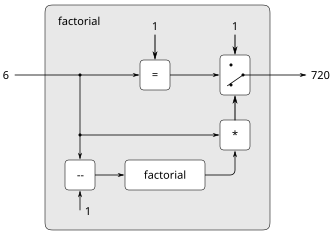
\includegraphics[width=84mm]{assets/figures/chapter_4/figure_4.2.pdf}
\end{imageFigure}

From this perspective, our evaluator is seen to be a \newterm{universal
machine}.  It mimics other machines when these are described as Lisp
programs.\footnote{The fact that the machines are described in Lisp is
inessential.  If we give our evaluator a Lisp program that behaves as an
evaluator for some other language, say C, the Lisp evaluator will emulate the C
evaluator, which in turn can emulate any machine described as a C program.
Similarly, writing a Lisp evaluator in C produces a C program that can execute
any Lisp program.  The deep idea here is that any evaluator can emulate any
other.  Thus, the notion of ``what can in principle be computed'' (ignoring
practicalities of time and memory required) is independent of the language or
the computer, and instead reflects an underlying notion of
\newterm{computability}.  This was first demonstrated in a clear way by Alan
M. Turing (1912-1954), whose 1936 paper laid the foundations for theoretical
computer science.  In the paper, Turing presented a simple computational
model---now known as a \newterm{Turing machine}---and argued that any
``effective process'' can be formulated as a program for such a machine.  (This
argument is known as the \newterm{Church-Turing thesis}.)  Turing then
implemented a universal machine, i.e., a Turing machine that behaves as an
evaluator for Turing-machine programs.  He used this framework to demonstrate
that there are well-posed problems that cannot be computed by Turing machines
(see \link{Exercise 4.15}), and so by implication cannot be formulated as
``effective processes.''  Turing went on to make fundamental contributions to
practical computer science as well.  For example, he invented the idea of
structuring programs using general-purpose subroutines.  See \link{Hodges 1983} for a
biography of Turing.} This is striking. Try to imagine an analogous evaluator
for electrical circuits.  This would be a circuit that takes as input a signal
encoding the plans for some other circuit, such as a filter.  Given this input,
the circuit evaluator would then behave like a filter with the same
description.  Such a universal electrical circuit is almost unimaginably
complex.  It is remarkable that the program evaluator is a rather simple
program.\footnote{Some people find it counterintuitive that an evaluator, which
is implemented by a relatively simple procedure, can emulate programs that are
more complex than the evaluator itself.  The existence of a universal evaluator
machine is a deep and wonderful property of computation.  \newterm{Recursion
theory}, a branch of mathematical logic, is concerned with logical limits of
computation.  Douglas Hofstadter's beautiful book \textit{G\"odel, Escher, Bach}
explores some of these ideas (\link{Hofstadter 1979}).}

% figure 4.3
\begin{imageFigure}{The evaluator emulating a factorial machine.}
  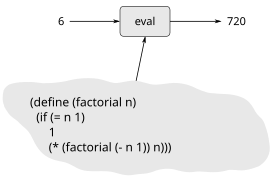
\includegraphics[width=69mm]{assets/figures/chapter_4/figure_4.3.pdf}
\end{imageFigure}

Another striking aspect of the evaluator is that it acts as a bridge between
the data objects that are manipulated by our programming language and the
programming language itself.  Imagine that the evaluator program (implemented
in Lisp) is running, and that a user is typing expressions to the evaluator and
observing the results.  From the perspective of the user, an input expression
such as \code{(* x x)} is an expression in the programming language, which the
evaluator should execute.  From the perspective of the evaluator, however, the
expression is simply a list (in this case, a list of three symbols: \code{*},
\code{x}, and \code{x}) that is to be manipulated according to a well-defined
set of rules.

That the user's programs are the evaluator's data need not be a source of
confusion.  In fact, it is sometimes convenient to ignore this distinction, and
to give the user the ability to explicitly evaluate a data object as a Lisp
expression, by making \code{eval} available for use in programs.  Many Lisp
dialects provide a primitive \code{eval} procedure that takes as arguments an
expression and an environment and evaluates the expression relative to the
environment.\footnote{Warning: This \code{eval} primitive is not identical to
the \code{eval} procedure we implemented in \link{Section 4.1.1}, because it
uses \emph{actual} Scheme environments rather than the sample environment
structures we built in \link{Section 4.1.3}.  These actual environments cannot
be manipulated by the user as ordinary lists; they must be accessed via
\code{eval} or other special operations.  Similarly, the \code{apply} primitive
we saw earlier is not identical to the metacircular \code{apply}, because it
uses actual Scheme procedures rather than the procedure objects we constructed
in \link{Section 4.1.3} and \link{Section 4.1.4}.} Thus,

\begin{codeBlock}
(eval '(* 5 5) user-initial-environment)
\end{codeBlock}

\noindent
and

\begin{codeBlock}
(eval (cons '* (list 5 5)) user-initial-environment)
\end{codeBlock}

\noindent
will both return 25.\footnote{The \acronym{MIT} implementation of Scheme
includes \code{eval}, as well as a symbol \code{user\-/initial\-/environment} that
is bound to the initial environment in which the user's input expressions are
evaluated.}

\begin{exerciseGroup}
\exerciseHeading{\phantomsection\label{Exercise 4.15}Exercise 4.15:} Given a one-argument procedure
\code{p} and an object \code{a}, \code{p} is said to ``halt'' on \code{a} if
evaluating the expression \code{(p a)} returns a value (as opposed to
terminating with an error message or running forever).  Show that it is
impossible to write a procedure \code{halts?} that correctly determines whether
\code{p} halts on \code{a} for any procedure \code{p} and object \code{a}.  Use
the following reasoning: If you had such a procedure \code{halts?}, you could
implement the following program:

\begin{codeBlock}
(define (run-forever) (run-forever))
(define (try p)
  (if (halts? p p) (run-forever) 'halted))
\end{codeBlock}

Now consider evaluating the expression \code{(try try)} and show that any
possible outcome (either halting or running forever) violates the intended
behavior of \code{halts?}.\footnote{Although we stipulated that \code{halts?}
is given a procedure object, notice that this reasoning still applies even if
\code{halts?} can gain access to the procedure's text and its environment.
This is Turing's celebrated \newterm{Halting Theorem}, which gave the first
clear example of a \newterm{non-computable} problem, i.e., a well-posed task
that cannot be carried out as a computational procedure.}
\end{exerciseGroup}

\subsection{Internal Definitions}
\label{Section 4.1.6}

Our environment model of evaluation and our metacircular evaluator execute
definitions in sequence, extending the environment frame one definition at a
time.  This is particularly convenient for interactive program development, in
which the programmer needs to freely mix the application of procedures with the
definition of new procedures.  However, if we think carefully about the
internal definitions used to implement block structure (introduced in
\link{Section 1.1.8}), we will find that name-by-name extension of the environment may
not be the best way to define local variables.

Consider a procedure with internal definitions, such as

\begin{codeBlock}
(define (f x)
  (define (even? n) (if (= n 0) true  (odd?  (- n 1))))
  (define (odd? n)  (if (= n 0) false (even? (- n 1))))
  ~\(\langle \)~~\var{rest of body of \code{f}}~~\(\rangle \)~)
\end{codeBlock}

\noindent
Our intention here is that the name \code{odd?} in the body of the procedure
\code{even?} should refer to the procedure \code{odd?} that is defined after
\code{even?}.  The scope of the name \code{odd?} is the entire body of
\code{f}, not just the portion of the body of \code{f} starting at the point
where the \code{define} for \code{odd?} occurs.  Indeed, when we consider that
\code{odd?} is itself defined in terms of \code{even?}---so that \code{even?}
and \code{odd?} are mutually recursive procedures---we see that the only
satisfactory interpretation of the two \code{define}s is to regard them as if
the names \code{even?} and \code{odd?} were being added to the environment
simultaneously.  More generally, in block structure, the scope of a local name
is the entire procedure body in which the \code{define} is evaluated.

As it happens, our interpreter will evaluate calls to \code{f} correctly, but
for an ``accidental'' reason: Since the definitions of the internal procedures
come first, no calls to these procedures will be evaluated until all of them
have been defined.  Hence, \code{odd?}  will have been defined by the time
\code{even?} is executed.  In fact, our sequential evaluation mechanism will
give the same result as a mechanism that directly implements simultaneous
definition for any procedure in which the internal definitions come first in a
body and evaluation of the value expressions for the defined variables doesn't
actually use any of the defined variables.  (For an example of a procedure that
doesn't obey these restrictions, so that sequential definition isn't equivalent
to simultaneous definition, see \link{Exercise 4.19}.)\footnote{Wanting programs
to not depend on this evaluation mechanism is the reason for the ``management
is not responsible'' remark in \link{Footnote 28} of \link{Chapter 1}.  By
insisting that internal definitions come first and do not use each other while
the definitions are being evaluated, the \acronym{IEEE} standard for Scheme
leaves implementors some choice in the mechanism used to evaluate these
definitions.  The choice of one evaluation rule rather than another here may
seem like a small issue, affecting only the interpretation of ``badly formed''
programs.  However, we will see in \link{Section 5.5.6} that moving to a model
of simultaneous scoping for internal definitions avoids some nasty difficulties
that would otherwise arise in implementing a compiler.}

There is, however, a simple way to treat definitions so that internally defined
names have truly simultaneous scope---just create all local variables that will
be in the current environment before evaluating any of the value expressions.
One way to do this is by a syntax transformation on \code{lambda} expressions.
Before evaluating the body of a \code{lambda} expression, we ``scan out'' and
eliminate all the internal definitions in the body.  The internally defined
variables will be created with a \code{let} and then set to their values by
assignment.  For example, the procedure

\begin{codeBlock}
(lambda ~\(\langle \)~~\var{vars}~~\(\rangle \)~
  (define u ~\(\langle \)~~\var{e1}~~\(\rangle \)~)
  (define v ~\(\langle \)~~\var{e2}~~\(\rangle \)~)
  ~\(\langle \)~~\var{e3}~~\(\rangle \)~)
\end{codeBlock}

\noindent
would be transformed into

\begin{codeBlock}
(lambda ~\(\langle \)~~\var{vars}~~\(\rangle \)~
  (let ((u '*unassigned*)
        (v '*unassigned*))
    (set! u ~\(\langle \)~~\var{e1}~~\(\rangle \)~)
    (set! v ~\(\langle \)~~\var{e2}~~\(\rangle \)~)
    ~\(\langle \)~~\var{e3}~~\(\rangle \)~))
\end{codeBlock}

\noindent
where \code{*unassigned*} is a special symbol that causes looking up a variable
to signal an error if an attempt is made to use the value of the
not-yet-assigned variable.

An alternative strategy for scanning out internal definitions is shown in
\link{Exercise 4.18}.  Unlike the transformation shown above, this enforces the
restriction that the defined variables' values can be evaluated without using
any of the variables' values.\footnote{The \acronym{IEEE} standard for Scheme
allows for different implementation strategies by specifying that it is up to
the programmer to obey this restriction, not up to the implementation to
enforce it.  Some Scheme implementations, including \acronym{MIT} Scheme, use
the transformation shown above.  Thus, some programs that don't obey this
restriction will in fact run in such implementations.}

\begin{exerciseGroup}
\exerciseHeading{\phantomsection\label{Exercise 4.16}Exercise 4.16:} In this exercise we implement the
method just described for interpreting internal definitions.  We assume that
the evaluator supports \code{let} (see \link{Exercise 4.6}).

\begin{enumerate}[a.]

\item
Change \code{lookup\-/variable\-/value} (\link{Section 4.1.3}) to signal an error if
the value it finds is the symbol \code{*unassigned*}.

\item
Write a procedure \code{scan\-/out\-/defines} that takes a procedure body and
returns an equivalent one that has no internal definitions, by making the
transformation described above.

\item
Install \code{scan\-/out\-/defines} in the interpreter, either in
\code{make\-/procedure} or in \code{procedure\-/body} (see \link{Section 4.1.3}).
Which place is better?  Why?

\end{enumerate}

\exerciseHeading{\phantomsection\label{Exercise 4.17}Exercise 4.17:} Draw diagrams of the environment
in effect when evaluating the expression \( \langle \)\var{e3}\( \kern0.1em\rangle \) in the procedure in the
text, comparing how this will be structured when definitions are interpreted
sequentially with how it will be structured if definitions are scanned out as
described.  Why is there an extra frame in the transformed program?  Explain
why this difference in environment structure can never make a difference in the
behavior of a correct program.  Design a way to make the interpreter implement
the ``simultaneous'' scope rule for internal definitions without constructing
the extra frame.

\exerciseHeading{\phantomsection\label{Exercise 4.18}Exercise 4.18:} Consider an alternative strategy
for scanning out definitions that translates the example in the text to

\begin{codeBlock}
(lambda ~\(\langle \)~~\var{vars}~~\(\rangle \)~
  (let ((u '*unassigned*) (v '*unassigned*))
    (let ((a ~\(\langle \)~~\var{e1}~~\(\rangle \)~) (b ~\(\langle \)~~\var{e2}~~\(\rangle \)~))
      (set! u a)
      (set! v b))
    ~\(\langle \)~~\var{e3}~~\(\rangle \)~))
\end{codeBlock}

Here \code{a} and \code{b} are meant to represent new variable names, created
by the interpreter, that do not appear in the user's program.  Consider the
\code{solve} procedure from \link{Section 3.5.4}:

\begin{codeBlock}
(define (solve f y0 dt)
  (define  y (integral (delay dy) y0 dt))
  (define dy (stream-map f y))
  y)
\end{codeBlock}

Will this procedure work if internal definitions are scanned out as shown in
this exercise?  What if they are scanned out as shown in the text?  Explain.

\exerciseHeading{\phantomsection\label{Exercise 4.19}Exercise 4.19:} Ben Bitdiddle, Alyssa P. Hacker,
and Eva Lu Ator are arguing about the desired result of evaluating the
expression

\begin{codeBlock}
(let ((a 1))
  (define (f x)
    (define b (+ a x))
    (define a 5)
    (+ a b))
  (f 10))
\end{codeBlock}

Ben asserts that the result should be obtained using the sequential rule for
\code{define}: \code{b} is defined to be 11, then \code{a} is defined to be 5,
so the result is 16.  Alyssa objects that mutual recursion requires the
simultaneous scope rule for internal procedure definitions, and that it is
unreasonable to treat procedure names differently from other names.  Thus, she
argues for the mechanism implemented in \link{Exercise 4.16}.  This would lead
to \code{a} being unassigned at the time that the value for \code{b} is to be
computed.  Hence, in Alyssa's view the procedure should produce an error.  Eva
has a third opinion.  She says that if the definitions of \code{a} and \code{b}
are truly meant to be simultaneous, then the value 5 for \code{a} should be
used in evaluating \code{b}.  Hence, in Eva's view \code{a} should be 5,
\code{b} should be 15, and the result should be 20.  Which (if any) of these
viewpoints do you support?  Can you devise a way to implement internal
definitions so that they behave as Eva prefers?\footnote{The \acronym{MIT}
implementors of Scheme support Alyssa on the following grounds: Eva is in
principle correct---the definitions should be regarded as simultaneous.  But
it seems difficult to implement a general, efficient mechanism that does what
Eva requires.  In the absence of such a mechanism, it is better to generate an
error in the difficult cases of simultaneous definitions (Alyssa's notion) than
to produce an incorrect answer (as Ben would have it).}

\exerciseHeading{\phantomsection\label{Exercise 4.20}Exercise 4.20:} Because internal definitions look
sequential but are actually simultaneous, some people prefer to avoid them
entirely, and use the special form \code{letrec} instead.  \code{letrec} looks
like \code{let}, so it is not surprising that the variables it binds are bound
simultaneously and have the same scope as each other.  The sample procedure
\code{f} above can be written without internal definitions, but with exactly
the same meaning, as

\begin{codeBlock}
(define (f x)
  (letrec
    ((even? (lambda (n)
              (if (= n 0) true  (odd?  (- n 1)))))
     (odd?  (lambda (n)
              (if (= n 0) false (even? (- n 1))))))
    ~\(\langle \)~~\var{rest of body of \code{f}}~~\(\rangle \)~))
\end{codeBlock}

\code{letrec} expressions, which have the form

\begin{codeBlock}
(letrec ((~\(\langle \)~~\var{var}~~\(_{\mono{1}}\rangle \)~ ~\(\langle \)~~\var{exp}~~\(_{\mono{1}}\rangle \)~) ~\( \dots \)~ (~\(\langle \)~~\var{var}~~\(_{\monoItalic{n}}\rangle \)~ ~\(\langle \)~~\var{exp}~~\(_{\monoItalic{n}}\rangle \)~))
  ~\(\langle \)~~\var{body}~~\(\rangle \)~)
\end{codeBlock}

\noindent
are a variation on \code{let} in which the expressions
\( \langle \)\var{exp}\( _k\rangle \) that provide the initial values for the
variables \( \langle \)\var{var}\( _k\rangle \) are evaluated in an environment
that includes all the \code{letrec} bindings.  This permits recursion in the
bindings, such as the mutual recursion of \code{even?} and \code{odd?} in the
example above, or the evaluation of 10 factorial with

\begin{codeBlock}
(letrec
  ((fact (lambda (n)
           (if (= n 1) 1 (* n (fact (- n 1)))))))
  (fact 10))
\end{codeBlock}

\begin{enumerate}[a.]

\item
Implement \code{letrec} as a derived expression, by transforming a
\code{letrec} expression into a \code{let} expression as shown in the text
above or in \link{Exercise 4.18}.  That is, the \code{letrec} variables should
be created with a \code{let} and then be assigned their values with
\code{set!}.

\item
Louis Reasoner is confused by all this fuss about internal definitions.  The
way he sees it, if you don't like to use \code{define} inside a procedure, you
can just use \code{let}.  Illustrate what is loose about his reasoning by
drawing an environment diagram that shows the environment in which the
\( \langle \)\var{rest of body of \code{f}}\( \kern0.08em\rangle \) is evaluated during evaluation of the
expression \code{(f 5)}, with \code{f} defined as in this exercise.  Draw an
environment diagram for the same evaluation, but with \code{let} in place of
\code{letrec} in the definition of \code{f}.

\end{enumerate}

\exerciseHeading{\phantomsection\label{Exercise 4.21}Exercise 4.21:} Amazingly,
Louis's intuition in \link{Exercise 4.20} is correct. It is indeed possible to
specify recursive procedures without using \code{letrec} (or even \code{define}),
although the method for accomplishing this is much more subtle than Louis imagined.
The following expression computes 10 factorial by applying a recursive factorial
procedure:\footnote{This example illustrates a programming trick for
formulating recursive procedures without using \code{define}.  The most general
trick of this sort is the \( Y \) \newterm{operator}, which can be used to give a
``pure λ-calculus'' implementation of recursion.  (See \link{Stoy 1977} for
details on the λ-calculus, and \link{Gabriel 1988} for an exposition of the
\( Y \) operator in Scheme.)}

\begin{codeBlock}
((lambda (n)
   ((lambda (fact) (fact fact n))
    (lambda (ft k) (if (= k 1)
                       1
                       (* k (ft ft (- k 1)))))))
 10)
\end{codeBlock}

\begin{enumerate}[a.]

\item
Check (by evaluating the expression) that this really does compute factorials.
Devise an analogous expression for computing Fibonacci numbers.

\item
Consider the following procedure, which includes mutually recursive internal
definitions:

\begin{codeBlock}
(define (f x)
  (define (even? n)
    (if (= n 0) true  (odd?  (- n 1))))
  (define (odd? n)
    (if (= n 0) false (even? (- n 1))))
  (even? x))
\end{codeBlock}

Fill in the missing expressions to complete an alternative definition of
\code{f}, which uses neither internal definitions nor \code{letrec}:

\begin{codeBlock}
(define (f x)
  ((lambda (even? odd?) (even? even? odd? x))
   (lambda (ev? od? n)
     (if (= n 0) true (od? ~\(\langle \)~??~\(\rangle \)~ ~\(\langle \)~??~\(\rangle \)~ ~\(\langle \)~??~\(\rangle \)~)))
   (lambda (ev? od? n)
     (if (= n 0) false (ev? ~\(\langle \)~??~\(\rangle \)~ ~\(\langle \)~??~\(\rangle \)~ ~\(\langle \)~??~\(\rangle \)~)))))
\end{codeBlock}
\end{enumerate}
\end{exerciseGroup}

\subsection{Separating Syntactic Analysis from Execution}
\label{Section 4.1.7}

The evaluator implemented above is simple, but it is very inefficient, because
the syntactic analysis of expressions is interleaved with their execution.
Thus if a program is executed many times, its syntax is analyzed many times.
Consider, for example, evaluating \code{(factorial 4)} using the following
definition of \code{factorial}:

\begin{codeBlock}
(define (factorial n)
  (if (= n 1) 1 (* (factorial (- n 1)) n)))
\end{codeBlock}

\noindent
Each time \code{factorial} is called, the evaluator must determine that the
body is an \code{if} expression and extract the predicate.  Only then can it
evaluate the predicate and dispatch on its value.  Each time it evaluates the
expression \code{(* (factorial (- n 1)) n)}, or the subexpressions
\code{(factorial (- n 1))} and \code{(- n 1)}, the evaluator must perform the
case analysis in \code{eval} to determine that the expression is an
application, and must extract its operator and operands.  This analysis is
expensive.  Performing it repeatedly is wasteful.

We can transform the evaluator to be significantly more efficient by arranging
things so that syntactic analysis is performed only once.\footnote{This
technique is an integral part of the compilation process, which we shall
discuss in \link{Chapter 5}.  Jonathan Rees wrote a Scheme interpreter like this
in about 1982 for the T project (\link{Rees and Adams 1982}).  Marc \link{Feeley (1986)} (see
also \link{Feeley and Lapalme 1987}) independently invented this technique in his
master's thesis.} We split \code{eval}, which takes an expression and an
environment, into two parts.  The procedure \code{analyze} takes only the
expression.  It performs the syntactic analysis and returns a new procedure,
the \newterm{execution procedure}, that encapsulates the work to be done in
executing the analyzed expression.  The execution procedure takes an
environment as its argument and completes the evaluation.  This saves work
because \code{analyze} will be called only once on an expression, while the
execution procedure may be called many times.

With the separation into analysis and execution, \code{eval} now becomes

\begin{codeBlock}
(define (eval exp env) ((analyze exp) env))
\end{codeBlock}

\noindent
The result of calling \code{analyze} is the execution procedure to be applied
to the environment.  The \code{analyze} procedure is the same case analysis as
performed by the original \code{eval} of \link{Section 4.1.1}, except that the
procedures to which we dispatch perform only analysis, not full evaluation:

\begin{codeBlock}
(define (analyze exp)
  (cond ((self-evaluating? exp)
          (analyze-self-evaluating exp))
        ((quoted? exp) (analyze-quoted exp))
        ((variable? exp) (analyze-variable exp))
        ((assignment? exp) (analyze-assignment exp))
        ((definition? exp) (analyze-definition exp))
        ((if? exp) (analyze-if exp))
        ((lambda? exp) (analyze-lambda exp))
        ((begin? exp)
          (analyze-sequence (begin-actions exp)))
        ((cond? exp) (analyze (cond->if exp)))
        ((application? exp) (analyze-application exp))
        (else
          (error "Unknown expression type: ANALYZE" exp))))
\end{codeBlock}

\noindent
Here is the simplest syntactic analysis procedure, which handles
self-evaluating expressions.  It returns an execution procedure that ignores
its environment argument and just returns the expression:

\begin{codeBlock}
(define (analyze-self-evaluating exp)
  (lambda (env) exp))
\end{codeBlock}

\noindent
For a quoted expression, we can gain a little efficiency by extracting the text
of the quotation only once, in the analysis phase, rather than in the execution
phase.

\begin{codeBlock}
(define (analyze-quoted exp)
  (let ((qval (text-of-quotation exp)))
    (lambda (env) qval)))
\end{codeBlock}

\noindent
Looking up a variable value must still be done in the execution phase, since
this depends upon knowing the environment.\footnote{There is, however, an
important part of the variable search that \emph{can} be done as part of the
syntactic analysis.  As we will show in \link{Section 5.5.6}, one can determine
the position in the environment structure where the value of the variable will
be found, thus obviating the need to scan the environment for the entry that
matches the variable.}

\begin{codeBlock}
(define (analyze-variable exp)
  (lambda (env) (lookup-variable-value exp env)))
\end{codeBlock}

\noindent
\code{analyze\-/assignment} also must defer actually setting the variable until
the execution, when the environment has been supplied.  However, the fact that
the \code{assignment\-/value} expression can be analyzed (recursively) during
analysis is a major gain in efficiency, because the \code{assignment\-/value}
expression will now be analyzed only once.  The same holds true for
definitions.

\begin{codeBlock}
(define (analyze-assignment exp)
  (let ((var (assignment-variable exp))
        (vproc (analyze (assignment-value exp))))
    (lambda (env)
      (set-variable-value! var (vproc env) env)
      'ok)))
(define (analyze-definition exp)
  (let ((var (definition-variable exp))
        (vproc (analyze (definition-value exp))))
    (lambda (env)
      (define-variable! var (vproc env) env)
      'ok)))
\end{codeBlock}

\noindent
For \code{if} expressions, we extract and analyze the predicate, consequent,
and alternative at analysis time.

\begin{codeBlock}
(define (analyze-if exp)
  (let ((pproc (analyze (if-predicate exp)))
        (cproc (analyze (if-consequent exp)))
        (aproc (analyze (if-alternative exp))))
    (lambda (env) (if (true? (pproc env))
                      (cproc env)
                      (aproc env)))))
\end{codeBlock}

\noindent
Analyzing a \code{lambda} expression also achieves a major gain in efficiency:
We analyze the \code{lambda} body only once, even though procedures resulting
from evaluation of the \code{lambda} may be applied many times.

\begin{codeBlock}
(define (analyze-lambda exp)
  (let ((vars (lambda-parameters exp))
        (bproc (analyze-sequence (lambda-body exp))))
    (lambda (env) (make-procedure vars bproc env))))
\end{codeBlock}

\noindent
Analysis of a sequence of expressions (as in a \code{begin} or the body of a
\code{lambda} expression) is more involved.\footnote{See \link{Exercise 4.23}
for some insight into the processing of sequences.} Each expression in the
sequence is analyzed, yielding an execution procedure.  These execution
procedures are combined to produce an execution procedure that takes an
environment as argument and sequentially calls each individual execution
procedure with the environment as argument.

\begin{codeBlock}
(define (analyze-sequence exps)
  (define (sequentially proc1 proc2)
    (lambda (env) (proc1 env) (proc2 env)))
  (define (loop first-proc rest-procs)
    (if (null? rest-procs)
        first-proc
        (loop (sequentially first-proc
                            (car rest-procs))
              (cdr rest-procs))))
  (let ((procs (map analyze exps)))
    (if (null? procs)
      (error "Empty sequence: ANALYZE"))
    (loop (car procs) (cdr procs))))
\end{codeBlock}

\noindent
To analyze an application, we analyze the operator and operands and construct
an execution procedure that calls the operator execution procedure (to obtain
the actual procedure to be applied) and the operand execution procedures (to
obtain the actual arguments).  We then pass these to
\code{execute\-/application}, which is the analog of \code{apply} in
\link{Section 4.1.1}.  \code{execute\-/application} differs from \code{apply} in that the
procedure body for a compound procedure has already been analyzed, so there is
no need to do further analysis.  Instead, we just call the execution procedure
for the body on the extended environment.

\begin{codeBlock}
(define (analyze-application exp)
  (let ((fproc (analyze (operator exp)))
        (aprocs (map analyze (operands exp))))
    (lambda (env)
      (execute-application
       (fproc env)
       (map (lambda (aproc) (aproc env))
            aprocs)))))
(define (execute-application proc args)
  (cond ((primitive-procedure? proc)
         (apply-primitive-procedure proc args))
        ((compound-procedure? proc)
         ((procedure-body proc)
          (extend-environment
           (procedure-parameters proc)
           args
           (procedure-environment proc))))
        (else
         (error "Unknown procedure type: EXECUTE-APPLICATION"
                proc))))
\end{codeBlock}

\noindent
Our new evaluator uses the same data structures, syntax procedures, and
run-time support procedures as in sections \link{Section 4.1.2}, \link{Section 4.1.3}, and
\link{Section 4.1.4}.

\begin{exerciseGroup}
\exerciseHeading{\phantomsection\label{Exercise 4.22}Exercise 4.22:} Extend the evaluator in this
section to support the special form \code{let}.  (See \link{Exercise 4.6}.)

\exerciseHeading{\phantomsection\label{Exercise 4.23}Exercise 4.23:} Alyssa P. Hacker doesn't
understand why \code{analyze\-/sequence} needs to be so complicated.  All the
other analysis procedures are straightforward transformations of the
corresponding evaluation procedures (or \code{eval} clauses) in
\link{Section 4.1.1}.  She expected \code{analyze\-/sequence} to look like this:

\begin{codeBlock}
(define (analyze-sequence exps)
  (define (execute-sequence procs env)
    (cond ((null? (cdr procs))
           ((car procs) env))
          (else
           ((car procs) env)
           (execute-sequence (cdr procs) env))))
  (let ((procs (map analyze exps)))
    (if (null? procs)
        (error "Empty sequence: ANALYZE"))
    (lambda (env)
      (execute-sequence procs env))))
\end{codeBlock}

Eva Lu Ator explains to Alyssa that the version in the text does more of the
work of evaluating a sequence at analysis time.  Alyssa's sequence-execution
procedure, rather than having the calls to the individual execution procedures
built in, loops through the procedures in order to call them: In effect,
although the individual expressions in the sequence have been analyzed, the
sequence itself has not been.

Compare the two versions of \code{analyze\-/sequence}.  For example, consider the
common case (typical of procedure bodies) where the sequence has just one
expression.  What work will the execution procedure produced by Alyssa's
program do?  What about the execution procedure produced by the program in the
text above?  How do the two versions compare for a sequence with two
expressions?

\exerciseHeading{\phantomsection\label{Exercise 4.24}Exercise 4.24:} Design and carry out some
experiments to compare the speed of the original metacircular evaluator with
the version in this section.  Use your results to estimate the fraction of time
that is spent in analysis versus execution for various procedures.
\end{exerciseGroup}

\section{Variations on a Scheme - Lazy Evaluation}
\label{Section 4.2}

Now that we have an evaluator expressed as a Lisp program, we can experiment
with alternative choices in language design simply by modifying the evaluator.
Indeed, new languages are often invented by first writing an evaluator that
embeds the new language within an existing high-level language.  For example,
if we wish to discuss some aspect of a proposed modification to Lisp with
another member of the Lisp community, we can supply an evaluator that embodies
the change.  The recipient can then experiment with the new evaluator and send
back comments as further modifications.  Not only does the high-level
implementation base make it easier to test and debug the evaluator; in
addition, the embedding enables the designer to snarf\,\footnote{Snarf: ``To
grab, especially a large document or file for the purpose of using it either
with or without the owner's permission.''  Snarf down: ``To snarf, sometimes
with the connotation of absorbing, processing, or understanding.''  (These
definitions were snarfed from \link{Steele et al. 1983}.  See also \link{Raymond 1993}.)}
features from the underlying language, just as our embedded Lisp evaluator uses
primitives and control structure from the underlying Lisp.  Only later (if
ever) need the designer go to the trouble of building a complete implementation
in a low-level language or in hardware.  In this section and the next we
explore some variations on Scheme that provide significant additional
expressive power.



\subsection{Normal Order and Applicative Order}
\label{Section 4.2.1}

In \link{Section 1.1}, where we began our discussion of models of evaluation, we
noted that Scheme is an \newterm{applicative-order} language, namely, that all
the arguments to Scheme procedures are evaluated when the procedure is applied.
In contrast, \newterm{normal-order} languages delay evaluation of procedure
arguments until the actual argument values are needed.  Delaying evaluation of
procedure arguments until the last possible moment (e.g., until they are
required by a primitive operation) is called \newterm{lazy
evaluation}.\footnote{The difference between the ``lazy'' terminology and the
``normal-order'' terminology is somewhat fuzzy.  Generally, ``lazy'' refers to
the mechanisms of particular evaluators, while ``normal-order'' refers to the
semantics of languages, independent of any particular evaluation strategy.  But
this is not a hard-and-fast distinction, and the two terminologies are often
used interchangeably.}  Consider the procedure

\begin{codeBlock}
(define (try a b) (if (= a 0) 1 b))
\end{codeBlock}

\noindent
Evaluating \code{(try 0 (/ 1 0))} generates an error in Scheme.  With lazy
evaluation, there would be no error.  Evaluating the expression would return 1,
because the argument \code{(/ 1 0)} would never be evaluated.

An example that exploits lazy evaluation is the definition of a procedure
\code{unless}

\begin{codeBlock}
(define (unless condition usual-value exceptional-value)
  (if condition exceptional-value usual-value))
\end{codeBlock}

\noindent
that can be used in expressions such as

\begin{codeBlock}
(unless (= b 0)
        (/ a b)
        (begin (display "exception: returning 0") 0))
\end{codeBlock}

\noindent
This won't work in an applicative-order language because both the usual value
and the exceptional value will be evaluated before \code{unless} is called
(compare \link{Exercise 1.6}).  An advantage of lazy evaluation is that some
procedures, such as \code{unless}, can do useful computation even if evaluation
of some of their arguments would produce errors or would not terminate.

If the body of a procedure is entered before an argument has been evaluated we
say that the procedure is \newterm{non-strict} in that argument.  If the
argument is evaluated before the body of the procedure is entered we say that
the procedure is \newterm{strict} in that argument.\footnote{The ``strict''
versus ``non-strict'' terminology means essentially the same thing as
``applicative-order'' versus ``normal-order,'' except that it refers to
individual procedures and arguments rather than to the language as a whole.  At
a conference on programming languages you might hear someone say, ``The
normal-order language Hassle has certain strict primitives.  Other procedures
take their arguments by lazy evaluation.''}  In a purely applicative-order
language, all procedures are strict in each argument.  In a purely normal-order
language, all compound procedures are non-strict in each argument, and
primitive procedures may be either strict or non-strict.  There are also
languages (see \link{Exercise 4.31}) that give programmers detailed control over
the strictness of the procedures they define.

A striking example of a procedure that can usefully be made non-strict is
\code{cons} (or, in general, almost any constructor for data structures).  One
can do useful computation, combining elements to form data structures and
operating on the resulting data structures, even if the values of the elements
are not known.  It makes perfect sense, for instance, to compute the length of
a list without knowing the values of the individual elements in the list.  We
will exploit this idea in \link{Section 4.2.3} to implement the streams of
\link{Chapter 3} as lists formed of non-strict \code{cons} pairs.

\begin{exerciseGroup}
\exerciseHeading{\phantomsection\label{Exercise 4.25}Exercise 4.25:} Suppose that (in ordinary
applicative-order Scheme) we define \code{unless} as shown above and then
define \code{factorial} in terms of \code{unless} as

\begin{codeBlock}
(define (factorial n)
  (unless (= n 1)
          (* n (factorial (- n 1)))
          1))
\end{codeBlock}

What happens if we attempt to evaluate \code{(factorial 5)}?  Will our
definitions work in a normal-order language?

\exerciseHeading{\phantomsection\label{Exercise 4.26}Exercise 4.26:} Ben Bitdiddle and Alyssa
P. Hacker disagree over the importance of lazy evaluation for implementing
things such as \code{unless}.  Ben points out that it's possible to implement
\code{unless} in applicative order as a special form.  Alyssa counters that, if
one did that, \code{unless} would be merely syntax, not a procedure that could
be used in conjunction with higher-order procedures.  Fill in the details on
both sides of the argument.  Show how to implement \code{unless} as a derived
expression (like \code{cond} or \code{let}), and give an example of a situation
where it might be useful to have \code{unless} available as a procedure, rather
than as a special form.
\end{exerciseGroup}

\subsection{An Interpreter with Lazy Evaluation}
\label{Section 4.2.2}

In this section we will implement a normal-order language that is the same as
Scheme except that compound procedures are non-strict in each argument.
Primitive procedures will still be strict.  It is not difficult to modify the
evaluator of \link{Section 4.1.1} so that the language it interprets behaves
this way.  Almost all the required changes center around procedure application.

The basic idea is that, when applying a procedure, the interpreter must
determine which arguments are to be evaluated and which are to be delayed.  The
delayed arguments are not evaluated; instead, they are transformed into objects
called \newterm{thunks}.\footnote{The word \newterm{thunk} was invented by an
informal working group that was discussing the implementation of call-by-name
in Algol 60.  They observed that most of the analysis of (``thinking about'')
the expression could be done at compile time; thus, at run time, the expression
would already have been ``thunk'' about (\link{Ingerman et al. 1960}).} The thunk must
contain the information required to produce the value of the argument when it
is needed, as if it had been evaluated at the time of the application.  Thus,
the thunk must contain the argument expression and the environment in which the
procedure application is being evaluated.

The process of evaluating the expression in a thunk is called
\newterm{forcing}.\footnote{This is analogous to the use of \code{force} on the
delayed objects that were introduced in \link{Chapter 3} to represent streams.
The critical difference between what we are doing here and what we did in
\link{Chapter 3} is that we are building delaying and forcing into the
evaluator, and thus making this uniform and automatic throughout the language.}
In general, a thunk will be forced only when its value is needed: when it is
passed to a primitive procedure that will use the value of the thunk; when it
is the value of a predicate of a conditional; and when it is the value of an
operator that is about to be applied as a procedure.  One design choice we have
available is whether or not to \newterm{memoize} thunks, as we did with delayed
objects in \link{Section 3.5.1}.  With memoization, the first time a thunk is
forced, it stores the value that is computed.  Subsequent forcings simply
return the stored value without repeating the computation.  We'll make our
interpreter memoize, because this is more efficient for many applications.
There are tricky considerations here, however.\footnote{Lazy evaluation
combined with memoization is sometimes referred to as \newterm{call-by-need}
argument passing, in contrast to \newterm{call-by-name} argument passing.
(Call-by-name, introduced in Algol 60, is similar to non-memoized lazy
evaluation.)  As language designers, we can build our evaluator to memoize, not
to memoize, or leave this an option for programmers (\link{Exercise 4.31}).  As
you might expect from \link{Chapter 3}, these choices raise issues that become
both subtle and confusing in the presence of assignments.  (See \link{Exercise 4.27}
and \link{Exercise 4.29}.)  An excellent article by \link{Clinger (1982)}
attempts to clarify the multiple dimensions of confusion that arise here.}

\subsubsection*{Modifying the evaluator}

The main difference between the lazy evaluator and the one in \link{Section 4.1}
is in the handling of procedure applications in \code{eval} and \code{apply}.

The \code{application?} clause of \code{eval} becomes

\begin{codeBlock}
((application? exp)
 (apply (actual-value (operator exp) env)
        (operands exp)
        env))
\end{codeBlock}

\noindent
This is almost the same as the \code{application?} clause of \code{eval} in
\link{Section 4.1.1}.  For lazy evaluation, however, we call \code{apply} with
the operand expressions, rather than the arguments produced by evaluating them.
Since we will need the environment to construct thunks if the arguments are to
be delayed, we must pass this as well.  We still evaluate the operator, because
\code{apply} needs the actual procedure to be applied in order to dispatch on
its type (primitive versus compound) and apply it.

Whenever we need the actual value of an expression, we use

\begin{codeBlock}
(define (actual-value exp env)
  (force-it (eval exp env)))
\end{codeBlock}

\noindent
instead of just \code{eval}, so that if the expression's value is a thunk, it
will be forced.

Our new version of \code{apply} is also almost the same as the version in
\link{Section 4.1.1}.  The difference is that \code{eval} has passed in
unevaluated operand expressions: For primitive procedures (which are strict),
we evaluate all the arguments before applying the primitive; for compound
procedures (which are non-strict) we delay all the arguments before applying
the procedure.

\begin{codeBlock}
(define (apply procedure arguments env)
  (cond ((primitive-procedure? procedure)
         (apply-primitive-procedure
          procedure
          (list-of-arg-values arguments env)))   ~\textrm{; changed}~
        ((compound-procedure? procedure)
         (eval-sequence
          (procedure-body procedure)
          (extend-environment
           (procedure-parameters procedure)
           (list-of-delayed-args arguments env)  ~\textrm{; changed}~
           (procedure-environment procedure))))
        (else (error "Unknown procedure type: APPLY"
                     procedure))))
\end{codeBlock}

\noindent
The procedures that process the arguments are just like \code{list\-/of\-/values}
from \link{Section 4.1.1}, except that \code{list\-/of\-/delayed\-/args} delays the
arguments instead of evaluating them, and \code{list\-/of\-/arg\-/values} uses
\code{actual\-/value} instead of \code{eval}:

\begin{codeBlock}
(define (list-of-arg-values exps env)
  (if (no-operands? exps)
      '()
      (cons (actual-value (first-operand exps)
                          env)
            (list-of-arg-values (rest-operands exps)
                                env))))
(define (list-of-delayed-args exps env)
  (if (no-operands? exps)
      '()
      (cons (delay-it (first-operand exps)
                      env)
            (list-of-delayed-args (rest-operands exps)
                                  env))))
\end{codeBlock}

\noindent
The other place we must change the evaluator is in the handling of \code{if},
where we must use \code{actual\-/value} instead of \code{eval} to get the value
of the predicate expression before testing whether it is true or false:

\begin{codeBlock}
(define (eval-if exp env)
  (if (true? (actual-value (if-predicate exp) env))
      (eval (if-consequent exp) env)
      (eval (if-alternative exp) env)))
\end{codeBlock}

\noindent
Finally, we must change the \code{driver\-/loop} procedure (\link{Section 4.1.4})
to use \code{actual\-/value} instead of \code{eval}, so that if a delayed value
is propagated back to the read-eval-print loop, it will be forced before being
printed.  We also change the prompts to indicate that this is the lazy
evaluator:

\begin{codeBlock}
(define input-prompt  ";;; L-Eval input:")
(define output-prompt ";;; L-Eval value:")
(define (driver-loop)
  (prompt-for-input input-prompt)
  (let ((input (read)))
    (let ((output
           (actual-value
            input the-global-environment)))
      (announce-output output-prompt)
      (user-print output)))
  (driver-loop))
\end{codeBlock}

\noindent
With these changes made, we can start the evaluator and test it.  The
successful evaluation of the \code{try} expression discussed in
\link{Section 4.2.1} indicates that the interpreter is performing lazy evaluation:

\begin{codeBlock}
(define the-global-environment (setup-environment))
(driver-loop)
~\textit{;;; L-Eval input:}~
(define (try a b) (if (= a 0) 1 b))
~\textit{;;; L-Eval value:}~
~\textit{ok}~
~\textit{;;; L-Eval input:}~
(try 0 (/ 1 0))
~\textit{;;; L-Eval value:}~
~\textit{1}~
\end{codeBlock}

\subsubsection*{Representing thunks}

Our evaluator must arrange to create thunks when procedures are applied to
arguments and to force these thunks later.  A thunk must package an expression
together with the environment, so that the argument can be produced later.  To
force the thunk, we simply extract the expression and environment from the
thunk and evaluate the expression in the environment.  We use
\code{actual\-/value} rather than \code{eval} so that in case the value of the
expression is itself a thunk, we will force that, and so on, until we reach
something that is not a thunk:

\begin{codeBlock}
(define (force-it obj)
  (if (thunk? obj)
      (actual-value (thunk-exp obj) (thunk-env obj))
      obj))
\end{codeBlock}

\noindent
One easy way to package an expression with an environment is to make a list
containing the expression and the environment.  Thus, we create a thunk as
follows:

\begin{codeBlock}
(define (delay-it exp env)
  (list 'thunk exp env))
(define (thunk? obj)
  (tagged-list? obj 'thunk))
(define (thunk-exp thunk) (cadr  thunk))
(define (thunk-env thunk) (caddr thunk))
\end{codeBlock}

\noindent
Actually, what we want for our interpreter is not quite this, but rather thunks
that have been memoized.  When a thunk is forced, we will turn it into an
evaluated thunk by replacing the stored expression with its value and changing
the \code{thunk} tag so that it can be recognized as already
evaluated.\footnote{Notice that we also erase the \code{env} from the thunk
once the expression's value has been computed.  This makes no difference in the
values returned by the interpreter.  It does help save space, however, because
removing the reference from the thunk to the \code{env} once it is no longer
needed allows this structure to be \newterm{garbage-collected} and its space
recycled, as we will discuss in \link{Section 5.3}.

Similarly, we could have allowed unneeded environments in the memoized delayed
objects of \link{Section 3.5.1} to be garbage-collected, by having
\code{memo\-/proc} do something like \code{(set! proc '())} to discard the
procedure \code{proc} (which includes the environment in which the \code{delay}
was evaluated) after storing its value.}

\begin{codeBlock}
(define (evaluated-thunk? obj)
  (tagged-list? obj 'evaluated-thunk))
(define (thunk-value evaluated-thunk)
  (cadr evaluated-thunk))
(define (force-it obj)
  (cond ((thunk? obj)
         (let ((result (actual-value (thunk-exp obj)
                                     (thunk-env obj))))
           (set-car! obj 'evaluated-thunk)
           (set-car! (cdr obj)
                     result)     ~\textrm{; replace \code{exp} with its value}~
           (set-cdr! (cdr obj)
                     '())        ~\textrm{; forget unneeded \code{env}}~
           result))
        ((evaluated-thunk? obj) (thunk-value obj))
        (else obj)))
\end{codeBlock}

\noindent
Notice that the same \code{delay\-/it} procedure works both with and without
memoization.

\begin{exerciseGroup}
\exerciseHeading{\phantomsection\label{Exercise 4.27}Exercise 4.27:} Suppose we type in the following
definitions to the lazy evaluator:

\begin{codeBlock}
(define count 0)
(define (id x) (set! count (+ count 1)) x)
\end{codeBlock}

Give the missing values in the following sequence of interactions, and explain
your answers.\footnote{This exercise demonstrates that the interaction between
lazy evaluation and side effects can be very confusing.  This is just what you
might expect from the discussion in \link{Chapter 3}.}

\begin{codeBlock}
(define w (id (id 10)))
~\textit{;;; L-Eval input:}~
count
~\textit{;;; L-Eval value:}~
~\(\langle \)~~\var{response}~~\(\rangle \)~
~\textit{;;; L-Eval input:}~
w
~\textit{;;; L-Eval value:}~
~\(\langle \)~~\var{response}~~\(\rangle \)~
~\textit{;;; L-Eval input:}~
count
~\textit{;;; L-Eval value:}~
~\(\langle \)~~\var{response}~~\(\rangle \)~
\end{codeBlock}

\exerciseHeading{\phantomsection\label{Exercise 4.28}Exercise 4.28:} \code{eval} uses
\code{actual\-/value} rather than \code{eval} to evaluate the operator before
passing it to \code{apply}, in order to force the value of the operator.  Give
an example that demonstrates the need for this forcing.

\noindent
\exerciseHeading{\phantomsection\label{Exercise 4.29}Exercise 4.29:} Exhibit a program that you would
expect to run much more slowly without memoization than with memoization.
Also, consider the following interaction, where the \code{id} procedure is
defined as in \link{Exercise 4.27} and \code{count} starts at 0:

\begin{codeBlock}
(define (square x) (* x x))
~\textit{;;; L-Eval input:}~
(square (id 10))
~\textit{;;; L-Eval value:}~
~\(\langle \)~~\var{response}~~\(\rangle \)~
~\textit{;;; L-Eval input:}~
count
~\textit{;;; L-Eval value:}~
~\(\langle \)~~\var{response}~~\(\rangle \)~
\end{codeBlock}

Give the responses both when the evaluator memoizes and when it does not.

\exerciseHeading{\phantomsection\label{Exercise 4.30}Exercise 4.30:} Cy D. Fect, a reformed C
programmer, is worried that some side effects may never take place, because the
lazy evaluator doesn't force the expressions in a sequence.  Since the value of
an expression in a sequence other than the last one is not used (the expression
is there only for its effect, such as assigning to a variable or printing),
there can be no subsequent use of this value (e.g., as an argument to a
primitive procedure) that will cause it to be forced.  Cy thus thinks that when
evaluating sequences, we must force all expressions in the sequence except the
final one.  He proposes to modify \code{eval\-/sequence} from \link{Section 4.1.1}
to use \code{actual\-/value} rather than \code{eval}:

\begin{codeBlock}
(define (eval-sequence exps env)
  (cond ((last-exp? exps) (eval (first-exp exps) env))
        (else (actual-value (first-exp exps) env)
              (eval-sequence (rest-exps exps) env))))
\end{codeBlock}

\begin{enumerate}[a.]

\item
Ben Bitdiddle thinks Cy is wrong.  He shows Cy the \code{for\-/each} procedure
described in \link{Exercise 2.23}, which gives an important example of a
sequence with side effects:

\begin{codeBlock}
(define (for-each proc items)
  (if (null? items)
      'done
      (begin (proc (car items))
             (for-each proc (cdr items)))))
\end{codeBlock}

He claims that the evaluator in the text (with the original
\code{eval\-/sequence}) handles this correctly:

\begin{codeBlock}
~\textit{;;; L-Eval input:}~
(for-each (lambda (x) (newline) (display x))
          (list 57 321 88))
~\textit{57}~
~\textit{321}~
~\textit{88}~
~\textit{;;; L-Eval value:}~
~\textit{done}~
\end{codeBlock}

Explain why Ben is right about the behavior of \code{for\-/each}.

\item
Cy agrees that Ben is right about the \code{for\-/each} example, but says that
that's not the kind of program he was thinking about when he proposed his
change to \code{eval\-/sequence}.  He defines the following two procedures in the
lazy evaluator:

\begin{codeBlock}
(define (p1 x)
  (set! x (cons x '(2)))
  x)
(define (p2 x)
  (define (p e)
    e
    x)
  (p (set! x (cons x '(2)))))
\end{codeBlock}

What are the values of \code{(p1 1)} and \code{(p2 1)} with the original
\code{eval\-/sequence}?  What would the values be with Cy's proposed change to
\code{eval\-/sequence}?

\item
Cy also points out that changing \code{eval\-/sequence} as he proposes does not
affect the behavior of the example in part a.  Explain why this is true.

\item
How do you think sequences ought to be treated in the lazy evaluator?  Do you
like Cy's approach, the approach in the text, or some other approach?

\end{enumerate}

\exerciseHeading{\phantomsection\label{Exercise 4.31}Exercise 4.31:} The approach taken in this
section is somewhat unpleasant, because it makes an incompatible change to
Scheme.  It might be nicer to implement lazy evaluation as an
\newterm{upward-compatible extension}, that is, so that ordinary Scheme
programs will work as before.  We can do this by extending the syntax of
procedure declarations to let the user control whether or not arguments are to
be delayed.  While we're at it, we may as well also give the user the choice
between delaying with and without memoization.  For example, the definition

\begin{codeBlock}
(define (f a (b lazy) c (d lazy-memo))
  ~\( \dots \)~)
\end{codeBlock}

\noindent
would define \code{f} to be a procedure of four arguments, where the first and
third arguments are evaluated when the procedure is called, the second argument
is delayed, and the fourth argument is both delayed and memoized.  Thus,
ordinary procedure definitions will produce the same behavior as ordinary
Scheme, while adding the \code{lazy\-/memo} declaration to each parameter of
every compound procedure will produce the behavior of the lazy evaluator
defined in this section. Design and implement the changes required to produce
such an extension to Scheme.  You will have to implement new syntax procedures
to handle the new syntax for \code{define}.  You must also arrange for
\code{eval} or \code{apply} to determine when arguments are to be delayed, and
to force or delay arguments accordingly, and you must arrange for forcing to
memoize or not, as appropriate.
\end{exerciseGroup}

\subsection{Streams as Lazy Lists}
\label{Section 4.2.3}

In \link{Section 3.5.1}, we showed how to implement streams as delayed lists.
We introduced special forms \code{delay} and \code{cons\-/stream}, which allowed
us to construct a ``promise'' to compute the \code{cdr} of a stream, without
actually fulfilling that promise until later.  We could use this general
technique of introducing special forms whenever we need more control over the
evaluation process, but this is awkward.  For one thing, a special form is not
a first-class object like a procedure, so we cannot use it together with
higher-order procedures.\footnote{This is precisely the issue with the
\code{unless} procedure, as in \link{Exercise 4.26}.}  Additionally, we were
forced to create streams as a new kind of data object similar but not identical
to lists, and this required us to reimplement many ordinary list operations
(\code{map}, \code{append}, and so on) for use with streams.

With lazy evaluation, streams and lists can be identical, so there is no need
for special forms or for separate list and stream operations.  All we need to
do is to arrange matters so that \code{cons} is non-strict.  One way to
accomplish this is to extend the lazy evaluator to allow for non-strict
primitives, and to implement \code{cons} as one of these.  An easier way is to
recall (\link{Section 2.1.3}) that there is no fundamental need to implement
\code{cons} as a primitive at all.  Instead, we can represent pairs as
procedures:\footnote{This is the procedural representation described in
\link{Exercise 2.4}.  Essentially any procedural representation (e.g., a
message-passing implementation) would do as well.  Notice that we can install
these definitions in the lazy evaluator simply by typing them at the driver
loop.  If we had originally included \code{cons}, \code{car}, and \code{cdr} as
primitives in the global environment, they will be redefined.  (Also see
\link{Exercise 4.33} and \link{Exercise 4.34}.)}

\begin{codeBlock}
(define (cons x y) (lambda (m) (m x y)))
(define (car z) (z (lambda (p q) p)))
(define (cdr z) (z (lambda (p q) q)))
\end{codeBlock}

\noindent
In terms of these basic operations, the standard definitions of the list
operations will work with infinite lists (streams) as well as finite ones, and
the stream operations can be implemented as list operations.  Here are some
examples:

\begin{codeBlock}
(define (list-ref items n)
  (if (= n 0)
      (car items)
      (list-ref (cdr items) (- n 1))))
(define (map proc items)
  (if (null? items)
      '()
      (cons (proc (car items)) (map proc (cdr items)))))
(define (scale-list items factor)
  (map (lambda (x) (* x factor)) items))
(define (add-lists list1 list2)
  (cond ((null? list1) list2)
        ((null? list2) list1)
        (else (cons (+ (car list1) (car list2))
                    (add-lists (cdr list1) (cdr list2))))))
(define ones (cons 1 ones))
(define integers (cons 1 (add-lists ones integers)))
~\textit{;;; L-Eval input:}~
(list-ref integers 17)
~\textit{;;; L-Eval value:}~
~\textit{18}~
\end{codeBlock}

\noindent
Note that these lazy lists are even lazier than the streams of \link{Chapter 3}:
The \code{car} of the list, as well as the \code{cdr}, is
delayed.\footnote{This permits us to create delayed versions of more general
kinds of list structures, not just sequences.  \link{Hughes 1990} discusses some
applications of ``lazy trees.''}  In fact, even accessing the \code{car} or
\code{cdr} of a lazy pair need not force the value of a list element.  The
value will be forced only when it is really needed---e.g., for use as the
argument of a primitive, or to be printed as an answer.

Lazy pairs also help with the problem that arose with streams in
\link{Section 3.5.4}, where we found that formulating stream models of systems with
loops may require us to sprinkle our programs with explicit \code{delay}
operations, beyond the ones supplied by \code{cons\-/stream}.  With lazy
evaluation, all arguments to procedures are delayed uniformly.  For instance,
we can implement procedures to integrate lists and solve differential equations
as we originally intended in \link{Section 3.5.4}:

\begin{codeBlock}
(define (integral integrand initial-value dt)
  (define int
    (cons initial-value
          (add-lists (scale-list integrand dt) int)))
  int)
(define (solve f y0 dt)
  (define  y (integral dy y0 dt))
  (define dy (map f y))
  y)
~\textit{;;; L-Eval input:}~
(list-ref (solve (lambda (x) x) 1 0.001) 1000)
~\textit{;;; L-Eval value:}~
~\textit{2.716924}~
\end{codeBlock}

\begin{exerciseGroup}
\exerciseHeading{\phantomsection\label{Exercise 4.32}Exercise 4.32:} Give some examples that
illustrate the difference between the streams of \link{Chapter 3} and the
``lazier'' lazy lists described in this section.  How can you take advantage of
this extra laziness?

\exerciseHeading{\phantomsection\label{Exercise 4.33}Exercise 4.33:} Ben Bitdiddle tests the lazy list
implementation given above by evaluating the expression:

\begin{codeBlock}
(car '(a b c))
\end{codeBlock}

To his surprise, this produces an error.  After some thought, he realizes that
the ``lists'' obtained by reading in quoted expressions are different from the
lists manipulated by the new definitions of \code{cons}, \code{car}, and
\code{cdr}.  Modify the evaluator's treatment of quoted expressions so that
quoted lists typed at the driver loop will produce true lazy lists.

\exerciseHeading{\phantomsection\label{Exercise 4.34}Exercise 4.34:} Modify the driver loop for the
evaluator so that lazy pairs and lists will print in some reasonable way.
(What are you going to do about infinite lists?)  You may also need to modify
the representation of lazy pairs so that the evaluator can identify them in
order to print them.
\end{exerciseGroup}

\section{Variations on a Scheme - Nondeterministic Computing}
\label{Section 4.3}

In this section, we extend the Scheme evaluator to support a programming
paradigm called \newterm{nondeterministic computing} by building into the
evaluator a facility to support automatic search.  This is a much more profound
change to the language than the introduction of lazy evaluation in
\link{Section 4.2}.

Nondeterministic computing, like stream processing, is useful for ``generate
and test'' applications.  Consider the task of starting with two lists of
positive integers and finding a pair of integers---one from the first list and
one from the second list---whose sum is prime.  We saw how to handle this with
finite sequence operations in \link{Section 2.2.3} and with infinite streams in
\link{Section 3.5.3}.  Our approach was to generate the sequence of all possible
pairs and filter these to select the pairs whose sum is prime.  Whether we
actually generate the entire sequence of pairs first as in \link{Chapter 2}, or
interleave the generating and filtering as in \link{Chapter 3}, is immaterial to
the essential image of how the computation is organized.

The nondeterministic approach evokes a different image.  Imagine simply that we
choose (in some way) a number from the first list and a number from the second
list and require (using some mechanism) that their sum be prime.  This is
expressed by following procedure:

\begin{codeBlock}
(define (prime-sum-pair list1 list2)
  (let ((a (an-element-of list1))
        (b (an-element-of list2)))
    (require (prime? (+ a b)))
    (list a b)))
\end{codeBlock}

\noindent
It might seem as if this procedure merely restates the problem, rather than
specifying a way to solve it.  Nevertheless, this is a legitimate
nondeterministic program.\footnote{We assume that we have previously defined a
procedure \code{prime?} that tests whether numbers are prime.  Even with
\code{prime?} defined, the \code{prime\-/sum\-/pair} procedure may look
suspiciously like the unhelpful ``pseudo-Lisp'' attempt to define the
square-root function, which we described at the beginning of
\link{Section 1.1.7}.  In fact, a square-root procedure along those lines can actually
be formulated as a nondeterministic program.  By incorporating a search
mechanism into the evaluator, we are eroding the distinction between purely
declarative descriptions and imperative specifications of how to compute
answers.  We'll go even farther in this direction in \link{Section 4.4}.}

The key idea here is that expressions in a nondeterministic language can have
more than one possible value.  For instance, \code{an\-/element\-/of} might return
any element of the given list.  Our nondeterministic program evaluator will
work by automatically choosing a possible value and keeping track of the
choice.  If a subsequent requirement is not met, the evaluator will try a
different choice, and it will keep trying new choices until the evaluation
succeeds, or until we run out of choices.  Just as the lazy evaluator freed the
programmer from the details of how values are delayed and forced, the
nondeterministic program evaluator will free the programmer from the details of
how choices are made.

It is instructive to contrast the different images of time evoked by
nondeterministic evaluation and stream processing.  Stream processing uses lazy
evaluation to decouple the time when the stream of possible answers is
assembled from the time when the actual stream elements are produced.  The
evaluator supports the illusion that all the possible answers are laid out
before us in a timeless sequence.  With nondeterministic evaluation, an
expression represents the exploration of a set of possible worlds, each
determined by a set of choices.  Some of the possible worlds lead to dead ends,
while others have useful values.  The nondeterministic program evaluator
supports the illusion that time branches, and that our programs have different
possible execution histories.  When we reach a dead end, we can revisit a
previous choice point and proceed along a different branch.

The nondeterministic program evaluator implemented below is called the
\code{amb} evaluator because it is based on a new special form called
\code{amb}.  We can type the above definition of \code{prime\-/sum\-/pair} at the
\code{amb} evaluator driver loop (along with definitions of \code{prime?},
\code{an\-/element\-/of}, and \code{require}) and run the procedure as follows:

\begin{codeBlock}
~\textit{;;; Amb-Eval input:}~
(prime-sum-pair '(1 3 5 8) '(20 35 110))
~\textit{;;; Starting a new problem}~
~\textit{;;; Amb-Eval value:}~
~\textit{(3 20)}~
\end{codeBlock}

\noindent
The value returned was obtained after the evaluator repeatedly chose elements
from each of the lists, until a successful choice was made.

\link{Section 4.3.1} introduces \code{amb} and explains how it supports
nondeterminism through the evaluator's automatic search mechanism.
\link{Section 4.3.2} presents examples of nondeterministic programs, and
\link{Section 4.3.3} gives the details of how to implement the \code{amb} evaluator by
modifying the ordinary Scheme evaluator.



\subsection{Amb and Search}
\label{Section 4.3.1}

To extend Scheme to support nondeterminism, we introduce a new special form
called \code{amb}.\footnote{The idea of \code{amb} for nondeterministic
programming was first described in 1961 by John McCarthy (see \link{McCarthy 1963}).}
The expression

\begin{codeBlock}
(amb ~\(\langle \)~~\var{e}~~\(_{\mono{1}}\rangle \)~ ~\(\langle \)~~\var{e}~~\(_{\mono{2}}\rangle \)~ ~\( \dots \)~ ~\(\langle \)~~\var{e}~~\(_{\monoItalic{n}}\rangle \)~)
\end{codeBlock}

\noindent
returns the value of one of the \( n \) expressions \( \langle \)\( e_i \)\( \rangle \)
``ambiguously.''  For example, the expression

\begin{codeBlock}
(list (amb 1 2 3) (amb 'a 'b))
\end{codeBlock}

\noindent
can have six possible values:

\begin{codeBlock}
~\code{(1 a)}~ ~\code{(1 b)}~ ~\code{(2 a)}~ ~\code{(2 b)}~ ~\code{(3 a)}~ ~\code{(3 b)}~
\end{codeBlock}

\noindent
\code{amb} with a single choice produces an ordinary (single) value.

\code{amb} with no choices---the expression \code{(amb)}---is an expression
with no acceptable values.  Operationally, we can think of \code{(amb)} as an
expression that when evaluated causes the computation to ``fail'': The
computation aborts and no value is produced.  Using this idea, we can express
the requirement that a particular predicate expression \code{p} must be true as
follows:

\begin{codeBlock}
(define (require p) (if (not p) (amb)))
\end{codeBlock}

\noindent
With \code{amb} and \code{require}, we can implement the \code{an\-/element\-/of}
procedure used above:

\begin{codeBlock}
(define (an-element-of items)
  (require (not (null? items)))
  (amb (car items) (an-element-of (cdr items))))
\end{codeBlock}

\noindent
\code{an\-/element\-/of} fails if the list is empty.  Otherwise it ambiguously
returns either the first element of the list or an element chosen from the rest
of the list.

We can also express infinite ranges of choices.  The following procedure
potentially returns any integer greater than or equal to some given \( n \):

\begin{codeBlock}
(define (an-integer-starting-from n)
  (amb n (an-integer-starting-from (+ n 1))))
\end{codeBlock}

\noindent
This is like the stream procedure \code{integers\-/starting\-/from} described in
\link{Section 3.5.2}, but with an important difference: The stream procedure
returns an object that represents the sequence of all integers beginning with
\( n \), whereas the \code{amb} procedure returns a single integer.\footnote{In
actuality, the distinction between nondeterministically returning a single
choice and returning all choices depends somewhat on our point of view.  From
the perspective of the code that uses the value, the nondeterministic choice
returns a single value.  From the perspective of the programmer designing the
code, the nondeterministic choice potentially returns all possible values, and
the computation branches so that each value is investigated separately.}

Abstractly, we can imagine that evaluating an \code{amb} expression causes time
to split into branches, where the computation continues on each branch with one
of the possible values of the expression.  We say that \code{amb} represents a
\newterm{nondeterministic choice point}.  If we had a machine with a sufficient
number of processors that could be dynamically allocated, we could implement
the search in a straightforward way.  Execution would proceed as in a
sequential machine, until an \code{amb} expression is encountered.  At this
point, more processors would be allocated and initialized to continue all of
the parallel executions implied by the choice.  Each processor would proceed
sequentially as if it were the only choice, until it either terminates by
encountering a failure, or it further subdivides, or it finishes.\footnote{One
might object that this is a hopelessly inefficient mechanism.  It might require
millions of processors to solve some easily stated problem this way, and most
of the time most of those processors would be idle.  This objection should be
taken in the context of history.  Memory used to be considered just such an
expensive commodity.  In 1964 a megabyte of \acronym{RAM} cost about \$400,000.  Now every
personal computer has many megabytes of \acronym{RAM}, and most of the time most of that
\acronym{RAM} is unused.  It is hard to underestimate the cost of mass-produced
electronics.}

On the other hand, if we have a machine that can execute only one process (or a
few concurrent processes), we must consider the alternatives sequentially.  One
could imagine modifying an evaluator to pick at random a branch to follow
whenever it encounters a choice point.  Random choice, however, can easily lead
to failing values.  We might try running the evaluator over and over, making
random choices and hoping to find a non-failing value, but it is better to
\newterm{systematically search} all possible execution paths.  The \code{amb}
evaluator that we will develop and work with in this section implements a
systematic search as follows: When the evaluator encounters an application of
\code{amb}, it initially selects the first alternative.  This selection may
itself lead to a further choice.  The evaluator will always initially choose
the first alternative at each choice point.  If a choice results in a failure,
then the evaluator automagically\footnote{Automagically: ``Automatically, but
in a way which, for some reason (typically because it is too complicated, or
too ugly, or perhaps even too trivial), the speaker doesn't feel like
explaining.''  (\link{Steele et al. 1983}, \link{Raymond 1993})\label{Footnote 4.47}}
\newterm{backtracks} to the most
recent choice point and tries the next alternative.  If it runs out of
alternatives at any choice point, the evaluator will back up to the previous
choice point and resume from there.  This process leads to a search strategy
known as \newterm{depth-first search} or \newterm{chronological
backtracking}.\footnote{The integration of
automatic search strategies into programming languages has had a long and
checkered history.  The first suggestions that nondeterministic algorithms
might be elegantly encoded in a programming language with search and automatic
backtracking came from Robert \link{Floyd (1967)}.  Carl \link{Hewitt (1969)} invented a
programming language called Planner that explicitly supported automatic
chronological backtracking, providing for a built-in depth-first search
strategy.  \link{Sussman et al. (1971)} implemented a subset of this
language, called MicroPlanner, which was used to support work in problem
solving and robot planning.  Similar ideas, arising from logic and theorem
proving, led to the genesis in Edinburgh and Marseille of the elegant language
Prolog (which we will discuss in \link{Section 4.4}).  After sufficient
frustration with automatic search, \link{McDermott and Sussman (1972)} developed a
language called Conniver, which included mechanisms for placing the search
strategy under programmer control.  This proved unwieldy, however, and \link{Sussman and Stallman 1975}
found a more tractable approach while investigating methods
of symbolic analysis for electrical circuits.  They developed a
non-chronological backtracking scheme that was based on tracing out the logical
dependencies connecting facts, a technique that has come to be known as
\newterm{dependency-directed backtracking}.  Although their method was complex,
it produced reasonably efficient programs because it did little redundant
search.  \link{Doyle (1979)} and \link{McAllester (1978; 1980)} generalized and clarified the
methods of Stallman and Sussman, developing a new paradigm for formulating
search that is now called \newterm{truth maintenance}.  Modern problem-solving
systems all use some form of truth-maintenance system as a substrate.  See
\link{Forbus and deKleer 1993} for a discussion of elegant ways to build
truth-maintenance systems and applications using truth maintenance.
\link{Zabih et al. 1987} describes a nondeterministic extension to Scheme
that is based on \code{amb}; it is similar to the interpreter described in this
section, but more sophisticated, because it uses dependency-directed
backtracking rather than chronological backtracking.  \link{Winston 1992} gives an
introduction to both kinds of backtracking.}

\subsubsection*{Driver loop}

The driver loop for the \code{amb} evaluator has some unusual properties.  It
reads an expression and prints the value of the first non-failing execution, as
in the \code{prime\-/sum\-/pair} example shown above.  If we want to see the value
of the next successful execution, we can ask the interpreter to backtrack and
attempt to generate a second non-failing execution.  This is signaled by typing
the symbol \code{try\-/again}.  If any expression except \code{try\-/again} is
given, the interpreter will start a new problem, discarding the unexplored
alternatives in the previous problem.  Here is a sample interaction:

\begin{codeBlock}
~\textit{;;; Amb-Eval input:}~
(prime-sum-pair '(1 3 5 8) '(20 35 110))
~\textit{;;; Starting a new problem}~
~\textit{;;; Amb-Eval value:}~
~\textit{(3 20)}~

~\textit{;;; Amb-Eval input:}~
try-again
~\textit{;;; Amb-Eval value:}~
~\textit{(3 110)}~

~\textit{;;; Amb-Eval input:}~
try-again
~\textit{;;; Amb-Eval value:}~
~\textit{(8 35)}~

~\textit{;;; Amb-Eval input:}~
try-again
~\textit{;;; There are no more values of}~
~\textit{(prime-sum-pair (quote (1 3 5 8)) (quote (20 35 110)))}~

~\textit{;;; Amb-Eval input:}~
(prime-sum-pair '(19 27 30) '(11 36 58))
~\textit{;;; Starting a new problem}~
~\textit{;;; Amb-Eval value:}~
~\textit{(30 11)}~
\end{codeBlock}

\begin{exerciseGroup}
\exerciseHeading{\phantomsection\label{Exercise 4.35}Exercise 4.35:} Write a procedure
\code{an\-/integer\-/between} that returns an integer between two given bounds.
This can be used to implement a procedure that finds Pythagorean triples, i.e.,
triples of integers \( (i, j, k) \) between the given bounds such that
\( i \le j \) and \( i^2 + j^2 = k^2 \), as follows:

\begin{codeBlock}
(define (a-pythagorean-triple-between low high)
  (let ((i (an-integer-between low high)))
    (let ((j (an-integer-between i high)))
      (let ((k (an-integer-between j high)))
        (require (= (+ (* i i) (* j j)) (* k k)))
        (list i j k)))))
\end{codeBlock}

\exerciseHeading{\phantomsection\label{Exercise 4.36}Exercise 4.36:} \link{Exercise 3.69} discussed how
to generate the stream of \emph{all} Pythagorean triples, with no upper bound
on the size of the integers to be searched.  Explain why simply replacing
\code{an\-/integer\-/between} by \code{an\-/integer\-/starting\-/from} in the procedure
in \link{Exercise 4.35} is not an adequate way to generate arbitrary Pythagorean
triples.  Write a procedure that actually will accomplish this.  (That is,
write a procedure for which repeatedly typing \code{try\-/again} would in
principle eventually generate all Pythagorean triples.)

\exerciseHeading{\phantomsection\label{Exercise 4.37}Exercise 4.37:} Ben Bitdiddle claims that the
following method for generating Pythagorean triples is more efficient than the
one in \link{Exercise 4.35}.  Is he correct?  (Hint: Consider the number of
possibilities that must be explored.)

\begin{codeBlock}
(define (a-pythagorean-triple-between low high)
  (let ((i (an-integer-between low high))
        (hsq (* high high)))
    (let ((j (an-integer-between i high)))
      (let ((ksq (+ (* i i) (* j j))))
        (require (>= hsq ksq))
        (let ((k (sqrt ksq)))
          (require (integer? k))
          (list i j k))))))
\end{codeBlock}
\end{exerciseGroup}

\subsection{Examples of Nondeterministic Programs}
\label{Section 4.3.2}

\link{Section 4.3.3} describes the implementation of the \code{amb} evaluator.
First, however, we give some examples of how it can be used.  The advantage of
nondeterministic programming is that we can suppress the details of how search
is carried out, thereby expressing our programs at a higher level of
abstraction.

\subsubsection*{Logic Puzzles}

The following puzzle (taken from \link{Dinesman 1968}) is typical of a large class of
simple logic puzzles:

\begin{niceQuote}
Baker, Cooper, Fletcher, Miller, and Smith live on different floors of an
apartment house that contains only five floors. Baker does not live on the top
floor. Cooper does not live on the bottom floor. Fletcher does not live on
either the top or the bottom floor. Miller lives on a higher floor than does
Cooper. Smith does not live on a floor adjacent to Fletcher's. Fletcher does
not live on a floor adjacent to Cooper's. Where does everyone live?
\end{niceQuote}

\noindent
We can determine who lives on each floor in a straightforward way by
enumerating all the possibilities and imposing the given
restrictions:\footnote{Our program uses the following procedure to determine if
the elements of a list are distinct:

\begin{compactCodeBlock}
(define (distinct? items)
  (cond ((null? items) true)
        ((null? (cdr items)) true)
        ((member (car items) (cdr items)) false)
        (else (distinct? (cdr items)))))
\end{compactCodeBlock}

\noindent
\code{member} is like \code{memq} except that it uses \code{equal?} instead
of \code{eq?} to test for equality.}

\begin{codeBlock}
(define (multiple-dwelling)
  (let ((baker    (amb 1 2 3 4 5)) (cooper (amb 1 2 3 4 5))
        (fletcher (amb 1 2 3 4 5)) (miller (amb 1 2 3 4 5))
        (smith    (amb 1 2 3 4 5)))
    (require
     (distinct? (list baker cooper fletcher miller smith)))
    (require (not (= baker 5)))
    (require (not (= cooper 1)))
    (require (not (= fletcher 5)))
    (require (not (= fletcher 1)))
    (require (> miller cooper))
    (require (not (= (abs (- smith fletcher)) 1)))
    (require (not (= (abs (- fletcher cooper)) 1)))
    (list (list 'baker baker)       (list 'cooper cooper)
          (list 'fletcher fletcher) (list 'miller miller)
          (list 'smith smith))))
\end{codeBlock}

\noindent
Evaluating the expression \code{(multiple\-/dwelling)} produces the result

\begin{codeBlock}
((baker 3) (cooper 2) (fletcher 4) (miller 5) (smith 1))
\end{codeBlock}

\noindent
Although this simple procedure works, it is very slow.  \link{Exercise 4.39} and
\link{Exercise 4.40} discuss some possible improvements.

\begin{exerciseGroup}
\exerciseHeading{\phantomsection\label{Exercise 4.38}Exercise 4.38:} Modify the multiple-dwelling
procedure to omit the requirement that Smith and Fletcher do not live on
adjacent floors.  How many solutions are there to this modified puzzle?

\exerciseHeading{\phantomsection\label{Exercise 4.39}Exercise 4.39:} Does the order of the
restrictions in the multiple-dwelling procedure affect the answer? Does it
affect the time to find an answer?  If you think it matters, demonstrate a
faster program obtained from the given one by reordering the restrictions.  If
you think it does not matter, argue your case.

\exerciseHeading{\phantomsection\label{Exercise 4.40}Exercise 4.40:} In the multiple dwelling problem,
how many sets of assignments are there of people to floors, both before and
after the requirement that floor assignments be distinct?  It is very
inefficient to generate all possible assignments of people to floors and then
leave it to backtracking to eliminate them.  For example, most of the
restrictions depend on only one or two of the person-floor variables, and can
thus be imposed before floors have been selected for all the people.  Write and
demonstrate a much more efficient nondeterministic procedure that solves this
problem based upon generating only those possibilities that are not already
ruled out by previous restrictions.  (Hint: This will require a nest of
\code{let} expressions.)

\exerciseHeading{\phantomsection\label{Exercise 4.41}Exercise 4.41:} Write an ordinary Scheme program
to solve the multiple dwelling puzzle.

\exerciseHeading{\phantomsection\label{Exercise 4.42}Exercise 4.42:} Solve the following ``Liars''
puzzle (from \link{Phillips 1934}):

Five schoolgirls sat for an examination.  Their parents---so they
thought---showed an undue degree of interest in the result.  They therefore
agreed that, in writing home about the examination, each girl should make one
true statement and one untrue one.  The following are the relevant passages
from their letters:

\begin{itemize}

\item
Betty: ``Kitty was second in the examination.  I was only third.''

\item
Ethel: ``You'll be glad to hear that I was on top.  Joan was 2nd.''

\item
Joan: ``I was third, and poor old Ethel was bottom.''

\item
Kitty: ``I came out second.  Mary was only fourth.''

\item
Mary: ``I was fourth.  Top place was taken by Betty.''

\end{itemize}

What in fact was the order in which the five girls were placed?

\exerciseHeading{\phantomsection\label{Exercise 4.43}Exercise 4.43:} Use the \code{amb} evaluator to
solve the following puzzle:\footnote{This is taken from a booklet called
``Problematical Recreations,'' published in the 1960s by Litton Industries,
where it is attributed to the \textit{Kansas State Engineer}.}

Mary Ann Moore's father has a yacht and so has each of his four friends:
Colonel Downing, Mr. Hall, Sir Barnacle Hood, and Dr.  Parker.  Each of the
five also has one daughter and each has named his yacht after a daughter of one
of the others.  Sir Barnacle's yacht is the Gabrielle, Mr. Moore owns the
Lorna; Mr. Hall the Rosalind.  The Melissa, owned by Colonel Downing, is named
after Sir Barnacle's daughter.  Gabrielle's father owns the yacht that is named
after Dr.  Parker's daughter.  Who is Lorna's father?

Try to write the program so that it runs efficiently (see \link{Exercise 4.40}).
Also determine how many solutions there are if we are not told that Mary Ann's
last name is Moore.

\exerciseHeading{\phantomsection\label{Exercise 4.44}Exercise 4.44:} \link{Exercise 2.42} described the
``eight-queens puzzle'' of placing queens on a chessboard so that no two attack
each other.  Write a nondeterministic program to solve this puzzle.
\end{exerciseGroup}

\subsubsection*{Parsing natural language}

Programs designed to accept natural language as input usually start by
attempting to \newterm{parse} the input, that is, to match the input against
some grammatical structure.  For example, we might try to recognize simple
sentences consisting of an article followed by a noun followed by a verb, such
as ``The cat eats.''  To accomplish such an analysis, we must be able to
identify the parts of speech of individual words.  We could start with some
lists that classify various words:\footnote{Here we use the convention that the
first element of each list designates the part of speech for the rest of the
words in the list.}

\begin{codeBlock}
(define nouns '(noun student professor cat class))
(define verbs '(verb studies lectures eats sleeps))
(define articles '(article the a))
\end{codeBlock}

\noindent
We also need a \newterm{grammar}, that is, a set of rules describing how
grammatical elements are composed from simpler elements.  A very simple grammar
might stipulate that a sentence always consists of two pieces---a noun phrase
followed by a verb---and that a noun phrase consists of an article followed by
a noun.  With this grammar, the sentence ``The cat eats'' is parsed as follows:

\begin{codeBlock}
(sentence (noun-phrase (article the) (noun cat))
          (verb eats))
\end{codeBlock}

\noindent
We can generate such a parse with a simple program that has separate procedures
for each of the grammatical rules.  To parse a sentence, we identify its two
constituent pieces and return a list of these two elements, tagged with the
symbol \code{sentence}:

\begin{codeBlock}
(define (parse-sentence)
  (list 'sentence
         (parse-noun-phrase)
         (parse-word verbs)))
\end{codeBlock}

\noindent
A noun phrase, similarly, is parsed by finding an article followed by a
noun:

\begin{codeBlock}
(define (parse-noun-phrase)
  (list 'noun-phrase
        (parse-word articles)
        (parse-word nouns)))
\end{codeBlock}

\noindent
At the lowest level, parsing boils down to repeatedly checking that the next
unparsed word is a member of the list of words for the required part of speech.
To implement this, we maintain a global variable \code{*unparsed*}, which is
the input that has not yet been parsed.  Each time we check a word, we require
that \code{*unparsed*} must be non-empty and that it should begin with a word
from the designated list.  If so, we remove that word from \code{*unparsed*}
and return the word together with its part of speech (which is found at the
head of the list):\footnote{Notice that \code{parse\-/word} uses \code{set!} to
modify the unparsed input list.  For this to work, our \code{amb} evaluator
must undo the effects of \code{set!} operations when it backtracks.}

\begin{codeBlock}
(define (parse-word word-list)
  (require (not (null? *unparsed*)))
  (require (memq (car *unparsed*) (cdr word-list)))
  (let ((found-word (car *unparsed*)))
    (set! *unparsed* (cdr *unparsed*))
    (list (car word-list) found-word)))
\end{codeBlock}

\noindent
To start the parsing, all we need to do is set \code{*unparsed*} to be the
entire input, try to parse a sentence, and check that nothing is left over:

\begin{codeBlock}
(define *unparsed* '())
(define (parse input)
  (set! *unparsed* input)
  (let ((sent (parse-sentence)))
    (require (null? *unparsed*)) sent))
\end{codeBlock}

\noindent
We can now try the parser and verify that it works for our simple test
sentence:

\begin{codeBlock}
~\textit{;;; Amb-Eval input:}~
(parse '(the cat eats))
~\textit{;;; Starting a new problem}~
~\textit{;;; Amb-Eval value:}~
\end{codeBlock}
\begin{compactCodeBlock}
~\textit{(sentence (noun-phrase (article the) (noun cat)) (verb eats))}~
\end{compactCodeBlock}

\noindent
The \code{amb} evaluator is useful here because it is convenient to express the
parsing constraints with the aid of \code{require}.  Automatic search and
backtracking really pay off, however, when we consider more complex grammars
where there are choices for how the units can be decomposed.

Let's add to our grammar a list of prepositions:

\begin{codeBlock}
(define prepositions '(prep for to in by with))
\end{codeBlock}

\noindent
and define a prepositional phrase (e.g., ``for the cat'') to be a preposition
followed by a noun phrase:

\begin{codeBlock}
(define (parse-prepositional-phrase)
  (list 'prep-phrase
        (parse-word prepositions)
        (parse-noun-phrase)))
\end{codeBlock}

\noindent
Now we can define a sentence to be a noun phrase followed by a verb phrase,
where a verb phrase can be either a verb or a verb phrase extended by a
prepositional phrase:\footnote{Observe that this definition is recursive---a
verb may be followed by any number of prepositional phrases.}

\begin{codeBlock}
(define (parse-sentence)
  (list 'sentence (parse-noun-phrase) (parse-verb-phrase)))
(define (parse-verb-phrase)
  (define (maybe-extend verb-phrase)
    (amb verb-phrase
         (maybe-extend
          (list 'verb-phrase
                verb-phrase
                (parse-prepositional-phrase)))))
  (maybe-extend (parse-word verbs)))
\end{codeBlock}

\noindent
While we're at it, we can also elaborate the definition of noun phrases to
permit such things as ``a cat in the class.''  What we used to call a noun
phrase, we'll now call a simple noun phrase, and a noun phrase will now be
either a simple noun phrase or a noun phrase extended by a prepositional
phrase:

\begin{codeBlock}
(define (parse-simple-noun-phrase)
  (list 'simple-noun-phrase
        (parse-word articles)
        (parse-word nouns)))
(define (parse-noun-phrase)
  (define (maybe-extend noun-phrase)
    (amb noun-phrase
         (maybe-extend
          (list 'noun-phrase
                noun-phrase
                (parse-prepositional-phrase)))))
  (maybe-extend (parse-simple-noun-phrase)))
\end{codeBlock}

\noindent
Our new grammar lets us parse more complex sentences.  For example

\begin{codeBlock}
(parse '(the student with the cat sleeps in the class))
\end{codeBlock}

\noindent
produces

\begin{codeBlock}
(sentence
 (noun-phrase
  (simple-noun-phrase (article the) (noun student))
  (prep-phrase
   (prep with)
   (simple-noun-phrase (article the) (noun cat))))
 (verb-phrase
  (verb sleeps)
  (prep-phrase
   (prep in)
   (simple-noun-phrase (article the) (noun class)))))
\end{codeBlock}

\noindent
Observe that a given input may have more than one legal parse.  In the sentence
``The professor lectures to the student with the cat,'' it may be that the
professor is lecturing with the cat, or that the student has the cat.  Our
nondeterministic program finds both possibilities:

\begin{codeBlock}
(parse '(the professor lectures to the student with the cat))
\end{codeBlock}

\noindent
produces

\begin{codeBlock}
(sentence
 (simple-noun-phrase (article the) (noun professor))
 (verb-phrase
  (verb-phrase
   (verb lectures)
   (prep-phrase
    (prep to)
    (simple-noun-phrase (article the) (noun student))))
  (prep-phrase
   (prep with)
   (simple-noun-phrase (article the) (noun cat)))))
\end{codeBlock}

\noindent
Asking the evaluator to try again yields

\begin{codeBlock}
(sentence
 (simple-noun-phrase (article the) (noun professor))
 (verb-phrase
  (verb lectures)
  (prep-phrase
   (prep to)
   (noun-phrase
    (simple-noun-phrase (article the) (noun student))
    (prep-phrase
     (prep with)
     (simple-noun-phrase (article the) (noun cat)))))))
\end{codeBlock}

\begin{exerciseGroup}
\exerciseHeading{\phantomsection\label{Exercise 4.45}Exercise 4.45:} With the grammar given above, the
following sentence can be parsed in five different ways: ``The professor
lectures to the student in the class with the cat.''  Give the five parses and
explain the differences in shades of meaning among them.

\exerciseHeading{\phantomsection\label{Exercise 4.46}Exercise 4.46:} The evaluators in
\link{Section 4.1} and \link{Section 4.2} do not determine what order operands are evaluated in.
We will see that the \code{amb} evaluator evaluates them from left to right.
Explain why our parsing program wouldn't work if the operands were evaluated in
some other order.

\exerciseHeading{\phantomsection\label{Exercise 4.47}Exercise 4.47:} Louis Reasoner suggests that,
since a verb phrase is either a verb or a verb phrase followed by a
prepositional phrase, it would be much more straightforward to define the
procedure \code{parse\-/verb\-/phrase} as follows (and similarly for noun phrases):

\begin{codeBlock}
(define (parse-verb-phrase)
  (amb (parse-word verbs)
       (list 'verb-phrase
             (parse-verb-phrase)
             (parse-prepositional-phrase))))
\end{codeBlock}

Does this work?  Does the program's behavior change if we interchange the order
of expressions in the \code{amb}?

\exerciseHeading{\phantomsection\label{Exercise 4.48}Exercise 4.48:} Extend the grammar given above to
handle more complex sentences.  For example, you could extend noun phrases and
verb phrases to include adjectives and adverbs, or you could handle compound
sentences.\footnote{This kind of grammar can become arbitrarily complex, but it
is only a toy as far as real language understanding is concerned.  Real
natural-language understanding by computer requires an elaborate mixture of
syntactic analysis and interpretation of meaning.  On the other hand, even toy
parsers can be useful in supporting flexible command languages for programs
such as information-retrieval systems.  \link{Winston 1992} discusses computational
approaches to real language understanding and also the applications of simple
grammars to command languages.}

\exerciseHeading{\phantomsection\label{Exercise 4.49}Exercise 4.49:} Alyssa P. Hacker is more
interested in generating interesting sentences than in parsing them.  She
reasons that by simply changing the procedure \code{parse\-/word} so that it
ignores the ``input sentence'' and instead always succeeds and generates an
appropriate word, we can use the programs we had built for parsing to do
generation instead.  Implement Alyssa's idea, and show the first half-dozen or
so sentences generated.\footnote{Although Alyssa's idea works just fine (and is
surprisingly simple), the sentences that it generates are a bit boring---they
don't sample the possible sentences of this language in a very interesting way.
In fact, the grammar is highly recursive in many places, and Alyssa's technique
``falls into'' one of these recursions and gets stuck.  See \link{Exercise 4.50}
for a way to deal with this.}
\end{exerciseGroup}

\subsection{Implementing the \code{amb} Evaluator}
\label{Section 4.3.3}

The evaluation of an ordinary Scheme expression may return a value, may never
terminate, or may signal an error.  In nondeterministic Scheme the evaluation
of an expression may in addition result in the discovery of a dead end, in
which case evaluation must backtrack to a previous choice point.  The
interpretation of nondeterministic Scheme is complicated by this extra case.

We will construct the \code{amb} evaluator for nondeterministic Scheme by
modifying the analyzing evaluator of \link{Section 4.1.7}.\footnote{We chose to
implement the lazy evaluator in \link{Section 4.2} as a modification of the
ordinary metacircular evaluator of \link{Section 4.1.1}.  In contrast, we will
base the \code{amb} evaluator on the analyzing evaluator of
\link{Section 4.1.7}, because the execution procedures in that evaluator provide a
convenient framework for implementing backtracking.}  As in the analyzing
evaluator, evaluation of an expression is accomplished by calling an execution
procedure produced by analysis of that expression.  The difference between the
interpretation of ordinary Scheme and the interpretation of nondeterministic
Scheme will be entirely in the execution procedures.

\subsubsection*{Execution procedures and continuations}

Recall that the execution procedures for the ordinary evaluator take one
argument: the environment of execution.  In contrast, the execution procedures
in the \code{amb} evaluator take three arguments: the environment, and two
procedures called \newterm{continuation procedures}.  The evaluation of an
expression will finish by calling one of these two continuations: If the
evaluation results in a value, the \newterm{success continuation} is called
with that value; if the evaluation results in the discovery of a dead end, the
\newterm{failure continuation} is called.  Constructing and calling appropriate
continuations is the mechanism by which the nondeterministic evaluator
implements backtracking.

It is the job of the success continuation to receive a value and proceed with
the computation.  Along with that value, the success continuation is passed
another failure continuation, which is to be called subsequently if the use of
that value leads to a dead end.

It is the job of the failure continuation to try another branch of the
nondeterministic process.  The essence of the nondeterministic language is in
the fact that expressions may represent choices among alternatives.  The
evaluation of such an expression must proceed with one of the indicated
alternative choices, even though it is not known in advance which choices will
lead to acceptable results.  To deal with this, the evaluator picks one of the
alternatives and passes this value to the success continuation.  Together with
this value, the evaluator constructs and passes along a failure continuation
that can be called later to choose a different alternative.

A failure is triggered during evaluation (that is, a failure continuation is
called) when a user program explicitly rejects the current line of attack (for
example, a call to \code{require} may result in execution of \code{(amb)}, an
expression that always fails---see \link{Section 4.3.1}).  The failure
continuation in hand at that point will cause the most recent choice point to
choose another alternative.  If there are no more alternatives to be considered
at that choice point, a failure at an earlier choice point is triggered, and so
on.  Failure continuations are also invoked by the driver loop in response to a
\code{try\-/again} request, to find another value of the expression.

In addition, if a side-effect operation (such as assignment to a variable)
occurs on a branch of the process resulting from a choice, it may be necessary,
when the process finds a dead end, to undo the side effect before making a new
choice.  This is accomplished by having the side-effect operation produce a
failure continuation that undoes the side effect and propagates the failure.

In summary, failure continuations are constructed by

\begin{itemize}

\item
\code{amb} expressions---to provide a mechanism to make alternative choices if
the current choice made by the \code{amb} expression leads to a dead end;

\item
the top-level driver---to provide a mechanism to report failure when the
choices are exhausted;

\item
assignments---to intercept failures and undo assignments during backtracking.

\end{itemize}

\noindent
Failures are initiated only when a dead end is encountered.  This occurs

\begin{itemize}

\item
if the user program executes \code{(amb)};

\item
if the user types \code{try\-/again} at the top-level driver.

\end{itemize}

\noindent
Failure continuations are also called during processing of a failure:

\begin{itemize}

\item
When the failure continuation created by an assignment finishes undoing a side
effect, it calls the failure continuation it intercepted, in order to propagate
the failure back to the choice point that led to this assignment or to the top
level.

\item
When the failure continuation for an \code{amb} runs out of choices, it calls
the failure continuation that was originally given to the \code{amb}, in order
to propagate the failure back to the previous choice point or to the top level.

\end{itemize}

\subsubsection*{Structure of the evaluator}

The syntax- and data-representation procedures for the \code{amb} evaluator,
and also the basic \code{analyze} procedure, are identical to those in the
evaluator of \link{Section 4.1.7}, except for the fact that we need additional
syntax procedures to recognize the \code{amb} special form:\footnote{We assume
that the evaluator supports \code{let} (see \link{Exercise 4.22}), which we have
used in our nondeterministic programs.}

\begin{codeBlock}
(define (amb? exp) (tagged-list? exp 'amb))
(define (amb-choices exp) (cdr exp))
\end{codeBlock}

\noindent
We must also add to the dispatch in \code{analyze} a clause that will recognize
this special form and generate an appropriate execution procedure:

\begin{codeBlock}
((amb? exp) (analyze-amb exp))
\end{codeBlock}

\noindent
The top-level procedure \code{ambeval} (similar to the version of \code{eval}
given in \link{Section 4.1.7}) analyzes the given expression and applies the
resulting execution procedure to the given environment, together with two given
continuations:

\begin{codeBlock}
(define (ambeval exp env succeed fail)
  ((analyze exp) env succeed fail))
\end{codeBlock}

\noindent
A success continuation is a procedure of two arguments: the value just obtained
and another failure continuation to be used if that value leads to a subsequent
failure. A failure continuation is a procedure of no arguments.  So the general
form of an execution procedure is

\begin{codeBlock}
(lambda (env succeed fail)
  ~\textrm{;; \code{succeed} is \code{(lambda (value fail) \( \dots \))}}~
  ~\textrm{;; \code{fail} is \code{(lambda () \( \dots \))}}~
  ~\( \dots \)~)
\end{codeBlock}

\noindent
For example, executing

\begin{codeBlock}
(ambeval ~\(\langle \)~~\var{exp}~~\(\rangle \)~
         the-global-environment
         (lambda (value fail) value)
         (lambda () 'failed))
\end{codeBlock}

\noindent
will attempt to evaluate the given expression and will return either the
expression's value (if the evaluation succeeds) or the symbol \code{failed} (if
the evaluation fails).  The call to \code{ambeval} in the driver loop shown
below uses much more complicated continuation procedures, which continue the
loop and support the \code{try\-/again} request.

Most of the complexity of the \code{amb} evaluator results from the mechanics
of passing the continuations around as the execution procedures call each
other.  In going through the following code, you should compare each of the
execution procedures with the corresponding procedure for the ordinary
evaluator given in \link{Section 4.1.7}.

\subsubsection*{Simple expressions}

The execution procedures for the simplest kinds of expressions are essentially
the same as those for the ordinary evaluator, except for the need to manage the
continuations.  The execution procedures simply succeed with the value of the
expression, passing along the failure continuation that was passed to them.

\begin{codeBlock}
(define (analyze-self-evaluating exp)
  (lambda (env succeed fail)
    (succeed exp fail)))
(define (analyze-quoted exp)
  (let ((qval (text-of-quotation exp)))
    (lambda (env succeed fail)
      (succeed qval fail))))
(define (analyze-variable exp)
  (lambda (env succeed fail)
    (succeed (lookup-variable-value exp env) fail)))
(define (analyze-lambda exp)
  (let ((vars (lambda-parameters exp))
        (bproc (analyze-sequence (lambda-body exp))))
    (lambda (env succeed fail)
      (succeed (make-procedure vars bproc env) fail))))
\end{codeBlock}

\noindent
Notice that looking up a variable always `succeeds.'  If
\code{lookup\-/variable\-/value} fails to find the variable, it signals an error,
as usual.  Such a ``failure'' indicates a program bug---a reference to an
unbound variable; it is not an indication that we should try another
nondeterministic choice instead of the one that is currently being tried.

\subsubsection*{Conditionals and sequences}

Conditionals are also handled in a similar way as in the ordinary evaluator.
The execution procedure generated by \code{analyze\-/if} invokes the predicate
execution procedure \code{pproc} with a success continuation that checks
whether the predicate value is true and goes on to execute either the
consequent or the alternative.  If the execution of \code{pproc} fails, the
original failure continuation for the \code{if} expression is called.

\begin{codeBlock}
(define (analyze-if exp)
  (let ((pproc (analyze (if-predicate exp)))
        (cproc (analyze (if-consequent exp)))
        (aproc (analyze (if-alternative exp))))
    (lambda (env succeed fail)
      (pproc env
             ~\textrm{;; success continuation for evaluating the predicate}~
             ~\textrm{;; to obtain \code{pred\-/value}}~
             (lambda (pred-value fail2)
               (if (true? pred-value)
                   (cproc env succeed fail2)
                   (aproc env succeed fail2)))
             ~\textrm{;; failure continuation for evaluating the predicate}~
             fail))))
\end{codeBlock}

\noindent
Sequences are also handled in the same way as in the previous evaluator, except
for the machinations in the subprocedure \code{sequentially} that are required
for passing the continuations.  Namely, to sequentially execute \code{a} and
then \code{b}, we call \code{a} with a success continuation that calls
\code{b}.

\begin{codeBlock}
(define (analyze-sequence exps)
  (define (sequentially a b)
    (lambda (env succeed fail)
      (a env
         ~\textrm{;; success continuation for calling \code{a}}~
         (lambda (a-value fail2)
           (b env succeed fail2))
         ~\textrm{;; failure continuation for calling \code{a}}~
         fail)))
  (define (loop first-proc rest-procs)
    (if (null? rest-procs)
        first-proc
        (loop (sequentially first-proc
                            (car rest-procs))
              (cdr rest-procs))))
  (let ((procs (map analyze exps)))
    (if (null? procs)
        (error "Empty sequence: ANALYZE"))
    (loop (car procs) (cdr procs))))
\end{codeBlock}

\subsubsection*{Definitions and assignments}

Definitions are another case where we must go to some trouble to manage the
continuations, because it is necessary to evaluate the definition-value
expression before actually defining the new variable.  To accomplish this, the
definition-value execution procedure \code{vproc} is called with the
environment, a success continuation, and the failure continuation.  If the
execution of \code{vproc} succeeds, obtaining a value \code{val} for the
defined variable, the variable is defined and the success is propagated:

\begin{codeBlock}
(define (analyze-definition exp)
  (let ((var (definition-variable exp))
        (vproc (analyze (definition-value exp))))
    (lambda (env succeed fail)
      (vproc env
             (lambda (val fail2)
               (define-variable! var val env)
               (succeed 'ok fail2))
             fail))))
\end{codeBlock}

\noindent
Assignments are more interesting.  This is the first place where we really use
the continuations, rather than just passing them around.  The execution
procedure for assignments starts out like the one for definitions.  It first
attempts to obtain the new value to be assigned to the variable. If this
evaluation of \code{vproc} fails, the assignment fails.

If \code{vproc} succeeds, however, and we go on to make the assignment, we must
consider the possibility that this branch of the computation might later fail,
which will require us to backtrack out of the assignment.  Thus, we must
arrange to undo the assignment as part of the backtracking process.\footnote{We
didn't worry about undoing definitions, since we can assume that internal
definitions are scanned out (\link{Section 4.1.6}).}

This is accomplished by giving \code{vproc} a success continuation (marked with
the comment ``*1*'' below) that saves the old value of the variable before
assigning the new value to the variable and proceeding from the assignment.
The failure continuation that is passed along with the value of the assignment
(marked with the comment ``*2*'' below) restores the old value of the variable
before continuing the failure.  That is, a successful assignment provides a
failure continuation that will intercept a subsequent failure; whatever failure
would otherwise have called \code{fail2} calls this procedure instead, to undo
the assignment before actually calling \code{fail2}.

\begin{codeBlock}
(define (analyze-assignment exp)
  (let ((var (assignment-variable exp))
        (vproc (analyze (assignment-value exp))))
    (lambda (env succeed fail)
      (vproc env
             (lambda (val fail2)        ~\textrm{; *1*}~
               (let ((old-value
                      (lookup-variable-value var env)))
                 (set-variable-value! var val env)
                 (succeed 'ok
                          (lambda ()    ~\textrm{; *2*}~
                            (set-variable-value!
                             var old-value env)
                            (fail2)))))
             fail))))
\end{codeBlock}

\subsubsection*{Procedure applications}

The execution procedure for applications contains no new ideas except for the
technical complexity of managing the continuations.  This complexity arises in
\code{analyze\-/application}, due to the need to keep track of the success and
failure continuations as we evaluate the operands.  We use a procedure
\code{get\-/args} to evaluate the list of operands, rather than a simple
\code{map} as in the ordinary evaluator.

\begin{codeBlock}
(define (analyze-application exp)
  (let ((fproc (analyze (operator exp)))
        (aprocs (map analyze (operands exp))))
    (lambda (env succeed fail)
      (fproc env
             (lambda (proc fail2)
               (get-args aprocs
                         env
                         (lambda (args fail3)
                           (execute-application
                            proc args succeed fail3))
                         fail2))
             fail))))
\end{codeBlock}

\noindent
In \code{get\-/args}, notice how \code{cdr}-ing down the list of \code{aproc}
execution procedures and \code{cons}ing up the resulting list of \code{args} is
accomplished by calling each \code{aproc} in the list with a success
continuation that recursively calls \code{get\-/args}.  Each of these recursive
calls to \code{get\-/args} has a success continuation whose value is the
\code{cons} of the newly obtained argument onto the list of accumulated
arguments:

\begin{codeBlock}
(define (get-args aprocs env succeed fail)
  (if (null? aprocs)
      (succeed '() fail)
      ((car aprocs)
       env
       ~\textrm{;; success continuation for this \code{aproc}}~
       (lambda (arg fail2)
         (get-args
          (cdr aprocs)
          env
          ~\textrm{;; success continuation for}~
          ~\textrm{;; recursive call to \code{get\-/args}}~
          (lambda (args fail3)
            (succeed (cons arg args) fail3))
          fail2))
       fail)))
\end{codeBlock}

\noindent
The actual procedure application, which is performed by
\code{execute\-/appli\-/cation}, is accomplished in the same way as for the ordinary
evaluator, except for the need to manage the continuations.

\begin{codeBlock}
(define (execute-application proc args succeed fail)
  (cond ((primitive-procedure? proc)
         (succeed (apply-primitive-procedure proc args)
                  fail))
        ((compound-procedure? proc)
         ((procedure-body proc)
          (extend-environment
           (procedure-parameters proc)
           args
           (procedure-environment proc))
          succeed
          fail))
        (else
         (error "Unknown procedure type: EXECUTE-APPLICATION"
                proc))))
\end{codeBlock}

\subsubsection*{Evaluating \code{amb} expressions}

The \code{amb} special form is the key element in the nondeterministic
language.  Here we see the essence of the interpretation process and the reason
for keeping track of the continuations.  The execution procedure for \code{amb}
defines a loop \code{try\-/next} that cycles through the execution procedures for
all the possible values of the \code{amb} expression.  Each execution procedure
is called with a failure continuation that will try the next one.  When there
are no more alternatives to try, the entire \code{amb} expression fails.

\begin{codeBlock}
(define (analyze-amb exp)
  (let ((cprocs (map analyze (amb-choices exp))))
    (lambda (env succeed fail)
      (define (try-next choices)
        (if (null? choices)
            (fail)
            ((car choices)
             env
             succeed
             (lambda () (try-next (cdr choices))))))
      (try-next cprocs))))
\end{codeBlock}

\subsubsection*{Driver loop}

The driver loop for the \code{amb} evaluator is complex, due to the mechanism
that permits the user to try again in evaluating an expression.  The driver
uses a procedure called \code{internal\-/loop}, which takes as argument a
procedure \code{try\-/again}.  The intent is that calling \code{try\-/again} should
go on to the next untried alternative in the nondeterministic evaluation.
\code{internal\-/loop} either calls \code{try\-/again} in response to the user
typing \code{try\-/again} at the driver loop, or else starts a new evaluation by
calling \code{ambeval}.

The failure continuation for this call to \code{ambeval} informs the user that
there are no more values and re-invokes the driver loop.

The success continuation for the call to \code{ambeval} is more subtle.  We
print the obtained value and then invoke the internal loop again with a
\code{try\-/again} procedure that will be able to try the next alternative.  This
\code{next\-/alternative} procedure is the second argument that was passed to the
success continuation.  Ordinarily, we think of this second argument as a
failure continuation to be used if the current evaluation branch later fails.
In this case, however, we have completed a successful evaluation, so we can
invoke the ``failure'' alternative branch in order to search for additional
successful evaluations.

\begin{codeBlock}
(define input-prompt  ";;; Amb-Eval input:")
(define output-prompt ";;; Amb-Eval value:")

(define (driver-loop)
  (define (internal-loop try-again)
    (prompt-for-input input-prompt)
    (let ((input (read)))
      (if (eq? input 'try-again)
          (try-again)
          (begin
            (newline) (display ";;; Starting a new problem ")
            (ambeval
             input
             the-global-environment
             ~\textrm{;; \code{ambeval} success}~
             (lambda (val next-alternative)
               (announce-output output-prompt)
               (user-print val)
               (internal-loop next-alternative))
             ~\textrm{;; \code{ambeval} failure}~
             (lambda ()
               (announce-output
                ";;; There are no more values of")
               (user-print input)
               (driver-loop)))))))
  (internal-loop
   (lambda ()
     (newline) (display ";;; There is no current problem")
     (driver-loop))))
\end{codeBlock}

\noindent
The initial call to \code{internal\-/loop} uses a \code{try\-/again} procedure that
complains that there is no current problem and restarts the driver loop.  This
is the behavior that will happen if the user types \code{try\-/again} when there
is no evaluation in progress.

\begin{exerciseGroup}
\exerciseHeading{\phantomsection\label{Exercise 4.50}Exercise 4.50:} Implement a new special form
\code{ramb} that is like \code{amb} except that it searches alternatives in a
random order, rather than from left to right.  Show how this can help with
Alyssa's problem in \link{Exercise 4.49}.

\exerciseHeading{\phantomsection\label{Exercise 4.51}Exercise 4.51:} Implement a new kind of
assignment called \code{permanent\-/set!} that is not undone upon failure.  For
example, we can choose two distinct elements from a list and count the number
of trials required to make a successful choice as follows:

\begin{codeBlock}
(define count 0)
(let ((x (an-element-of '(a b c)))
      (y (an-element-of '(a b c))))
  (permanent-set! count (+ count 1))
  (require (not (eq? x y)))
  (list x y count))
~\textit{;;; Starting a new problem}~
~\textit{;;; Amb-Eval value:}~
~\textit{(a b 2)}~
~\textit{;;; Amb-Eval input:}~
try-again
~\textit{;;; Amb-Eval value:}~
~\textit{(a c 3)}~
\end{codeBlock}

What values would have been displayed if we had used \code{set!} here
rather than \code{permanent\-/set!} ?

\exerciseHeading{\phantomsection\label{Exercise 4.52}Exercise 4.52:} Implement a new construct called
\code{if\-/fail} that permits the user to catch the failure of an expression.
\code{if\-/fail} takes two expressions.  It evaluates the first expression as
usual and returns as usual if the evaluation succeeds.  If the evaluation
fails, however, the value of the second expression is returned, as in the
following example:

\begin{codeBlock}
~\textit{;;; Amb-Eval input:}~
(if-fail (let ((x (an-element-of '(1 3 5))))
           (require (even? x))
           x)
         'all-odd)
~\textit{;;; Starting a new problem}~
~\textit{;;; Amb-Eval value:}~
~\textit{all-odd}~

~\textit{;;; Amb-Eval input:}~
(if-fail (let ((x (an-element-of '(1 3 5 8))))
           (require (even? x))
           x)
         'all-odd)
~\textit{;;; Starting a new problem}~
~\textit{;;; Amb-Eval value:}~
~\textit{8}~
\end{codeBlock}

\exerciseHeading{\phantomsection\label{Exercise 4.53}Exercise 4.53:} With \code{permanent\-/set!} as
described in \link{Exercise 4.51} and \code{if\-/fail} as in
\link{Exercise 4.52}, what will be the result of evaluating

\begin{codeBlock}
(let ((pairs '()))
  (if-fail
   (let ((p (prime-sum-pair '(1 3 5 8)
                            '(20 35 110))))
     (permanent-set! pairs (cons p pairs))
     (amb))
   pairs))
\end{codeBlock}

\exerciseHeading{\phantomsection\label{Exercise 4.54}Exercise 4.54:} If we had not realized that
\code{require} could be implemented as an ordinary procedure that uses
\code{amb}, to be defined by the user as part of a nondeterministic program, we
would have had to implement it as a special form.  This would require syntax
procedures

\begin{codeBlock}
(define (require? exp)
  (tagged-list? exp 'require))
(define (require-predicate exp)
  (cadr exp))
\end{codeBlock}

\noindent
and a new clause in the dispatch in \code{analyze}

\begin{codeBlock}
((require? exp) (analyze-require exp))
\end{codeBlock}

\noindent
as well the procedure \code{analyze\-/require} that handles \code{require}
expressions.  Complete the following definition of \code{analyze\-/require}.

\begin{codeBlock}
(define (analyze-require exp)
  (let ((pproc (analyze (require-predicate exp))))
    (lambda (env succeed fail)
      (pproc env
             (lambda (pred-value fail2)
               (if ~\(\langle \)~??~\(\rangle \)~
                   ~\(\langle \)~??~\(\rangle \)~
                   (succeed 'ok fail2)))
             fail))))

\end{codeBlock}
\end{exerciseGroup}


\section{Logic Programming}
\label{Section 4.4}

In \link{Chapter 1} we stressed that computer science deals with imperative (how
to) knowledge, whereas mathematics deals with declarative (what is) knowledge.
Indeed, programming languages require that the programmer express knowledge in
a form that indicates the step-by-step methods for solving particular problems.
On the other hand, high-level languages provide, as part of the language
implementation, a substantial amount of methodological knowledge that frees the
user from concern with numerous details of how a specified computation will
progress.

Most programming languages, including Lisp, are organized around computing the
values of mathematical functions.  Expression-oriented languages (such as Lisp,
Fortran, and Algol) capitalize on the ``pun'' that an expression that describes
the value of a function may also be interpreted as a means of computing that
value.  Because of this, most programming languages are strongly biased toward
unidirectional computations (computations with well-defined inputs and
outputs).  There are, however, radically different programming languages that
relax this bias.  We saw one such example in \link{Section 3.3.5}, where the
objects of computation were arithmetic constraints.  In a constraint system the
direction and the order of computation are not so well specified; in carrying
out a computation the system must therefore provide more detailed ``how to''
knowledge than would be the case with an ordinary arithmetic computation.  This
does not mean, however, that the user is released altogether from the
responsibility of providing imperative knowledge.  There are many constraint
networks that implement the same set of constraints, and the user must choose
from the set of mathematically equivalent networks a suitable network to
specify a particular computation.

The nondeterministic program evaluator of \link{Section 4.3} also moves away
from the view that programming is about constructing algorithms for computing
unidirectional functions.  In a nondeterministic language, expressions can have
more than one value, and, as a result, the computation is dealing with
relations rather than with single-valued functions.  Logic programming extends
this idea by combining a relational vision of programming with a powerful kind
of symbolic pattern matching called \newterm{unification}.\footnote{Logic
programming has grown out of a long history of research in automatic theorem
proving.  Early theorem-proving programs could accomplish very little, because
they exhaustively searched the space of possible proofs.  The major
breakthrough that made such a search plausible was the discovery in the early
1960s of the \newterm{unification algorithm} and the \newterm{resolution
principle} (\link{Robinson 1965}).  Resolution was used, for example, by
\link{Green and Raphael (1968)} (see also \link{Green 1969}) as the basis for a deductive
question-answering system.  During most of this period, researchers
concentrated on algorithms that are guaranteed to find a proof if one exists.
Such algorithms were difficult to control and to direct toward a proof.
\link{Hewitt (1969)} recognized the possibility of merging the control structure of a
programming language with the operations of a logic-manipulation system,
leading to the work in automatic search mentioned in \link{Section 4.3.1}
(\link{Footnote 4.47}).  At the same time that this was being done,
Colmerauer, in Marseille, was developing rule-based systems for manipulating
natural language (see \link{Colmerauer et al. 1973}).  He invented a programming
language called Prolog for representing those rules.  \link{Kowalski (1973; 1979)}, in
Edinburgh, recognized that execution of a Prolog program could be interpreted
as proving theorems (using a proof technique called linear Horn-clause
resolution).  The merging of the last two strands led to the logic-programming
movement.  Thus, in assigning credit for the development of logic programming,
the French can point to Prolog's genesis at the University of Marseille, while
the British can highlight the work at the University of Edinburgh.  According
to people at \acronym{MIT}, logic programming was developed by these groups in
an attempt to figure out what Hewitt was talking about in his brilliant but
impenetrable Ph.D. thesis.  For a history of logic programming, see
\link{Robinson 1983}.}

This approach, when it works, can be a very powerful way to write programs.
Part of the power comes from the fact that a single ``what is'' fact can be
used to solve a number of different problems that would have different ``how
to'' components.  As an example, consider the \code{append} operation, which
takes two lists as arguments and combines their elements to form a single list.
In a procedural language such as Lisp, we could define \code{append} in terms
of the basic list constructor \code{cons}, as we did in \link{Section 2.2.1}:

\begin{codeBlock}

(define (append x y)
  (if (null? x) y (cons (car x) (append (cdr x) y))))
\end{codeBlock}

\noindent
This procedure can be regarded as a translation into Lisp of the following two
rules, the first of which covers the case where the first list is empty and the
second of which handles the case of a nonempty list, which is a \code{cons} of
two parts:

\begin{itemize}

\item
For any list \code{y}, the empty list and \code{y} \code{append} to form
\code{y}.

\item
For any \code{u}, \code{v}, \code{y}, and \code{z}, \code{(cons u v)} and
\code{y} \code{append} to form \code{(cons u z)} if \code{v} and \code{y}
\code{append} to form \code{z}.\footnote{To see the correspondence between the
rules and the procedure, let \code{x} in the procedure (where \code{x} is
nonempty) correspond to \code{(cons u v)} in the rule.  Then \code{z} in the
rule corresponds to the \code{append} of \code{(cdr x)} and \code{y}.}

\end{itemize}

\noindent
Using the \code{append} procedure, we can answer questions such as

\begin{niceQuote}
Find the \code{append} of \code{(a b)} and \code{(c d)}.
\end{niceQuote}

\noindent
But the same two rules are also sufficient for answering the following sorts of
questions, which the procedure can't answer:

\begin{niceQuote}
Find a list \code{y} that \code{append}s with \code{(a b)} to produce \code{(a
b c d)}.

Find all \code{x} and \code{y} that \code{append} to form \code{(a b c d)}.
\end{niceQuote}

\noindent
In a logic programming language, the programmer writes an \code{append}
``procedure'' by stating the two rules about \code{append} given above.  ``How
to'' knowledge is provided automatically by the interpreter to allow this
single pair of rules to be used to answer all three types of questions about
\code{append}.\footnote{This certainly does not relieve the user of the entire
problem of how to compute the answer.  There are many different mathematically
equivalent sets of rules for formulating the \code{append} relation, only some
of which can be turned into effective devices for computing in any direction.
In addition, sometimes ``what is'' information gives no clue ``how to'' compute
an answer.  For example, consider the problem of computing the \( y \) such that
\( y^2 = x \).}

Contemporary logic programming languages (including the one we implement here)
have substantial deficiencies, in that their general ``how to'' methods can
lead them into spurious infinite loops or other undesirable behavior.  Logic
programming is an active field of research in computer
science.\footnote{Interest in logic programming peaked during the early 80s
when the Japanese government began an ambitious project aimed at building
superfast computers optimized to run logic programming languages.  The speed of
such computers was to be measured in LIPS (Logical Inferences Per Second)
rather than the usual FLOPS (FLoating-point Operations Per Second).  Although
the project succeeded in developing hardware and software as originally
planned, the international computer industry moved in a different direction.
See \link{Feigenbaum and Shrobe 1993} for an overview evaluation of the Japanese
project.  The logic programming community has also moved on to consider
relational programming based on techniques other than simple pattern matching,
such as the ability to deal with numerical constraints such as the ones
illustrated in the constraint-propagation system of \link{Section 3.3.5}.}

Earlier in this chapter we explored the technology of implementing interpreters
and described the elements that are essential to an interpreter for a Lisp-like
language (indeed, to an interpreter for any conventional language).  Now we
will apply these ideas to discuss an interpreter for a logic programming
language.  We call this language the \newterm{query language}, because it is
very useful for retrieving information from data bases by formulating
\newterm{queries}, or questions, expressed in the language.  Even though the
query language is very different from Lisp, we will find it convenient to
describe the language in terms of the same general framework we have been using
all along: as a collection of primitive elements, together with means of
combination that enable us to combine simple elements to create more complex
elements and means of abstraction that enable us to regard complex elements as
single conceptual units.  An interpreter for a logic programming language is
considerably more complex than an interpreter for a language like Lisp.
Nevertheless, we will see that our query-language interpreter contains many of
the same elements found in the interpreter of \link{Section 4.1}.  In
particular, there will be an ``eval'' part that classifies expressions
according to type and an ``apply'' part that implements the language's
abstraction mechanism (procedures in the case of Lisp, and \newterm{rules} in
the case of logic programming).  Also, a central role is played in the
implementation by a frame data structure, which determines the correspondence
between symbols and their associated values.  One additional interesting aspect
of our query-language implementation is that we make substantial use of
streams, which were introduced in \link{Chapter 3}.



\subsection{Deductive Information Retrieval}
\label{Section 4.4.1}

Logic programming excels in providing interfaces to data bases for information
retrieval.  The query language we shall implement in this chapter is designed
to be used in this way.

In order to illustrate what the query system does, we will show how it can be
used to manage the data base of personnel records for Microshaft, a thriving
high-technology company in the Boston area.  The language provides
pattern-directed access to personnel information and can also take advantage of
general rules in order to make logical deductions.

\subsubsection*{A sample data base}

The personnel data base for Microshaft contains \newterm{assertions} about
company personnel.  Here is the information about Ben Bitdiddle, the resident
computer wizard:

\begin{codeBlock}
(address (Bitdiddle Ben) (Slumerville (Ridge Road) 10))
(job (Bitdiddle Ben) (computer wizard))
(salary (Bitdiddle Ben) 60000)
\end{codeBlock}

\noindent
Each assertion is a list (in this case a triple) whose elements can themselves
be lists.

As resident wizard, Ben is in charge of the company's computer division, and he
supervises two programmers and one technician.  Here is the information about
them:

\begin{codeBlock}
(address (Hacker Alyssa P) (Cambridge (Mass Ave) 78))
(job (Hacker Alyssa P) (computer programmer))
(salary (Hacker Alyssa P) 40000)
(supervisor (Hacker Alyssa P) (Bitdiddle Ben))

(address (Fect Cy D) (Cambridge (Ames Street) 3))
(job (Fect Cy D) (computer programmer))
(salary (Fect Cy D) 35000)
(supervisor (Fect Cy D) (Bitdiddle Ben))

(address (Tweakit Lem E) (Boston (Bay State Road) 22))
(job (Tweakit Lem E) (computer technician))
(salary (Tweakit Lem E) 25000)
(supervisor (Tweakit Lem E) (Bitdiddle Ben))
\end{codeBlock}

\noindent
There is also a programmer trainee, who is supervised by Alyssa:

\begin{codeBlock}
(address (Reasoner Louis) (Slumerville (Pine Tree Road) 80))
(job (Reasoner Louis) (computer programmer trainee))
(salary (Reasoner Louis) 30000)
(supervisor (Reasoner Louis) (Hacker Alyssa P))
\end{codeBlock}

\noindent
All of these people are in the computer division, as indicated by the word
\code{computer} as the first item in their job descriptions.

Ben is a high-level employee.  His supervisor is the company's big wheel
himself:

\begin{codeBlock}
(supervisor (Bitdiddle Ben) (Warbucks Oliver))
(address (Warbucks Oliver) (Swellesley (Top Heap Road)))
(job (Warbucks Oliver) (administration big wheel))
(salary (Warbucks Oliver) 150000)
\end{codeBlock}

\noindent
Besides the computer division supervised by Ben, the company has an accounting
division, consisting of a chief accountant and his assistant:

\begin{codeBlock}
(address (Scrooge Eben) (Weston (Shady Lane) 10))
(job (Scrooge Eben) (accounting chief accountant))
(salary (Scrooge Eben) 75000)
(supervisor (Scrooge Eben) (Warbucks Oliver))

(address (Cratchet Robert) (Allston (N Harvard Street) 16))
(job (Cratchet Robert) (accounting scrivener))
(salary (Cratchet Robert) 18000)
(supervisor (Cratchet Robert) (Scrooge Eben))
\end{codeBlock}

\noindent
There is also a secretary for the big wheel:

\begin{codeBlock}
(address (Aull DeWitt) (Slumerville (Onion Square) 5))
(job (Aull DeWitt) (administration secretary))
(salary (Aull DeWitt) 25000)
(supervisor (Aull DeWitt) (Warbucks Oliver))
\end{codeBlock}

\noindent
The data base also contains assertions about which kinds of jobs can be done by
people holding other kinds of jobs.  For instance, a computer wizard can do the
jobs of both a computer programmer and a computer technician:

\begin{codeBlock}
(can-do-job (computer wizard) (computer programmer))
(can-do-job (computer wizard) (computer technician))
\end{codeBlock}

\noindent
A computer programmer could fill in for a trainee:

\begin{codeBlock}
(can-do-job (computer programmer)
            (computer programmer trainee))
\end{codeBlock}

\noindent
Also, as is well known,

\begin{codeBlock}
(can-do-job (administration secretary)
            (administration big wheel))
\end{codeBlock}

\subsubsection*{Simple queries}

The query language allows users to retrieve information from the data base by
posing queries in response to the system's prompt.  For example, to find all
computer programmers one can say

\begin{codeBlock}
~\textit{;;; Query input:}~
(job ?x (computer programmer))
\end{codeBlock}

\noindent
The system will respond with the following items:

\begin{codeBlock}
~\textit{;;; Query results:}~
(job (Hacker Alyssa P) (computer programmer))
(job (Fect Cy D) (computer programmer))
\end{codeBlock}

\noindent
The input query specifies that we are looking for entries in the data base that
match a certain \newterm{pattern}.  In this example, the pattern specifies
entries consisting of three items, of which the first is the literal symbol
\code{job}, the second can be anything, and the third is the literal list
\code{(computer programmer)}.  The ``anything'' that can be the second item in
the matching list is specified by a \newterm{pattern variable}, \code{?x}.  The
general form of a pattern variable is a symbol, taken to be the name of the
variable, preceded by a question mark.  We will see below why it is useful to
specify names for pattern variables rather than just putting \code{?} into
patterns to represent ``anything.''  The system responds to a simple query by
showing all entries in the data base that match the specified pattern.

A pattern can have more than one variable.  For example, the query

\begin{codeBlock}
(address ?x ?y)
\end{codeBlock}

\noindent
will list all the employees' addresses.

A pattern can have no variables, in which case the query simply determines
whether that pattern is an entry in the data base.  If so, there will be one
match; if not, there will be no matches.

The same pattern variable can appear more than once in a query, specifying that
the same ``anything'' must appear in each position.  This is why variables have
names.  For example,

\begin{codeBlock}
(supervisor ?x ?x)
\end{codeBlock}

\noindent
finds all people who supervise themselves (though there are no such assertions
in our sample data base).

The query

\begin{codeBlock}
(job ?x (computer ?type))
\end{codeBlock}

\noindent
matches all job entries whose third item is a two-element list whose first item
is \code{computer}:

\begin{codeBlock}
(job (Bitdiddle Ben) (computer wizard))
(job (Hacker Alyssa P) (computer programmer))
(job (Fect Cy D) (computer programmer))
(job (Tweakit Lem E) (computer technician))
\end{codeBlock}

\noindent
This same pattern does \emph{not} match

\begin{codeBlock}
(job (Reasoner Louis) (computer programmer trainee))
\end{codeBlock}

\noindent
because the third item in the entry is a list of three elements, and the
pattern's third item specifies that there should be two elements.  If we wanted
to change the pattern so that the third item could be any list beginning with
\code{computer}, we could specify\footnote{This uses the dotted-tail notation
introduced in \link{Exercise 2.20}.}

\begin{codeBlock}
(job ?x (computer . ?type))
\end{codeBlock}

\noindent
For example,

\begin{codeBlock}
(computer . ?type)
\end{codeBlock}

\noindent
matches the data

\begin{codeBlock}
(computer programmer trainee)
\end{codeBlock}

\noindent
with \code{?type} as the list \code{(programmer trainee)}.  It also
matches the data

\begin{codeBlock}
(computer programmer)
\end{codeBlock}

\noindent
with \code{?type} as the list \code{(programmer)}, and matches the data

\begin{codeBlock}
(computer)
\end{codeBlock}

\noindent
with \code{?type} as the empty list \code{()}.

We can describe the query language's processing of simple queries as follows:

\begin{itemize}

\item
The system finds all assignments to variables in the query pattern that
\newterm{satisfy} the pattern---that is, all sets of values for the variables
such that if the pattern variables are \newterm{instantiated with} (replaced
by) the values, the result is in the data base.

\item
The system responds to the query by listing all instantiations of the query
pattern with the variable assignments that satisfy it.

\end{itemize}

\noindent
Note that if the pattern has no variables, the query reduces to a determination
of whether that pattern is in the data base.  If so, the empty assignment,
which assigns no values to variables, satisfies that pattern for that data
base.

\begin{exerciseGroup}
\exerciseHeading{\phantomsection\label{Exercise 4.55}Exercise 4.55:} Give simple queries that retrieve
the following information from the data base:

\begin{enumerate}

\item
all people supervised by Ben Bitdiddle;

\item
the names and jobs of all people in the accounting division;

\item
the names and addresses of all people who live in Slumerville.

\end{enumerate}
\end{exerciseGroup}

\subsubsection*{Compound queries}

Simple queries form the primitive operations of the query language.  In order
to form compound operations, the query language provides means of combination.
One thing that makes the query language a logic programming language is that
the means of combination mirror the means of combination used in forming
logical expressions: \code{and}, \code{or}, and \code{not}.  (Here \code{and},
\code{or}, and \code{not} are not the Lisp primitives, but rather operations
built into the query language.)

We can use \code{and} as follows to find the addresses of all the computer
programmers:

\begin{codeBlock}
(and (job ?person (computer programmer))
     (address ?person ?where))
\end{codeBlock}

\noindent
The resulting output is

\begin{codeBlock}
(and (job (Hacker Alyssa P) (computer programmer))
     (address (Hacker Alyssa P) (Cambridge (Mass Ave) 78)))
(and (job (Fect Cy D) (computer programmer))
     (address (Fect Cy D) (Cambridge (Ames Street) 3)))
\end{codeBlock}

\noindent
In general,

\begin{codeBlock}
(and ~\(\langle \)~~\var{query}~~\(_{\mono{1}}\rangle \)~ ~\(\langle \)~~\var{query}~~\(_{\mono{2}}\rangle \)~ ~\( \dots \)~ ~\(\langle \)~~\var{query}~~\(_{\monoItalic{n}}\rangle \)~)
\end{codeBlock}

\noindent
is satisfied by all sets of values for the pattern variables that
simultaneously satisfy \( \langle \)\var{query}\( _1\rangle \) \( \dots \) \( \langle \)\var{query}\( _n\rangle \).

As for simple queries, the system processes a compound query by finding all
assignments to the pattern variables that satisfy the query, then displaying
instantiations of the query with those values.

Another means of constructing compound queries is through \code{or}.  For
example,

\begin{codeBlock}
(or (supervisor ?x (Bitdiddle Ben))
    (supervisor ?x (Hacker Alyssa P)))
\end{codeBlock}

\noindent
will find all employees supervised by Ben Bitdiddle or Alyssa P.  Hacker:

\begin{codeBlock}
(or (supervisor (Hacker Alyssa P) (Bitdiddle Ben))
    (supervisor (Hacker Alyssa P) (Hacker Alyssa P)))
(or (supervisor (Fect Cy D) (Bitdiddle Ben))
    (supervisor (Fect Cy D) (Hacker Alyssa P)))
(or (supervisor (Tweakit Lem E) (Bitdiddle Ben))
    (supervisor (Tweakit Lem E) (Hacker Alyssa P)))
(or (supervisor (Reasoner Louis) (Bitdiddle Ben))
    (supervisor (Reasoner Louis) (Hacker Alyssa P)))
\end{codeBlock}

\noindent
In general,

\begin{codeBlock}
(or ~\(\langle \)~~\var{query}~~\(_{\mono{1}}\rangle \)~ ~\(\langle \)~~\var{query}~~\(_{\mono{2}}\rangle \)~ ~\( \dots \)~ ~\(\langle \)~~\var{query}~~\(_{\monoItalic{n}}\rangle \)~)
\end{codeBlock}

\noindent
is satisfied by all sets of values for the pattern variables that satisfy at
least one of \( \langle \)\var{query}\( _1\rangle \) \( \dots \) \( \langle \)\var{query}\( _n\rangle \).

Compound queries can also be formed with \code{not}. For example,

\begin{codeBlock}
(and (supervisor ?x (Bitdiddle Ben))
     (not (job ?x (computer programmer))))
\end{codeBlock}

\noindent
finds all people supervised by Ben Bitdiddle who are not computer programmers.
In general,

\begin{codeBlock}
(not ~\(\langle \)~~\var{query}~~\(_{\mono{1}}\rangle \)~)
\end{codeBlock}

\noindent
is satisfied by all assignments to the pattern variables that do not satisfy
\( \langle \)\var{query}\( _1\rangle \).\footnote{Actually, this description of \code{not} is valid
only for simple cases.  The real behavior of \code{not} is more complex.  We
will examine \code{not}'s peculiarities in sections \link{Section 4.4.2} and
\link{Section 4.4.3}.}

The final combining form is called \code{lisp\-/value}.  When \code{lisp\-/value}
is the first element of a pattern, it specifies that the next element is a Lisp
predicate to be applied to the rest of the (instantiated) elements as
arguments.  In general,

\begin{codeBlock}
(lisp-value ~\(\langle \)~~\var{predicate}~~\(\rangle \)~ ~\(\langle \)~~\var{arg}~~\(_{\mono{1}}\rangle \)~ ~\( \dots \)~ ~\(\langle \)~~\var{arg}~~\(_{\monoItalic{n}}\rangle \)~)
\end{codeBlock}

\noindent
will be satisfied by assignments to the pattern variables for which the
\( \langle \)\var{predicate}\( \rangle \) applied to the instantiated \( \langle \)\var{arg}\( _1\rangle \) \( \dots \)
\( \langle \)\var{arg}\( _n\rangle \) is true.  For example, to find all people whose salary is
greater than \$30,000 we could write\footnote{\code{lisp\-/value} should be used
only to perform an operation not provided in the query language.  In
particular, it should not be used to test equality (since that is what the
matching in the query language is designed to do) or inequality (since that can
be done with the \code{same} rule shown below).}

\begin{codeBlock}
(and (salary ?person ?amount) (lisp-value > ?amount 30000))
\end{codeBlock}

\begin{exerciseGroup}
\exerciseHeading{\phantomsection\label{Exercise 4.56}Exercise 4.56:} Formulate compound queries that
retrieve the following information:

\begin{enumerate}[a.]

\item
the names of all people who are supervised by Ben Bitdiddle, together with
their addresses;

\item
all people whose salary is less than Ben Bitdiddle's, together with their
salary and Ben Bitdiddle's salary;

\item
all people who are supervised by someone who is not in the computer division,
together with the supervisor's name and job.

\end{enumerate}
\end{exerciseGroup}

\subsubsection*{Rules}

In addition to primitive queries and compound queries, the query language
provides means for abstracting queries.  These are given by \newterm{rules}.
The rule

\begin{codeBlock}
(rule (lives-near ?person-1 ?person-2)
      (and (address ?person-1 (?town . ?rest-1))
           (address ?person-2 (?town . ?rest-2))
           (not (same ?person-1 ?person-2))))
\end{codeBlock}

\noindent
specifies that two people live near each other if they live in the same town.
The final \code{not} clause prevents the rule from saying that all people live
near themselves.  The \code{same} relation is defined by a very simple
rule:\footnote{Notice that we do not need \code{same} in order to make two
things be the same: We just use the same pattern variable for each---in effect,
we have one thing instead of two things in the first place.  For example, see
\code{?town} in the \code{lives\-/near} rule and \code{?middle\-/manager} in the
\code{wheel} rule below.  \code{same} is useful when we want to force two
things to be different, such as \code{?person\-/1} and \code{?person\-/2} in the
\code{lives\-/near} rule.  Although using the same pattern variable in two parts
of a query forces the same value to appear in both places, using different
pattern variables does not force different values to appear.  (The values
assigned to different pattern variables may be the same or different.)}

\begin{codeBlock}
(rule (same ?x ?x))
\end{codeBlock}

\noindent
The following rule declares that a person is a ``wheel'' in an organization if
he supervises someone who is in turn a supervisor:

\begin{codeBlock}
(rule (wheel ?person)
      (and (supervisor ?middle-manager ?person)
           (supervisor ?x ?middle-manager)))
\end{codeBlock}

\noindent
The general form of a rule is

\begin{codeBlock}
(rule ~\(\langle \)~~\var{conclusion}~~\(\rangle \)~ ~\(\langle \)~~\var{body}~~\(\rangle \)~)
\end{codeBlock}

\noindent
where \( \langle \)\var{conclusion}\( \rangle \) is a pattern and \( \langle \)\var{body}\( \rangle \) is any
query.\footnote{We will also allow rules without bodies, as in \code{same}, and
we will interpret such a rule to mean that the rule conclusion is satisfied by
any values of the variables.} We can think of a rule as representing a large
(even infinite) set of assertions, namely all instantiations of the rule
conclusion with variable assignments that satisfy the rule body.  When we
described simple queries (patterns), we said that an assignment to variables
satisfies a pattern if the instantiated pattern is in the data base.  But the
pattern needn't be explicitly in the data base as an assertion.  It can be an
implicit assertion implied by a rule.  For example, the query

\begin{codeBlock}
(lives-near ?x (Bitdiddle Ben))
\end{codeBlock}

\noindent
results in

\begin{codeBlock}
(lives-near (Reasoner Louis) (Bitdiddle Ben))
(lives-near (Aull DeWitt) (Bitdiddle Ben))
\end{codeBlock}

\noindent
To find all computer programmers who live near Ben Bitdiddle, we can ask

\begin{codeBlock}
(and (job ?x (computer programmer))
     (lives-near ?x (Bitdiddle Ben)))
\end{codeBlock}

\noindent
As in the case of compound procedures, rules can be used as parts of other
rules (as we saw with the \code{lives\-/near} rule above) or even be defined
recursively.  For instance, the rule

\begin{codeBlock}
(rule (outranked-by ?staff-person ?boss)
      (or (supervisor ?staff-person ?boss)
          (and (supervisor ?staff-person ?middle-manager)
               (outranked-by ?middle-manager ?boss))))
\end{codeBlock}

\noindent
says that a staff person is outranked by a boss in the organization if the boss
is the person's supervisor or (recursively) if the person's supervisor is
outranked by the boss.

\begin{exerciseGroup}
\exerciseHeading{\phantomsection\label{Exercise 4.57}Exercise 4.57:} Define a rule that says that
person 1 can replace person 2 if either person 1 does the same job as person 2
or someone who does person 1's job can also do person 2's job, and if person 1
and person 2 are not the same person. Using your rule, give queries that find
the following:

\begin{enumerate}[a.]

\item
all people who can replace Cy D. Fect;

\item
all people who can replace someone who is being paid more than they are,
together with the two salaries.

\end{enumerate}

\exerciseHeading{\phantomsection\label{Exercise 4.58}Exercise 4.58:} Define a rule that says that a
person is a ``big shot'' in a division if the person works in the division but
does not have a supervisor who works in the division.

\exerciseHeading{\phantomsection\label{Exercise 4.59}Exercise 4.59:} Ben Bitdiddle has missed one
meeting too many.  Fearing that his habit of forgetting meetings could cost him
his job, Ben decides to do something about it.  He adds all the weekly meetings
of the firm to the Microshaft data base by asserting the following:

\begin{codeBlock}
(meeting accounting (Monday 9am))
(meeting administration (Monday 10am))
(meeting computer (Wednesday 3pm))
(meeting administration (Friday 1pm))
\end{codeBlock}

Each of the above assertions is for a meeting of an entire division.  Ben also
adds an entry for the company-wide meeting that spans all the divisions.  All
of the company's employees attend this meeting.

\begin{codeBlock}
(meeting whole-company (Wednesday 4pm))
\end{codeBlock}

\begin{enumerate}[a.]

\item
On Friday morning, Ben wants to query the data base for all the meetings that
occur that day.  What query should he use?

\item
Alyssa P. Hacker is unimpressed.  She thinks it would be much more useful to be
able to ask for her meetings by specifying her name.  So she designs a rule
that says that a person's meetings include all \code{whole\-/company} meetings
plus all meetings of that person's division.  Fill in the body of Alyssa's
rule.

\begin{codeBlock}
(rule (meeting-time ?person ?day-and-time)
      ~\(\langle \)~~\var{rule-body}~~\(\rangle \)~)
\end{codeBlock}

\item
Alyssa arrives at work on Wednesday morning and wonders what meetings she has
to attend that day.  Having defined the above rule, what query should she make
to find this out?

\end{enumerate}

\exerciseHeading{\phantomsection\label{Exercise 4.60}Exercise 4.60:} By giving the query

\begin{codeBlock}
(lives-near ?person (Hacker Alyssa P))
\end{codeBlock}

Alyssa P. Hacker is able to find people who live near her, with whom she can
ride to work.  On the other hand, when she tries to find all pairs of people
who live near each other by querying

\begin{codeBlock}
(lives-near ?person-1 ?person-2)
\end{codeBlock}

\noindent
she notices that each pair of people who live near each other is listed twice;
for example,

\begin{codeBlock}
(lives-near (Hacker Alyssa P) (Fect Cy D))
(lives-near (Fect Cy D) (Hacker Alyssa P))
\end{codeBlock}

Why does this happen?  Is there a way to find a list of people who live near
each other, in which each pair appears only once?  Explain.
\end{exerciseGroup}

\subsubsection*{Logic as programs}

We can regard a rule as a kind of logical implication: \emph{If} an assignment
of values to pattern variables satisfies the body, \emph{then} it satisfies the
conclusion.  Consequently, we can regard the query language as having the
ability to perform \newterm{logical deductions} based upon the rules.  As an
example, consider the \code{append} operation described at the beginning of
\link{Section 4.4}.  As we said, \code{append} can be characterized by the
following two rules:

\begin{itemize}

\item
For any list \code{y}, the empty list and \code{y} \code{append} to form
\code{y}.

\item
For any \code{u}, \code{v}, \code{y}, and \code{z}, \code{(cons u v)} and
\code{y} \code{append} to form \code{(cons u z)} if \code{v} and \code{y}
\code{append} to form \code{z}.

\end{itemize}

\noindent
To express this in our query language, we define two rules for a relation

\begin{codeBlock}
(append-to-form x y z)
\end{codeBlock}

\noindent
which we can interpret to mean ``\code{x} and \code{y} \code{append} to form
\code{z}'':

\begin{codeBlock}
(rule (append-to-form () ?y ?y))
(rule (append-to-form (?u . ?v) ?y (?u . ?z))
      (append-to-form ?v ?y ?z))
\end{codeBlock}

\noindent
The first rule has no body, which means that the conclusion holds for any value
of \code{?y}.  Note how the second rule makes use of dotted-tail notation to
name the \code{car} and \code{cdr} of a list.

Given these two rules, we can formulate queries that compute the \code{append}
of two lists:

\begin{codeBlock}
~\textit{;;; Query input:}~
(append-to-form (a b) (c d) ?z)
~\textit{;;; Query results:}~
(append-to-form (a b) (c d) (a b c d))
\end{codeBlock}

\noindent
What is more striking, we can use the same rules to ask the question ``Which
list, when \code{append}ed to \code{(a b)}, yields \code{(a b c d)}?''  This is
done as follows:

\begin{codeBlock}
~\textit{;;; Query input:}~
(append-to-form (a b) ?y (a b c d))
~\textit{;;; Query results:}~
(append-to-form (a b) (c d) (a b c d))
\end{codeBlock}

\noindent
We can also ask for all pairs of lists that \code{append} to form \code{(a b c
d)}:

\begin{codeBlock}
~\textit{;;; Query input:}~
(append-to-form ?x ?y (a b c d))
~\textit{;;; Query results:}~
(append-to-form () (a b c d) (a b c d))
(append-to-form (a) (b c d) (a b c d))
(append-to-form (a b) (c d) (a b c d))
(append-to-form (a b c) (d) (a b c d))
(append-to-form (a b c d) () (a b c d))
\end{codeBlock}

\noindent
The query system may seem to exhibit quite a bit of intelligence in using the
rules to deduce the answers to the queries above.  Actually, as we will see in
the next section, the system is following a well-determined algorithm in
unraveling the rules.  Unfortunately, although the system works impressively in
the \code{append} case, the general methods may break down in more complex
cases, as we will see in \link{Section 4.4.3}.

\begin{exerciseGroup}
\exerciseHeading{\phantomsection\label{Exercise 4.61}Exercise 4.61:} The following rules implement a
\code{next\-/to} relation that finds adjacent elements of a list:

\begin{codeBlock}
(rule (?x next-to ?y in (?x ?y . ?u)))
(rule (?x next-to ?y in (?v . ?z))
      (?x next-to ?y in ?z))
\end{codeBlock}

What will the response be to the following queries?

\begin{codeBlock}
(?x next-to ?y in (1 (2 3) 4))
(?x next-to  1 in (2 1 3 1))
\end{codeBlock}

\exerciseHeading{\phantomsection\label{Exercise 4.62}Exercise 4.62:} Define rules to implement the
\code{last\-/pair} operation of \link{Exercise 2.17}, which returns a list
containing the last element of a nonempty list.  Check your rules on queries
such as \code{(last\-/pair (3) ?x)}, \code{(last\-/pair (1 2 3) ?x)} and
\code{(last\-/pair (2 ?x) (3))}.  Do your rules work correctly on queries such as
\code{(last\-/pair ?x (3))} ?

\exerciseHeading{\phantomsection\label{Exercise 4.63}Exercise 4.63:} The following data base (see
Genesis 4) traces the genealogy of the descendants of Ada back to Adam, by way
of Cain:

\begin{codeBlock}
(son Adam Cain)
(son Cain Enoch)
(son Enoch Irad)
(son Irad Mehujael)
(son Mehujael Methushael)
(son Methushael Lamech)
(wife Lamech Ada)
(son Ada Jabal)
(son Ada Jubal)
\end{codeBlock}

Formulate rules such as ``If \( S \) is the son of \( f \), and \( f \) is the son of
\( G \), then \( S \) is the grandson of \( G \)'' and ``If \( W \) is the wife of
\( M \), and \( S \) is the son of \( W \), then \( S \) is the son of \( M \)'' (which
was supposedly more true in biblical times than today) that will enable the
query system to find the grandson of Cain; the sons of Lamech; the grandsons of
Methushael.  (See \link{Exercise 4.69} for some rules to deduce more complicated
relationships.)
\end{exerciseGroup}

\subsection{How the Query System Works}
\label{Section 4.4.2}

In \link{Section 4.4.4} we will present an implementation of the query
interpreter as a collection of procedures.  In this section we give an overview
that explains the general structure of the system independent of low-level
implementation details.  After describing the implementation of the
interpreter, we will be in a position to understand some of its limitations and
some of the subtle ways in which the query language's logical operations differ
from the operations of mathematical logic.

It should be apparent that the query evaluator must perform some kind of search
in order to match queries against facts and rules in the data base.  One way to
do this would be to implement the query system as a nondeterministic program,
using the \code{amb} evaluator of \link{Section 4.3} (see \link{Exercise 4.78}).
Another possibility is to manage the search with the aid of streams.  Our
implementation follows this second approach.

The query system is organized around two central operations called
\newterm{pattern matching} and \newterm{unification}.  We first describe
pattern matching and explain how this operation, together with the organization
of information in terms of streams of frames, enables us to implement both
simple and compound queries.  We next discuss unification, a generalization of
pattern matching needed to implement rules.  Finally, we show how the entire
query interpreter fits together through a procedure that classifies expressions
in a manner analogous to the way \code{eval} classifies expressions for the
interpreter described in \link{Section 4.1}.

\subsubsection*{Pattern matching}

A \newterm{pattern matcher} is a program that tests whether some datum fits a
specified pattern.  For example, the data list \code{((a b) c (a b))} matches
the pattern \code{(?x c ?x)} with the pattern variable \code{?x} bound to
\code{(a b)}.  The same data list matches the pattern \code{(?x ?y ?z)} with
\code{?x} and \code{?z} both bound to \code{(a b)} and \code{?y} bound to
\code{c}.  It also matches the pattern \code{((?x ?y) c (?x ?y))} with
\code{?x} bound to \code{a} and \code{?y} bound to \code{b}.  However, it does
not match the pattern \code{(?x a ?y)}, since that pattern specifies a list
whose second element is the symbol \code{a}.

The pattern matcher used by the query system takes as inputs a pattern, a
datum, and a \newterm{frame} that specifies bindings for various pattern
variables.  It checks whether the datum matches the pattern in a way that is
consistent with the bindings already in the frame.  If so, it returns the given
frame augmented by any bindings that may have been determined by the match.
Otherwise, it indicates that the match has failed.

For example, using the pattern \code{(?x ?y ?x)} to match \code{(a b a)} given
an empty frame will return a frame specifying that \code{?x} is bound to
\code{a} and \code{?y} is bound to \code{b}.  Trying the match with the same
pattern, the same datum, and a frame specifying that \code{?y} is bound to
\code{a} will fail.  Trying the match with the same pattern, the same datum,
and a frame in which \code{?y} is bound to \code{b} and \code{?x} is unbound
will return the given frame augmented by a binding of \code{?x} to \code{a}.

The pattern matcher is all the mechanism that is needed to process simple
queries that don't involve rules.  For instance, to process the query

\begin{codeBlock}
(job ?x (computer programmer))
\end{codeBlock}

\noindent
we scan through all assertions in the data base and select those that match the
pattern with respect to an initially empty frame.  For each match we find, we
use the frame returned by the match to instantiate the pattern with a value for
\code{?x}.

\subsubsection*{Streams of frames}

The testing of patterns against frames is organized through the use of streams.
Given a single frame, the matching process runs through the data-base entries
one by one.  For each data-base entry, the matcher generates either a special
symbol indicating that the match has failed or an extension to the frame.  The
results for all the data-base entries are collected into a stream, which is
passed through a filter to weed out the failures.  The result is a stream of
all the frames that extend the given frame via a match to some assertion in the
data base.\footnote{Because matching is generally very expensive, we would like
to avoid applying the full matcher to every element of the data base.  This is
usually arranged by breaking up the process into a fast, coarse match and the
final match.  The coarse match filters the data base to produce a small set of
candidates for the final match.  With care, we can arrange our data base so
that some of the work of coarse matching can be done when the data base is
constructed rather then when we want to select the candidates.  This is called
\newterm{indexing} the data base.  There is a vast technology built around
data-base-indexing schemes.  Our implementation, described in
\link{Section 4.4.4}, contains a simple-minded form of such an optimization.}

In our system, a query takes an input stream of frames and performs the above
matching operation for every frame in the stream, as indicated in \link{Figure 4.4}.
That is, for each frame in the input stream, the query generates a new
stream consisting of all extensions to that frame by matches to assertions in
the data base.  All these streams are then combined to form one huge stream,
which contains all possible extensions of every frame in the input stream.
This stream is the output of the query.

To answer a simple query, we use the query with an input stream consisting of a
single empty frame.  The resulting output stream contains all extensions to the
empty frame (that is, all answers to our query).  This stream of frames is then
used to generate a stream of copies of the original query pattern with the
variables instantiated by the values in each frame, and this is the stream that
is finally printed.

% figure 4.4
\begin{imageFigure}{A query processes a stream of frames.}
  \includegraphics[width=102mm]{assets/figures/chapter_4/figure_4.4.pdf}
\end{imageFigure}

\subsubsection*{Compound queries}

The real elegance of the stream-of-frames implementation is evident when we
deal with compound queries.  The processing of compound queries makes use of
the ability of our matcher to demand that a match be consistent with a
specified frame.  For example, to handle the \code{and} of two queries, such as

\begin{codeBlock}
(and (can-do-job ?x (computer programmer trainee))
     (job ?person ?x))
\end{codeBlock}

\noindent
(informally, ``Find all people who can do the job of a computer programmer
trainee''), we first find all entries that match the pattern

\begin{codeBlock}
(can-do-job ?x (computer programmer trainee))
\end{codeBlock}

% figure 4.5
\begin{imageFigure}
  {%
    The \code{and} combination of two queries is produced by operating on the
    stream of frames in series.
  }%
  \includegraphics[width=93mm]{assets/figures/chapter_4/figure_4.5.pdf}
\end{imageFigure}

\noindent
This produces a stream of frames, each of which contains a binding for
\code{?x}.  Then for each frame in the stream we find all entries that match

\begin{codeBlock}
(job ?person ?x)
\end{codeBlock}

\noindent
in a way that is consistent with the given binding for \code{?x}.  Each such
match will produce a frame containing bindings for \code{?x} and
\code{?person}.  The \code{and} of two queries can be viewed as a series
combination of the two component queries, as shown in \link{Figure 4.5}.  The
frames that pass through the first query filter are filtered and further
extended by the second query.

% figure 4.6
\begin{imageFigure}
  {%
    The \code{or} combination of two queries is produced by operating on the
    stream of frames in parallel and merging the results.
  }%
  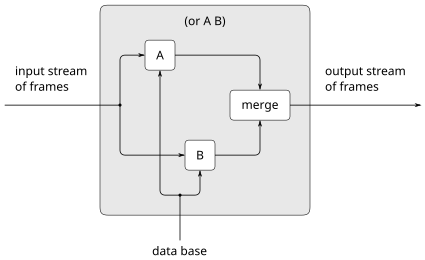
\includegraphics[width=107mm]{assets/figures/chapter_4/figure_4.6.pdf}
\end{imageFigure}

\link{Figure 4.6} shows the analogous method for computing the
\code{or} of two
queries as a parallel combination of the two component queries.  The input
stream of frames is extended separately by each query.  The two resulting
streams are then merged to produce the final output stream.

Even from this high-level description, it is apparent that the processing of
compound queries can be slow.  For example, since a query may produce more than
one output frame for each input frame, and each query in an \code{and} gets its
input frames from the previous query, an \code{and} query could, in the worst
case, have to perform a number of matches that is exponential in the number of
queries (see \link{Exercise 4.76}).\footnote{But this kind of exponential
explosion is not common in \code{and} queries because the added conditions tend
to reduce rather than expand the number of frames produced.} Though systems for
handling only simple queries are quite practical, dealing with complex queries
is extremely difficult.\footnote{There is a large literature on
data-base-management systems that is concerned with how to handle complex
queries efficiently.}

From the stream-of-frames viewpoint, the \code{not} of some query acts as a
filter that removes all frames for which the query can be satisfied.  For
instance, given the pattern

\begin{codeBlock}
(not (job ?x (computer programmer)))
\end{codeBlock}

\noindent
we attempt, for each frame in the input stream, to produce extension frames
that satisfy \code{(job ?x (computer programmer))}.  We remove from the input
stream all frames for which such extensions exist.  The result is a stream
consisting of only those frames in which the binding for \code{?x} does not
satisfy \code{(job ?x (computer programmer))}.  For example, in processing the
query

\begin{codeBlock}
(and (supervisor ?x ?y)
     (not (job ?x (computer programmer))))
\end{codeBlock}

\noindent
the first clause will generate frames with bindings for \code{?x} and
\code{?y}.  The \code{not} clause will then filter these by removing all frames
in which the binding for \code{?x} satisfies the restriction that \code{?x} is
a computer programmer.\footnote{There is a subtle difference between this
filter implementation of \code{not} and the usual meaning of \code{not} in
mathematical logic.  See \link{Section 4.4.3}.}

The \code{lisp\-/value} special form is implemented as a similar filter on frame
streams.  We use each frame in the stream to instantiate any variables in the
pattern, then apply the Lisp predicate.  We remove from the input stream all
frames for which the predicate fails.

\subsubsection*{Unification}

In order to handle rules in the query language, we must be able to find the
rules whose conclusions match a given query pattern.  Rule conclusions are like
assertions except that they can contain variables, so we will need a
generalization of pattern matching---called \newterm{unification}---in which
both the ``pattern'' and the ``datum'' may contain variables.

A unifier takes two patterns, each containing constants and variables, and
determines whether it is possible to assign values to the variables that will
make the two patterns equal.  If so, it returns a frame containing these
bindings.  For example, unifying \code{(?x a ?y)} and \code{(?y ?z a)} will
specify a frame in which \code{?x}, \code{?y}, and \code{?z} must all be bound
to \code{a}.  On the other hand, unifying \code{(?x ?y a)} and \code{(?x b ?y)}
will fail, because there is no value for \code{?y} that can make the two
patterns equal.  (For the second elements of the patterns to be equal,
\code{?y} would have to be \code{b}; however, for the third elements to be
equal, \code{?y} would have to be \code{a}.)  The unifier used in the query
system, like the pattern matcher, takes a frame as input and performs
unifications that are consistent with this frame.

The unification algorithm is the most technically difficult part of the query
system.  With complex patterns, performing unification may seem to require
deduction.  To unify \code{(?x ?x)} and \code{((a ?y c) (a b ?z))}, for
example, the algorithm must infer that \code{?x} should be \code{(a b c)},
\code{?y} should be \code{b}, and \code{?z} should be \code{c}.  We may think
of this process as solving a set of equations among the pattern components.  In
general, these are simultaneous equations, which may require substantial
manipulation to solve.\footnote{In one-sided pattern matching, all the
equations that contain pattern variables are explicit and already solved for
the unknown (the pattern variable).} For example, unifying \code{(?x ?x)} and
\code{((a ?y c) (a b ?z))} may be thought of as specifying the simultaneous
equations

\begin{codeBlock}
?x  =  (a ?y c)
?x  =  (a b ?z)
\end{codeBlock}

\noindent
These equations imply that

\begin{codeBlock}
(a ?y c)  =  (a b ?z)
\end{codeBlock}

\noindent
which in turn implies that

\begin{codeBlock}
 a  =  a,
?y  =  b,
 c  =  ?z,
\end{codeBlock}

\noindent
and hence that

\begin{codeBlock}
?x  =  (a b c)
\end{codeBlock}

\noindent
In a successful pattern match, all pattern variables become bound, and the
values to which they are bound contain only constants.  This is also true of
all the examples of unification we have seen so far.  In general, however, a
successful unification may not completely determine the variable values; some
variables may remain unbound and others may be bound to values that contain
variables.

Consider the unification of \code{(?x a)} and \code{((b ?y) ?z)}.  We can
deduce that \code{?x = (b ?y)} and \code{a = ?z}, but we cannot further solve
for \code{?x} or \code{?y}.  The unification doesn't fail, since it is
certainly possible to make the two patterns equal by assigning values to
\code{?x} and \code{?y}.  Since this match in no way restricts the values
\code{?y} can take on, no binding for \code{?y} is put into the result frame.
The match does, however, restrict the value of \code{?x}.  Whatever value
\code{?y} has, \code{?x} must be \code{(b ?y)}.  A binding of \code{?x} to the
pattern \code{(b ?y)} is thus put into the frame.  If a value for \code{?y} is
later determined and added to the frame (by a pattern match or unification that
is required to be consistent with this frame), the previously bound \code{?x}
will refer to this value.\footnote{Another way to think of unification is that
it generates the most general pattern that is a specialization of the two input
patterns.  That is, the unification of \code{(?x a)} and \code{((b ?y) ?z)} is
\code{((b ?y) a)}, and the unification of \code{(?x a ?y)} and \code{(?y ?z
a)}, discussed above, is \code{(a a a)}.  For our implementation, it is more
convenient to think of the result of unification as a frame rather than a
pattern.}

\subsubsection*{Applying rules}

Unification is the key to the component of the query system that makes
inferences from rules. To see how this is accomplished, consider processing a
query that involves applying a rule, such as

\begin{codeBlock}
(lives-near ?x (Hacker Alyssa P))
\end{codeBlock}

\noindent
To process this query, we first use the ordinary pattern-match procedure
described above to see if there are any assertions in the data base that match
this pattern.  (There will not be any in this case, since our data base
includes no direct assertions about who lives near whom.)  The next step is to
attempt to unify the query pattern with the conclusion of each rule.  We find
that the pattern unifies with the conclusion of the rule

\begin{codeBlock}
(rule (lives-near ?person-1 ?person-2)
      (and (address ?person-1 (?town . ?rest-1))
           (address ?person-2 (?town . ?rest-2))
           (not (same ?person-1 ?person-2))))
\end{codeBlock}

\noindent
resulting in a frame specifying that \code{?person\-/2} is bound to \code{(Hacker
Alyssa P)} and that \code{?x} should be bound to (have the same value as)
\code{?person\-/1}.  Now, relative to this frame, we evaluate the compound query
given by the body of the rule.  Successful matches will extend this frame by
providing a binding for \code{?person\-/1}, and consequently a value for
\code{?x}, which we can use to instantiate the original query pattern.

In general, the query evaluator uses the following method to apply a rule when
trying to establish a query pattern in a frame that specifies bindings for some
of the pattern variables:

\begin{itemize}

\item
Unify the query with the conclusion of the rule to form, if successful, an
extension of the original frame.

\item
Relative to the extended frame, evaluate the query formed by the body of the
rule.

\end{itemize}

\noindent
Notice how similar this is to the method for applying a procedure in the
\code{eval}/\code{apply} evaluator for Lisp:

\begin{itemize}

\item
Bind the procedure's parameters to its arguments to form a frame that extends
the original procedure environment.

\item
Relative to the extended environment, evaluate the expression formed by the
body of the procedure.

\end{itemize}

\noindent
The similarity between the two evaluators should come as no surprise.  Just as
procedure definitions are the means of abstraction in Lisp, rule definitions
are the means of abstraction in the query language.  In each case, we unwind
the abstraction by creating appropriate bindings and evaluating the rule or
procedure body relative to these.

\subsubsection*{Simple queries}

We saw earlier in this section how to evaluate simple queries in the absence of
rules.  Now that we have seen how to apply rules, we can describe how to
evaluate simple queries by using both rules and assertions.

Given the query pattern and a stream of frames, we produce, for each frame in
the input stream, two streams:

\begin{itemize}

\item
a stream of extended frames obtained by matching the pattern against all
assertions in the data base (using the pattern matcher), and

\item
a stream of extended frames obtained by applying all possible rules (using the
unifier).\footnote{Since unification is a generalization of matching, we could
simplify the system by using the unifier to produce both streams.  Treating the
easy case with the simple matcher, however, illustrates how matching (as
opposed to full-blown unification) can be useful in its own right.}

\end{itemize}

\noindent
Appending these two streams produces a stream that consists of all the ways
that the given pattern can be satisfied consistent with the original frame.
These streams (one for each frame in the input stream) are now all combined to
form one large stream, which therefore consists of all the ways that any of the
frames in the original input stream can be extended to produce a match with the
given pattern.

\subsubsection*{The query evaluator and the driver loop}

Despite the complexity of the underlying matching operations, the system is
organized much like an evaluator for any language.  The procedure that
coordinates the matching operations is called \code{qeval}, and it plays a role
analogous to that of the \code{eval} procedure for Lisp.  \code{qeval} takes as
inputs a query and a stream of frames.  Its output is a stream of frames,
corresponding to successful matches to the query pattern, that extend some
frame in the input stream, as indicated in \link{Figure 4.4}.  Like \code{eval},
\code{qeval} classifies the different types of expressions (queries) and
dispatches to an appropriate procedure for each.  There is a procedure for each
special form (\code{and}, \code{or}, \code{not}, and \code{lisp\-/value}) and one
for simple queries.

The driver loop, which is analogous to the \code{driver\-/loop} procedure for the
other evaluators in this chapter, reads queries from the terminal.  For each
query, it calls \code{qeval} with the query and a stream that consists of a
single empty frame.  This will produce the stream of all possible matches (all
possible extensions to the empty frame).  For each frame in the resulting
stream, it instantiates the original query using the values of the variables
found in the frame.  This stream of instantiated queries is then
printed.\footnote{The reason we use streams (rather than lists) of frames is
that the recursive application of rules can generate infinite numbers of values
that satisfy a query.  The delayed evaluation embodied in streams is crucial
here: The system will print responses one by one as they are generated,
regardless of whether there are a finite or infinite number of responses.}

The driver also checks for the special command \code{assert!}, which signals
that the input is not a query but rather an assertion or rule to be added to
the data base.  For instance,

\begin{codeBlock}
(assert! (job (Bitdiddle Ben)
              (computer wizard)))
(assert! (rule (wheel ?person)
               (and (supervisor ?middle-manager ?person)
                    (supervisor ?x ?middle-manager))))
\end{codeBlock}


\subsection{Is Logic Programming Mathematical Logic?}
\label{Section 4.4.3}

The means of combination used in the query language may at first seem identical
to the operations \code{and}, \code{or}, and \code{not} of mathematical logic,
and the application of query-language rules is in fact accomplished through a
legitimate method of inference.\footnote{That a particular method of inference
is legitimate is not a trivial assertion.  One must prove that if one starts
with true premises, only true conclusions can be derived.  The method of
inference represented by rule applications is \newterm{modus ponens}, the
familiar method of inference that says that if \( A \) is true and \emph{A
implies B} is true, then we may conclude that \( B \) is true.} This
identification of the query language with mathematical logic is not really
valid, though, because the query language provides a \newterm{control
structure} that interprets the logical statements procedurally.  We can often
take advantage of this control structure.  For example, to find all of the
supervisors of programmers we could formulate a query in either of two
logically equivalent forms:

\begin{codeBlock}
(and (job ?x (computer programmer)) (supervisor ?x ?y))
\end{codeBlock}

\noindent
or

\begin{codeBlock}
(and (supervisor ?x ?y) (job ?x (computer programmer)))
\end{codeBlock}

\noindent
If a company has many more supervisors than programmers (the usual case), it is
better to use the first form rather than the second because the data base must
be scanned for each intermediate result (frame) produced by the first clause of
the \code{and}.

The aim of logic programming is to provide the programmer with techniques for
decomposing a computational problem into two separate problems: ``what'' is to
be computed, and ``how'' this should be computed.  This is accomplished by
selecting a subset of the statements of mathematical logic that is powerful
enough to be able to describe anything one might want to compute, yet weak
enough to have a controllable procedural interpretation.  The intention here is
that, on the one hand, a program specified in a logic programming language
should be an effective program that can be carried out by a computer.  Control
(``how'' to compute) is effected by using the order of evaluation of the
language.  We should be able to arrange the order of clauses and the order of
subgoals within each clause so that the computation is done in an order deemed
to be effective and efficient.  At the same time, we should be able to view the
result of the computation (``what'' to compute) as a simple consequence of the
laws of logic.

Our query language can be regarded as just such a procedurally interpretable
subset of mathematical logic.  An assertion represents a simple fact (an atomic
proposition).  A rule represents the implication that the rule conclusion holds
for those cases where the rule body holds.  A rule has a natural procedural
interpretation: To establish the conclusion of the rule, establish the body of
the rule.  Rules, therefore, specify computations.  However, because rules can
also be regarded as statements of mathematical logic, we can justify any
``inference'' accomplished by a logic program by asserting that the same result
could be obtained by working entirely within mathematical logic.\footnote{We
must qualify this statement by agreeing that, in speaking of the ``inference''
accomplished by a logic program, we assume that the computation terminates.
Unfortunately, even this qualified statement is false for our implementation of
the query language (and also false for programs in Prolog and most other
current logic programming languages) because of our use of \code{not} and
\code{lisp\-/value}.  As we will describe below, the \code{not} implemented in
the query language is not always consistent with the \code{not} of mathematical
logic, and \code{lisp\-/value} introduces additional complications.  We could
implement a language consistent with mathematical logic by simply removing
\code{not} and \code{lisp\-/value} from the language and agreeing to write
programs using only simple queries, \code{and}, and \code{or}.  However, this
would greatly restrict the expressive power of the language.  One of the major
concerns of research in logic programming is to find ways to achieve more
consistency with mathematical logic without unduly sacrificing expressive
power.}

\subsubsection*{Infinite loops}

A consequence of the procedural interpretation of logic programs is that it is
possible to construct hopelessly inefficient programs for solving certain
problems.  An extreme case of inefficiency occurs when the system falls into
infinite loops in making deductions.  As a simple example, suppose we are
setting up a data base of famous marriages, including

\begin{codeBlock}
(assert! (married Minnie Mickey))
\end{codeBlock}

\noindent
If we now ask

\begin{codeBlock}
(married Mickey ?who)
\end{codeBlock}

\noindent
we will get no response, because the system doesn't know that if \( A \) is
married to \( B \), then \( B \) is married to \( A \).  So we assert the rule

\begin{codeBlock}
(assert! (rule (married ?x ?y) (married ?y ?x)))
\end{codeBlock}

\noindent
and again query

\begin{codeBlock}
(married Mickey ?who)
\end{codeBlock}

\noindent
Unfortunately, this will drive the system into an infinite loop, as follows:

\begin{itemize}

\item
The system finds that the \code{married} rule is applicable; that is, the rule
conclusion \code{(married ?x ?y)} successfully unifies with the query pattern
\code{(married Mickey ?who)} to produce a frame in which \code{?x} is bound to
\code{Mickey} and \code{?y} is bound to \code{?who}.  So the interpreter
proceeds to evaluate the rule body \code{(married ?y ?x)} in this frame---in
effect, to process the query \code{(married ?who Mickey)}.

\item
One answer appears directly as an assertion in the data base: \code{(married
Minnie Mickey)}.

\item
The \code{married} rule is also applicable, so the interpreter again evaluates
the rule body, which this time is equivalent to \code{(married Mickey ?who)}.

\end{itemize}

\noindent
The system is now in an infinite loop.  Indeed, whether the system will find
the simple answer \code{(married Minnie Mickey)} before it goes into the loop
depends on implementation details concerning the order in which the system
checks the items in the data base.  This is a very simple example of the kinds
of loops that can occur.  Collections of interrelated rules can lead to loops
that are much harder to anticipate, and the appearance of a loop can depend on
the order of clauses in an \code{and} (see \link{Exercise 4.64}) or on low-level
details concerning the order in which the system processes
queries.\footnote{This is not a problem of the logic but one of the procedural
interpretation of the logic provided by our interpreter.  We could write an
interpreter that would not fall into a loop here.  For example, we could
enumerate all the proofs derivable from our assertions and our rules in a
breadth-first rather than a depth-first order.  However, such a system makes it
more difficult to take advantage of the order of deductions in our programs.
One attempt to build sophisticated control into such a program is described in
\link{deKleer et al. 1977}.  Another technique, which does not lead to such serious
control problems, is to put in special knowledge, such as detectors for
particular kinds of loops (\link{Exercise 4.67}).  However, there can be no
general scheme for reliably preventing a system from going down infinite paths
in performing deductions.  Imagine a diabolical rule of the form ``To show
\( P(x) \) is true, show that \( P(f(x)) \) is true,'' for some
suitably chosen function \( f \).}

\subsubsection*{Problems with \code{not}}

Another quirk in the query system concerns \code{not}.  Given the data base of
\link{Section 4.4.1}, consider the following two queries:

\begin{codeBlock}
(and (supervisor ?x ?y)
     (not (job ?x (computer programmer))))
(and (not (job ?x (computer programmer)))
     (supervisor ?x ?y))
\end{codeBlock}

\noindent
These two queries do not produce the same result.  The first query begins by
finding all entries in the data base that match \code{(supervisor ?x ?y)}, and
then filters the resulting frames by removing the ones in which the value of
\code{?x} satisfies \code{(job ?x (computer programmer))}.  The second query
begins by filtering the incoming frames to remove those that can satisfy
\code{(job ?x (computer programmer))}.  Since the only incoming frame is empty,
it checks the data base to see if there are any patterns that satisfy
\code{(job ?x (computer programmer))}.  Since there generally are entries of
this form, the \code{not} clause filters out the empty frame and returns an
empty stream of frames.  Consequently, the entire compound query returns an
empty stream.

The trouble is that our implementation of \code{not} really is meant to serve
as a filter on values for the variables.  If a \code{not} clause is processed
with a frame in which some of the variables remain unbound (as does \code{?x}
in the example above), the system will produce unexpected results. Similar
problems occur with the use of \code{lisp\-/value}---the Lisp predicate can't
work if some of its arguments are unbound.  See \link{Exercise 4.77}.

There is also a much more serious way in which the \code{not} of the query
language differs from the \code{not} of mathematical logic.  In logic, we
interpret the statement ``not \( P \)'' to mean that \( P \) is not true.  In the
query system, however, ``not \( P \)'' means that \( P \) is not deducible from the
knowledge in the data base.  For example, given the personnel data base of
\link{Section 4.4.1}, the system would happily deduce all sorts of \code{not}
statements, such as that Ben Bitdiddle is not a baseball fan, that it is not
raining outside, and that 2 + 2 is not 4.\footnote{Consider the query
\code{(not (baseball\-/fan (Bitdiddle Ben)))}.  The system finds that
\code{(baseball\-/fan (Bitdiddle Ben))} is not in the data base, so the empty
frame does not satisfy the pattern and is not filtered out of the initial
stream of frames.  The result of the query is thus the empty frame, which is
used to instantiate the input query to produce \code{(not (baseball\-/fan
(Bitdiddle Ben)))}.} In other words, the \code{not} of logic programming
languages reflects the so-called \newterm{closed world assumption} that all
relevant information has been included in the data base.\footnote{A discussion
and justification of this treatment of \code{not} can be found in the article
by \link{Clark (1978)}.}

\begin{exerciseGroup}
\exerciseHeading{\phantomsection\label{Exercise 4.64}Exercise 4.64:} Louis Reasoner mistakenly deletes
the \code{outranked\-/by} rule (\link{Section 4.4.1}) from the data base.  When he
realizes this, he quickly reinstalls it.  Unfortunately, he makes a slight
change in the rule, and types it in as

\begin{codeBlock}
(rule (outranked-by ?staff-person ?boss)
      (or (supervisor ?staff-person ?boss)
          (and (outranked-by ?middle-manager ?boss)
               (supervisor ?staff-person
                           ?middle-manager))))
\end{codeBlock}

Just after Louis types this information into the system, DeWitt Aull comes by
to find out who outranks Ben Bitdiddle. He issues the query

\begin{codeBlock}
(outranked-by (Bitdiddle Ben) ?who)
\end{codeBlock}

After answering, the system goes into an infinite loop.  Explain why.

\exerciseHeading{\phantomsection\label{Exercise 4.65}Exercise 4.65:} Cy D. Fect, looking forward to
the day when he will rise in the organization, gives a query to find all the
wheels (using the \code{wheel} rule of \link{Section 4.4.1}):

\begin{codeBlock}
(wheel ?who)
\end{codeBlock}

To his surprise, the system responds

\begin{codeBlock}
~\textit{;;; Query results:}~
(wheel (Warbucks Oliver))
(wheel (Bitdiddle Ben))
(wheel (Warbucks Oliver))
(wheel (Warbucks Oliver))
(wheel (Warbucks Oliver))
\end{codeBlock}

Why is Oliver Warbucks listed four times?

\exerciseHeading{\phantomsection\label{Exercise 4.66}Exercise 4.66:} Ben has been generalizing the
query system to provide statistics about the company.  For example, to find the
total salaries of all the computer programmers one will be able to say

\begin{codeBlock}
(sum ?amount (and (job ?x (computer programmer))
                  (salary ?x ?amount)))
\end{codeBlock}

In general, Ben's new system allows expressions of the form

\begin{codeBlock}
(accumulation-function ~\(\langle \)~~\var{variable}~~\(\rangle \)~ ~\(\langle \)~~\var{query pattern}~~\(\rangle \)~)
\end{codeBlock}

\noindent
where \code{accumulation\-/function} can be things like \code{sum},
\code{average}, or \code{maximum}.  Ben reasons that it should be a cinch to
implement this.  He will simply feed the query pattern to \code{qeval}.  This
will produce a stream of frames.  He will then pass this stream through a
mapping function that extracts the value of the designated variable from each
frame in the stream and feed the resulting stream of values to the accumulation
function.  Just as Ben completes the implementation and is about to try it out,
Cy walks by, still puzzling over the \code{wheel} query result in
\link{Exercise 4.65}.  When Cy shows Ben the system's response, Ben groans,
``Oh, no, my simple accumulation scheme won't work!''

What has Ben just realized?  Outline a method he can use to salvage the
situation.

\exerciseHeading{\phantomsection\label{Exercise 4.67}Exercise 4.67:} Devise a way to install a loop
detector in the query system so as to avoid the kinds of simple loops
illustrated in the text and in \link{Exercise 4.64}.
The general idea is that
the system should maintain some sort of history of its current chain of
deductions and should not begin processing a query that it is already working
on.  Describe what kind of information (patterns and frames) is included in
this history, and how the check should be made.  (After you study the details
of the query-system implementation in \link{Section 4.4.4}, you may want to
modify the system to include your loop detector.)

\exerciseHeading{\phantomsection\label{Exercise 4.68}Exercise 4.68:} Define rules to implement the
\code{reverse} operation of \link{Exercise 2.18}, which returns a list
containing the same elements as a given list in reverse order.  (Hint: Use
\code{append\-/to\-/form}.)  Can your rules answer both \code{(reverse (1 2 3) ?x)}
and \code{(reverse ?x (1 2 3))} ?

\exerciseHeading{\phantomsection\label{Exercise 4.69}Exercise 4.69:} Beginning with the data base and
the rules you formulated in \link{Exercise 4.63}, devise a rule for adding
``greats'' to a grandson relationship. This should enable the system to deduce
that Irad is the great-grandson of Adam, or that Jabal and Jubal are the
great-great-great-great-great-grandsons of Adam.  (Hint: Represent the fact
about Irad, for example, as \code{((great grandson) Adam Irad)}.  Write rules
that determine if a list ends in the word \code{grandson}.  Use this to express
a rule that allows one to derive the relationship \code{((great .  ?rel) ?x
?y)}, where \code{?rel} is a list ending in \code{grandson}.)  Check your rules
on queries such as \code{((great grandson) ?g ?ggs)} and \code{(?relationship
Adam Irad)}.
\end{exerciseGroup}

\subsection{Implementing the Query System}
\label{Section 4.4.4}

\link{Section 4.4.2} described how the query system works. Now we fill in the
details by presenting a complete implementation of the system.



\subsubsection{The Driver Loop and Instantiation}
\label{Section 4.4.4.1}

The driver loop for the query system repeatedly reads input expressions.  If
the expression is a rule or assertion to be added to the data base, then the
information is added.  Otherwise the expression is assumed to be a query.  The
driver passes this query to the evaluator \code{qeval} together with an initial
frame stream consisting of a single empty frame.  The result of the evaluation
is a stream of frames generated by satisfying the query with variable values
found in the data base.  These frames are used to form a new stream consisting
of copies of the original query in which the variables are instantiated with
values supplied by the stream of frames, and this final stream is printed at
the terminal:

\begin{codeBlock}
(define input-prompt  ";;; Query input:")
(define output-prompt ";;; Query results:")

(define (query-driver-loop)
  (prompt-for-input input-prompt)
  (let ((q (query-syntax-process (read))))
    (cond ((assertion-to-be-added? q)
           (add-rule-or-assertion! (add-assertion-body q))
           (newline)
           (display "Assertion added to data base.")
           (query-driver-loop))
          (else
           (newline)
           (display output-prompt)
           (display-stream
            (stream-map
             (lambda (frame)
               (instantiate
                q
                frame
                (lambda (v f)
                  (contract-question-mark v))))
             (qeval q (singleton-stream '()))))
           (query-driver-loop)))))
\end{codeBlock}

\noindent
Here, as in the other evaluators in this chapter, we use an abstract syntax for
the expressions of the query language.  The implementation of the expression
syntax, including the predicate \code{assertion\-/to\-/be\-/added?} and the selector
\code{add\-/assertion\-/body}, is given in \link{Section 4.4.4.7}.
\code{add\-/rule\-/or\-/assertion!} is defined in \link{Section 4.4.4.5}.

Before doing any processing on an input expression, the driver loop transforms
it syntactically into a form that makes the processing more efficient.  This
involves changing the representation of pattern variables.  When the query is
instantiated, any variables that remain unbound are transformed back to the
input representation before being printed.  These transformations are performed
by the two procedures \code{query\-/syntax\-/process} and
\code{contract\-/question\-/mark} (\link{Section 4.4.4.7}).

To instantiate an expression, we copy it, replacing any variables in the
expression by their values in a given frame.  The values are themselves
instantiated, since they could contain variables (for example, if \code{?x} in
\code{exp} is bound to \code{?y} as the result of unification and \code{?y} is
in turn bound to 5).  The action to take if a variable cannot be instantiated
is given by a procedural argument to \code{instantiate}.

\begin{codeBlock}
(define (instantiate exp frame unbound-var-handler)
  (define (copy exp)
    (cond ((var? exp)
           (let ((binding (binding-in-frame exp frame)))
             (if binding
                 (copy (binding-value binding))
                 (unbound-var-handler exp frame))))
          ((pair? exp)
           (cons (copy (car exp)) (copy (cdr exp))))
          (else exp)))
  (copy exp))
\end{codeBlock}

\noindent
The procedures that manipulate bindings are defined in \link{Section 4.4.4.8}.

\subsubsection{The Evaluator}
\label{Section 4.4.4.2}

The \code{qeval} procedure, called by the \code{query\-/driver\-/loop}, is the
basic evaluator of the query system.  It takes as inputs a query and a stream
of frames, and it returns a stream of extended frames.  It identifies special
forms by a data-directed dispatch using \code{get} and \code{put}, just as we
did in implementing generic operations in \link{Chapter 2}.  Any query that is
not identified as a special form is assumed to be a simple query, to be
processed by \code{simple\-/query}.

\begin{codeBlock}
(define (qeval query frame-stream)
  (let ((qproc (get (type query) 'qeval)))
    (if qproc
        (qproc (contents query) frame-stream)
        (simple-query query frame-stream))))
\end{codeBlock}

\noindent
\code{type} and \code{contents}, defined in \link{Section 4.4.4.7}, implement
the abstract syntax of the special forms.

\subsubsection*{Simple queries}

The \code{simple\-/query} procedure handles simple queries.  It takes as
arguments a simple query (a pattern) together with a stream of frames, and it
returns the stream formed by extending each frame by all data-base matches of
the query.

\begin{codeBlock}
(define (simple-query query-pattern frame-stream)
  (stream-flatmap
   (lambda (frame)
     (stream-append-delayed
      (find-assertions query-pattern frame)
      (delay (apply-rules query-pattern frame))))
   frame-stream))
\end{codeBlock}

\noindent
For each frame in the input stream, we use \code{find\-/assertions}
(\link{Section 4.4.4.3}) to match the pattern against all assertions in the data base,
producing a stream of extended frames, and we use \code{apply\-/rules}
(\link{Section 4.4.4.4}) to apply all possible rules, producing another stream of
extended frames.  These two streams are combined (using
\code{stream\-/append\-/delayed}, \link{Section 4.4.4.6}) to make a stream of all
the ways that the given pattern can be satisfied consistent with the original
frame (see \link{Exercise 4.71}).  The streams for the individual input frames
are combined using \code{stream\-/flatmap} (\link{Section 4.4.4.6}) to form one
large stream of all the ways that any of the frames in the original input
stream can be extended to produce a match with the given pattern.

\subsubsection*{Compound queries}

\code{and} queries are handled as illustrated in \link{Figure 4.5} by the
\code{conjoin} procedure.  \code{conjoin} takes as inputs the conjuncts and the
frame stream and returns the stream of extended frames.  First, \code{conjoin}
processes the stream of frames to find the stream of all possible frame
extensions that satisfy the first query in the conjunction.  Then, using this
as the new frame stream, it recursively applies \code{conjoin} to the rest of
the queries.

\begin{codeBlock}
(define (conjoin conjuncts frame-stream)
  (if (empty-conjunction? conjuncts)
      frame-stream
      (conjoin (rest-conjuncts conjuncts)
               (qeval (first-conjunct conjuncts) frame-stream))))
\end{codeBlock}

\noindent
The expression

\begin{codeBlock}
(put 'and 'qeval conjoin)
\end{codeBlock}

\noindent
sets up \code{qeval} to dispatch to \code{conjoin} when an \code{and} form is
encountered.

\code{or} queries are handled similarly, as shown in \link{Figure 4.6}.  The
output streams for the various disjuncts of the \code{or} are computed
separately and merged using the \code{interleave\-/delayed} procedure from
\link{Section 4.4.4.6}.  (See \link{Exercise 4.71} and \link{Exercise 4.72}.)

\begin{codeBlock}
(define (disjoin disjuncts frame-stream)
  (if (empty-disjunction? disjuncts)
      the-empty-stream
      (interleave-delayed
       (qeval (first-disjunct disjuncts) frame-stream)
       (delay (disjoin (rest-disjuncts disjuncts) frame-stream)))))
(put 'or 'qeval disjoin)
\end{codeBlock}

\noindent
The predicates and selectors for the syntax of conjuncts and disjuncts are
given in \link{Section 4.4.4.7}.

\subsubsection*{Filters}

\code{not} is handled by the method outlined in \link{Section 4.4.2}.  We
attempt to extend each frame in the input stream to satisfy the query being
negated, and we include a given frame in the output stream only if it cannot be
extended.

\begin{codeBlock}
(define (negate operands frame-stream)
  (stream-flatmap
   (lambda (frame)
     (if (stream-null?
          (qeval (negated-query operands)
                 (singleton-stream frame)))
         (singleton-stream frame)
         the-empty-stream))
   frame-stream))
(put 'not 'qeval negate)
\end{codeBlock}

\noindent
\code{lisp\-/value} is a filter similar to \code{not}.  Each frame in the stream
is used to instantiate the variables in the pattern, the indicated predicate is
applied, and the frames for which the predicate returns false are filtered out
of the input stream.  An error results if there are unbound pattern variables.

\begin{codeBlock}
(define (lisp-value call frame-stream)
  (stream-flatmap
   (lambda (frame)
     (if (execute
          (instantiate
           call
           frame
           (lambda (v f)
             (error "Unknown pat var: LISP-VALUE" v))))
         (singleton-stream frame)
         the-empty-stream))
   frame-stream))
(put 'lisp-value 'qeval lisp-value)
\end{codeBlock}

\noindent
\code{execute}, which applies the predicate to the arguments, must \code{eval}
the predicate expression to get the procedure to apply.  However, it must not
evaluate the arguments, since they are already the actual arguments, not
expressions whose evaluation (in Lisp) will produce the arguments.  Note that
\code{execute} is implemented using \code{eval} and \code{apply} from the
underlying Lisp system.

\begin{codeBlock}
(define (execute exp)
  (apply (eval (predicate exp) user-initial-environment)
         (args exp)))
\end{codeBlock}

\noindent
The \code{always\-/true} special form provides for a query that is always
satisfied.  It ignores its contents (normally empty) and simply passes through
all the frames in the input stream.  \code{always\-/true} is used by the
\code{rule\-/body} selector (\link{Section 4.4.4.7}) to provide bodies for rules
that were defined without bodies (that is, rules whose conclusions are always
satisfied).

\begin{codeBlock}
(define (always-true ignore frame-stream) frame-stream)
(put 'always-true 'qeval always-true)
\end{codeBlock}

\noindent
The selectors that define the syntax of \code{not} and \code{lisp\-/value} are
given in \link{Section 4.4.4.7}.

\subsubsection{Finding Assertions by Pattern Matching}
\label{Section 4.4.4.3}

\code{find\-/assertions}, called by \code{simple\-/query} (\link{Section 4.4.4.2}),
takes as input a pattern and a frame.  It returns a stream of frames, each
extending the given one by a data-base match of the given pattern.  It uses
\code{fetch\-/assertions} (\link{Section 4.4.4.5}) to get a stream of all the
assertions in the data base that should be checked for a match against the
pattern and the frame.  The reason for \code{fetch\-/assertions} here is that we
can often apply simple tests that will eliminate many of the entries in the
data base from the pool of candidates for a successful match.  The system would
still work if we eliminated \code{fetch\-/assertions} and simply checked a stream
of all assertions in the data base, but the computation would be less efficient
because we would need to make many more calls to the matcher.

\begin{codeBlock}
(define (find-assertions pattern frame)
  (stream-flatmap
   (lambda (datum) (check-an-assertion datum pattern frame))
   (fetch-assertions pattern frame)))
\end{codeBlock}

\noindent
\code{check\-/an\-/assertion} takes as arguments a pattern, a data object
(assertion), and a frame and returns either a one-element stream containing the
extended frame or \code{the\-/empty\-/stream} if the match fails.

\begin{codeBlock}
(define (check-an-assertion assertion query-pat query-frame)
  (let ((match-result
         (pattern-match query-pat assertion query-frame)))
    (if (eq? match-result 'failed)
        the-empty-stream
        (singleton-stream match-result))))
\end{codeBlock}

\noindent
The basic pattern matcher returns either the symbol \code{failed} or an
extension of the given frame.  The basic idea of the matcher is to check the
pattern against the data, element by element, accumulating bindings for the
pattern variables.  If the pattern and the data object are the same, the match
succeeds and we return the frame of bindings accumulated so far.  Otherwise, if
the pattern is a variable we extend the current frame by binding the variable
to the data, so long as this is consistent with the bindings already in the
frame.  If the pattern and the data are both pairs, we (recursively) match the
\code{car} of the pattern against the \code{car} of the data to produce a
frame; in this frame we then match the \code{cdr} of the pattern against the
\code{cdr} of the data.  If none of these cases are applicable, the match fails
and we return the symbol \code{failed}.

\begin{codeBlock}
(define (pattern-match pat dat frame)
  (cond ((eq? frame 'failed) 'failed)
        ((equal? pat dat) frame)
        ((var? pat) (extend-if-consistent pat dat frame))
        ((and (pair? pat) (pair? dat))
         (pattern-match
          (cdr pat)
          (cdr dat)
          (pattern-match (car pat) (car dat) frame)))
        (else 'failed)))
\end{codeBlock}

\noindent
Here is the procedure that extends a frame by adding a new binding, if this is
consistent with the bindings already in the frame:

\begin{codeBlock}
(define (extend-if-consistent var dat frame)
  (let ((binding (binding-in-frame var frame)))
    (if binding
        (pattern-match (binding-value binding) dat frame)
        (extend var dat frame))))
\end{codeBlock}

\noindent
If there is no binding for the variable in the frame, we simply add the binding
of the variable to the data.  Otherwise we match, in the frame, the data
against the value of the variable in the frame.  If the stored value contains
only constants, as it must if it was stored during pattern matching by
\code{extend\-/if\-/consistent}, then the match simply tests whether the stored and
new values are the same.  If so, it returns the unmodified frame; if not, it
returns a failure indication.  The stored value may, however, contain pattern
variables if it was stored during unification (see \link{Section 4.4.4.4}).  The
recursive match of the stored pattern against the new data will add or check
bindings for the variables in this pattern.  For example, suppose we have a
frame in which \code{?x} is bound to \code{(f ?y)} and \code{?y} is unbound,
and we wish to augment this frame by a binding of \code{?x} to \code{(f b)}.
We look up \code{?x} and find that it is bound to \code{(f ?y)}.  This leads us
to match \code{(f ?y)} against the proposed new value \code{(f b)} in the same
frame.  Eventually this match extends the frame by adding a binding of
\code{?y} to \code{b}.  \code{?X} remains bound to \code{(f ?y)}.  We never
modify a stored binding and we never store more than one binding for a given
variable.

The procedures used by \code{extend\-/if\-/consistent} to manipulate bindings are
defined in \link{Section 4.4.4.8}.

\subsubsection*{Patterns with dotted tails}

If a pattern contains a dot followed by a pattern variable, the pattern
variable matches the rest of the data list (rather than the next element of the
data list), just as one would expect with the dotted-tail notation described in
\link{Exercise 2.20}.  Although the pattern matcher we have just implemented
doesn't look for dots, it does behave as we want.  This is because the Lisp
\code{read} primitive, which is used by \code{query\-/driver\-/loop} to read the
query and represent it as a list structure, treats dots in a special way.

When \code{read} sees a dot, instead of making the next item be the next
element of a list (the \code{car} of a \code{cons} whose \code{cdr} will be the
rest of the list) it makes the next item be the \code{cdr} of the list
structure.  For example, the list structure produced by \code{read} for the
pattern \code{(computer ?type)} could be constructed by evaluating the
expression \code{(cons 'computer (cons '?type '()))}, and that for
\code{(computer . ?type)} could be constructed by evaluating the expression
\code{(cons 'computer '?type)}.

Thus, as \code{pattern\-/match} recursively compares \code{car}s and \code{cdr}s
of a data list and a pattern that had a dot, it eventually matches the variable
after the dot (which is a \code{cdr} of the pattern) against a sublist of the
data list, binding the variable to that list.  For example, matching the
pattern \code{(computer . ?type)} against \code{(computer programmer trainee)}
will match \code{?type} against the list \code{(programmer trainee)}.

\subsubsection{Rules and Unification}
\label{Section 4.4.4.4}

\code{apply\-/rules} is the rule analog of \code{find\-/assertions}
(\link{Section 4.4.4.3}).  It takes as input a pattern and a frame, and it forms a stream
of extension frames by applying rules from the data base.
\code{stream\-/flatmap} maps \code{apply\-/a\-/rule} down the stream of possibly
applicable rules (selected by \code{fetch\-/rules}, \link{Section 4.4.4.5}) and
combines the resulting streams of frames.

\begin{codeBlock}
(define (apply-rules pattern frame)
  (stream-flatmap (lambda (rule)
                    (apply-a-rule rule pattern frame))
                  (fetch-rules pattern frame)))
\end{codeBlock}

\noindent
\code{apply\-/a\-/rule} applies rules using the method outlined in
\link{Section 4.4.2}.  It first augments its argument frame by unifying the rule
conclusion with the pattern in the given frame.  If this succeeds, it evaluates
the rule body in this new frame.

Before any of this happens, however, the program renames all the variables in
the rule with unique new names.  The reason for this is to prevent the
variables for different rule applications from becoming confused with each
other.  For instance, if two rules both use a variable named \code{?x}, then
each one may add a binding for \code{?x} to the frame when it is applied.
These two \code{?x}'s have nothing to do with each other, and we should not be
fooled into thinking that the two bindings must be consistent.  Rather than
rename variables, we could devise a more clever environment structure; however,
the renaming approach we have chosen here is the most straightforward, even if
not the most efficient.  (See \link{Exercise 4.79}.)  Here is the
\code{apply\-/a\-/rule} procedure:

\begin{codeBlock}
(define (apply-a-rule rule query-pattern query-frame)
  (let ((clean-rule (rename-variables-in rule)))
    (let ((unify-result (unify-match query-pattern
                                     (conclusion clean-rule)
                                     query-frame)))
      (if (eq? unify-result 'failed)
          the-empty-stream
          (qeval (rule-body clean-rule)
                 (singleton-stream unify-result))))))
\end{codeBlock}

\noindent
The selectors \code{rule\-/body} and \code{conclusion} that extract parts of a
rule are defined in \link{Section 4.4.4.7}.

We generate unique variable names by associating a unique identifier (such as a
number) with each rule application and combining this identifier with the
original variable names.  For example, if the rule-application identifier is 7,
we might change each \code{?x} in the rule to \code{?x\-/7} and each \code{?y} in
the rule to \code{?y\-/7}.  (\code{make\-/new\-/variable} and
\code{new\-/rule\-/application\-/id} are included with the syntax procedures in
\link{Section 4.4.4.7}.)

\begin{codeBlock}
(define (rename-variables-in rule)
  (let ((rule-application-id (new-rule-application-id)))
    (define (tree-walk exp)
      (cond ((var? exp)
             (make-new-variable exp rule-application-id))
            ((pair? exp)
             (cons (tree-walk (car exp))
                   (tree-walk (cdr exp))))
            (else exp)))
    (tree-walk rule)))
\end{codeBlock}

\noindent
The unification algorithm is implemented as a procedure that takes as inputs
two patterns and a frame and returns either the extended frame or the symbol
\code{failed}.  The unifier is like the pattern matcher except that it is
symmetrical---variables are allowed on both sides of the match.
\code{unify\-/match} is basically the same as \code{pattern\-/match}, except that
there is extra code (marked ``\code{***}'' below) to handle the case where the
object on the right side of the match is a variable.

\begin{codeBlock}
(define (unify-match p1 p2 frame)
  (cond ((eq? frame 'failed) 'failed)
        ((equal? p1 p2) frame)
        ((var? p1) (extend-if-possible p1 p2 frame))
        ((var? p2) (extend-if-possible p2 p1 frame))  ~\textrm{; ***}~
        ((and (pair? p1) (pair? p2))
         (unify-match (cdr p1)
                      (cdr p2)
                      (unify-match (car p1)
                                   (car p2)
                                   frame)))
        (else 'failed)))
\end{codeBlock}

\noindent
In unification, as in one-sided pattern matching, we want to accept a proposed
extension of the frame only if it is consistent with existing bindings.  The
procedure \code{extend\-/if\-/possible} used in unification is the same as the
\code{extend\-/if\-/consistent} used in pattern matching except for two special
checks, marked ``\code{***}'' in the program below.  In the first case, if the
variable we are trying to match is not bound, but the value we are trying to
match it with is itself a (different) variable, it is necessary to check to see
if the value is bound, and if so, to match its value.  If both parties to the
match are unbound, we may bind either to the other.

The second check deals with attempts to bind a variable to a pattern that
includes that variable.  Such a situation can occur whenever a variable is
repeated in both patterns.  Consider, for example, unifying the two patterns
\code{(?x ?x)} and \code{(?y \( \langle \)\var{expression involving \code{?y}}\( \rangle \))} in a
frame where both \code{?x} and \code{?y} are unbound.  First \code{?x} is
matched against \code{?y}, making a binding of \code{?x} to \code{?y}.  Next,
the same \code{?x} is matched against the given expression involving \code{?y}.
Since \code{?x} is already bound to \code{?y}, this results in matching
\code{?y} against the expression.  If we think of the unifier as finding a set
of values for the pattern variables that make the patterns the same, then these
patterns imply instructions to find a \code{?y} such that \code{?y} is equal to
the expression involving \code{?y}.  There is no general method for solving
such equations, so we reject such bindings; these cases are recognized by the
predicate \code{depends\-/on?}.\footnote{In general, unifying \code{?y} with an
expression involving \code{?y} would require our being able to find a fixed
point of the equation \code{?y} = \( \langle \)\var{expression involving \code{?y}}\( \rangle \).  It
is sometimes possible to syntactically form an expression that appears to be
the solution.  For example, \code{?y} = \code{(f ?y)} seems to have the fixed
point \code{(f (f (f \( \dots \) )))}, which we can produce by beginning with the
expression \code{(f ?y)} and repeatedly substituting \code{(f ?y)} for
\code{?y}.  Unfortunately, not every such equation has a meaningful fixed
point.  The issues that arise here are similar to the issues of manipulating
infinite series in mathematics.  For example, we know that 2 is the solution to
the equation \( y = 1 + y / 2 \).  Beginning with the expression \( 1 + y / 2 \)
and repeatedly substituting \( 1 + y / 2 \) for \( y \) gives

$$ 2 = y = 1 + \frac{y}{2} = 1 + \frac{1}{2}\left(1 + \frac{y}{2}\right) =
	1 + \frac{1}{2} + \frac{y}{4} = \dots , $$

\noindent
which leads to

$$ 2 = 1 + \frac{1}{2} + \frac{1}{4} + \frac{1}{8} + \dots. $$

\noindent
However, if we try the same manipulation beginning with the observation that -1
is the solution to the equation \( y = 1 + 2y \), we obtain

$$ -1 = y = 1 + 2y = 1 + 2(1 + 2y) = 1 + 2 + 4y = \dots, $$

\noindent
which leads to

$$ -1 = 1 + 2 + 4 + 8 + \dots. $$

\noindent
Although the formal manipulations used in deriving these two equations are
identical, the first result is a valid assertion about infinite series but the
second is not.  Similarly, for our unification results, reasoning with an
arbitrary syntactically constructed expression may lead to errors.}  On the
other hand, we do not want to reject attempts to bind a variable to itself.
For example, consider unifying \code{(?x ?x)} and \code{(?y ?y)}.  The second
attempt to bind \code{?x} to \code{?y} matches \code{?y} (the stored value of
\code{?x}) against \code{?y} (the new value of \code{?x}).  This is taken care
of by the \code{equal?}  clause of \code{unify\-/match}.

\begin{codeBlock}
(define (extend-if-possible var val frame)
  (let ((binding (binding-in-frame var frame)))
    (cond (binding
           (unify-match (binding-value binding) val frame))
          ((var? val)                      ~\textrm{; ***}~
           (let ((binding (binding-in-frame val frame)))
             (if binding
                 (unify-match
                  var (binding-value binding) frame)
                 (extend var val frame))))
          ((depends-on? val var frame)     ~\textrm{; ***}~
           'failed)
          (else (extend var val frame)))))
\end{codeBlock}

\noindent
\code{depends\-/on?} is a predicate that tests whether an expression proposed to
be the value of a pattern variable depends on the variable.  This must be done
relative to the current frame because the expression may contain occurrences of
a variable that already has a value that depends on our test variable.  The
structure of \code{depends\-/on?} is a simple recursive tree walk in which we
substitute for the values of variables whenever necessary.

\begin{codeBlock}
(define (depends-on? exp var frame)
  (define (tree-walk e)
    (cond ((var? e)
           (if (equal? var e)
               true
               (let ((b (binding-in-frame e frame)))
                 (if b
                     (tree-walk (binding-value b))
                     false))))
          ((pair? e)
           (or (tree-walk (car e))
               (tree-walk (cdr e))))
          (else false)))
  (tree-walk exp))
\end{codeBlock}

\subsubsection{Maintaining the Data Base}
\label{Section 4.4.4.5}

One important problem in designing logic programming languages is that of
arranging things so that as few irrelevant data-base entries as possible will
be examined in checking a given pattern.  In our system, in addition to storing
all assertions in one big stream, we store all assertions whose \code{car}s are
constant symbols in separate streams, in a table indexed by the symbol.  To
fetch an assertion that may match a pattern, we first check to see if the
\code{car} of the pattern is a constant symbol.  If so, we return (to be tested
using the matcher) all the stored assertions that have the same \code{car}.  If
the pattern's \code{car} is not a constant symbol, we return all the stored
assertions.  Cleverer methods could also take advantage of information in the
frame, or try also to optimize the case where the \code{car} of the pattern is
not a constant symbol.  We avoid building our criteria for indexing (using the
\code{car}, handling only the case of constant symbols) into the program;
instead we call on predicates and selectors that embody our criteria.

\begin{codeBlock}
(define THE-ASSERTIONS the-empty-stream)
(define (fetch-assertions pattern frame)
  (if (use-index? pattern)
      (get-indexed-assertions pattern)
      (get-all-assertions)))
(define (get-all-assertions) THE-ASSERTIONS)
(define (get-indexed-assertions pattern)
  (get-stream (index-key-of pattern) 'assertion-stream))
\end{codeBlock}

\noindent
\code{get\-/stream} looks up a stream in the table and returns an empty stream if
nothing is stored there.

\begin{codeBlock}
(define (get-stream key1 key2)
  (let ((s (get key1 key2)))
    (if s s the-empty-stream)))
\end{codeBlock}

\noindent
Rules are stored similarly, using the \code{car} of the rule conclusion.  Rule
conclusions are arbitrary patterns, however, so they differ from assertions in
that they can contain variables.  A pattern whose \code{car} is a constant
symbol can match rules whose conclusions start with a variable as well as rules
whose conclusions have the same \code{car}.  Thus, when fetching rules that
might match a pattern whose \code{car} is a constant symbol we fetch all rules
whose conclusions start with a variable as well as those whose conclusions have
the same \code{car} as the pattern.  For this purpose we store all rules whose
conclusions start with a variable in a separate stream in our table, indexed by
the symbol \code{?}.

\begin{codeBlock}
(define THE-RULES the-empty-stream)
(define (fetch-rules pattern frame)
  (if (use-index? pattern)
      (get-indexed-rules pattern)
      (get-all-rules)))
(define (get-all-rules) THE-RULES)
(define (get-indexed-rules pattern)
  (stream-append
   (get-stream (index-key-of pattern) 'rule-stream)
   (get-stream '? 'rule-stream)))
\end{codeBlock}

\noindent
\code{add\-/rule\-/or\-/assertion!} is used by \code{query\-/driver\-/loop} to add
assertions and rules to the data base.  Each item is stored in the index, if
appropriate, and in a stream of all assertions or rules in the data base.

\begin{codeBlock}
(define (add-rule-or-assertion! assertion)
  (if (rule? assertion)
      (add-rule! assertion)
      (add-assertion! assertion)))
(define (add-assertion! assertion)
  (store-assertion-in-index assertion)
  (let ((old-assertions THE-ASSERTIONS))
    (set! THE-ASSERTIONS
          (cons-stream assertion old-assertions))
    'ok))
(define (add-rule! rule)
  (store-rule-in-index rule)
  (let ((old-rules THE-RULES))
    (set! THE-RULES (cons-stream rule old-rules))
    'ok))
\end{codeBlock}

\noindent
To actually store an assertion or a rule, we check to see if it can be indexed.
If so, we store it in the appropriate stream.

\begin{codeBlock}
(define (store-assertion-in-index assertion)
  (if (indexable? assertion)
      (let ((key (index-key-of assertion)))
        (let ((current-assertion-stream
               (get-stream key 'assertion-stream)))
          (put key
               'assertion-stream
               (cons-stream
                assertion
                current-assertion-stream))))))
(define (store-rule-in-index rule)
  (let ((pattern (conclusion rule)))
    (if (indexable? pattern)
        (let ((key (index-key-of pattern)))
          (let ((current-rule-stream
                 (get-stream key 'rule-stream)))
            (put key
                 'rule-stream
                 (cons-stream rule
                              current-rule-stream)))))))
\end{codeBlock}

\noindent
The following procedures define how the data-base index is used.  A pattern (an
assertion or a rule conclusion) will be stored in the table if it starts with a
variable or a constant symbol.

\begin{codeBlock}
(define (indexable? pat)
  (or (constant-symbol? (car pat))
      (var? (car pat))))
\end{codeBlock}

\noindent
The key under which a pattern is stored in the table is either \code{?} (if it
starts with a variable) or the constant symbol with which it starts.

\begin{codeBlock}
(define (index-key-of pat)
  (let ((key (car pat)))
    (if (var? key) '? key)))
\end{codeBlock}

\noindent
The index will be used to retrieve items that might match a pattern if the
pattern starts with a constant symbol.

\begin{codeBlock}
(define (use-index? pat) (constant-symbol? (car pat)))
\end{codeBlock}

\begin{exerciseGroup}
\exerciseHeading{\phantomsection\label{Exercise 4.70}Exercise 4.70:} What is the purpose of the
\code{let} bindings in the procedures \code{add\-/assertion!} and
\code{add\-/rule!} ?  What would be wrong with the following implementation of
\code{add\-/assertion!} ?  Hint: Recall the definition of the infinite stream of
ones in \link{Section 3.5.2}: \code{(define ones (cons\-/stream 1 ones))}.

\begin{codeBlock}
(define (add-assertion! assertion)
  (store-assertion-in-index assertion)
  (set! THE-ASSERTIONS
        (cons-stream assertion THE-ASSERTIONS))
  'ok)
\end{codeBlock}
\end{exerciseGroup}

\subsubsection{Stream Operations}
\label{Section 4.4.4.6}

The query system uses a few stream operations that were not presented in
\link{Chapter 3}.

\code{stream\-/append\-/delayed} and \code{interleave\-/delayed} are just like
\code{stream\-/append} and \code{interleave} (\link{Section 3.5.3}), except that
they take a delayed argument (like the \code{integral} procedure in
\link{Section 3.5.4}).  This postpones looping in some cases (see \link{Exercise 4.71}).

\begin{codeBlock}
(define (stream-append-delayed s1 delayed-s2)
  (if (stream-null? s1)
      (force delayed-s2)
      (cons-stream
       (stream-car s1)
       (stream-append-delayed
        (stream-cdr s1)
        delayed-s2))))
(define (interleave-delayed s1 delayed-s2)
  (if (stream-null? s1)
      (force delayed-s2)
      (cons-stream
       (stream-car s1)
       (interleave-delayed
        (force delayed-s2)
        (delay (stream-cdr s1))))))
\end{codeBlock}

\noindent
\code{stream\-/flatmap}, which is used throughout the query evaluator to map a
procedure over a stream of frames and combine the resulting streams of frames,
is the stream analog of the \code{flatmap} procedure introduced for ordinary
lists in \link{Section 2.2.3}.  Unlike ordinary \code{flatmap}, however, we
accumulate the streams with an interleaving process, rather than simply
appending them (see \link{Exercise 4.72} and \link{Exercise 4.73}).

\begin{codeBlock}
(define (stream-flatmap proc s)
  (flatten-stream (stream-map proc s)))

(define (flatten-stream stream)
  (if (stream-null? stream)
      the-empty-stream
      (interleave-delayed
       (stream-car stream)
       (delay (flatten-stream (stream-cdr stream))))))
\end{codeBlock}

\noindent
The evaluator also uses the following simple procedure to generate a stream
consisting of a single element:

\begin{codeBlock}
(define (singleton-stream x)
  (cons-stream x the-empty-stream))
\end{codeBlock}

\subsubsection{Query Syntax Procedures}
\label{Section 4.4.4.7}

\code{type} and \code{contents}, used by \code{qeval} (\link{Section 4.4.4.2}),
specify that a special form is identified by the symbol in its \code{car}.
They are the same as the \code{type\-/tag} and \code{contents} procedures in
\link{Section 2.4.2}, except for the error message.

\begin{codeBlock}
(define (type exp)
  (if (pair? exp)
      (car exp)
      (error "Unknown expression TYPE" exp)))
(define (contents exp)
  (if (pair? exp)
      (cdr exp)
      (error "Unknown expression CONTENTS" exp)))
\end{codeBlock}

\noindent
The following procedures, used by \code{query\-/driver\-/loop} (in
\link{Section 4.4.4.1}), specify that rules and assertions are added to the data base by
expressions of the form \code{(assert! \( \langle \)\var{rule\-/or\-/assertion}\( \rangle \))}:

\begin{codeBlock}
(define (assertion-to-be-added? exp)
  (eq? (type exp) 'assert!))
(define (add-assertion-body exp) (car (contents exp)))
\end{codeBlock}

\noindent
Here are the syntax definitions for the \code{and}, \code{or}, \code{not}, and
\code{lisp\-/value} special forms (\link{Section 4.4.4.2}):

\begin{codeBlock}
(define (empty-conjunction? exps) (null? exps))
(define (first-conjunct exps) (car exps))
(define (rest-conjuncts exps) (cdr exps))
(define (empty-disjunction? exps) (null? exps))
(define (first-disjunct exps) (car exps))
(define (rest-disjuncts exps) (cdr exps))
(define (negated-query exps) (car exps))
(define (predicate exps) (car exps))
(define (args exps) (cdr exps))
\end{codeBlock}

\noindent
The following three procedures define the syntax of rules:

\begin{codeBlock}
(define (rule? statement)
  (tagged-list? statement 'rule))
(define (conclusion rule) (cadr rule))
(define (rule-body rule)
  (if (null? (cddr rule)) '(always-true) (caddr rule)))
\end{codeBlock}

\noindent
\code{query\-/driver\-/loop} (\link{Section 4.4.4.1}) calls
\code{query\-/syntax\-/process} to transform pattern variables in the expression,
which have the form \code{?symbol}, into the internal format \code{(? symbol)}.
That is to say, a pattern such as \code{(job ?x ?y)} is actually represented
internally by the system as \code{(job (? x) (? y))}.  This increases the
efficiency of query processing, since it means that the system can check to see
if an expression is a pattern variable by checking whether the \code{car} of
the expression is the symbol \code{?}, rather than having to extract characters
from the symbol.  The syntax transformation is accomplished by the following
procedure:\footnote{Most Lisp systems give the user the ability to modify the
ordinary \code{read} procedure to perform such transformations by defining
\newterm{reader macro characters}.  Quoted expressions are already handled in
this way: The reader automatically translates \code{'expression} into
\code{(quote expression)} before the evaluator sees it.  We could arrange for
\code{?expression} to be transformed into \code{(? expression)} in the same
way; however, for the sake of clarity we have included the transformation
procedure here explicitly.

\code{expand\-/question\-/mark} and \code{contract\-/question\-/mark} use several
procedures with \code{string} in their names.  These are Scheme primitives.}

\begin{codeBlock}
(define (query-syntax-process exp)
  (map-over-symbols expand-question-mark exp))
(define (map-over-symbols proc exp)
  (cond ((pair? exp)
         (cons (map-over-symbols proc (car exp))
               (map-over-symbols proc (cdr exp))))
        ((symbol? exp) (proc exp))
        (else exp)))
(define (expand-question-mark symbol)
  (let ((chars (symbol->string symbol)))
    (if (string=? (substring chars 0 1) "?")
        (list '?
              (string->symbol
               (substring chars 1 (string-length chars))))
        symbol)))
\end{codeBlock}

\noindent
Once the variables are transformed in this way, the variables in a pattern are
lists starting with \code{?}, and the constant symbols (which need to be
recognized for data-base indexing, \link{Section 4.4.4.5}) are just the symbols.

\begin{codeBlock}
(define (var? exp) (tagged-list? exp '?))
(define (constant-symbol? exp) (symbol? exp))
\end{codeBlock}

\noindent
Unique variables are constructed during rule application (in
\link{Section 4.4.4.4}) by means of the following procedures.
The unique identifier for
a rule application is a number, which is incremented each time a rule is
applied.

\begin{codeBlock}
(define rule-counter 0)
(define (new-rule-application-id)
  (set! rule-counter (+ 1 rule-counter))
  rule-counter)
(define (make-new-variable var rule-application-id)
  (cons '? (cons rule-application-id (cdr var))))
\end{codeBlock}

\noindent
When \code{query\-/driver\-/loop} instantiates the query to print the answer, it
converts any unbound pattern variables back to the right form for printing,
using

\begin{codeBlock}
(define (contract-question-mark variable)
  (string->symbol
   (string-append "?"
     (if (number? (cadr variable))
         (string-append (symbol->string (caddr variable))
                        "-"
                        (number->string (cadr variable)))
         (symbol->string (cadr variable))))))
\end{codeBlock}

\subsubsection{Frames and Bindings}
\label{Section 4.4.4.8}

Frames are represented as lists of bindings, which are variable-value pairs:

\begin{codeBlock}
(define (make-binding variable value)
  (cons variable value))
(define (binding-variable binding) (car binding))
(define (binding-value binding) (cdr binding))
(define (binding-in-frame variable frame)
  (assoc variable frame))
(define (extend variable value frame)
  (cons (make-binding variable value) frame))
\end{codeBlock}

\begin{exerciseGroup}
\exerciseHeading{\phantomsection\label{Exercise 4.71}Exercise 4.71:} Louis Reasoner wonders why the
\code{simple\-/query} and \code{disjoin} procedures (\link{Section 4.4.4.2}) are
implemented using explicit \code{delay} operations, rather than being defined
as follows:

\begin{codeBlock}
(define (simple-query query-pattern frame-stream)
  (stream-flatmap
   (lambda (frame)
     (stream-append
      (find-assertions query-pattern frame)
      (apply-rules query-pattern frame)))
   frame-stream))
(define (disjoin disjuncts frame-stream)
  (if (empty-disjunction? disjuncts)
      the-empty-stream
      (interleave
       (qeval (first-disjunct disjuncts)
              frame-stream)
       (disjoin (rest-disjuncts disjuncts)
                frame-stream))))
\end{codeBlock}

Can you give examples of queries where these simpler definitions would lead to
undesirable behavior?

\exerciseHeading{\phantomsection\label{Exercise 4.72}Exercise 4.72:} Why do \code{disjoin} and
\code{stream\-/flatmap} interleave the streams rather than simply append them?
Give examples that illustrate why interleaving works better.  (Hint: Why did we
use \code{interleave} in \link{Section 3.5.3}?)

\exerciseHeading{\phantomsection\label{Exercise 4.73}Exercise 4.73:} Why does \code{flatten\-/stream}
use \code{delay} explicitly?  What would be wrong with defining it as follows:

\begin{codeBlock}
(define (flatten-stream stream)
  (if (stream-null? stream)
      the-empty-stream
      (interleave
       (stream-car stream)
       (flatten-stream (stream-cdr stream)))))
\end{codeBlock}

\exerciseHeading{\phantomsection\label{Exercise 4.74}Exercise 4.74:} Alyssa P. Hacker proposes to use
a simpler version of \code{stream\-/flatmap} in \code{negate}, \code{lisp\-/value},
and \code{find\-/assertions}.  She observes that the procedure that is mapped
over the frame stream in these cases always produces either the empty stream or
a singleton stream, so no interleaving is needed when combining these streams.

\begin{enumerate}[a.]

\item
Fill in the missing expressions in Alyssa's program.

\begin{codeBlock}
(define (simple-stream-flatmap proc s)
  (simple-flatten (stream-map proc s)))
(define (simple-flatten stream)
  (stream-map ~\(\langle \)~??~\(\rangle \)~
              (stream-filter ~\(\langle \)~??~\(\rangle \)~ stream)))
\end{codeBlock}

\item
Does the query system's behavior change if we change it in this way?

\end{enumerate}

\exerciseHeading{\phantomsection\label{Exercise 4.75}Exercise 4.75:} Implement for the query language
a new special form called \code{unique}.  \code{unique} should succeed if there
is precisely one item in the data base satisfying a specified query.  For
example,

\begin{codeBlock}
(unique (job ?x (computer wizard)))
\end{codeBlock}

\noindent
should print the one-item stream

\begin{codeBlock}
(unique (job (Bitdiddle Ben) (computer wizard)))
\end{codeBlock}

\noindent
since Ben is the only computer wizard, and

\begin{codeBlock}
(unique (job ?x (computer programmer)))
\end{codeBlock}

\noindent
should print the empty stream, since there is more than one computer
programmer.  Moreover,

\begin{codeBlock}
(and (job ?x ?j) (unique (job ?anyone ?j)))
\end{codeBlock}

\noindent
should list all the jobs that are filled by only one person, and the people who
fill them.

There are two parts to implementing \code{unique}.  The first is to write a
procedure that handles this special form, and the second is to make
\code{qeval} dispatch to that procedure.  The second part is trivial, since
\code{qeval} does its dispatching in a data-directed way.  If your procedure is
called \code{uniquely\-/asserted}, all you need to do is

\begin{codeBlock}
(put 'unique 'qeval uniquely-asserted)
\end{codeBlock}

\noindent
and \code{qeval} will dispatch to this procedure for every query whose
\code{type} (\code{car}) is the symbol \code{unique}.

The real problem is to write the procedure \code{uniquely\-/asserted}.  This
should take as input the \code{contents} (\code{cdr}) of the \code{unique}
query, together with a stream of frames.  For each frame in the stream, it
should use \code{qeval} to find the stream of all extensions to the frame that
satisfy the given query.  Any stream that does not have exactly one item in it
should be eliminated.  The remaining streams should be passed back to be
accumulated into one big stream that is the result of the \code{unique} query.
This is similar to the implementation of the \code{not} special form.

Test your implementation by forming a query that lists all people who supervise
precisely one person.

\exerciseHeading{\phantomsection\label{Exercise 4.76}Exercise 4.76:} Our implementation of \code{and}
as a series combination of queries (\link{Figure 4.5}) is elegant, but it is
inefficient because in processing the second query of the \code{and} we must
scan the data base for each frame produced by the first query.  If the data
base has \( n \) elements, and a typical query produces a number of output frames
proportional to \( n \) (say \( n / k \)), then scanning the data base for each
frame produced by the first query will require \( n^2 / k \) calls to the
pattern matcher.  Another approach would be to process the two clauses of the
\code{and} separately, then look for all pairs of output frames that are
compatible.  If each query produces \( n / k \) output frames, then this means
that we must perform \( n^2 / k^2 \) compatibility checks---a factor of \( k \)
fewer than the number of matches required in our current method.

Devise an implementation of \code{and} that uses this strategy.  You must
implement a procedure that takes two frames as inputs, checks whether the
bindings in the frames are compatible, and, if so, produces a frame that merges
the two sets of bindings.  This operation is similar to unification.

\exerciseHeading{\phantomsection\label{Exercise 4.77}Exercise 4.77:} In \link{Section 4.4.3} we saw
that \code{not} and \code{lisp\-/value} can cause the query language to give
``wrong'' answers if these filtering operations are applied to frames in which
variables are unbound.  Devise a way to fix this shortcoming.  One idea is to
perform the filtering in a ``delayed'' manner by appending to the frame a
``promise'' to filter that is fulfilled only when enough variables have been
bound to make the operation possible.  We could wait to perform filtering until
all other operations have been performed.  However, for efficiency's sake, we
would like to perform filtering as soon as possible so as to cut down on the
number of intermediate frames generated.

\exerciseHeading{\phantomsection\label{Exercise 4.78}Exercise 4.78:} Redesign the query language as a
nondeterministic program to be implemented using the evaluator of
\link{Section 4.3}, rather than as a stream process.  In this approach, each query will
produce a single answer (rather than the stream of all answers) and the user
can type \code{try\-/again} to see more answers.  You should find that much of
the mechanism we built in this section is subsumed by nondeterministic search
and backtracking.  You will probably also find, however, that your new query
language has subtle differences in behavior from the one implemented here.  Can
you find examples that illustrate this difference?

\exerciseHeading{\phantomsection\label{Exercise 4.79}Exercise 4.79:} When we implemented the Lisp
evaluator in \link{Section 4.1}, we saw how to use local environments to avoid
name conflicts between the parameters of procedures.  For example, in
evaluating

\begin{codeBlock}
(define (square x) (* x x))
(define (sum-of-squares x y)
  (+ (square x) (square y)))
(sum-of-squares 3 4)
\end{codeBlock}

\noindent
there is no confusion between the \code{x} in \code{square} and the \code{x} in
\code{sum\-/of\-/squares}, because we evaluate the body of each procedure in an
environment that is specially constructed to contain bindings for the local
variables.  In the query system, we used a different strategy to avoid name
conflicts in applying rules.  Each time we apply a rule we rename the variables
with new names that are guaranteed to be unique.  The analogous strategy for
the Lisp evaluator would be to do away with local environments and simply
rename the variables in the body of a procedure each time we apply the
procedure.

Implement for the query language a rule-application method that uses
environments rather than renaming.  See if you can build on your environment
structure to create constructs in the query language for dealing with large
systems, such as the rule analog of block-structured procedures.  Can you
relate any of this to the problem of making deductions in a context (e.g., ``If
I supposed that \( P \) were true, then I would be able to deduce \( A \) and
\( B \).'') as a method of problem solving?  (This problem is open-ended.  A good
answer is probably worth a Ph.D.)
\end{exerciseGroup}

  \include{chapters/chapter_5}
\else%
  % set accurate chapter number when building for only a specific chapter
  % (buildChapter - 1)
  \setcounter{chapter}{\buildChapter-1}
  \include{chapters/chapter_\buildChapter}
\fi

\backmatter
\ifnum \buildExtraContents=1 % if true
  \input{backmatter/references}
  %
  \ifnum \buildChapter=0 % add "list of exercises" only to pdf with all chapters
    \chapter*{List of Exercises}
\addcontentsline{toc}{chapter}{List of Exercises}
\markboth{LIST OF EXERCISES}{LIST OF EXERCISES}
\label{List of Exercises}

\newcommand{\exitem}[2]{%
  \noindent\footnotesize{Exercise\,#2}\dotfill\pageref{#1}\par
}
\setlength{\columnsep}{3em}

\begin{multicols}{3}[\subsubsection*{Chapter 1}]
\exitem{Exercise 1.1}{1.1}
\exitem{Exercise 1.2}{1.2}
\exitem{Exercise 1.3}{1.3}
\exitem{Exercise 1.4}{1.4}
\exitem{Exercise 1.5}{1.5}
\exitem{Exercise 1.6}{1.6}
\exitem{Exercise 1.7}{1.7}
\exitem{Exercise 1.8}{1.8}
\exitem{Exercise 1.9}{1.9}
\exitem{Exercise 1.10}{1.10}
\exitem{Exercise 1.11}{1.11}
\exitem{Exercise 1.12}{1.12}
\exitem{Exercise 1.13}{1.13}
\exitem{Exercise 1.14}{1.14}
\exitem{Exercise 1.15}{1.15}
\exitem{Exercise 1.16}{1.16}
\exitem{Exercise 1.17}{1.17}
\exitem{Exercise 1.18}{1.18}
\exitem{Exercise 1.19}{1.19}
\exitem{Exercise 1.20}{1.20}
\exitem{Exercise 1.21}{1.21}
\exitem{Exercise 1.22}{1.22}
\exitem{Exercise 1.23}{1.23}
\exitem{Exercise 1.24}{1.24}
\exitem{Exercise 1.25}{1.25}
\exitem{Exercise 1.26}{1.26}
\exitem{Exercise 1.27}{1.27}
\exitem{Exercise 1.28}{1.28}
\exitem{Exercise 1.29}{1.29}
\exitem{Exercise 1.30}{1.30}
\exitem{Exercise 1.31}{1.31}
\exitem{Exercise 1.32}{1.32}
\exitem{Exercise 1.33}{1.33}
\exitem{Exercise 1.34}{1.34}
\exitem{Exercise 1.35}{1.35}
\exitem{Exercise 1.36}{1.36}
\exitem{Exercise 1.37}{1.37}
\exitem{Exercise 1.38}{1.38}
\exitem{Exercise 1.39}{1.39}
\exitem{Exercise 1.40}{1.40}
\exitem{Exercise 1.41}{1.41}
\exitem{Exercise 1.42}{1.42}
\exitem{Exercise 1.43}{1.43}
\exitem{Exercise 1.44}{1.44}
\exitem{Exercise 1.45}{1.45}
\exitem{Exercise 1.46}{1.46}
\end{multicols}

% ------------------------

\begin{multicols}{3}[\subsubsection*{Chapter 2}]
\exitem{Exercise 2.1}{2.1}
\exitem{Exercise 2.2}{2.2}
\exitem{Exercise 2.3}{2.3}
\exitem{Exercise 2.4}{2.4}
\exitem{Exercise 2.5}{2.5}
\exitem{Exercise 2.6}{2.6}
\exitem{Exercise 2.7}{2.7}
\exitem{Exercise 2.8}{2.8}
\exitem{Exercise 2.9}{2.9}
\exitem{Exercise 2.10}{2.10}
\exitem{Exercise 2.11}{2.11}
\exitem{Exercise 2.12}{2.12}
\exitem{Exercise 2.13}{2.13}
\exitem{Exercise 2.14}{2.14}
\exitem{Exercise 2.15}{2.15}
\exitem{Exercise 2.16}{2.16}
\exitem{Exercise 2.17}{2.17}
\exitem{Exercise 2.18}{2.18}
\exitem{Exercise 2.19}{2.19}
\exitem{Exercise 2.20}{2.20}
\exitem{Exercise 2.21}{2.21}
\exitem{Exercise 2.22}{2.22}
\exitem{Exercise 2.23}{2.23}
\exitem{Exercise 2.24}{2.24}
\exitem{Exercise 2.25}{2.25}
\exitem{Exercise 2.26}{2.26}
\exitem{Exercise 2.27}{2.27}
\exitem{Exercise 2.28}{2.28}
\exitem{Exercise 2.29}{2.29}
\exitem{Exercise 2.30}{2.30}
\exitem{Exercise 2.31}{2.31}
\exitem{Exercise 2.32}{2.32}
\exitem{Exercise 2.33}{2.33}
\exitem{Exercise 2.34}{2.34}
\exitem{Exercise 2.35}{2.35}
\exitem{Exercise 2.36}{2.36}
\exitem{Exercise 2.37}{2.37}
\exitem{Exercise 2.38}{2.38}
\exitem{Exercise 2.39}{2.39}
\exitem{Exercise 2.40}{2.40}
\exitem{Exercise 2.41}{2.41}
\exitem{Exercise 2.42}{2.42}
\exitem{Exercise 2.43}{2.43}
\exitem{Exercise 2.44}{2.44}
\exitem{Exercise 2.45}{2.45}
\exitem{Exercise 2.46}{2.46}
\exitem{Exercise 2.47}{2.47}
\exitem{Exercise 2.48}{2.48}
\exitem{Exercise 2.49}{2.49}
\exitem{Exercise 2.50}{2.50}
\exitem{Exercise 2.51}{2.51}
\exitem{Exercise 2.52}{2.52}
\exitem{Exercise 2.53}{2.53}
\exitem{Exercise 2.54}{2.54}
\exitem{Exercise 2.55}{2.55}
\exitem{Exercise 2.56}{2.56}
\exitem{Exercise 2.57}{2.57}
\exitem{Exercise 2.58}{2.58}
\exitem{Exercise 2.59}{2.59}
\exitem{Exercise 2.60}{2.60}
\exitem{Exercise 2.61}{2.61}
\exitem{Exercise 2.62}{2.62}
\exitem{Exercise 2.63}{2.63}
\exitem{Exercise 2.64}{2.64}
\exitem{Exercise 2.65}{2.65}
\exitem{Exercise 2.66}{2.66}
\exitem{Exercise 2.67}{2.67}
\exitem{Exercise 2.68}{2.68}
\exitem{Exercise 2.69}{2.69}
\exitem{Exercise 2.70}{2.70}
\exitem{Exercise 2.71}{2.71}
\exitem{Exercise 2.72}{2.72}
\exitem{Exercise 2.73}{2.73}
\exitem{Exercise 2.74}{2.74}
\exitem{Exercise 2.75}{2.75}
\exitem{Exercise 2.76}{2.76}
\exitem{Exercise 2.77}{2.77}
\exitem{Exercise 2.78}{2.78}
\exitem{Exercise 2.79}{2.79}
\exitem{Exercise 2.80}{2.80}
\exitem{Exercise 2.81}{2.81}
\exitem{Exercise 2.82}{2.82}
\exitem{Exercise 2.83}{2.83}
\exitem{Exercise 2.84}{2.84}
\exitem{Exercise 2.85}{2.85}
\exitem{Exercise 2.86}{2.86}
\exitem{Exercise 2.87}{2.87}
\exitem{Exercise 2.88}{2.88}
\exitem{Exercise 2.89}{2.89}
\exitem{Exercise 2.90}{2.90}
\exitem{Exercise 2.91}{2.91}
\exitem{Exercise 2.92}{2.92}
\exitem{Exercise 2.93}{2.93}
\exitem{Exercise 2.94}{2.94}
\exitem{Exercise 2.95}{2.95}
\exitem{Exercise 2.96}{2.96}
\exitem{Exercise 2.97}{2.97}
\end{multicols}

% ------------------------

\begin{multicols}{3}[\subsubsection*{Chapter 3}]
\exitem{Exercise 3.1}{3.1}
\exitem{Exercise 3.2}{3.2}
\exitem{Exercise 3.3}{3.3}
\exitem{Exercise 3.4}{3.4}
\exitem{Exercise 3.5}{3.5}
\exitem{Exercise 3.6}{3.6}
\exitem{Exercise 3.7}{3.7}
\exitem{Exercise 3.8}{3.8}
\exitem{Exercise 3.9}{3.9}
\exitem{Exercise 3.10}{3.10}
\exitem{Exercise 3.11}{3.11}
\exitem{Exercise 3.12}{3.12}
\exitem{Exercise 3.13}{3.13}
\exitem{Exercise 3.14}{3.14}
\exitem{Exercise 3.15}{3.15}
\exitem{Exercise 3.16}{3.16}
\exitem{Exercise 3.17}{3.17}
\exitem{Exercise 3.18}{3.18}
\exitem{Exercise 3.19}{3.19}
\exitem{Exercise 3.20}{3.20}
\exitem{Exercise 3.21}{3.21}
\exitem{Exercise 3.22}{3.22}
\exitem{Exercise 3.23}{3.23}
\exitem{Exercise 3.24}{3.24}
\exitem{Exercise 3.25}{3.25}
\exitem{Exercise 3.26}{3.26}
\exitem{Exercise 3.27}{3.27}
\exitem{Exercise 3.28}{3.28}
\exitem{Exercise 3.29}{3.29}
\exitem{Exercise 3.30}{3.30}
\exitem{Exercise 3.31}{3.31}
\exitem{Exercise 3.32}{3.32}
\exitem{Exercise 3.33}{3.33}
\exitem{Exercise 3.34}{3.34}
\exitem{Exercise 3.35}{3.35}
\exitem{Exercise 3.36}{3.36}
\exitem{Exercise 3.37}{3.37}
\exitem{Exercise 3.38}{3.38}
\exitem{Exercise 3.39}{3.39}
\exitem{Exercise 3.40}{3.40}
\exitem{Exercise 3.41}{3.41}
\exitem{Exercise 3.42}{3.42}
\exitem{Exercise 3.43}{3.43}
\exitem{Exercise 3.44}{3.44}
\exitem{Exercise 3.45}{3.45}
\exitem{Exercise 3.46}{3.46}
\exitem{Exercise 3.47}{3.47}
\exitem{Exercise 3.48}{3.48}
\exitem{Exercise 3.49}{3.49}
\exitem{Exercise 3.50}{3.50}
\exitem{Exercise 3.51}{3.51}
\exitem{Exercise 3.52}{3.52}
\exitem{Exercise 3.53}{3.53}
\exitem{Exercise 3.54}{3.54}
\exitem{Exercise 3.55}{3.55}
\exitem{Exercise 3.56}{3.56}
\exitem{Exercise 3.57}{3.57}
\exitem{Exercise 3.58}{3.58}
\exitem{Exercise 3.59}{3.59}
\exitem{Exercise 3.60}{3.60}
\exitem{Exercise 3.61}{3.61}
\exitem{Exercise 3.62}{3.62}
\exitem{Exercise 3.63}{3.63}
\exitem{Exercise 3.64}{3.64}
\exitem{Exercise 3.65}{3.65}
\exitem{Exercise 3.66}{3.66}
\exitem{Exercise 3.67}{3.67}
\exitem{Exercise 3.68}{3.68}
\exitem{Exercise 3.69}{3.69}
\exitem{Exercise 3.70}{3.70}
\exitem{Exercise 3.71}{3.71}
\exitem{Exercise 3.72}{3.72}
\exitem{Exercise 3.73}{3.73}
\exitem{Exercise 3.74}{3.74}
\exitem{Exercise 3.75}{3.75}
\exitem{Exercise 3.76}{3.76}
\exitem{Exercise 3.77}{3.77}
\exitem{Exercise 3.78}{3.78}
\exitem{Exercise 3.79}{3.79}
\exitem{Exercise 3.80}{3.80}
\exitem{Exercise 3.81}{3.81}
\exitem{Exercise 3.82}{3.82}
\end{multicols}

% ------------------------

\begin{multicols}{3}[\subsubsection*{Chapter 4}]
\exitem{Exercise 4.1}{4.1}
\exitem{Exercise 4.2}{4.2}
\exitem{Exercise 4.3}{4.3}
\exitem{Exercise 4.4}{4.4}
\exitem{Exercise 4.5}{4.5}
\exitem{Exercise 4.6}{4.6}
\exitem{Exercise 4.7}{4.7}
\exitem{Exercise 4.8}{4.8}
\exitem{Exercise 4.9}{4.9}
\exitem{Exercise 4.10}{4.10}
\exitem{Exercise 4.11}{4.11}
\exitem{Exercise 4.12}{4.12}
\exitem{Exercise 4.13}{4.13}
\exitem{Exercise 4.14}{4.14}
\exitem{Exercise 4.15}{4.15}
\exitem{Exercise 4.16}{4.16}
\exitem{Exercise 4.17}{4.17}
\exitem{Exercise 4.18}{4.18}
\exitem{Exercise 4.19}{4.19}
\exitem{Exercise 4.20}{4.20}
\exitem{Exercise 4.21}{4.21}
\exitem{Exercise 4.22}{4.22}
\exitem{Exercise 4.23}{4.23}
\exitem{Exercise 4.24}{4.24}
\exitem{Exercise 4.25}{4.25}
\exitem{Exercise 4.26}{4.26}
\exitem{Exercise 4.27}{4.27}
\exitem{Exercise 4.28}{4.28}
\exitem{Exercise 4.29}{4.29}
\exitem{Exercise 4.30}{4.30}
\exitem{Exercise 4.31}{4.31}
\exitem{Exercise 4.32}{4.32}
\exitem{Exercise 4.33}{4.33}
\exitem{Exercise 4.34}{4.34}
\exitem{Exercise 4.35}{4.35}
\exitem{Exercise 4.36}{4.36}
\exitem{Exercise 4.37}{4.37}
\exitem{Exercise 4.38}{4.38}
\exitem{Exercise 4.39}{4.39}
\exitem{Exercise 4.40}{4.40}
\exitem{Exercise 4.41}{4.41}
\exitem{Exercise 4.42}{4.42}
\exitem{Exercise 4.43}{4.43}
\exitem{Exercise 4.44}{4.44}
\exitem{Exercise 4.45}{4.45}
\exitem{Exercise 4.46}{4.46}
\exitem{Exercise 4.47}{4.47}
\exitem{Exercise 4.48}{4.48}
\exitem{Exercise 4.49}{4.49}
\exitem{Exercise 4.50}{4.50}
\exitem{Exercise 4.51}{4.51}
\exitem{Exercise 4.52}{4.52}
\exitem{Exercise 4.53}{4.53}
\exitem{Exercise 4.54}{4.54}
\exitem{Exercise 4.55}{4.55}
\exitem{Exercise 4.56}{4.56}
\exitem{Exercise 4.57}{4.57}
\exitem{Exercise 4.58}{4.58}
\exitem{Exercise 4.59}{4.59}
\exitem{Exercise 4.60}{4.60}
\exitem{Exercise 4.61}{4.61}
\exitem{Exercise 4.62}{4.62}
\exitem{Exercise 4.63}{4.63}
\exitem{Exercise 4.64}{4.64}
\exitem{Exercise 4.65}{4.65}
\exitem{Exercise 4.66}{4.66}
\exitem{Exercise 4.67}{4.67}
\exitem{Exercise 4.68}{4.68}
\exitem{Exercise 4.69}{4.69}
\exitem{Exercise 4.70}{4.70}
\exitem{Exercise 4.71}{4.71}
\exitem{Exercise 4.72}{4.72}
\exitem{Exercise 4.73}{4.73}
\exitem{Exercise 4.74}{4.74}
\exitem{Exercise 4.75}{4.75}
\exitem{Exercise 4.76}{4.76}
\exitem{Exercise 4.77}{4.77}
\exitem{Exercise 4.78}{4.78}
\exitem{Exercise 4.79}{4.79}
\end{multicols}

% ------------------------

\begin{multicols}{3}[\subsubsection*{Chapter 5}]
\exitem{Exercise 5.1}{5.1}
\exitem{Exercise 5.2}{5.2}
\exitem{Exercise 5.3}{5.3}
\exitem{Exercise 5.4}{5.4}
\exitem{Exercise 5.5}{5.5}
\exitem{Exercise 5.6}{5.6}
\exitem{Exercise 5.7}{5.7}
\exitem{Exercise 5.8}{5.8}
\exitem{Exercise 5.9}{5.9}
\exitem{Exercise 5.10}{5.10}
\exitem{Exercise 5.11}{5.11}
\exitem{Exercise 5.12}{5.12}
\exitem{Exercise 5.13}{5.13}
\exitem{Exercise 5.14}{5.14}
\exitem{Exercise 5.15}{5.15}
\exitem{Exercise 5.16}{5.16}
\exitem{Exercise 5.17}{5.17}
\exitem{Exercise 5.18}{5.18}
\exitem{Exercise 5.19}{5.19}
\exitem{Exercise 5.20}{5.20}
\exitem{Exercise 5.21}{5.21}
\exitem{Exercise 5.22}{5.22}
\exitem{Exercise 5.23}{5.23}
\exitem{Exercise 5.24}{5.24}
\exitem{Exercise 5.25}{5.25}
\exitem{Exercise 5.26}{5.26}
\exitem{Exercise 5.27}{5.27}
\exitem{Exercise 5.28}{5.28}
\exitem{Exercise 5.29}{5.29}
\exitem{Exercise 5.30}{5.30}
\exitem{Exercise 5.31}{5.31}
\exitem{Exercise 5.32}{5.32}
\exitem{Exercise 5.33}{5.33}
\exitem{Exercise 5.34}{5.34}
\exitem{Exercise 5.35}{5.35}
\exitem{Exercise 5.36}{5.36}
\exitem{Exercise 5.37}{5.37}
\exitem{Exercise 5.38}{5.38}
\exitem{Exercise 5.39}{5.39}
\exitem{Exercise 5.40}{5.40}
\exitem{Exercise 5.41}{5.41}
\exitem{Exercise 5.42}{5.42}
\exitem{Exercise 5.43}{5.43}
\exitem{Exercise 5.44}{5.44}
\exitem{Exercise 5.45}{5.45}
\exitem{Exercise 5.46}{5.46}
\exitem{Exercise 5.47}{5.47}
\exitem{Exercise 5.48}{5.48}
\exitem{Exercise 5.49}{5.49}
\exitem{Exercise 5.50}{5.50}
\exitem{Exercise 5.51}{5.51}
\exitem{Exercise 5.52}{5.52}
\end{multicols}

  \fi
\fi

\chapter*{List of Figures}
\phantomsection
\addcontentsline{toc}{chapter}{List of Figures}
\markboth{List of Figures}{List of Figures}
\label{List of Figures}

{\footnotesize
  \begingroup
    \renewcommand{\listfigurename}{} % empty the title
    \vspace{-20pt}
    \listoffigures
  \endgroup
}

\setindexprenote{%
  \chapterQuote{%
      Any inaccuracies in this index may be explained by the fact that it has
      been prepared with the help of a computer.
    }
    {Donald E. Knuth}
    {Fundamental Algorithms}
    {Volume 1 of \textit{The Art of Computer Programming}}
}

\printindex


\ifnum \buildUnofficialContents=1 % if true
  \input{backmatter/colophon}
\fi


\end{document}
